%%
%% This is file `yanputhesis-sample.tex',
%% generated with the docstrip utility.
%%
%% The original source files were:
%%
%% yanputhesis.dtx  (with options: `sample')
%% Copyright (C) 2022 by Shangkun Shen
%% 
%% It may be distributed and/or modified under the conditions of the LaTeX
%% Project Public License, either version 1.3b of this license or (at your
%% option) any later version. The latest version of this license is in
%%     https://www.latex-project.org/lppl.txt
%% and version 1.3b or later is part of all distributions of LaTeX version
%% 2005/12/01 or later.
%%=============================================================================%
%% 设置论文格式(学位、盲评、Adobe 字体)
%%-----------------------------------------------------------------------------%
%% 博士、正常版本、不使用 Adobe 字体
%% \documentclass[lang=chs, degree=phd, blindreview=false, adobe=false]{yanputhesis}
%% 博士、盲评版本、不使用 Adobe 字体
%% \documentclass[lang=chs, degree=phd, blindreview=true, adobe=false]{yanputhesis}
%% 博士、正常版本、强制使用 Windows 系统字体
% \documentclass[lang=chs, degree=master, blindreview=false, winfonts=true]{yanputhesis}
%% 硕士、正常版本、不使用 Adobe 字体
%% \documentclass[lang=chs, degree=master, blindreview=false, adobe=false]{yanputhesis}
%% 硕士、盲评版本、不使用 Adobe 字体
\documentclass[lang=chs, degree=master, blindreview=true, winfonts=true]{yanputhesis}
%%=============================================================================%
%% 导言区:请自行添加额外宏包
%%-----------------------------------------------------------------------------%
\usepackage{blindtext}                                      % 生成无意义文本
\usepackage{metalogo}                                       % 软件标志
\usepackage[binary-units=true]{siunitx}                     % 物理量单位
\usepackage{amsmath}    
                                    % 基础数学库
\usepackage{bm}
%\usepackage{multirow}
%\usepackage{bbm}
%\usepackage{setspace}
\usepackage{graphicx}  %插入图片的宏包
\usepackage{float}  %设置图片浮动位置的宏包
%\usepackage{amssymb}
%\usepackage{amsthm}
\usepackage{amsfonts}
%\renewcommand{\qedsymbol}{\text{}}
\usepackage{caption}
\usepackage{subcaption}
\usepackage{algorithm}
\usepackage{algpseudocode}
\usepackage{fontspec}
% \usepackage{titlesec}   % 用于更改标题样式
\setlength{\textfloatsep}{20pt plus 0pt minus 0pt}
\setlength{\floatsep}{10pt plus 0pt minus 0pt}  % 浮动体之间的固定空白
\setlength{\intextsep}{10pt plus 0pt minus 0pt}  % 浮动体和文本之间的固定空白

% 设置英文标题部分的字体
\newfontface\timesnewroman{Times New Roman}

% 更改标题样式
% \renewcommand{\algorithmicrequire}{ \textbf{Input:}} %Use Input in the format of Algorithm
% \renewcommand{\algorithmicensure}{ \textbf{Output:}} %UseOutput in the format of Algorithm




%%=============================================================================%
%% 参考文献(也可以是独立文件)
%%-----------------------------------------------------------------------------%
\begin{filecontents}{reference.bib}

\end{filecontents}
%%=============================================================================%
%% 基本信息录入
%%-----------------------------------------------------------------------------%
\title{数据驱动下的无人机\\绳系吊运控制研究\\}{          % 中英文标题
A data-driven research on tethered hoisting \\ control of unmanned aerial vehicle (UAV)
}                                                           % 请自行断行
\author{\blackbox{李晨豪}}{\blackbox{Li Chenhao}}  % 姓名(添加盲评标记)
\date{2025年1月}{January 2025}                                  % 答辩日期
\school{航天学院}{School of Astronautics}% 学院
\major{控制科学与工程}{Control Science and Engineering}                     % 专业 博士请添加 Ph
\advisor{\blackbox{张帆}}{\blackbox{Zhang Fan}}      % 导师(添加盲评标记)
\studentnumber{\blackbox{2022200330}}                                  % 学号
%\funding{本研究得到玄学基金(编号23336666)资助。}{         % 基金资助
%    The present work is supported by Funding of Metaphysics %
%    (Project No:23336666).}                                %
%%=============================================================================%
%% 文档开始
%%-----------------------------------------------------------------------------%
\begin{document}
%%-----------------------------------------------------------------------------%
%% 总前言,包含封皮页、中英文标题、中英文摘要、目录
%%-----------------------------------------------------------------------------%
\frontmatter                                                % 前言部分
\maketitle                                                  % 封皮页及标题页
%-----------------------------------------------------------------------------%
\makeCommitteePage{                                         % 学位论文评阅人
    \reviewers{\fullBlindReview{1}}                         % 和答辩委员会名单
    
    \committee{ 年 \quad 月  \quad 日}{
        % \defenseChair{王志刚}{教授}{西北工业大学}
        % \committeeMember{刘正雄}{教授}{西北工业大学}
        % \committeeMember{常海涛}{副研究员}{西北工业大学}
        % \defenseSecretary{沈刚辉}{副教授}{西北工业大学}
    }
}
%%-----------------------------------------------------------------------------%
\begin{abstract}                                            % 中文摘要开始
凭借优异的垂直起降能力和高机动性,四旋翼无人机在军事和民用领域得到了广泛应用。在工业巡检和物流运输等领域中,利用四旋翼无人机开展空中吊运任务,不仅能够有效应对复杂的地面环境,还可以替代传统机械设备完成物资搬运和投放等工作。绳系无人机凭借其灵活性、通用性、简便性等优势,逐渐成为无人机运输领域的新兴研究热点。然而,由于无人机本身是一个欠驱动控制系统,加之携带载荷的系绳吊挂结构,系统内不确定系绳拉力会影响无人机的稳定飞行。在多无人机绳系吊运系统中,吊挂载荷的质量和尺寸往往不是完全规则的,需要对每个无人机进行自适应参数调整,以确保整体系统的协同作业效率和安全性。

无人机绳系吊运系统是一个复杂、高维、动态变化的系统,通常难以对其进行精确建模。与传统的基于模型的控制方法相比,数据驱动方法不依赖精确的物理模型,能够直接从数据中学习模型或者控制策略,具有更强的适应性、灵活性和优化能力,能够避免复杂系统高昂的建模成本、适应未知环境和动态变化、实现自主优化。

本文将重点研究单无人机吊装载荷的高精度跟踪与多无人机协同稳定控制问题,探索数据驱动控制在无人机绳系吊运系统中的应用,并通过数值仿真、物理引擎仿真和飞行试验验证其有效性。基于此研究框架,本文的具体研究内容如下:

首先推导了无人机绳系吊运系统的数学模型。从单个无人机出发,基于牛顿-欧拉法建立了单个四旋翼无人机的数学模型,并通过拉格朗日法推导出了单个无人机吊装载荷的混合模型。在单无人机绳系吊运系统的基础上,基于拉格朗日方程建立了多无人机绳系吊运系统的模型,并进行了简化。

由于系绳和载荷的存在,特别是在机动过程中系绳上会存在连续变化的干扰力和力矩,无人机绳系吊运系统难以实现高精度的路径跟踪控制。针对上述问题,受Koopman算子理论启发,提出了一种基于数据驱动的建模方法(Neural Predictor),用于无人机在激进飞行条件下的绳系吊挂载荷控制。Neural Predictor将有效载荷及无人机自身空气动力产生的外力和力矩等不确定非线性项干扰建模为一个升维的线性动态系统,设计相应的损失函数通过深度神经网络进行预测学习,并从理论上保证了预测误差的有界性,显著提高了预测模型的准确性。将学习得到的动力学模型与无人机的名义动力学系统相结合形成了完整的系统混合模型,集成到模型预测控制框架中,提高了系统在未知扰动下的鲁棒性。

多个无人机在协同吊运载荷时,需要综合考虑无人机的三维运动和欠驱动特性,并关注单体无人机之间的信息交互与干扰,系绳和载荷的存在进一步加剧了系统的耦合复杂度,因此系统的参数通常需要大量的手动调整。针对上述问题,在分布式模型预测控制方法的基础上,提出了一种新颖的自适应调参方法(Autotune),以闭环方式有效地学习模型预测控制中的权重参数,从而提高了多无人机绳系吊运系统的协调控制性能。Autotune引入分布式灵敏度传播算法,在无人机上并行计算灵敏度,在此基础上,结合深度神经网络,设计了分布式策略梯度学习算法,生成自适应归一化超参数并将其应用于模型预测控制中,使控制器能够动态适应不同载荷和环境变化。

% 基于分布式灵敏度传播的神经网络学习方法,提出了一种分布式策略梯度算法(Autotune)用于自动调整系统的分布式模型预测控制参数。分布式灵敏度传播方法用于计算无人机和载荷的动力学的梯度并进行传播,分布式策略梯度算法采用深度神经网络在线生成自适应归一化超参数,以闭环形式有效地学习自适应模型预测控制中的权重参数,提高了多无人机绳系吊运系统的协调控制性能。

最后,为了验证上述提出的方法,搭建了无人机绳系吊运系统的物理引擎仿真平台和飞行试验平台对本文所提出的算法进行了验证。在仿真过程中,首先使用了多种开源物理引擎对系统进行建模,基于开源物理引擎进行仿真,对单/多无人机绳系吊运系统进行了悬停测试、轨迹跟踪等,验证了本文提出算法的有效性;随后在飞行试验中,提出了无人机绳系吊运系统的总体设计方案,并进一步细化了器件选型和机构设计,试验结果也验证了算法的有效性。

% 综上所述,本文对无人机绳系吊运载荷进行了全面的研究,建立了单无人机和多无人机系统的动力学模型,对模型进行了进一步简化;针对载荷对无人机的影响,利用了数据驱动方法对单无人机吊装载荷的不确定非线性项干扰进行预测,并补偿到模型预测控制中;针对多无人机协同吊运的自适应控制问题,设计了一种分布式策略梯度算法,基于梯度下降和灵敏度传播的神经网络学习自适应参数,用于调整多无人机协同吊装搬运系统的分布式模型预测控制;进一步地,搭建了多个物理引擎和真实试验并对所提出算法进行了验证。

    
    \begin{keywords}                                        % 中文关键词开始
        无人机运输 ,  数据驱动建模, 模型预测控制, 数据驱动控制  , 物理引擎与试验                   %
    \end{keywords}                                          % 中文关键词结束
\end{abstract}                                              % 中文摘要结束
%%-----------------------------------------------------------------------------%
\begin{engabstract}                                         
	Unmanned aerial vehicles (UAVs), known for their excellent vertical take-off and landing capabilities and high maneuverability, are widely used in both military and civilian applications. In industrial inspection and logistics, these UAVs are employed for aerial lifting tasks. They can efficiently handle complex ground environments and replace traditional mechanical equipment for material transport and delivery. Tethered-UAV systems, with their flexibility, versatility, and simplicity, have gradually become a hot research topic in the field of UAV transportation research. However, UAVs are inherently underactuated systems, and the addition of a tethered load complicates their motion characteristics. In multi-UAV systems, the mass and size of the suspended loads are often not completely regular, and adaptive parameter adjustments need to be made for each UAV to ensure the efficiency and safety of the overall system for cooperative operations.
		
	Tethered-UAV systems are complex, high-dimensional, and dynamically changing systems, which are usually difficult to model accurately. Compared with traditional model-based control methods, data-driven methods do not rely on accurate physical models, can learn models or control strategies directly from data, and have greater adaptability, flexibility, and optimization capabilities, which can avoid the high modeling costs of complex systems, adapt to unknown environments and dynamic changes, and achieve autonomous optimization.
	
	This paper explores the application of data-driven control in tethered-UAV systems. It focuses on high-precision tracking for a single tethered-UAV systems and the cooperative stabilization control for multi-tethered-UAV systems. The effectiveness of the proposed methods is verified by numerical simulations, physics engine simulations and real-world experiments. Based on the above research framework, the specific research content of this paper is as follows:
	
	First, the dynamic model of the tethered-UAV system is derived. Starting from a single UAV, the mathematical model of a single UAV is established based on the Newton-Euler method, and a hybrid kinetic model for a single tethered-UAV systems is derived by the Lagrange method. On the basis of single tethered-UAV systems, the model of multi-tethered-UAV systems are established based on Lagrangian equation and simplified.
	
	Due to the existence of tethers and loads, especially the continuously varying disturbance forces and moments on the tethers during maneuvers, it is difficult to achieve high-precision path-tracking control of tethered-UAV systems. To address the above problems, inspired by the theory of Koopman operator, a data-driven modeling approach as Neural Predictor is proposed for UAV tether-slinging load control under aggressive flight conditions.Neural Predictor models the uncertain nonlinear terms of disturbances such as external forces and moments generated by the payload and the UAV's own aerodynamic forces as a linear dynamical system in ascending dimensions, designing the corresponding loss function to carry out prediction learning through deep neural network, and theoretically guaranteeing the boundedness of prediction error, which significantly improves the accuracy of the prediction model. The learned dynamics model is combined with the nominal dynamics system of the UAV to form a complete hybrid model of the system, which is integrated into the model predictive control framework to improve the robustness of the system under unknown disturbances.
	
	Multiple UAVs need to comprehensively consider the three-dimensional motion and underdrive characteristics of the UAVs and pay attention to the information interaction and interference between single UAVs when they are collaboratively lifting loads, and the presence of tethers and loads further exacerbates the coupling complexity of the system, so that the parameters of the system usually require a lot of manual adjustments. To address the above problems, a novel adaptive parameter tuning method called Autotune is proposed on the basis of distributed model predictive control methods to effectively learn the weight parameters in model predictive control in a closed-loop manner, thus improving the coordinated control performance of the multi tethered-UAV tethered lifting system. Autotune introduces a distributed sensitivity propagation algorithm to compute sensitivities in parallel on the UAV. On this basis, combined with deep neural networks, a distributed policy gradient learning algorithm is designed to generate adaptive normalized hyperparameters and apply them to model predictive control, so that the controller can dynamically adapt to different loads and environmental changes.
	
	
	Finally, in order to validate the above proposed method, a physics engine simulation platform and a flight test platform for tethered-UAV systems are built to validate the algorithms proposed in this paper. In the simulation process, a variety of open-source physics engines are used to model the system, and based on the open-source physics engine simulation, the hovering test and trajectory tracking of the single/multiple tethered-UAV systems are carried out to verify the validity of the algorithm proposed in this paper; subsequently, in the flight test, the overall design scheme of the tethered-UAV systems is proposed, and the selection of the devices and the design of the mechanism are further refined, and the test result also verifies the validity of the algorithm. The results also verify the effectiveness of the algorithm.
	
   
    \begin{engkeywords}                                     % 英文关键词开始
        UAV Transportation \ensep Data-Driven Modelling \ensep Model Predictive Control \ensep Data-driven Control \ensep Physics Engine and Experiments         % 
    \end{engkeywords}                                       % 英文关键词结束
\end{engabstract}                                           % 英文摘要结束
%%-----------------------------------------------------------------------------%
\tableofcontents                                            % 目录
%\listoffigures                                              % 图目录(学校未做要求)
%\listoftables                                               % 表目录(学校未做要求)
%\printnomenclature                                          % 符号表(学校未做要求)
%%-----------------------------------------------------------------------------%
\mainmatter
\sDefault

\chapter{绪论}
\chaptermark{绪论}
\section{课题研究背景及意义}
随着空中机器人领域的快速发展,作为一种可以自由漂浮的操纵器,四旋翼无人机(UAV,Unmanned Aerial Vehicle) 受到了人们的广泛关注,并在各个方面迅速普及\cite{kimon_advances_2023}。
% 四旋翼无人机具有垂直起降能力,在空中还可以实现全方位的机动,已经被证明可以对城市进行探索和测绘\cite{tomic2012toward}、空中操纵物体\cite{suarez2020benchmarks}以及平衡和空翻等杂技表演\cite{beul2018fast},同时还可用于快递派送\cite{刘昂2020基于}、森林防火检测\cite{harikumar2018multi}、河流搜索\cite{nuske2015autonomous}、空中运输\cite{klausen2018cooperative},在军事和民用中都有着广泛的应用前景。
% 在短距离应急抢修作业中,滑坡中断道路、复杂地形地貌下导致物资运输车辆无法通行是灾害发生后应急抢修的重要阻碍,空中运输速度快、效率高,是解决复杂山区地形应急运输的有效方式之一。相比于直升机作业成本高、受限条件多、准备时间长、使用风险高等不利因素,四旋翼无人机作为简便、灵活的小型航空器具,不受限于仓位尺寸、便于多平台起降、可变构型避障、可多次灵巧往返/停靠于补给站点和孤立单位之间,在复杂地形进行应急抢修作业中具有无可比拟的优势。通过执行抓取、运输等操纵任务,其能够有效解决“最后一公里”物资运输和抢险救灾等问题。
物资运输已成为四旋翼无人机的一项热门应用\cite{cruz2014autonomous},对于无人机来说,在其对目标载荷进行运输时,可以采用不同的方法,配备额外的机构例如夹具、操纵器或绳系吊运系统等。使用夹具可以将载荷固连在无人机机体机腹或机体下方,该方法简单直接,使载荷保持在接近无人机重心的位置,有利于提高稳定性,但对目标载荷的形状和尺寸有着严格的约束,也会增加整个系统的惯性,使其功能仅限于执行慢速运动\cite{Khalifa2017};还可以在机体上挂载操纵器如机械臂、飞爪等刚性体,操作操纵器对目标载荷进行抓取,以实现无人机与外界环境的交互,但加装操纵器不仅造价昂贵,影响无人机的空气动力学特性,同时操纵器与无人机耦合严重,对作业时的稳定飞行控制提出了很高的要求;第三种方式绳系吊运系统就是将目标载荷直接通过柔性系绳挂载在机身下方,与前两种运输方式相比,采用柔性系绳连接目标载荷时不需要考虑运输载荷的形状和大小,其可以适应不同载荷的变化,避免了加装固定载荷的装置,使无人机的灵活性得以保留,增加了吊运的通用性。

\begin{figure*}[htb!]
    \centering
	\hspace{-1.0cm}
    \begin{minipage}[t]{0.96\textwidth}
        \centering
        \begin{subfigure}[t]{0.47\textwidth}
            \centering
            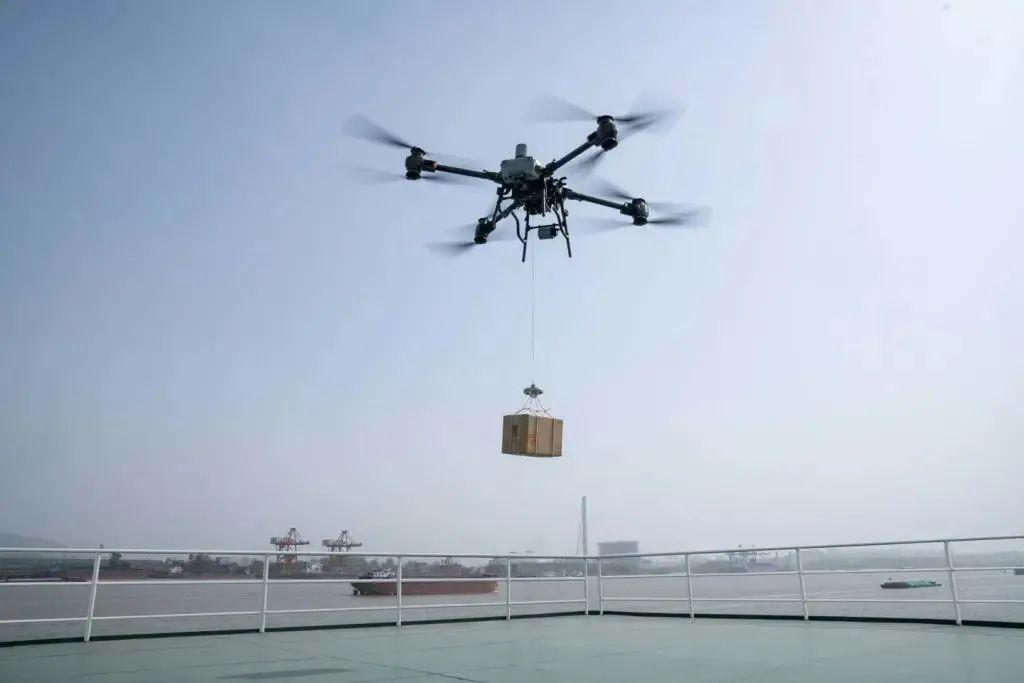
\includegraphics[height = 1.75in]{picture/dji1.jpg}
            \caption{单无人机绳系吊运系统\label{dji1}}
        \end{subfigure}\hfill
        \begin{subfigure}[t]{0.47\textwidth}
            \centering
            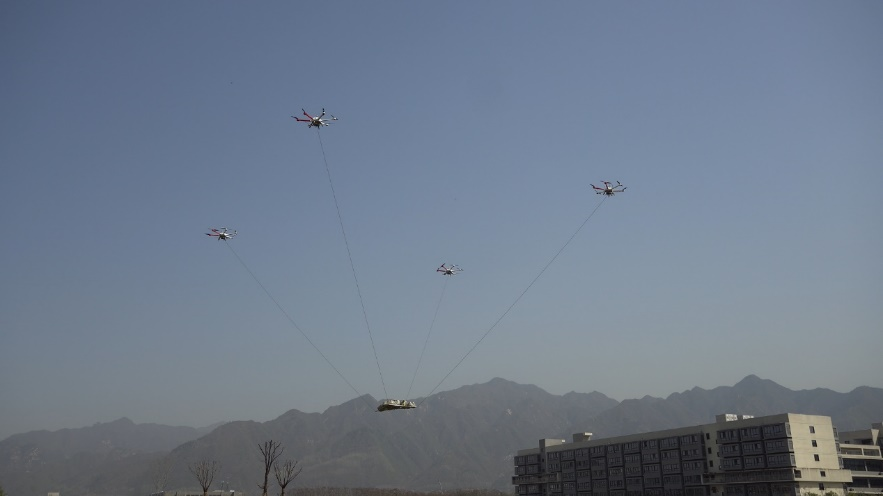
\includegraphics[height = 1.75in]{picture/dji2.png}
            \caption{多无人机绳系吊运系统\label{dji2}}
        \end{subfigure}
    \end{minipage}
    \caption{空中吊挂运输实例}
\end{figure*}
虽然单无人机绳系吊运载荷有以上众多优点,但仍然存在着许多问题:在空中运输过程中,系绳与载荷会形成类似单摆的结构,在载荷晃动的情况下,系绳的拉力会出现不确定性,且难以通过传感器精确观测,这不仅给无人机增添了更多的自由度,甚至可能引发无人机的不稳定性;单无人机在利用吊装方式运输的时候载荷会存在摆动,且当需要运输的载荷重量与无人机的载荷重量相当时,任务可能会受到影响。

为了解决这些问题,采用多个协作式的无人机绳系吊运载荷是一个很有前途的替代方案,即将多架无人机按照期望的队形来分布,并使其在执行任务的过程中保持编队队形平稳飞行,从而圆满完成运输任务。
多无人机绳系吊运系统通过根据有效载荷重量适当调整四旋翼无人机的数量,使这种吊挂式有效载荷配置能够实现最大的有效载荷输送效率,此外这种配置还可以有效控制载荷的姿态,解决了单无人机运输载荷出现摆动的问题,甚至在单无人机发生故障时仍可以完成任务需求。因此多无人机吊运载荷具有可行性高、效率高以及扩展性强等单架无人机无法比拟的优势。本文主要研究\autoref{dji1}中所示的单无人机绳系吊运系统和\autoref{dji2}中所示的多无人机绳系吊运系统。
% 本文主要研究\autoref{dji1}中所示的单无人机绳系吊运系统和\autoref{dji2}中所示的多无人机绳系吊运系统。绳系吊运载荷最初是为紧急响应、救援任务、民用和军事行动中的人力操作直升机而研究的\cite{2020A}。

% 在运输过程中,载荷会对无人机产生了一系列影响,载荷的摆动运动

% 。无人机绳系吊运系统是欠驱动和非线性耦合的,此外无人机的动力学为载荷的摆动运动会引发无人机系统的不稳定性,同时给无人机系统增添了更多的自由度,使得此类系统的控制更具挑战性。

% 在运输过程中,

\section{国内外研究现状}
随着无人机相关理论的快速发展以及试验硬件条件的不断提升,旋翼无人机飞行技术取得了显著进展,特别是全自主飞行的旋翼无人机系统逐渐进入实际应用。国内外多个研究团队积极投入到无人机的基础理论研究,并开展了相关的试验验证工作。本小节将介绍国内外关于无人机绳系吊运系统建模方法、控制方法以及数据驱动控制方法的研究现状。
\subsection{无人机绳系吊运系统建模方法研究现状}
通过建立数学模型来描述被控对象是设计和综合控制器的基础。一个简洁而全面的数学模型能够准确描述被控对象的物理特性,为控制器设计提供有力指导。
在无人机绳系吊运系统的建模过程中,主要考虑的是系绳对四旋翼的约束作用。通过简化对系绳的建模,可以得到绳系无人机的整体模型,下面将介绍几种主要的建模方法。
\subsubsection{单无人机绳系吊运系统建模方法}
关于无人机运输载荷的早期研究始于20世纪90年代末\cite{oshman1999mini,borky1997payload}。在无人机绳系吊运载荷的过程中,系绳的处理是建模系统及四旋翼无人机在起吊、运输和投递阶段所受力的关键因素\cite{qian2020guidance}。在运输阶段,载荷通过系绳传递拉力,而在起吊阶段初期,系绳不传递任何力\cite{guo2020controlling}。为简化建模,通常将这种力的传递简化为系绳是否拉紧\cite{tang2018aggressive}。

\begin{figure}[hbt!]
	\centering
	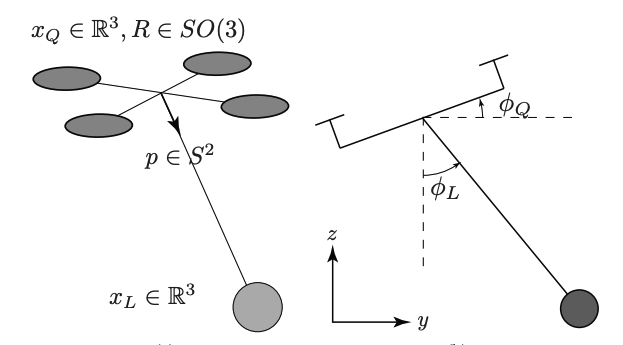
\includegraphics[width=28pc]{picture/1_1.png} 
	\caption{文献\oldcite{sreenath2013trajectory}中带有系绳吊挂载荷的三维四旋翼无人机和平面四旋翼无人机} \label{1_1}
\end{figure}
单无人机的绳系吊运系统动力学模型将载荷表示为质点,将系绳视为无质量刚性杆,该杆在载荷与四旋翼无人机之间保持恒定距离,并且只能通过轴向力进行传递。在这种条件下,在三维场景中,该载荷系统由空间中的两个角度定义,而在平面场景中,一个角度就足够了,类似于摆\cite{sun2021novel},如图\ref{1_1} 所示。

将系绳视为无质量刚性杆的建模方法因其能够更轻松地稳定无人机的位置而被科学界广泛接受。
Lupashin等人\cite{lupashin2013stabilization}提出了一个系绳四旋翼无人机,并将系绳建模为无质量刚性杆,他们利用该系绳作为与用户交互的媒介,从而稳定小型低成本悬停无人机的方向和位置  。通过拉紧系绳,仅使用简单的惯性测量传感器就足以使四旋翼无人机在受到外部干扰后恢复其位置和姿态。沿用该方法,Sreenath 等人\cite{sreenath2013trajectory}对吊挂载荷的系绳进行了建模,将其分为拉紧和零拉力两种情况。在三维场景下,具有非零系绳拉力的系统动态方程具有8个自由度,其中4个是欠驱动的。相反,当系绳不传递拉力时,他们认为无人机和系绳形成独立系统,载荷处于自由下落状态。在两种情况下,他们均通过模拟和实际试验验证了模型。

\begin{figure}[hbt!]
	\centering 
	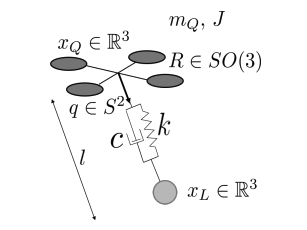
\includegraphics[width=20pc]{picture/1_3.png} 
	\caption{文献\oldcite{kotaru2017dynamics}中带阻尼和线性弹簧的系绳模型} \label{1_3}
\end{figure}
在上述研究中,系绳通常被建模为无质量刚性杆,然而,当四旋翼无人机执行某些任务时,无质量刚性杆模型的局限性显现出来\cite{castillo2019disturbance,estevez2021hybrid}。Klausen 等人\cite{klausen2017nonlinear}在针对激进机动的试验中测试了无质量刚性杆系绳模型,并指出在突然加速期间载荷发生显著偏移,即使无人机达到悬停状态,载荷仍保持低幅度摆动。这些局限性促 使研究人员提出其他系绳模型。Kotaru 等人\cite{kotaru2017dynamics}认为系绳具有弹性,并通过专注于机器人应用研究验证了他们的模型。在这种情况下,系绳的弹性无法忽略,因此刚性杆模型不再适用。为此,他们在系绳模型中加入了阻尼和弹簧(见图 \ref{1_3}),并在不同阻尼和刚度值下测试了系统稳定性,尽管研究仅通过模拟进行验证。Goodarzi 等人\cite{goodarzi2015geometric}提出了另一种新的柔性系绳模型,该模型由一系列不同尺寸的链条组成,并通过球形关节连接(见图 \ref{1_4}),关节之间的连接可以进行延伸,旨在为执行激进机动的无人机载荷系统获得更精确的动力学模型。该方法将载荷建模为由$n$个连接链组成的串联链条,旨在证明系绳无人机在三维飞行机动中稳定性的耦合系统。
% 然而,据现有文献所知,该方案尚未在文献中得到广泛应用。
该模型将系绳建模为由$n$个连接链组成的串联链,并通过球形关节连接如图 \ref{1_4} 所示。这些关节之间的连接可以延伸,旨在为执行激进机动的无人机绳系系统提供更精确的动力学模型。

\begin{figure}[hbt!]
	\centering
	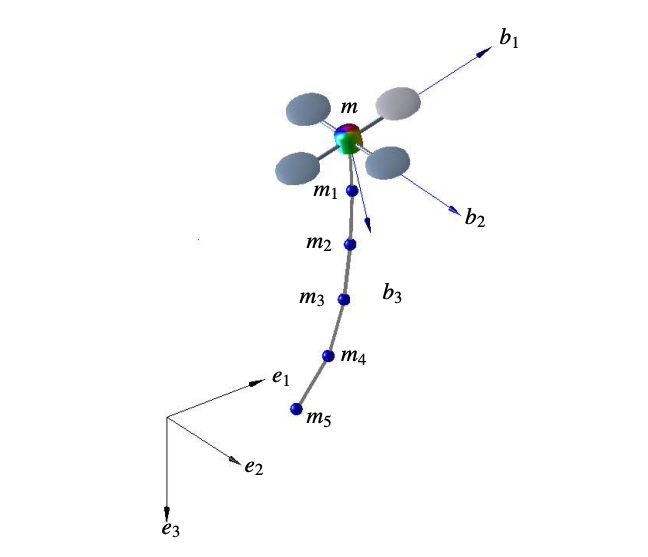
\includegraphics[width=28pc]{picture/1_4.png} 
	\caption{文献\oldcite{goodarzi2015geometric}中的柔性系绳模型示意图} \label{1_4}
\end{figure}
\subsubsection{多无人机绳系吊运系统建模方法}
为了适应多种载荷类型,研究人家提出了系绳连接的多无人机协同运输方式。早在2011年,Vijay Kumar团队\cite{Gouttefarde2006,Gouttefarde2011}基于多无人机绳系吊运系统与绳驱并联操作机器人\cite{Gouttefarde2006,Gouttefarde2011}的相似性,将绳驱并联操作机器人的控制方法拓展应用于多无人机绳系吊运系统上,将系绳视为无质量的刚性杆,对系统进行了精确建模\cite{Fink2011,michael2011cooperative,Jiang2013}。
% 此外,该团队提出了一种通过牵引系绳运输圆盘型载荷的模型\cite{goodarzi2015geometric},该问题类似于三维空间中的系绳驱动并联操控器,因两者均通过改变机器人位置来控制载荷姿态;
四旋翼机通过系绳牵引改变载荷的定向如图 \ref{1_5} 所示。
Lee 等人采用拉格朗日方程对系统进行建模,研究了质点载荷\cite{lee2013geometric}和刚体载荷\cite{lee2017geometric}。
在此基础上,牛顿-欧拉法被应用于多无人机绳系系统的建模,并引入零交互力条件\cite{cardona2019cooperative}。Shirani等人\cite{shirani2019cooperative}则采用20世纪90年代提出的Udwadia–Kalaba方程\cite{udwadia1992new,udwadia1996equations},简化了多无人机绳系吊运系统的动力学模型。

\begin{figure}[hbt!]
	\centering
	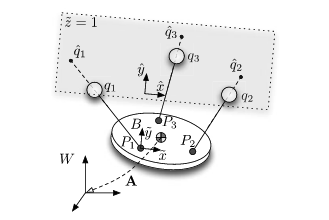
\includegraphics[width=28pc]{picture/1_5.png} 
	\caption{文献\oldcite{michael2011cooperative}中的多无人机绳系吊运系统} \label{1_5}
\end{figure}
Pizetta 等人\cite{pizetta2019avoiding}提出了另一种系绳建模方案,采用弹性系绳模型,并依靠系绳的牵引力来抵消载荷对无人机产生的扰动。此外,该团队证明了该方案在载荷从地面起吊的情况下是有效的。对于刚性二维载荷的吊运,Goodarzi等人\cite{goodarzi2016stabilization}通过将系绳系统建模为一系列由球形关节连接的链条来实现。正如文献\oldcite{Goodarzi2015}所述,该方案在无人机载荷运输中具有较强的鲁棒性。对于在吊运过程中的系绳的拉紧和零拉力两种情况,Lopez-Guede等人\cite{estevez2022hybrid}提出了一种混合抛物线和链条切换模型,以防止在激进机动或急转弯时,无人机编队因过于接近而导致链条结构坍塌。
这一基于悬链线的系绳建模方法也被其他研究团队\cite{d2021catenary,abhishek2021towards}采用,并通过试验验证了其有效性,但这些研究均仅采用两架旋翼无人机进行编队。

\begin{figure}[hbt!]
	\centering
	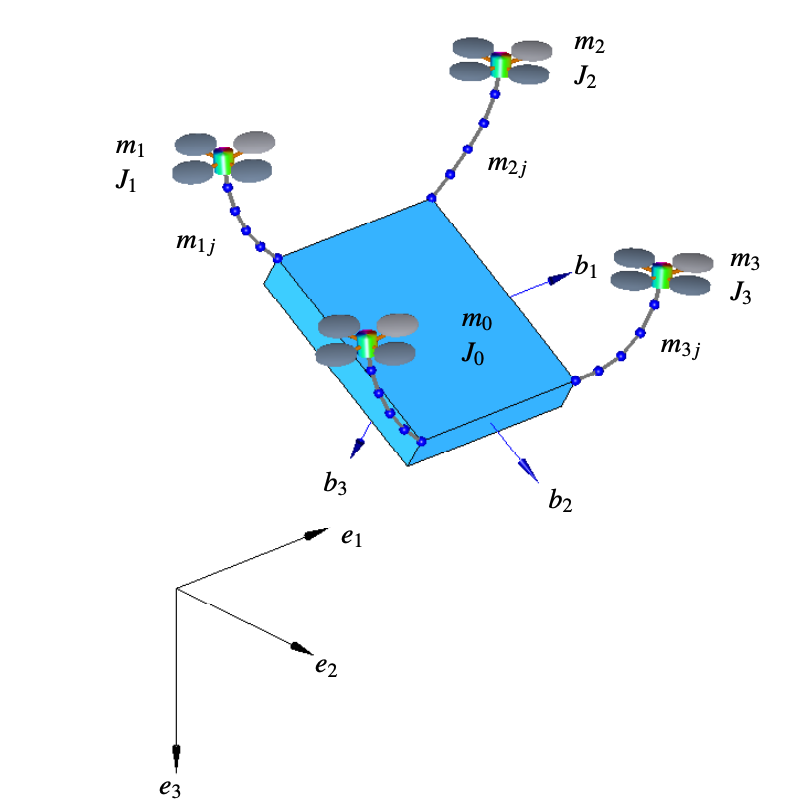
\includegraphics[width=24pc]{picture/1_6.png} 
	\caption{文献\oldcite{goodarzi2016stabilization}中的多无人机绳系吊运系统} \label{1_6}
\end{figure}
% 此外,多机器人运输方案中,很少有研究考虑起飞或着陆过程。尽管 Goodarzi 等人\cite{goodarzi2015dynamics} 以及Kumar等人\cite{michael2011cooperative}的试验表明其系统能够实现起降,但相关文献并未描述系绳在过渡阶段的数学建模。在这些阶段纳入系绳的动态特性会增加计算成本。
在多无人机系绳吊挂载荷的建模方法中,通常采用简化策略以降低计算复杂度。例如,Bacelar 等人\cite{bacelar2020board}提出了使用两架 AR Drone 2.0 四旋翼无人机运输吊挂载荷的方法,假设系绳始终处于拉紧状态。随后,Pizetta 等人提出了由两架四旋翼无人机通过两根由弹簧和阻尼器连接的点质量组成的系绳来运输点质量载荷的系统。该系绳模型能够吸收与地面的接触冲击,并线性减少系绳的拉力。Geng 等人\cite{geng2020cooperative}和 Goodman 等人\cite{goodman2023geometric} 也采用了相同的系绳动力学模型。尽管弹性系绳有助于缓解作用在杆上的冲击力,但过度的振荡可能引发不必要的强制运动,危及协作任务的安全性。因此,在运输过程中,采用具有更高刚度和阻尼的弹性系绳对于保护载荷至关重要。例如,Goodman 等人\cite{goodman2022geometric}在后续研究中通过仿真验证了他们的结果,而 Gabellieri 等人\cite{gabellieri2023equilibria}则通过实际试验验证了他们的方案。

\begin{figure}[hbt!]
	\centering
	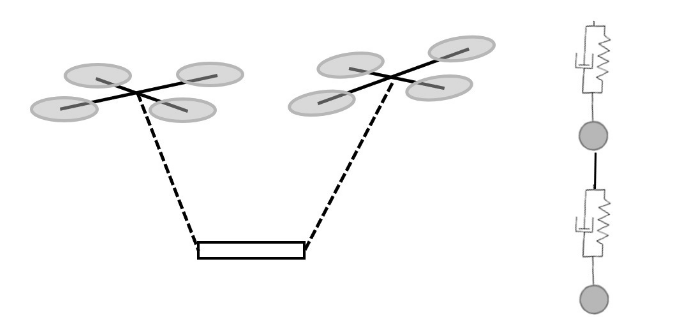
\includegraphics[width=28pc]{picture/1_8.png} 
	\caption{文献\oldcite{doakhan2023cooperative, doakhan2023robust}中的多无人机绳系吊运系统} \label{1_8}
\end{figure}
% 近年来,研究趋势倾向于扩展系绳模型,使其在达到特定高度阈值时,从松弛状态切换至拉紧状态\cite{rao2023integrated,arab2022cooperative,doakhan2023robust,mohammadi2021passivity}。这种方法在数学上相对简单,已成为试验中常用的吊挂载荷方案,适用于包含载荷提升的平稳机动任务。然而,这些研究主要局限于平稳的机动操作。

\subsection{无人机绳系吊运系统控制方法研究现状}
由于载荷的吊运通常会引入动态扰动,特别是由于绳系和载荷本身的摆动效应,导致无人机的飞行性能受到显著影响。为了实现对无人机绳系吊运系统的高效稳定控制,确保其能够完成各类任务,众多控制算法已经得到了应用,并取得了良好的效果。接下来,将对其中一些常用的控制算法进行介绍。
\subsubsection{单无人机绳系吊运系统控制方法}
在飞行过程中,载荷会引入被动动态效应,这些效应可能来自系绳或载荷本身,并导致摆动,从而改变无人机的动力学特性并影响其动态性能。针对载荷引起的扰动,最常见的应对方式是通过最小化载荷摆动来稳定系统\cite{lv2022finite,2019An}。此外,Foehn等人\cite{Foehn-RSS-17}采用反馈控制方法以跟踪期望的载荷轨迹,通过轨迹规划算法解决带载四旋翼无人机的多体系统动力学问题。

Sreenath和Cruz等人\cite{sreenath2013trajectory,cruz2015lift}提出了一种混合动力学模型,将系绳模型划分为不同的子系统。在这些混合动力学模型中,每个子系统配备专门的控制器,并由监督系统在简单控制器之间进行切换。相比之下,Guo 和Villa等人\cite{guo2020multiple,villa2021cooperative}则专注于探索通用解决方案,以解决悬缆运输问题,无论任务处于哪个阶段。

在载荷运输任务中,精准的轨迹跟踪至关重要。Lee 等人\cite{lee2015collision,lee2017geometric}提出的几何控制器能够使载荷的位置和姿态精确跟踪期望路径。该方法采用 Voronoi 镶嵌技术进行轨迹规划,并考虑了避障相关的约束条件。Sreenath 等人\cite{sreenath2013trajectory}研究了载荷在大幅摆动并经历零拉力瞬间时的控制问题,设计了一种反馈控制器,并证明该系统具有微分平坦特性,可有效应用于无人机与载荷系统的控制。

针对外部扰动,Qian 和 Liu\cite{qian2019path}研究了无人机在有风条件下进行载荷运输的情况。他们实现了一种级联闭环控制配置,其中外环基于不确定性与扰动估计器 (UDE) 提出了平移控制律,以稳定无人机沿预定轨迹飞行,并通过低通滤波器估计总扰动。内环采用姿态跟踪控制器,通过调整升力矢量方向使其与推力矢量方向保持一致,从而渐近跟踪外环生成的参考力。
Cabecinhas 等人\cite{cabecinhas2019trajectory}开发了一种考虑不确定扰动参数和载荷的四旋翼吊挂载荷模型,旨在设计动态反馈控制器,使载荷沿嵌入轨迹平稳移动,并引导系统沿指定路径运行。同样,Tagliabue 等人\cite{2019Robust}基于鲁棒控制理论,在系统存在多种物理不确定性的情况下,确保其在最恶劣场景下的稳定性。

随着任务复杂性的增加,尤其是在紧急搜救等高机动性任务中,无人机需要在面对模型不确定性(如未知阻力系数)和外部扰动(如载荷变化或突风)时,精准跟踪飞行轨迹以完成复杂任务。
Tal等人\cite{2021Accurate}的研究展示了通过增量非线性动态逆 (INDI) 结合级联几何控制器,实现四旋翼无人机对高动态轨迹的精确跟踪。Sreenath 等人\cite{sreenath2013geometric}构建了一种几何控制器,在载荷发生大幅摆动的情况下,实现了短时内的精准位置跟踪,适用于激进机动。然而,正如文献\oldcite{torrente2021data,sun2022comparative}指出的,INDI 和传统几何控制器完全属于反应式控制,缺乏在预测时域内的规划能力。

近年来,研究人员逐渐青睐模型预测控制器 (MPC) 以实现载荷运输的最优轨迹跟踪\cite{urbina2021predictive}。MPC 适用于分布式和多层次控制系统的设计,其核心在于将无人机的参考轨迹计算作为约束优化问题的解。例如,Lee 等人\cite{lee2015study}将 MPC 与比例微分 (PD) 控制器相结合,利用载荷摆动角误差作为输入,修正沿规划轨迹的平移控制器。Estevez 等人\cite{estevez2021hybrid}证明该控制策略同样适用于双摆载荷模型。Son等人\cite{son2018model}在存在突发障碍的场景下使用顺序线性二次 (SLQ) 控制的 MPC,试验结果表明该空中系统能够在动态场景中平稳飞行。

尽管非线性模型预测控制 (NMPC) 方法具有优越性能,但计算成本较高\cite{norouzi2022deep}。因此,部分研究人员考虑采用线性模型预测控制 (LMPC) 作为替代方案。然而,现有许多 LMPC 研究仅关注位置控制\cite{bangura2014real}或基于小角度假设的运动控制\cite{alexis2014trajectory}。由于 LMPC 无法充分捕捉旋转动力学中的非线性,其性能通常不如 NMPC 方法\cite{nguyen2021model}。

\subsubsection{多无人机绳系吊运系统控制方法}
为解决使用四旋翼无人机和系绳进行协同吊装运输载荷的难题,Maza 等人\cite{maza2010multi}设计了一种PID控制器。然而,该控制器方法无法有效减小欠阻尼系统中的振荡。Bacelar 等人\cite{bacelar2020board}开发了一种基于两架无人机的协同载荷运输控制方法,结合了线性二次调节器 (LQR) 控制器与卡尔曼滤波器。该方法通过两架配备超声波高度计、惯性测量单元 (IMU) 和前置摄像头的商用四旋翼无人机进行了试验验证。

Ariyibi 等人\cite{ariyibi2020quaternion}提出了一种用于两架四旋翼无人机运输吊挂载荷的分层控制系统。该系统在位置环中采用线性控制器,在姿态环中使用基于四元数的非线性控制器。研究人员通过仿真代码验证了该控制器对刚性和柔性载荷的适用性。Klausen 等人\cite{klausen2018cooperative}开发了一种针对未知质量、能够抵御环境干扰的协同算法。该控制算法是分布式的,每架四旋翼无人机利用其邻居的相对速度和位置来实现期望的编队形状。

Tognon等人\cite{tognon2018aerial}提出了一种基于李雅普诺夫的分布式控制器,用于两架无人机对系绳吊挂载荷的空中操控。该工作的目标是在不依赖主从阻抗控制器进行通信的情况下,调节载荷的位置和姿态。Wehbeh等人\cite{wehbeh2020distributed}展示了一种基于模型预测控制 (MPC) 的分布式协同运输方法。

Gimenez 等人\cite{gimenez2018multi}提出了一种新的运动学编队控制器,利用零空间理论使两架旋翼无人机通过柔性系绳吊挂载荷并跟随期望轨迹。该控制器考虑了风扰动和避障问题。在后续研究中,该团队使用相同控制技术,通过试验验证了两架旋翼无人机运输刚性载荷的着陆阶段\cite{gimenez2020control}。

最后,Lee 等人\cite{lee2013geometric}将几何控制器扩展至多架四旋翼无人机团队载荷运输。然而,这些方法均假设载荷为质点,而实际载荷通常具有不可忽略的几何尺寸,有时甚至与无人机尺寸相当。为克服这一限制,该团队在此基础上设计了一种几何非线性控制器,用于刚体载荷的群体运输\cite{lee2017geometric}。然而,该方法需要已知系绳的方向和角速度,而这些参数在实际场景中难以计算。因此,Sharma 等人\cite{sharma2023geometric}提出了一种动态系统模型,该模型考虑了载荷与旋翼无人机之间的耦合关系,从而创建了一种以四旋翼为中心的方法,避免了上述难以获取的参数。

% 然而,以上提到的研究大多忽略了载荷与无人机之间的耦合效应。
% 超过两个四旋翼的多升系统引入了系绳拉力的冗余性[15],导致拉力在四旋翼之间的分布不唯一。在[16]–[18]中,作者提出了系绳拉力分布的最小范数解法。相比之下,Geng等人[19][20]利用这种冗余性,在四旋翼的多升系统中实现了最佳拉力分布,同时保证了安全的旋翼间隔,并考虑了四旋翼的推力限制。此外,最近的研究工作[21][22]将这种冗余性纳入了集中式MPC框架,不仅确保了安全约束,还通过充分考虑系统的非线性动力学,改善了系统的机动性。

% 如上述工作[13][19]–[23]所示,优化方法对于多升系统是有效的,因为它们能够管理约束条件和非线性动力学。然而,这些方法的性能在很大程度上取决于超参数的调节,包括代价函数中的加权和参考值。这些超参数的调节通常需要大量的人工努力,并且受到系绳之间复杂的动态相互连接的影响。为了简化这一过程,通常需要做出保守的假设,如将载荷视为点质量,假设为准静态飞行,并且拉力分布均匀,这可能导致次优结果。随着四旋翼数量的增加以及当其最佳值是动态变化且相互关联时(例如,载荷的质量分布不均且系统必须动态调整配置以避开障碍物),手动选择这些参数的挑战会更大。



\subsection{数据驱动方法研究现状}
近年来,计算机硬件和软件技术飞速发展,“大数据”作为一种概念由计算领域发端,之后逐渐延伸到各个领域。在控制领域中,随着系统的复杂性逐渐增加,数据的获取变得更加容易,基于数据驱动的建模和控制方法在的应用也逐渐成为研究热点。数据驱动方法的提出源于Ziegler和Nichols的经典工作\cite{ziegler1942optimum},该方法为后续的自适应控制\cite{wittenmark1989adaptive}和神经网络理论\cite{werbos1989neural}的研究奠定了基础。

使用无人机进行快速灵活的机动操作,需要针对被控对象建立精确动力学模型。然而,对于刚柔混合的无人机绳系吊装系统,由于摩擦、空气动力学、系绳上的力突变等因素的影响,传统的动力学模型往往无法充分捕捉到系统的复杂行为。
许多研究者开始绕过经典的基于模型的技术,转而采用数据驱动的方法\cite{hou2013model},而无模型和基于模型的数据驱动建模方法被认为是无人机进行运输和操纵的最优控制策略。

无模型数据驱动建模方法的核心思想是通过观测和分析系统的输入输出数据,直接从数据中提取系统的动力学规律,而无需明确的物理模型。Sacks和Chen等人\cite{sacks2023learning,chen2022gaussian}通过高斯过程来以概率逼近系统的动力学微分方程,Lusch和 He 等人\cite{lusch2018deep,hewing2019cautious}通过使用深度强化学习的数据驱动技术,成功地识别了复杂系统的底层模型,Finn等人\cite{finn2017model}提出了一种通用的元学习框架,通过优化模型的初始化参数,使得模型能够在面对新任务时快速适应并取得较好性能,Belkhale等人\cite{belkhale2021model}提出一种基于元学习的无模型数据驱动方法,在连接飞行数据的几秒钟内"学习如何学习"变化的动力学模型,能够快速适应动态变化的环境。无模型的数据驱动建模的优势在于无需任何被控对象的先验知识,仅需被控对象的输入输出数据,但是针对这类方法建立的模型无法分析系统 的内在动力学特性,对于实际应用中的无人机来说,由于需要大量的数据进行训仍然存在实时自适应控制能力的不足。


与无模型方法相比,基于模型的数据驱动方法通常在已知部分系统动力学模型的基础上,进一步学习系统中被控对象中存在部分动力学难以建立或者无法建立的的动力学。
Shi等人\cite{o2022neural}提出了通过对无人机在风扰中的情形进行快速自适应学习的框架,该方法结合了系统的已知动力学与从数据中学习到的外部扰动模型,从而提高了系统在复杂环境下的鲁棒性。Salzmann等人\cite{salzmann2023real}和Torrente等人\cite{torrente2021data}使用深度学习估计四旋翼动力学模型未建模部分的动力学,然后设计模型预测控制器控制四旋翼通过障碍物,Bauersfeld等人\cite{Bauersfeld2021}提出了一种结合了基于BEM理论的最先进旋翼模型与深度神经网络表示的残差力和力矩项的方法,能够准确捕捉复杂的空气动力效应。这种基于模型的数据驱动方法不仅能够充分利用已知物理模型的精确性,还能通过神经网络的学习能力弥补模型的不足,提高系统的适应性。

为了克服神经网络在数据匮乏时可能带来的性能下降,许多研究尝试将基于模型的数据驱动方法与传统的控制算法相结合,从而更好地利用两者的优点。模型预测控制(MPC)作为一种强大的基于模型的方法,能够同时处理复杂的非线性动态系统,并满足不同的状态和输入约束\cite{neunert2016fast},因此,成为了与数据驱动方法结合的理想选择。文献\oldcite{torrente2021data}提出了一种方法,通过使用高斯过程来对气动效应进行建模,并将其融入MPC中,实现了高效和精确的实时反馈控制。文献\oldcite{song2022policy}则将MPC建模为一个参数化控制器,其中难以优化的决策变量表示为高层策略,通过策略优化来提高控制效果。文献\oldcite{salzmann2023real}提出了一个实时神经网络模型预测控制框架,该框架通过有效集成大型复杂神经网络结构,使得系统能够在动态环境中实时进行反馈控制。

% 近年来,随着深度学习和强化学习技术的迅猛发展,越来越多的学者开始探讨如何利用深度神经网络(DNN)和强化学习(RL)直接对控制器进行学习。Koch等人\ref{koch2019reinforcement} 将强化学习应用于低级姿态控制,研究表明,通过PPO训练的学习型低级控制器在几乎所有指标上均优于完全调优的PID控制器;Lambert等人\ref{lambert2019low} 则采用基于模型的强化学习方法进行未知动态系统的低级控制;Li等人\ref{li2020aggressive} 通过离线训练网络策略模仿模型基控制器生成的控制命令,成功实现了四旋翼的激进在线控制。类似地,文献\oldcite{sanchez2018real} 研究了深度神经网络在自主着陆问题中的实时最优控制。此外,相关研究还表明,强化学习能够有效地找到最优控制器\ref{ferede2024end} 或高度自适应的控制器\ref{sacks2024deep}。

\section{现有研究总结与分析}
(1)建模方法:
目前在进行无人机绳系吊运系统的动力学分析时,大多数研究采用了简化的模型。这种简化方式虽然可以减少计算复杂度,但无法精确描述绳系的真实动力学特性,特别是系绳的变形、时变长度和柔性特性。随着绳系无人机任务的复杂化和高精度要求的提高,现有的建模方式已无法满足实际需求,特别是在大范围运动、大变形的场景下,模型的精度和可靠性受到严重制约。本文拟采用基于数据驱动的建模方法,通过对外部非线性项的预测学习,构建能够准确反映系绳柔性特性和动态变化的模型。

(2)参数调整:
现有无人机绳系吊运系统的控制器设计主要基于简化物理模型,这种设计方法对模型具有较强依赖性,需要进行大量参数调整以保证控制性能的稳定性和精度。然而,真实的环境往往充满不确定性和变化,且无人机和绳系的耦合动力学高度复杂,模型的参数往往难以精准确定,尤其是在多变的操作环境中,控制器的鲁棒性和适应性较差。本文拟采用基于数据驱动的控制方法,通过对控制器中的自适应参数进行调节,提高系统在复杂环境中的适应性和鲁棒性。

(3)数据采集:
数据驱动方法在无人机绳系吊运系统建模与控制中的应用依赖于大量高质量历史观测数据。然而,实际环境的不确定性导致高质量数据的获取较为困难,这直接影响了模型的环境适应性。为应对这一挑战,物理仿真引擎的应用可有效弥补实际观测数据的不足。本文拟采用多物理仿真引擎对比分析的方法,精确模拟系绳与无人机间的耦合动力学特性,在保证计算效率的同时生成高质量仿真数据,为模型的建立与优化提供可靠的数据支撑。

\section{研究内容与章节安排}
%基于涡流效应的空间翻滚目标消旋稳定控制,属于电磁消旋方法的一种。
%本文各章节的主要内容介绍如下。
% 本文旨在研究无人机绳系吊运控制中的关键问题,提出数据驱动的方法以提升系统性能。主要研究内容如下:

第一章为绪论。介绍了无人机绳系吊运系统的相关研究背景和意义,同时对目前的国内外发展和研究现状做了系统的说明和详细的介绍。在广泛查阅现有文献的基础上,针对无人机绳系吊运系统的建模、控制方法以及最新的数据驱动控制方法做了充分论述。

第二章为无人机绳系吊运系统建模。针对单无人机和多无人机的绳系吊运系统,建立了详细的动力学模型。对于单无人机系统,采用欧拉-拉格朗日方法描述无人机与吊挂载荷之间的动态关系。对于多无人机系统,在单无人机系统的基础上考虑了多机协同作用下的复杂动力学特性,建立出一个完整的系统动力学模型,为控制器设计提供了可靠依据。 

第三章为数据驱动建模下的单无人机吊运控制。针对系统中存在的连续变化的干扰力和力矩,基于Koopman算子理论,设计了基于数据驱动的未知外力和力矩捕获方案,通过将非线性系统升维为线性系统,实现对未知复杂动力学的有效预测,并用Lipschitz 约束来限制预测误差。在此基础上,通过将数据驱动方法预测得到的模型与无人机名义模型相结合,并将其集成至模型预测控制框架中,显著提升了系统的鲁棒控制性能。

第四章为基于数据驱动的多无人机吊运控制。针对多无人机控制中的手动调参问题,使用自适应学习的超参数优化方法来对分布式模型预测控制的参数进行调节。首先使用分布式灵敏度传播得到 MPC 中关键参数的实际系统状态灵敏度,在此基础上结合深度神经网络设计了分布式策略梯度学习算法实现控制参数的自适应调整,提高了多无人机系统的协调控制性能。

第五章为物理引擎仿真与飞行试验验证。搭建了基于Drake、Gazebo和MuJoCo等物理引擎的仿真平台,对所提出的控制方法进行了验证。此外,设计了试验系统,进行了实际飞行试验,验证了控制策略的有效性和可行性。

最后一章为总结和展望。对全文的研究内容进行了总结,并对未来的研究方向进行了展望。

通过上述研究,本文为无人机绳系吊运控制提供了新的数据驱动方法,提升了系统的建模精度、控制性能和鲁棒性,为无人机在复杂环境下的吊运任务奠定了理论和实践基础。
论文整体架构如图 \ref{1_0} 所示:

\begin{figure}[hbt!]
	\centering
	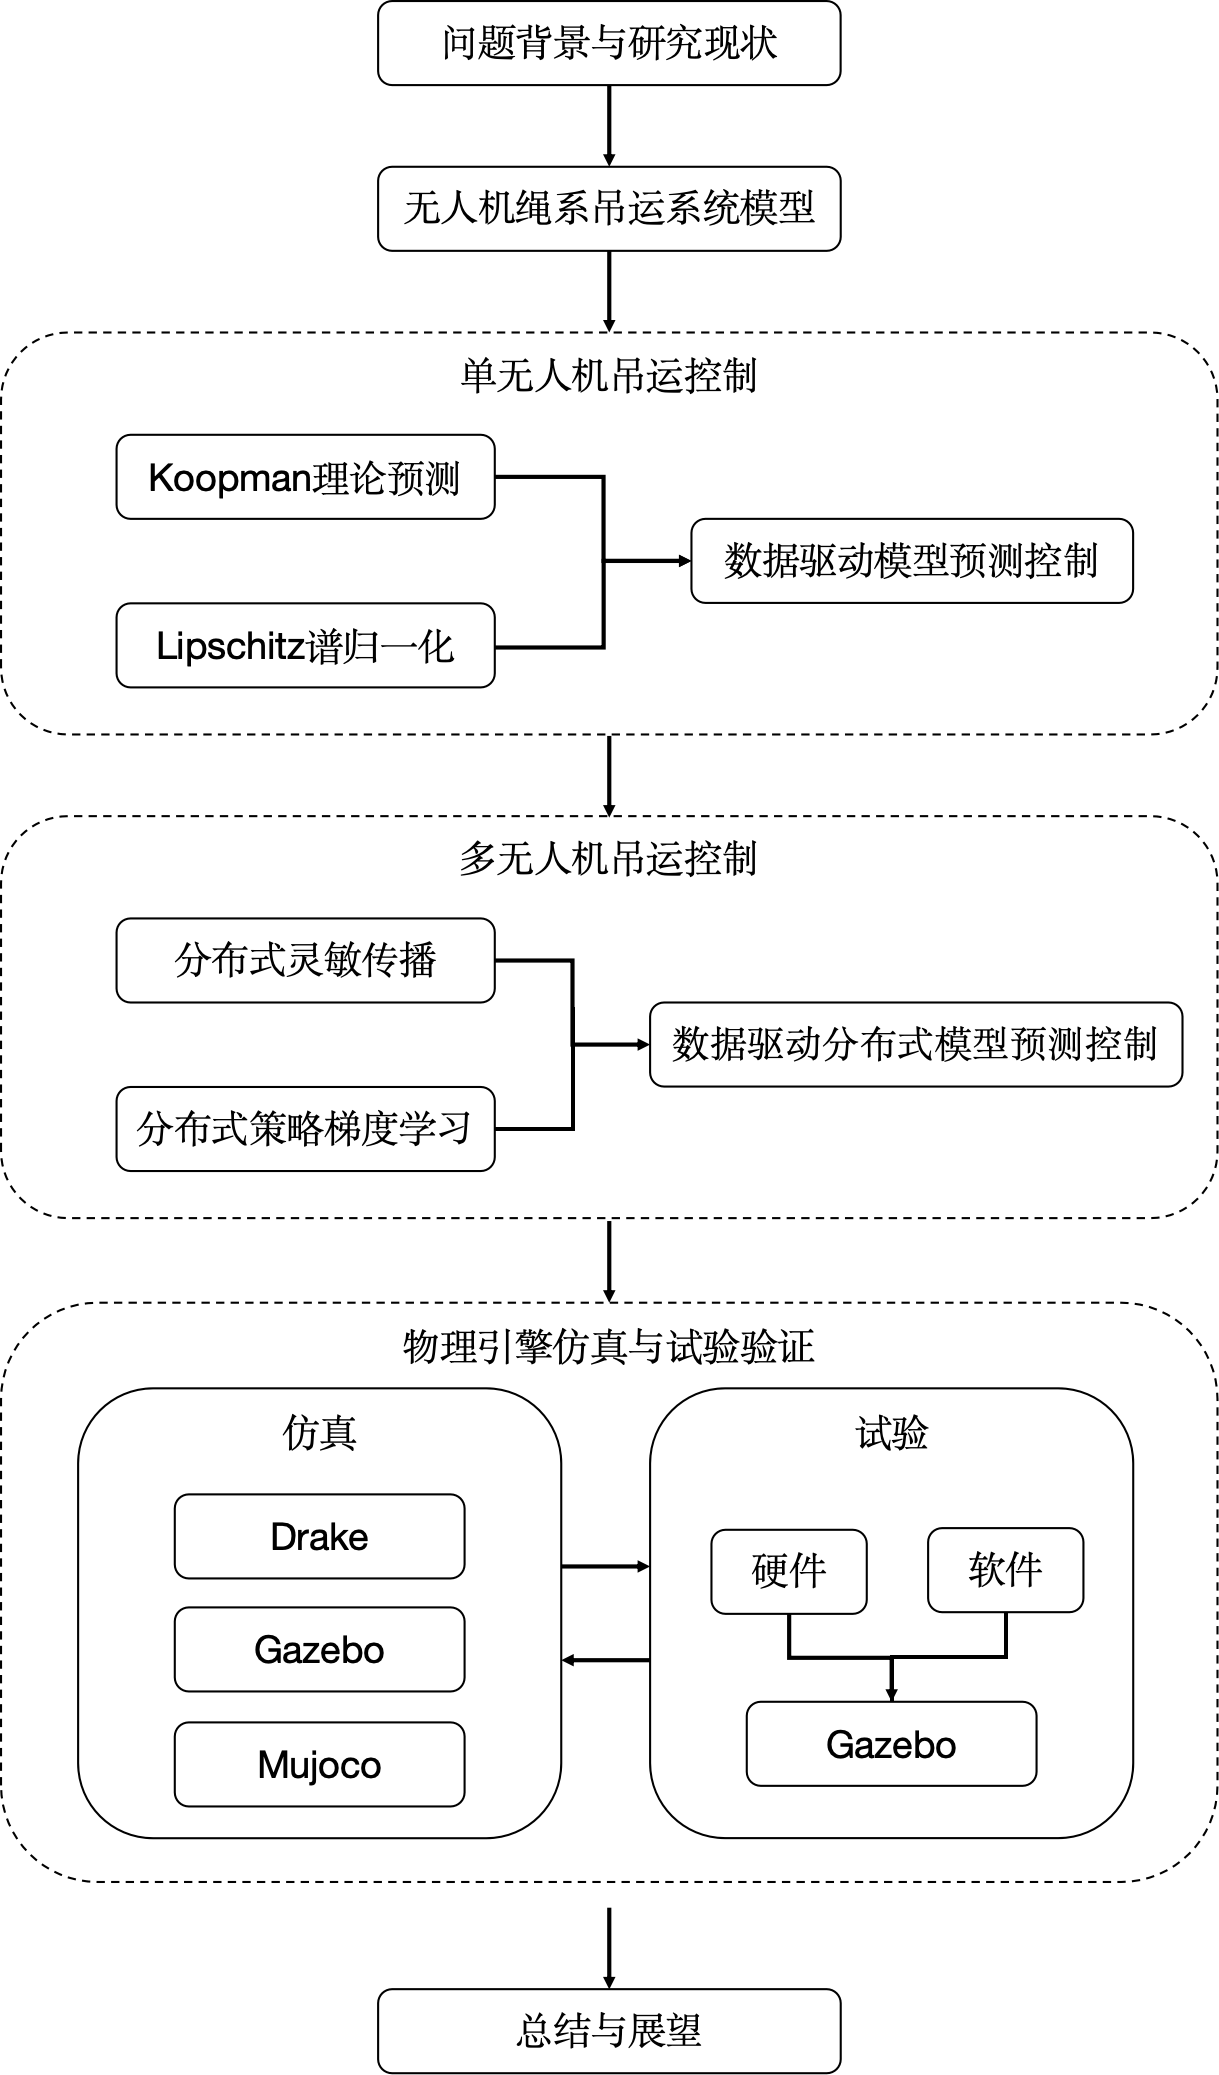
\includegraphics[width=26pc]{picture/1_0.png} 
	\caption{论文研究框架} \label{1_0}
\end{figure}

\cleardoublepage

\chapter{无人机绳系吊运系统建模}
\chaptermark{无人机绳系吊运系统建模}
本文的研究对象是四旋翼无人机绳系吊运系统,其由三个子系统构成:四旋翼无人机、系绳以及吊运的载荷。该系统是一个多输入多输出的欠驱动系统,载荷与无人机受到了系绳的约束,为了能够从基本原理上对该系统有一个完整认识,本章首先推导四旋翼无人机的模型,然后基于拉格朗日建模方法,建立单无人机绳系吊运系统的模型,并进一步推广得到多无人机绳系吊运系统的模型中,以此作为控制模型的基础。

\section{无人机的数学模型}
% 四旋翼无人机绳系吊运系统是一个复杂的飞行控制系统,其中四旋翼无人机由四个旋翼组成,并固定在刚性交叉结构上,载荷通过系绳与四旋翼无人机主体相连。
要深入分析绳系吊运系统的动力学特性,首先需要理解四旋翼无人机自身的动力学原理。四旋翼无人机是一种基于旋翼驱动的飞行器,通过四个旋翼的推力实现飞行和姿态控制。
为了平衡飞行过程中的力矩,四旋翼无人机采用两对相对旋转的转子配置,其中一对沿顺时针方向旋转,另一对沿逆时针方向旋转。该系统具有高度非线性的动力学特性,并且是一个典型的欠驱动系统,拥有六个自由度和四个控制输入(即旋翼转速)。通过调整各旋翼的转速,可以改变四旋翼无人机的整体推力和姿态力矩,进而实现对飞行高度、位置和方向的控制。如图 \ref{2_1} 所示,四旋翼无人机的结构呈现为四个旋翼交叉对称布置,其中相对的两个旋翼沿相同方向旋转,通过调节各旋翼的角速度差异,可以精确控制无人机的升降、偏航以及横滚和俯仰运动。

\begin{figure}[hbt!]
	\centering
	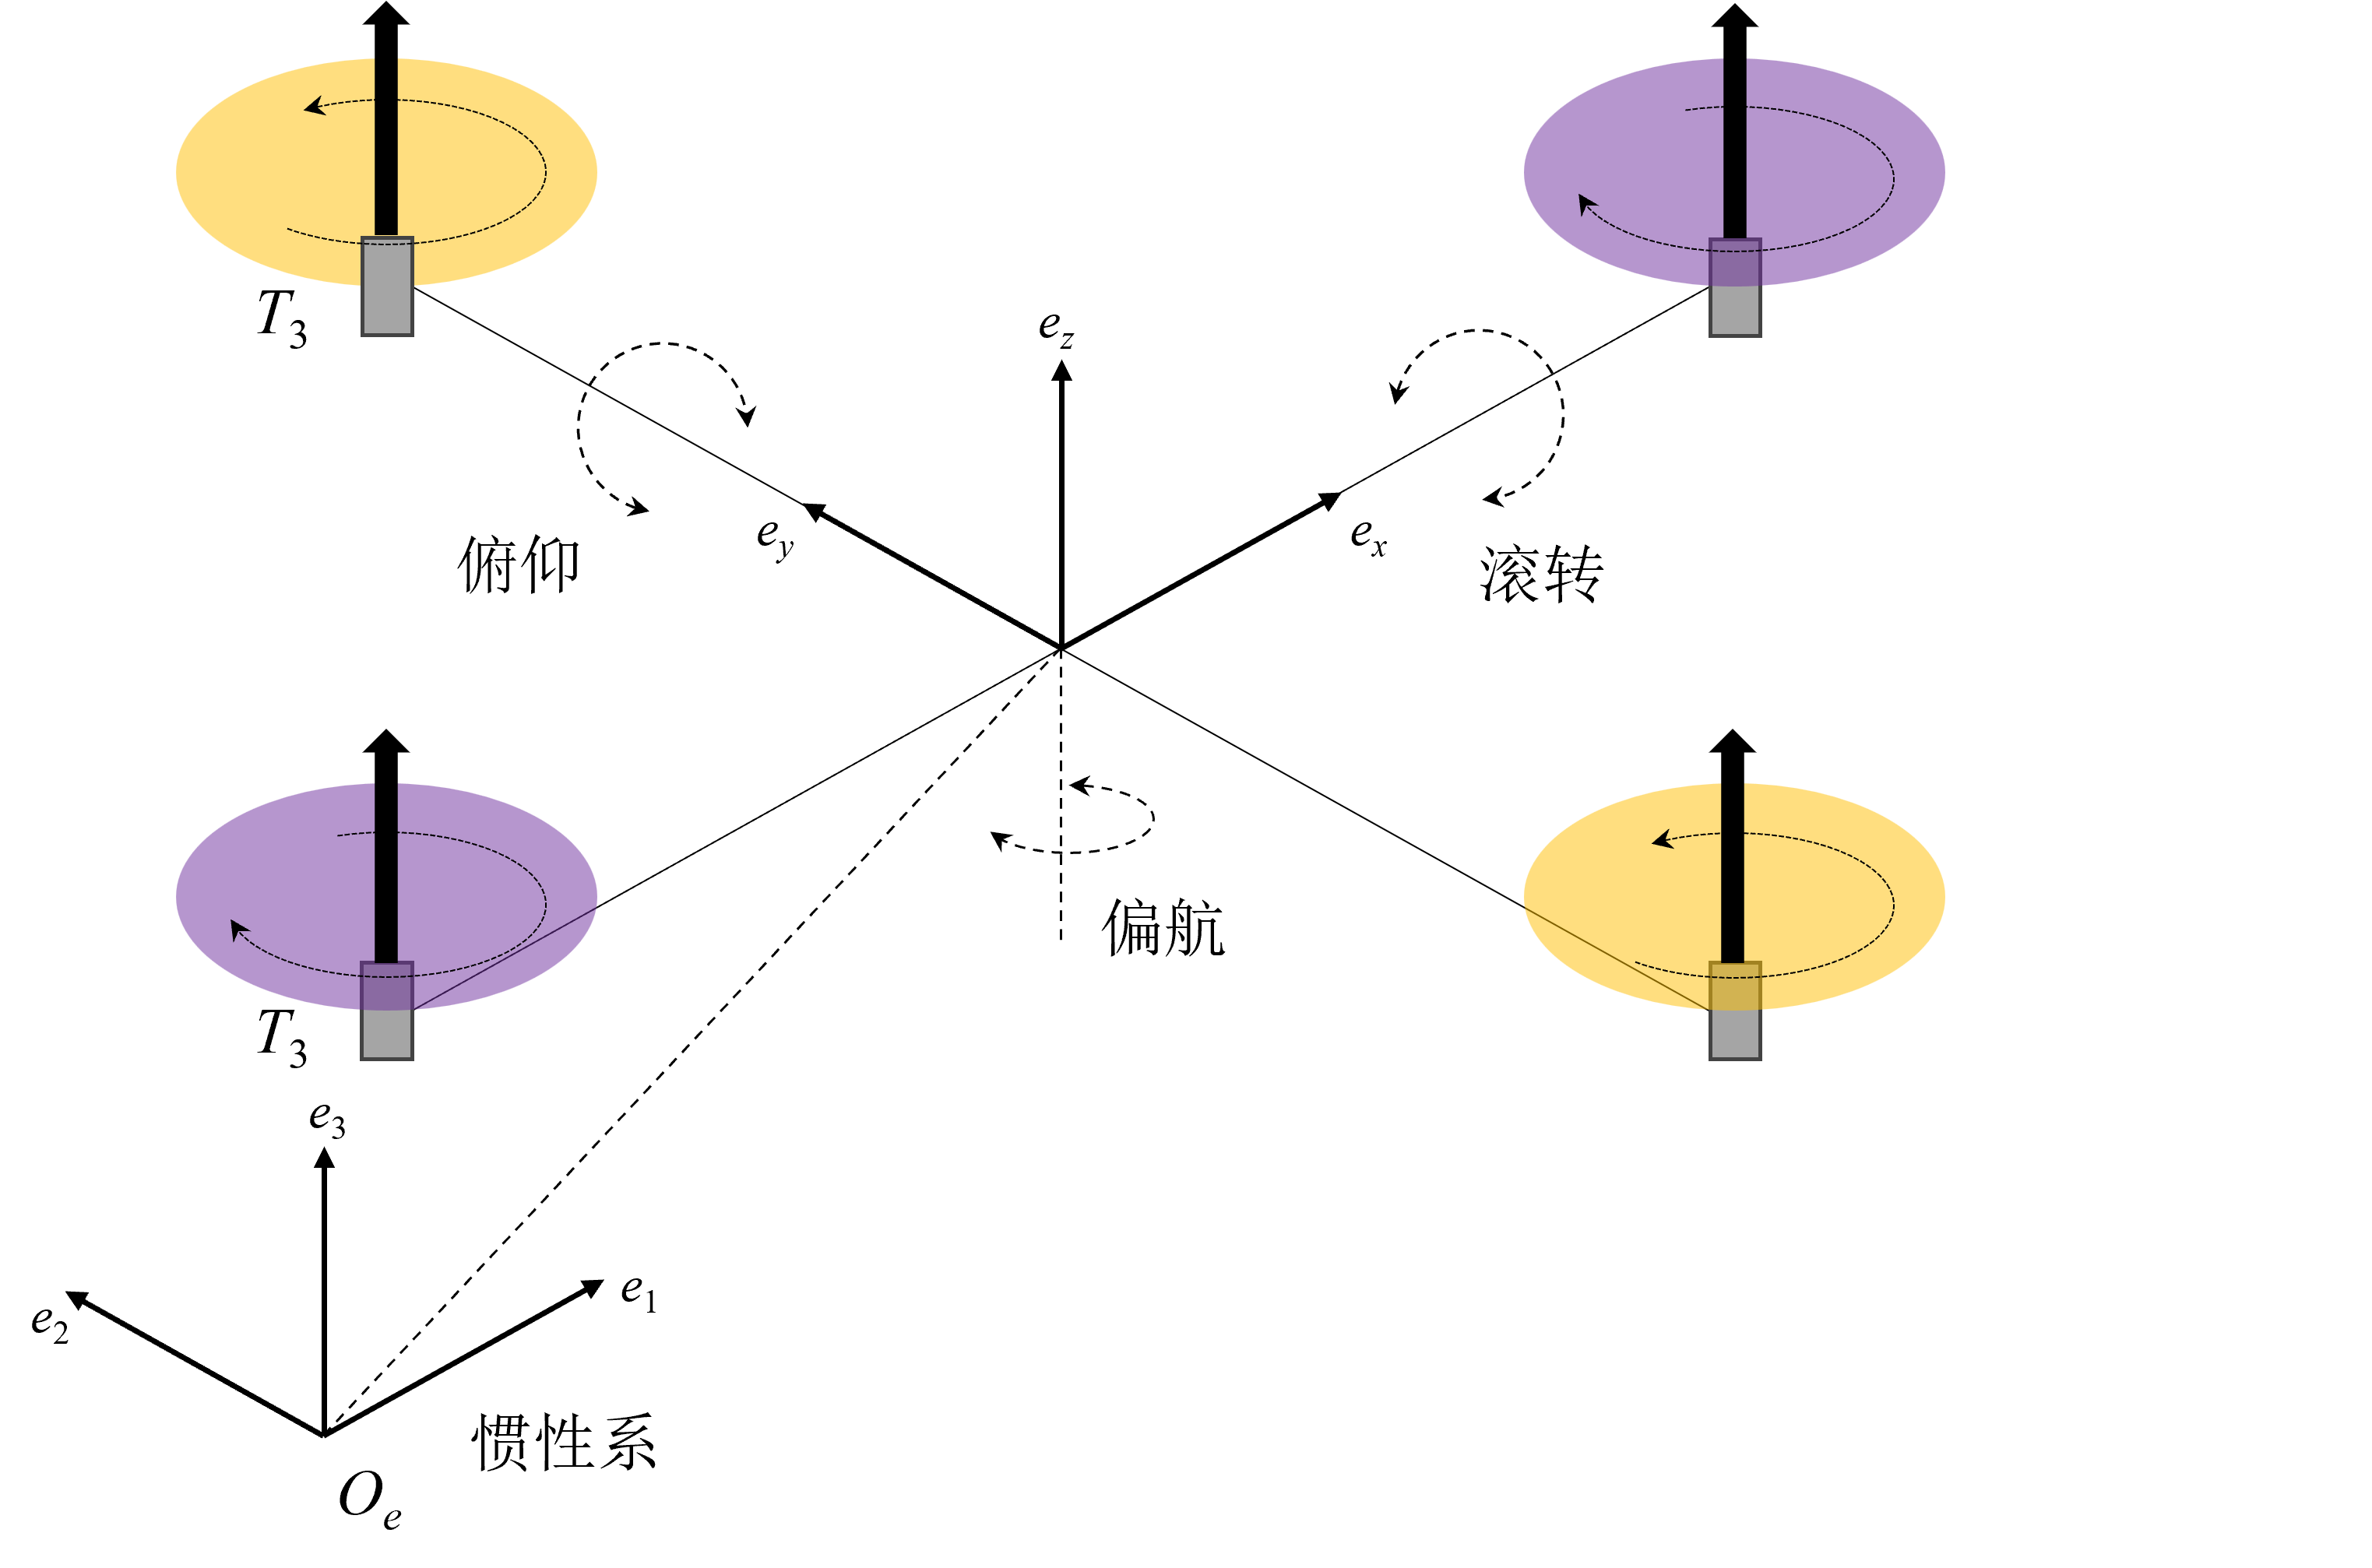
\includegraphics[width=28pc]{picture/2_1.png} 
	\caption{四旋翼无人机动力学结构} \label{2_1}
\end{figure}
% 要深入分析无人机绳系吊运系统的动力学特性,首先需要理解四旋翼无人机自身的动力学原理。四旋翼无人机是一种基于旋翼的飞行器,由四个旋翼推动飞行。为了平衡力矩,转子由两对对置的转子构成,一对正时针转动,一对反时针转动。四旋翼系统是高度非线性的,并且是一个欠驱动系统,有六个自由度和四个控制输入(即旋翼转速)。可以通过调整旋翼的转速来对四旋翼无人机进行控制,从而改变四旋翼无人机的力矩和推力特性。如图 \ref{2_1} 所示,四旋翼无人机设计为四个旋翼交叉共振。两个相对的旋翼沿同一方向旋转,通过改变旋翼的角速度可以控制四旋翼无人机的高度和位置。如果电机$T_1$、$T_2$、$T_3$和$T_4$产生的力矩相同,则四旋翼无人机可以保持平衡位置而不旋转。
四旋翼无人机的飞行控制主要依赖于调节四个电机 $T_1$ 、$T_2$ 、$T_3$ 和$T_4$ 的转速,从而实现不同方向的运动和姿态调整。其中,无人机的上升和下降通过同步增加或减少所有电机的转速来实现;滚转运动使无人机向左或向右倾斜,以便进行侧向移动;俯仰运动则通过前倾或后仰,使无人机向前或向后移动;偏航运动允许无人机在保持水平姿态的前提下,以顺时针或逆时针方向改变自身朝向。通过精确控制四个电机的转速组合,四旋翼无人机能够执行复杂的飞行动作,满足多种任务需求。
% 本章在分析四旋翼无人机动力学特性的基础上,建立了相应的数学模型,为后续章节中控制器的设计和实现提供了理论依据和数学支撑。

% 对于四旋翼无人机的上升和下降,可以通过同时增加或减小电机$T_1$、$T_2$、$T_3$和$T_4$的转速来实现;滚转是四旋翼无人机通过向左或向右倾斜,以允许侧向移动的运动;俯仰是指四旋翼无人机通过前倾或后仰,向前或向后运动;偏航是指在与地面保持水平的情况下,以顺时针或逆时针的方式改变四旋翼无人机的方向。四旋翼无人机通过控制四个电机的转速,可以完成不同的飞行作业。本章根据四旋翼无人机的动力学特性建立数学模型,为下面章节控制器的设计奠定基础。
\subsection{四旋翼无人机的坐标系}
为了便于建模和描述,首先引入两个右手直角坐标系的定义,并给出两个坐标系之间的转换关系。
\subsubsection{地面坐标系}
地面坐标系$o_ex_ey_ez_e$用于研究四旋翼无人机相对于地面的运动状态,确定机体的三维位置。一般来说,在地面坐标系中,常用的局部坐标系包括 NED(North-East-Down)坐标系和 ENU(East-North-Up)坐标系。NED 坐标系中,$o_ex_e$ 轴指向正北,$o_ey_e$ 轴指向正东,$o_ez_e$ 轴垂直地面向下;而 ENU 坐标系中,$o_ex_e$ 轴指向正东,$o_ey_e$ 轴指向正北,$o_ez_e$ 轴垂直地面向上,朝向天空的方向。
NED 坐标系更适用于飞行器和船舶等涉及垂直下降或沉降的系统,而 ENU 坐标系则因符合日常地理习惯,常见于地面交通、测量和定位任务。
本文使用NED坐标系,坐标原点选择在固连于地面的任意一点,确保动力学分析过程中具备统一且直观的参考基准。

\subsubsection{机体坐标系}
本文所采用的四旋翼无人机采用 “X” 型气动布局结构,使其在飞行过程中具备更高的灵活性和机动性。机体坐标系$o_bx_by_bz_b$固连于四旋翼无人机,其原点设在无人机的重心位置。$o_bx_b$ 轴位于无人机的对称平面内,指向机头方向,代表无人机前进的方向;$o_bz_b$ 轴同样位于无人机的对称平面内,并垂直指向下方,表示机体的垂直方向;$o_by_b$ 轴依据右手定则确定,与 $o_bx_b$ 和 $o_bz_b$ 轴垂直,形成完整的三维坐标系统。

\subsubsection{地面坐标系与机体坐标系之间的转换关系}
地面坐标系与机体坐标系之间的转换关系可以通过三个旋转矩阵来描述。具体来说,可以将地面坐标系依次沿机体坐标系进行旋转,即绕$z_b$轴旋转偏航角$\psi$,绕$y_b$旋转俯仰角$\theta$,绕$x_b$旋转滚转角$\phi$。对应的三个旋转矩阵$\boldsymbol{R}_\psi$、$\boldsymbol{R}_\theta$和$\boldsymbol{R}_\phi$分别为:
$$
\boldsymbol{R}_\psi=\begin{bmatrix}\cos\psi&-\sin\psi&0\\sin\psi&\cos\psi&0\\0&0&1\end{bmatrix} $$
$$	\boldsymbol{R}_\theta=\begin{bmatrix}\cos\theta&0&\sin\theta\\0&1&0\\-\sin\theta&0&\cos\theta\end{bmatrix} $$
$$\boldsymbol{R}_\phi=\begin{bmatrix}1&0&0\\0&\cos\phi&\sin\phi\\0&-\sin\phi&\cos\phi\end{bmatrix}
$$

通过上述三个旋转矩阵,任意矢量从地面坐标系转换到机体坐标系的转换矩阵可以表示为:
$$\begin{aligned}\boldsymbol{R}_{e-b}&=\boldsymbol{R}_{\psi}\boldsymbol{R}_{\theta}\boldsymbol{R}_{\phi}\\&=\begin{bmatrix}\cos\theta\cos\psi&\cos\theta\cos\psi&-\sin\theta\\\sin\phi\sin\theta\cos\psi-\cos\phi\sin\psi&\sin\phi\sin\theta\sin\psi+\cos\phi\cos\psi&\sin\phi\cos\theta\\\cos\phi\sin\theta\cos\psi+\sin\phi\sin\psi&\cos\phi\sin\theta\sin\psi-\sin\phi\cos\psi&\cos\phi\cos\theta\end{bmatrix}\end{aligned}$$

从机体坐标系到地面坐标系的转换矩阵表示为:
$$\begin{aligned}\boldsymbol{R}_{b-e}&=\bm{R}_{e-b}^\mathrm{T}\\&=\begin{bmatrix}\cos\theta\cos\psi&\sin\phi\sin\theta\cos\psi-\cos\phi\sin\psi&\cos\phi\sin\theta\cos\psi+\sin\phi\sin\psi\\\cos\theta\cos\psi&\sin\phi\sin\theta\sin\psi+\cos\phi\cos\psi&\cos\phi\sin\theta\sin\psi-\sin\phi\cos\psi\\-\sin\theta&\sin\phi\cos\theta&\cos\phi\cos\theta\end{bmatrix}\end{aligned}$$

\subsection{四旋翼无人机的模型}
四旋翼无人机模型通常分为运动学模型、动力学模型和控制效率模型三类。其中,
运动学模型不涉及质量和受力情况,而是专注于研究无人机速度对位置和姿态变化的影响;
% 该模型的输入变量是线速度和角速度,输出变量为无人机的位置信息和姿态角;
动力学模型涉及无人机的运动和受力情况,并与无人机的质量和转动惯量密切相关,主要用于分析外界受力对无人机运动速度的影响;
% ,该模型的输入变量是无人机旋翼产生的拉力和力矩,输出变量为无人机的速度和角速度;
控制效率模型用于描述螺旋桨转速与旋翼推力和力矩之间的关系,从而为动力学模型提供输入参数。
% 该模型的输入变量是螺旋桨的转速,输出变量为拉力和力矩,

在对无人机进行建模时,为了简化计算并确保模型的可行性,做出如下假设:

(1)无人机是刚体结构,没有内力,飞行时结构无形变;

(2)无人机的质量、螺旋桨阻力系数和转动惯量等基础参数默认不变;

(3)无人机总保持对称结构,其几何中心与重心位置一致。

运动学模型描述了无人机位置与速度以及速度和角速度之间的关系,其运动学方程可以表示为:
\begin{equation}
    \begin{aligned}
	\dot{\boldsymbol{p}}_e &= \boldsymbol{v}_e = \bm{R}_{b-e} \bm{v}_b \\
	\dot{\bm{\Theta}}_e &= \bm{W}_{b-e}  \bm{\omega}_b
\end{aligned}\label{2-1}
\end{equation}
其中,$\boldsymbol{p}_e=\left[x,y,z\right]^\mathrm{T}$为无人机在地面坐标系下的位置坐标,$\boldsymbol{v}_e=\left[v_{x},v_{y},v_{z}\right]^\mathrm{T}$为无人机在地面坐标系下的线速度,$\boldsymbol{v}_b=\left[u,v,w\right]^\mathrm{T}$为无人机在机体坐标系下的线速度,$\boldsymbol{R}_{b-e}$为上一小节定义的转换矩阵,$\bm{\Theta}_e=\left[\phi,\theta,\psi\right]^\mathrm{T}$为无人机在地面坐标系下的姿态角度,$\bm{W}_{b-e}$为地面坐标系下欧拉角速度变换到机体旋转角速度的旋转矩阵,$\boldsymbol{\omega}_b=\left[{\omega}_{b_x},{\omega}_{b_y},{\omega}_{b_z}\right]^\mathrm{T}$ 为无人机机体坐标系下的角速度,姿态旋转矩阵具体形式如式(\ref{2-2})所示:
\begin{equation}
	\boldsymbol{\omega}_b=\begin{bmatrix}\omega_{xb}\\\omega_{yb}\\\omega_{zb}\end{bmatrix}=\begin{bmatrix}1&0&-\sin\theta\\0&\cos\phi&\cos\theta\sin\phi\\0&-\sin\phi&\cos\theta\cos\phi\end{bmatrix}\begin{bmatrix}\dot\phi\\\dot\theta\\\dot\psi\end{bmatrix}
	\label{2-2}
\end{equation}

通常情况下,无人机在飞行过程中其姿态角的变化范围较小,可以近似认为有下式成立:
\begin{equation}
	\boldsymbol{\omega}_b=\begin{bmatrix}{\omega}_x\\{\omega}_y\\{\omega}_z\end{bmatrix}=\begin{bmatrix}\dot{\phi}\\\dot{\theta}\\\dot{\psi}\end{bmatrix}
	\label{2-3}
\end{equation}

以上详细描述了四旋翼无人机系统的运动学模型以及其在不同坐标系下的位置与线速度、角度与角速度之间的转换关系。接下来,将对无人机的动力学模型进行研究。无人机整体可视为一个刚体,其运动可分为平移运动和旋转运动两部分。平移运动基于牛顿法进行分析,旋转运动则通过欧拉法进行分析,从而构建其动力学模型。无人机动力学的基本方程如式(\ref{2-4})所示:
\begin{equation}
	\begin{aligned}
		m\dot{\boldsymbol{v}}_e&=mg\bm{e}_{3}-\boldsymbol{R}_{b-e}f\bm{e}_{3}\\
		\boldsymbol{J}\dot{\boldsymbol{\omega}_b}&=-\bm \omega_b \times \bm J \bm \omega_b+\boldsymbol{\tau}
	\end{aligned}\label{2-4}
\end{equation}
其中$m$为无人机的质量,$g\in\mathbb{R}^+$为重力加速度,$\bm{e_{3}}=\left[0,0,1\right]^\mathrm{T}$,$\boldsymbol{\tau}=\left[\tau_x,\tau_y,\tau_z\right]^\mathrm{T}$表示无人机四个螺旋桨产生的力矩,$\boldsymbol{J}$为无人机的惯量矩阵,$f\in\mathbb{R}^+\cup\{0\}$表示无人机螺旋桨总拉力的大小,该拉力是单向的,其形式如式 (\ref{2-5})所示:
\begin{equation}
	f=\sum_{i=1}^4f_i=c_\mathrm{T}\Omega_i^2
	\label{2-5}
\end{equation}
其中$f_i$表示表示一个旋翼在机体坐标系下旋转产生的升力,与旋翼的转速的平方正相关。$c_\mathrm{T}=1/4\pi^2\cdot\rho D_\mathrm{p}^4C_\mathrm{T}$为螺旋桨的升力系数,其大小与无人机自身的材质、倾斜角等因素有关,$\Omega_i$为
单个螺旋浆的转速。由于本文采用 “X” 型气动布局,其实际力臂长度为机臂长度的$\sqrt{2}/2$倍。因此,无人机每个螺旋桨所产生的力矩如式(\ref{2-6})所示:
\begin{equation}
	\left\{ \begin{array}{l}
		\tau_x={\sqrt{2}}/{2}dc_\mathrm{T}\left(\Omega_1-\Omega_2-\Omega_3+\Omega_4\right)\\
		\tau_y={\sqrt{2}}/{2}dc_\mathrm{T}\left(\Omega_1+\Omega_2-\Omega_3-\Omega_4\right)\\
		\tau_z=c_\mathrm{M}\left(\Omega_1-\Omega_2+\Omega_3-\Omega_4\right)\\
	\end{array} \right.
		\label{2-6}
\end{equation}
其中$c_M$为螺旋桨的反扭力系数,其产生的力矩方向沿$z$轴方向。$d\in\mathbb{R}^+$为无人机重心和任一电机转动轴线之间的距离。为了能够对应控制器中的控制量,定义虚拟控制变量为$\bm{U}=\left[U_1,U_2,U_3,U_4\right]^\mathrm{T}=\left[f,\tau_x,\tau_y,\tau_z\right]^\mathrm{T}$,那么,将式(\ref{2-2})、(\ref{2-3})、(\ref{2-5})、(\ref{2-6})代入式(\ref{2-1})和(\ref{2-4})中,即可得到四旋翼无人机的控制模型:
\begin{equation}
		\left\{
	\begin{aligned}
		&\dot{x}=v_{x}\\
		&\dot{y}=v_{y}\\
		&\dot{z}=v_{z}\\
		&\ddot{x}=\frac{U_{1}}{m}\left(\cos\phi\cos\psi\sin\theta+\sin\phi\sin\psi\right)\\
		&\ddot{y}=\frac{U_{1}}{m}\left(\cos\phi\sin\psi\sin\theta-\cos\psi\sin\phi\right)\\
		&\ddot{z}=\frac{U_{1}}{m}\left(\cos\phi\cos\theta\right)-g\\
		&\dot{\phi}={\omega}_x+\tan\theta\left({\omega}_y\sin\phi+{\omega}_z\cos\phi\right)\\
		&\dot{\theta}={\omega}_y\cos\phi-{\omega}_z\sin\phi\\
		&\dot{\psi}=\frac{{\omega}_y\sin\phi+{\omega}_z\cos\phi}{\cos\theta}\\
		&\ddot{\phi}=\frac{(I_{y}-I_{z})\cdot \dot{\theta}\dot{\psi}+U_{2}}{I_{x}}\\
		&\ddot{\theta}=\frac{(I_{z}-I_{x})\cdot \dot{\phi}\dot{\psi}+U_{3}}{I_{y}}\\
		&\ddot{\psi}=\frac{(I_{x}-I_{y})\cdot \dot{\phi}\dot{\theta}+U_{4}}{I_{z}}\end{aligned}
	\right.
	\label{2-7}
\end{equation}

\section{单无人机绳系吊运系统的数学模型}
四旋翼无人机绳系吊运系统是一个复杂的飞行控制系统。在吊装运输场景中,无人机在满足自身飞行需求的同时,还受到吊装载荷施加的拉力干扰。单无人机吊装载荷受力分析如图 \ref{2_2} 所示,其中$F$表示无人机产生的升力,$G$表示无人机自身的重力,$G_0$表示吊挂载荷的重力,$T$表示载荷对无人机施加的拉力,$\theta$表示系绳与垂直平面之间的夹角。

\begin{figure}[hbt!]
	\centering
	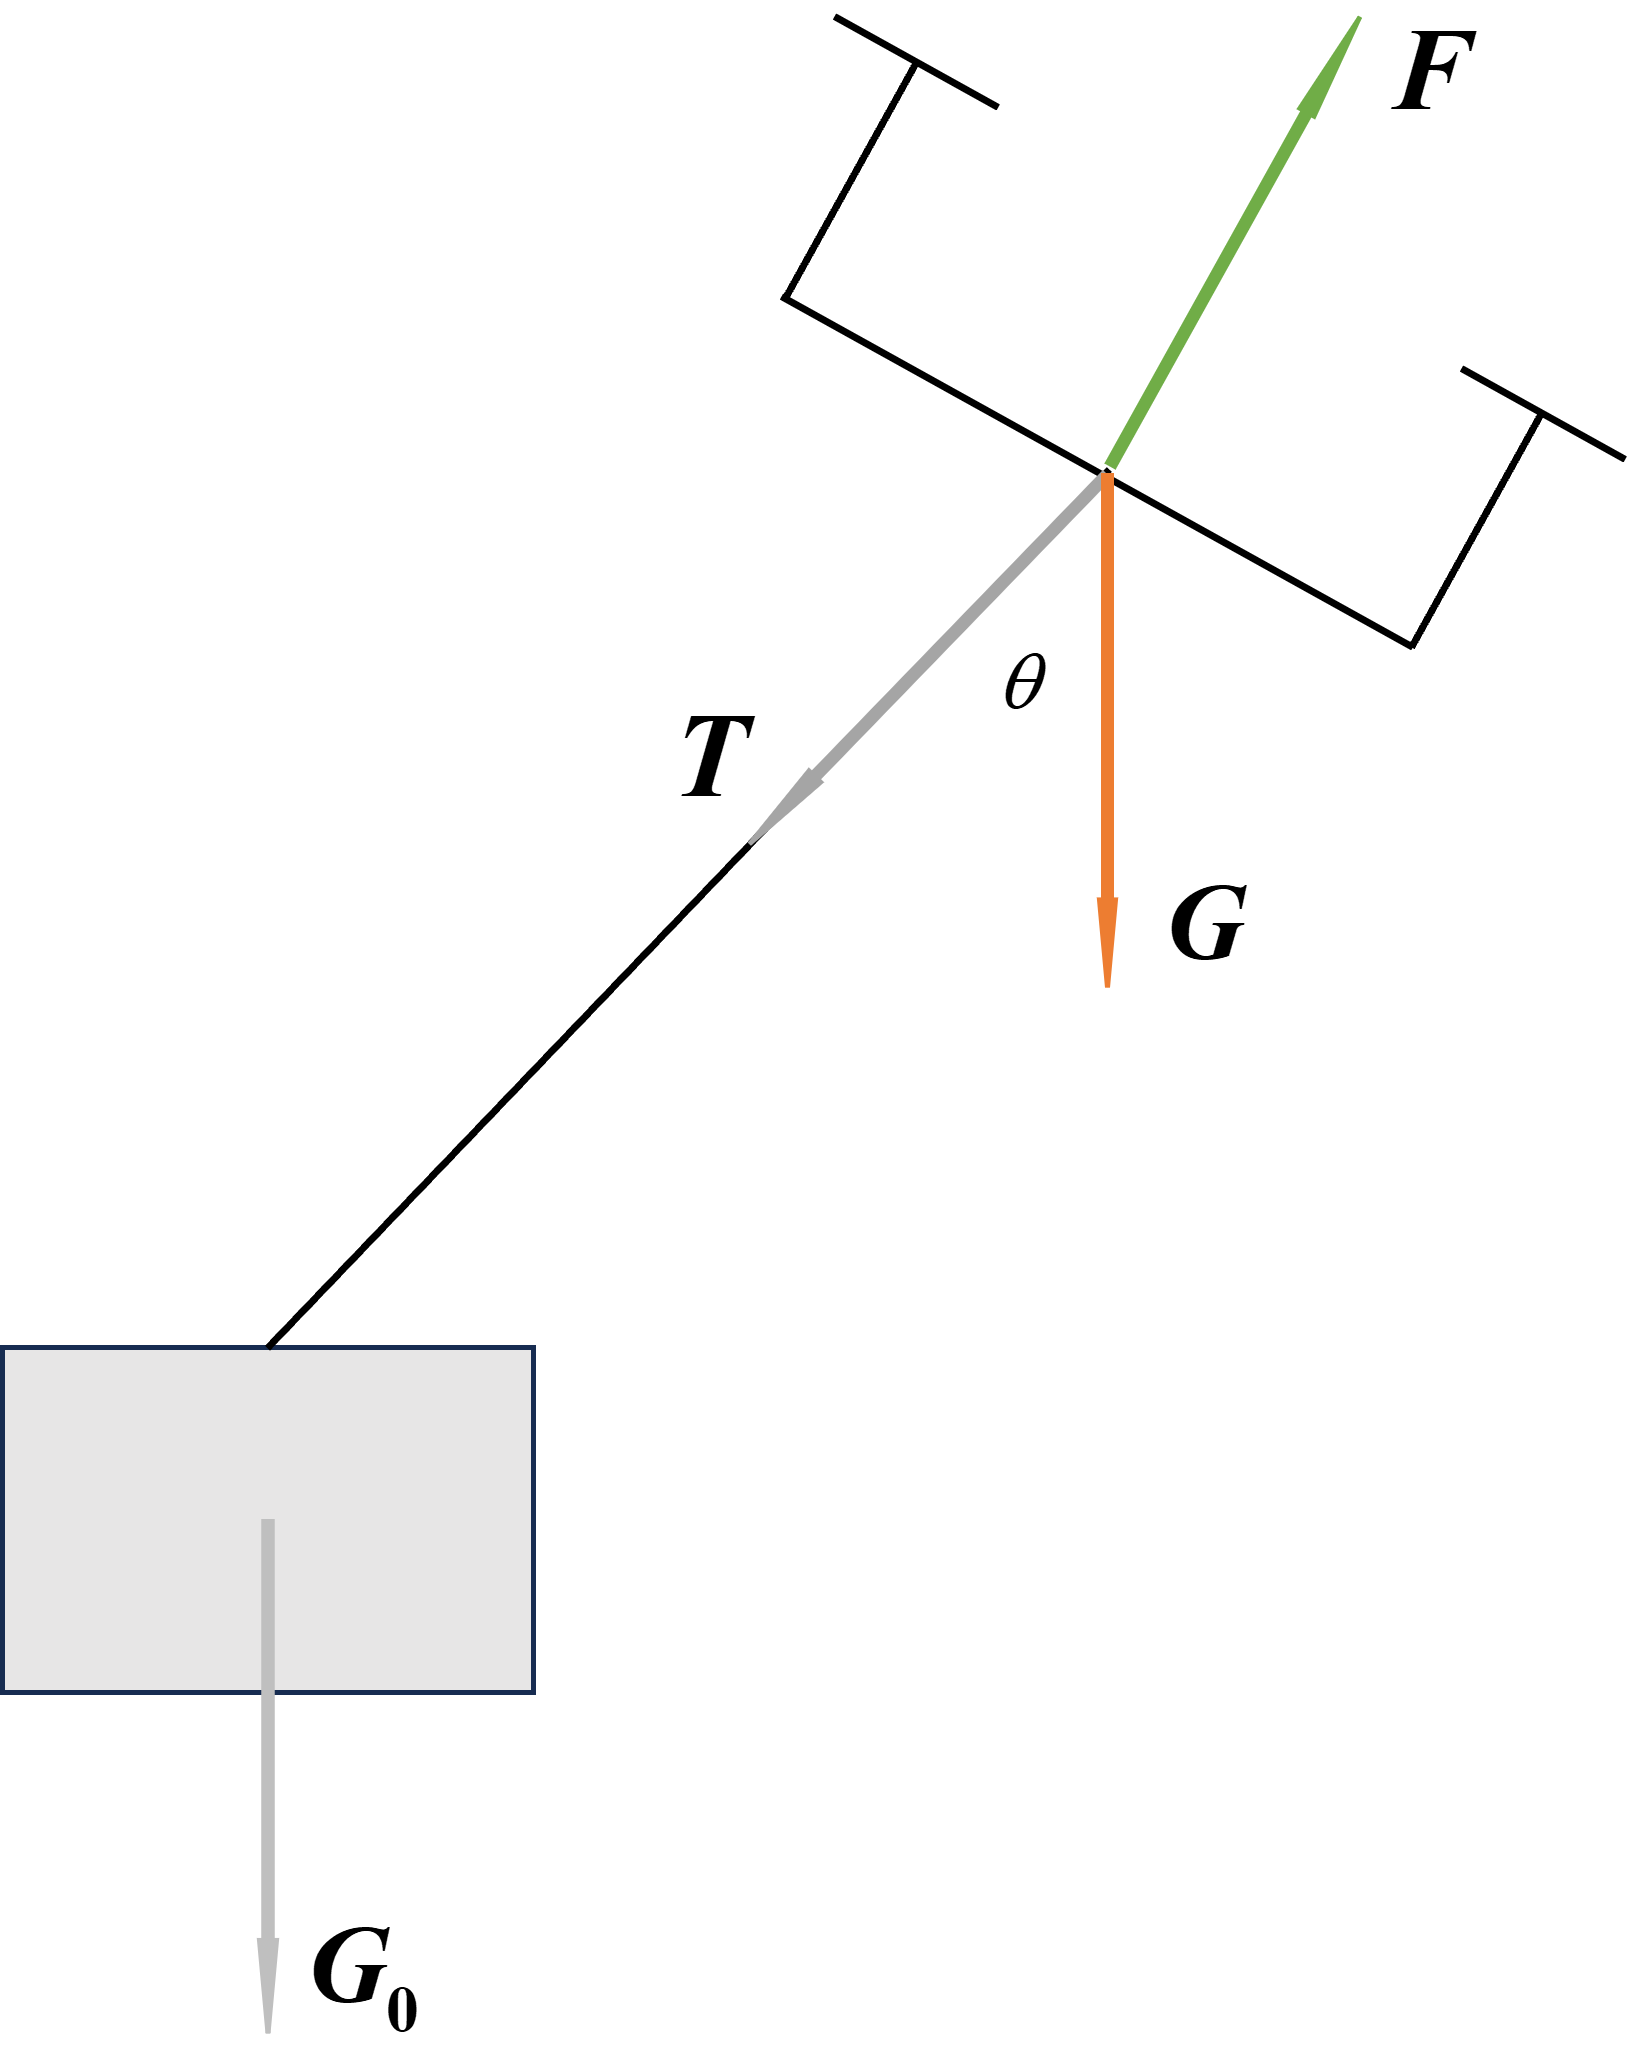
\includegraphics[width=16pc]{picture/2_2.png} 
	\caption{单无人机吊装载荷受力分析} 
	\label{2_2}
\end{figure}
对于无人机绳系吊运系统来说,在轨迹跟踪时其系绳并不一定总是保持绷直状态的,在无人机的高速移动中系绳上的拉力可能为零。因此,本文建立无人机绳系吊运系统的混合模型,考虑系绳上的拉力不为零和拉力为零这两种情况。

\subsection{系绳拉力不为零时的模型}

无人机绳系吊运系统由载荷相对于地面坐标系的位置、载荷姿态和无人机的姿态来定义。当系绳拉紧时,该系统具有八个自由度,并存在四个自由度的欠驱动。无人机和载荷的位置之间的关系为:
\begin{equation}
	\bm p_q=\bm p_l-l\bm q
	\label{2-8}
\end{equation}
其中$\bm p_q$、$\bm p_l$分别为无人机和载荷的位置,$l$为系绳的长度,$\bm q$表示从无人机质心指向载荷质心的单位向量。本文采用拉格朗日法来推导运动方程。系统的拉氏量 $\mathcal{L}:T\bar{Q}\to\mathbb{R}$ 定义为$\mathcal{L}=\mathcal{T}-\mathcal{U}$,其中$\mathcal{T}:TQ\to\mathbb{R}$和${\mathcal{U}}:Q\to\mathbb{R}$分别是机械系统的动能和势能,它们的定义如下:
\begin{equation}
\begin{aligned}
	\mathcal{T}=\frac{1}{2}&m_{q}\bm v_{q} \bm v_{q}+\frac{1}{2}m_{l}\bm v_{l} \bm v_{l}+\frac{1}{2}\langle\hat{\bm  \omega_q},\widehat{\bm J_{q}\bm  \omega_q}\rangle\\
	&\mathcal{U}=m_{q}g\bm e_{3} \bm x_{Q}+m_{l}g\bm e_{3} \bm x_{l}
\end{aligned}
	\label{2-9}
\end{equation}
其中$\bm v_q$、$\bm v_l$分别为无人机和载荷的速度,$m_q$、$m_l$分别为无人机和载荷的质量,$\langle\cdot,\cdot\rangle $表示内积,$\hat{.}$被定义为使得 $\hat{\bm x}\bm y=\bm x\times \bm y$对于所有$\bm x,\bm y\in\mathbb{R}^3$恒成立,$\omega_q$为无人机在机体坐标系下的角速度。在本文中,$\lambda_m(\cdot)$和 $\lambda_n(\cdot)$ 分别表示矩阵的最小和最大特征值。系统的动力学满足拉格朗日原理:
\begin{equation}
	\bm \delta\int_0^\tau\mathcal{L} \text{dt}+\int_0^\tau\left(\langle \bm W_1,\hat{\bm \tau}\rangle+\bm W_2 f\bm{R}_{b-e}\bm e_3\right) \text{dt}=0
	\label{2-10}
\end{equation}
其中$\bm W_{1}=\bm R_{b-e}^\mathrm{T}\bm \delta \bm R_{b-e}$是定义在旋转空间上的变分向量场, $ \bm W_{2}=\bm \delta \bm x_{Q}=\bm \delta \bm x_{L}-l\bm \delta q$是定义在平移空间上的变分向量场,两者共同描述刚体系统中的变分动态,并且满足以下条件:
\begin{equation}
	\begin{aligned}
	&\bm \delta \bm q = \bm \xi \times \bm q\\
	\bm \delta \dot{\bm q} = &\dot{\bm \xi} \times \bm q + \bm \xi \times \dot{\bm q} \\
	\bm \delta\bm  R&_{b-e} = \bm R_{b-e} \hat{\bm \eta} \\
	\bm \delta \hat{\bm  \omega _q}& = \widehat{\hat{\bm  \omega_q} \bm \eta} + \hat{\dot{\bm \eta}}
\end{aligned}
\end{equation}
其中$\bm \delta \bm q$为二维球面上的变分,$\bm \delta \bm R$为三维空间上的变分。
向量 $\bm{\xi} \in \mathbb{R}^3$ 是一个三维实数向量,满足 $\bm{\xi}$ 与向量 $\bm{q}$ 的点积为零,即$\bm{\xi}$ 垂直于 $\bm{q}$,向量 $\bm{\eta} \in \mathbb{R}^3$ 是一个三维实数向量。

由于式(\ref{2-10})对所有可能的变化都是满足的,因此得到带有系绳载荷的无人机的运动方程为:
\begin{equation}
	\begin{aligned}
		&\dot{\bm x}_{l}=\bm v_{l} \\
		(m_q+m_l)(\dot{\bm v}_L+g\bm e_3)& =(\bm q f\bm R\bm e_3-m_Ql(\dot{\bm q}\dot{\bm q}))\bm q \\
		&\dot{\bm q}=\bm \omega_l\times \bm q \\
		m_{q}l \dot{\bm \omega_l}&=-\bm q\times f\bm R\bm e_{3} \\
		&\dot{\bm R_{b-e}}=\bm R_{b-e}\hat{\bm  \omega_q} \\
		\bm J_{q}\dot{\bm  \omega_q}+&\bm  \omega_q\times \bm J_{q}\bm  \omega_q=\bm \tau
	\end{aligned}
\end{equation}

上述动力学可以写成标准形式 $\dot{\bm X}_n= f_n(\bm X_n)+g_n(\bm X_n)\bm u$ ,其中 $\bm X_n = \{\bm x_l,\bm q,\bm R_{b-e},\bm v_l,\bm \omega_l,\bm \omega_q\}$ 是系统的状态,$\bm u = \left[f,\bm \tau \right]$是系统的输入。
\subsection{系绳拉力为零时的模型}
当系绳拉力趋于零时,无人机和吊挂载荷作为独立系统,载荷处于自由落体状态。在这种情况下,无人机绳系吊运系统的运动方程为:
\begin{equation}
	\begin{aligned}
	&\dot{\bm x}_{l}=\bm v_{l}\\
	\quad m_{l}(&\dot{\bm v}_{l}+g\bm e_{3})=0\\
	&\dot{\bm x}_{q}=\bm v_{q}\\
	\quad m_{q}(\dot{\bm v}_{q}&+g\bm e_{3})=f\bm R_{b-e}\bm e_{3}\\
	&\dot{\bm R_{b-e}}=\bm R_{b-e}\hat{\omega_q}\\
	\quad \bm J_{q}\dot{\bm \omega_q}+&\bm \omega_q \times \bm J_{q}\bm \omega_q=\bm \tau
\end{aligned}
\end{equation}

上述方程可以写成标准形式$\dot{\bm X}_z=f_z(\bm X_z)+\ g_z(\bm X_z)\bm u$,$\bm X_z = \{\bm x_L,\bm x_q,\bm R_{b-e},\bm v_l,\bm v_q,\bm \omega_b\}$为状态。

\subsection{混合系统的模型}
系绳吊挂载荷的无人机系统为一个混合系统。其动力学会在两种不同的状态之间切换,具体来说,当系绳中的拉力降为零时,系统进入松弛状态,而当拉力恢复时,松弛的系绳被拉紧,系统进入拉伸状态。这种切换导致系统的动力学发生变化。因此,混合系统的数学模型可表示为:
\begin{equation}
	\left.\begin{aligned}&\Sigma_{n}:\left\{\begin{array}{ll}\dot{\bm X_n}= f_n(\bm X_n)+ g_n(\bm X_n)\bm u  &\bm X_n\notin \mathbb{S}_z\\\bm X_z^+=\Delta_{n\to z}(\bm X_n^-)  &\bm X_n\in \mathbb{S}_z\end{array}\right.\\&\Sigma_{z}:\left\{\begin{array}{ll}\dot{\bm X_z}=f_z(\bm X_z) + g_z(\bm X_z)\bm u \ \ &\bm X_z\notin \mathbb{S}_n\\\bm X_n^+=\Delta_{z\to n}(\bm X_z^-) \ &\bm X_z\in \mathbb{S}_n\end{array}\right.\end{aligned}\right.
	\label{eq:混合模型}
\end{equation}
其中集合$\mathbb S_z = \{ \bm X_n \mid  T \equiv 0 \}$,$\mathbb S_n = \{ \bm X_z \mid \|\bm x_Q - \bm x_L\| \equiv l, d \|\bm x_Q - \bm x_L\| /\text{dt}> 0 \}$,系绳上的拉力定义为$ T = \|m_L (\ddot{\bm x}_L + g\bm{e}_3)\|$,状态转移映射$\Delta_{n\to z}$为单位映射,$\Delta_{z\to n}$为两个物体非弹性碰撞的模拟,并满足条件$\dot{\bm x}_Q^+-\dot{\bm x}_L^+=0$。

\section{多无人机绳系吊运系统的数学模型}
由于单个无人机的承载能力有限,提出了一种多无人机协同吊装运输方案,以显著提升系统的承载能力。当无人机数量$n\geq3$时,多架无人机可以协同对载荷进行精准控制\cite{fink2011planning}。本文研究由3架规格型号相同的无人机协同运输吊挂载荷的问题。该吊运系统由三架无人机、三根系绳和被运输的载荷组成。三架无人机协同吊装运输载荷的示意图如图 \ref{2_3} 所示,每架无人机分别用$q_1$、$q_2$、$q_3$表示,吊挂载荷用$l$表示,三架无人机保持相同水平高度,且相对间距为$d$。
\begin{figure}[hbt!]
	\centering
	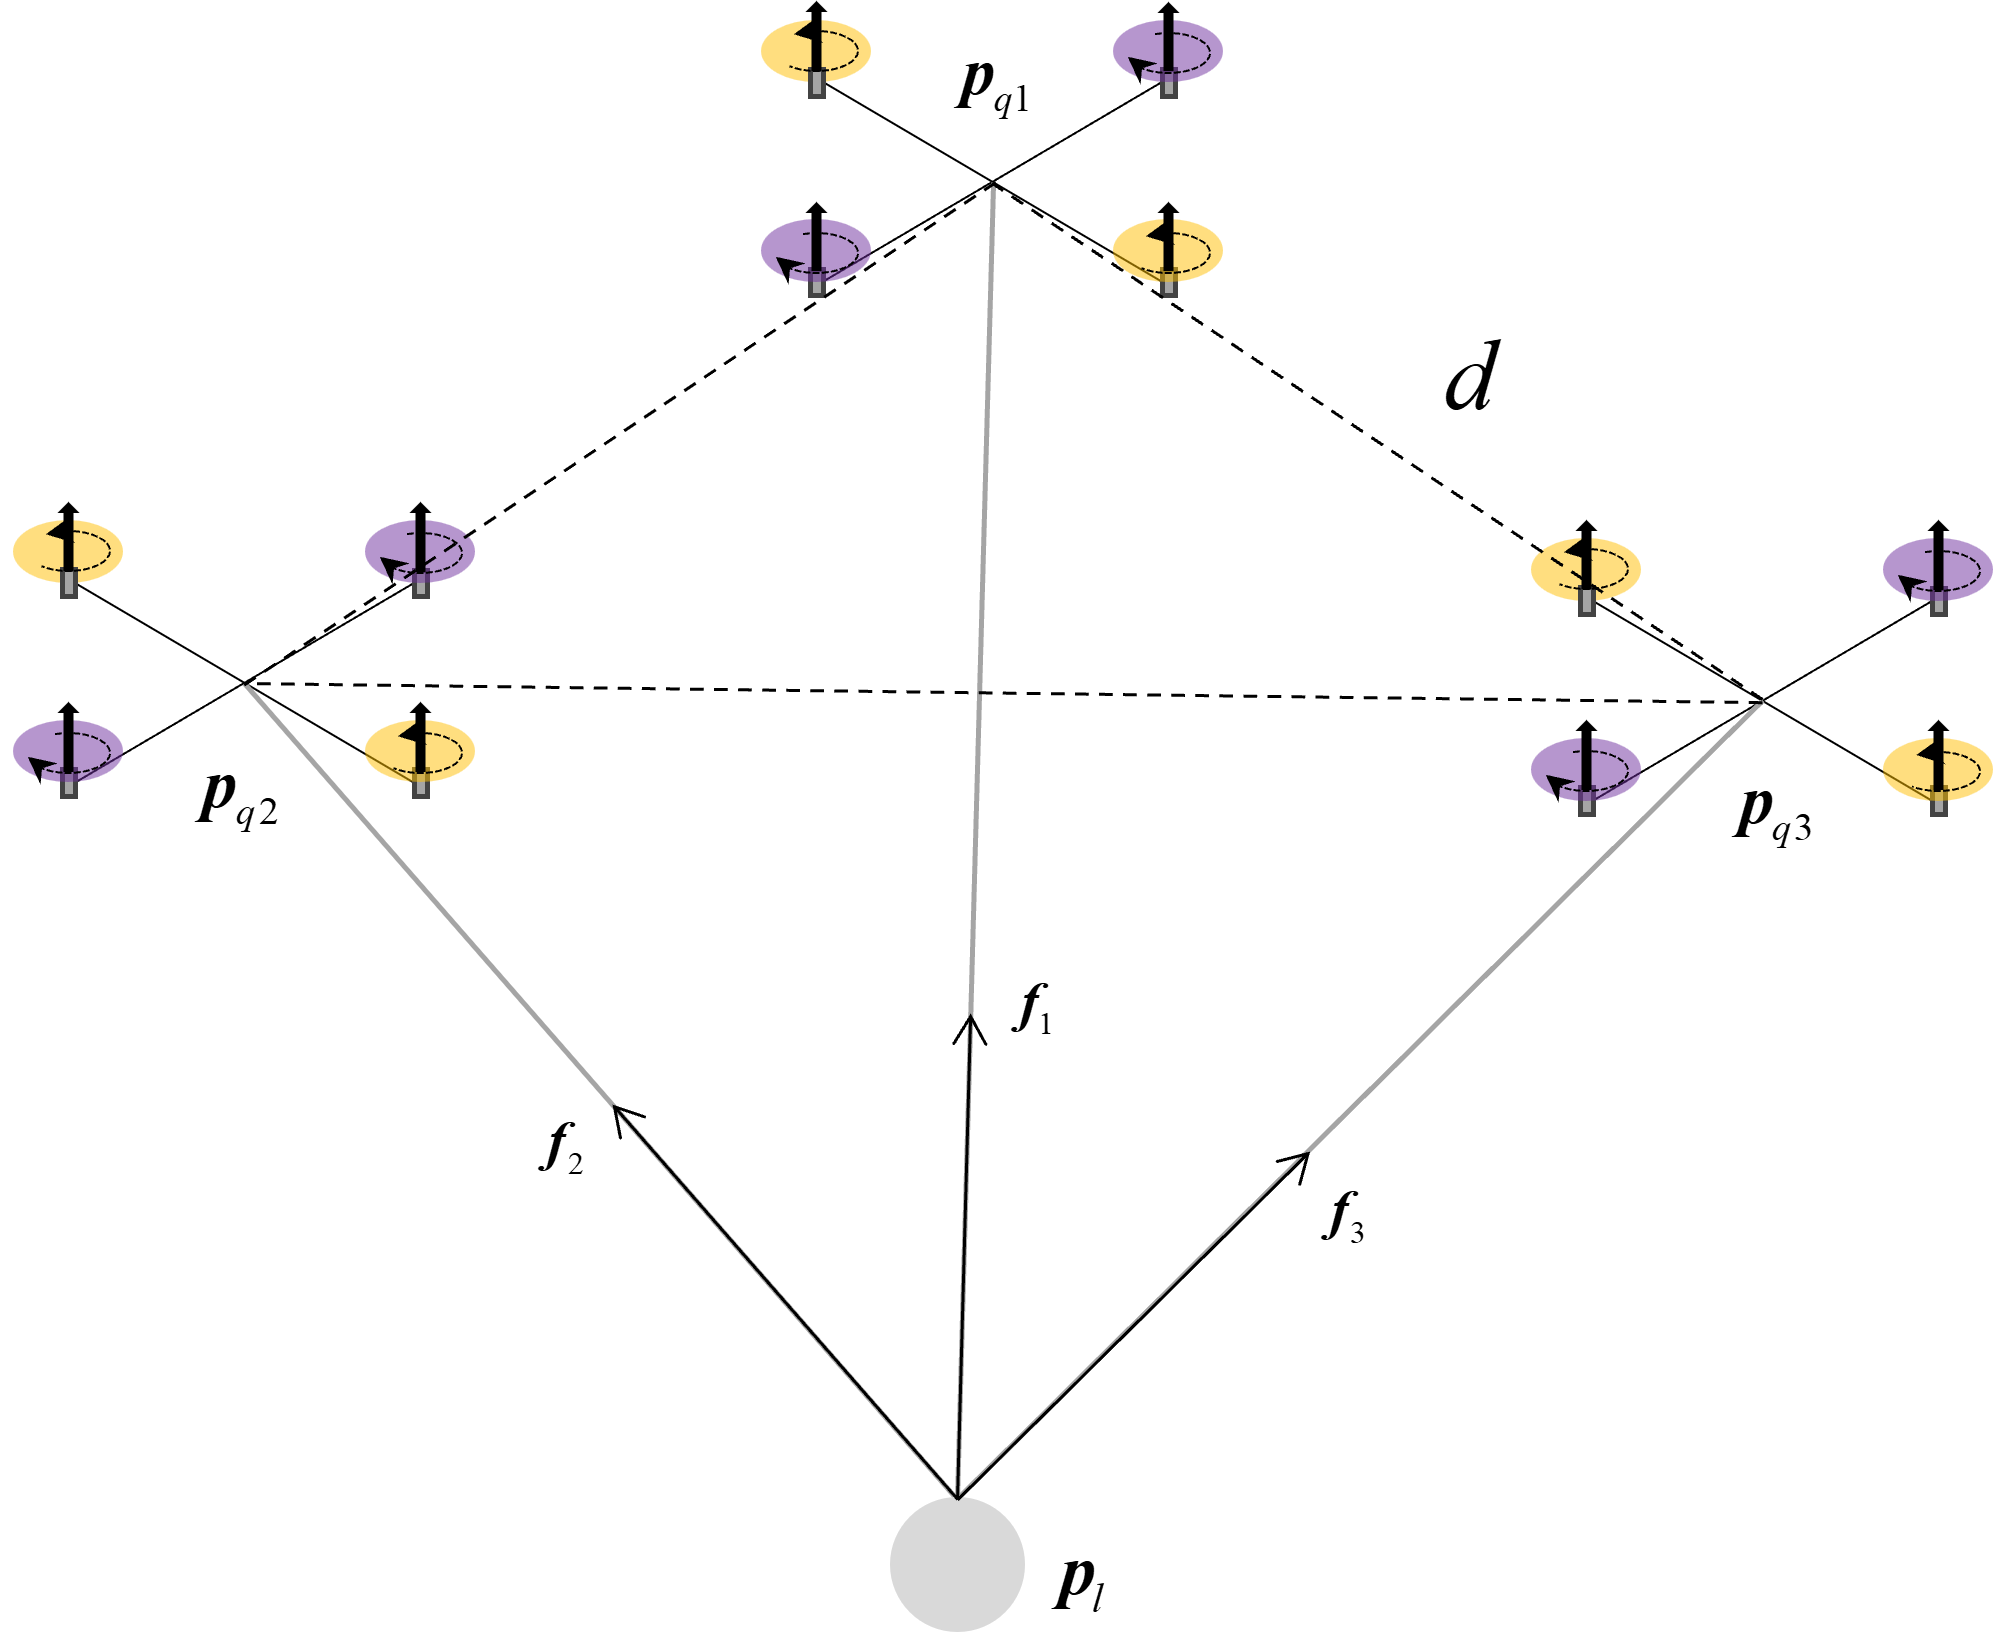
\includegraphics[width=28pc]{picture/2_3.png} 
	\caption{多无人机吊运系统} \label{2_3}
\end{figure}
在推导多无人机绳系吊运系统的数学模型之前,先做了如下假设:

(1)无人机绳系吊运系统所吊挂的载荷被视为刚体; 

(2)连接无人机与有效载荷之间的系绳没有质量,且不会发生缠绕;

(3)所有系绳都连接在无人机的质心处,系绳的牵引力能够影响无人机的平动,但是不影响无人机的转动。 

基于上述假设,本小节将建立多无人机绳系吊运系统的数学模型。


在地面坐标系下,载荷位置向量为$\bm p_{l}=[p_{lx},p_{ly},p_{lz}]^{\mathrm{T}}$,三架无人机的位置向
量分别为$\bm p_{q_1}$、$\bm p_{q_2}$、$\bm p_{q_3}$,系绳长度为$l$。对吊挂的载荷进行受力分析,由牛顿第二定律可得出:
\begin{equation}
	\label{2-15}
	\begin{aligned}
		&\bm f_{i}=\frac{1}{l}(\bm p_{q_i}-\bm p_{l})T_{i} \\
		&m_{1}\ddot{\bm p}_{1}=-m_{1}g\bm e_{3}+\sum_{i=1}^{3}\bm f_{i}
	\end{aligned}
\end{equation}
其中$\bm f_{i}$表示第$i$根系绳在惯性坐标系下所提供的拉力向量;$T_{i}$表示第$i$根系绳提供的拉力值标量。

在该系统中,$\alpha_{i}$和$\beta_i$分别描述了系绳在地面坐标系下相对于吊挂载荷的偏角。从载荷质心指向无人机质心的单位方向向量表示为:
\begin{equation}
	\boldsymbol{q}_i=\left[\cos\alpha_i\cos\beta_i,\sin\alpha_i\cos\beta_i\,\sin\beta_i\right]^\mathrm T
\end{equation}

在实际过程中,吊挂载荷始终位于三架无人机之间,$\alpha_{i}$和$\beta_i$满足条件:
$0^\circ\leq\alpha_i\leq360^\circ$,$0^\circ\leq\beta_i\leq90^\circ$。考虑到无人机在飞行过程中可能存在碰撞风险,实际的$\beta_i$应限制在更小的合理范围内。

类似\autoref{2-8},在确定吊挂载荷位置后,可进一步确定三架无人机的位置:
\begin{equation}
\begin{aligned}
	\boldsymbol{p}_{l}=&\left[p_{l_{x}},p_{l_{y}},p_{l_{z}}\right]^{\mathrm{T}} \\
	\boldsymbol{p}_{q_1}&=\boldsymbol{p}_l+l\boldsymbol{q}_1 \\
	\boldsymbol{p}_{q_2}&=\boldsymbol{p}_{l}+l\boldsymbol{q}_{2} \\
	\boldsymbol{p}_{q_3}&=\boldsymbol{p}_l+l\boldsymbol{q}_3
\end{aligned}
\end{equation}
% 上式中,$\bm{p}_{q_1}$,$\bm{p}_{q_2}$,$\bm{p}_{q_3}$和$\bm{p}_l$分别表示三架无人机和吊挂载荷的位置,$l$是系
% 绳长度。

依照前述分析,无人机的控制输入为$\bm{U}=\left[U_1,U_2,U_3,U_4\right]^\mathrm{T}=\left[f_i,\tau_{x_i},\tau_{y_i},\tau_{z_i}\right]^\mathrm{T}$,其中$f_{i}$,$\tau_{x_i}$,$\tau_{y_i}$,$\tau_{z_i}$表示第 $i$ 个无人机的控制力和控制力矩大小,具体形式参见式(\ref{2-5})和(\ref{2-6})。
同时,为了模拟系统受到的未知扰动,在系统中直接施加一个外界干扰力$\bm f_w=\left[f_{x_w},f_{y_w},f_{z_w}\right]^\mathrm{T}$以表征诸如无人机诱导气流等外部因素的影响。

在三架无人机绳系吊挂载荷系统中,存在三个非零拉力系绳产生的完整约束,不考虑载荷的刚体转动情况下,整个系统自由度为18(6×3+3-3)。为方便后续多机吊挂研究,选择吊挂载荷的位置,三架无人机的姿态角以及三根系绳与吊挂载荷形成的偏离角度作为系统的广义坐标,记作:
\begin{equation}
	\boldsymbol{X}_n=\left[
	p_{l_x} , p_{l_y} , p_{l_z},\alpha_1,\beta_1,\phi_1,\theta_1,\psi_1,\alpha_2,\beta_2,\phi_2,\theta_2,\psi_2,\alpha_3,\beta_3,\phi_3,\theta_3,\psi_3
	\right]^\mathrm T
\end{equation}

类似式(\ref{2-9}),三架无人机吊挂载荷系统的动能和势能分别表示如下:
\begin{equation}
	\begin{aligned}
	\mathcal{T}=\frac{1}{2}m_{l}{\boldsymbol{v}}_{l}^\mathrm{T}{\boldsymbol{v}}_{l}+&\frac{1}{2}\left[\sum_{i=1}^{3}\left(m_{q_{i}}\dot{\boldsymbol{v}}_{q_{i}}^{T}\dot{\boldsymbol{v}}_{q_{i}}+\boldsymbol{\omega}_{q_{i}}^{T}\boldsymbol{J}_{q_{i}}\boldsymbol{\omega}_{q_{i}}\right)\right] \\
	\mathcal{U}=\sum_{i=1}^{3}&m_{q_{i}}g\boldsymbol{e}_3\cdot\boldsymbol{x}_{q_{i}}+m_{l}g\boldsymbol{e}_3\cdot\boldsymbol{x}_{l}
\end{aligned}
\label{2-18}
\end{equation}
其中,$m_{q_{i}}$和$m_l$ 分别表示第 $i$ 个无人机和吊挂载荷的质量,
$\boldsymbol{J}_{q_{i}}$ 为无人机的转动惯量。
可以得到系统的欧拉-朗格朗日方程为:
\begin{equation}
\begin{aligned}
	&\mathcal{L}=\mathcal{T}-\mathcal{U} \\
	{F}_{\boldsymbol{X}_n}=&\frac{\mathrm{d}}{\mathrm{d}t}\left(\frac{\partial\mathcal{L}}{\partial\dot{\boldsymbol{X}_n}}\right)-\frac{\partial\mathcal{L}}{\partial\boldsymbol{X}_n}
\end{aligned}
\label{2-19}
\end{equation}

把式(\ref{2-18})代入式(\ref{2-19})中可得到如下二阶非线性微分方程:
\begin{equation}	
	\dot{\bm X}_n= f_n(\bm X_n)+ g_n(\bm X_n)\bm u+ k_{n}\left(\bm f_{w}\right)
	\label{2-20}
\end{equation}
% 其中$\bm k_{z}\left(\bm F_{p}\right)$为未知的外部干扰。
% 进一步选择状态向量为:$$\bm X=\left[x_{p},x_{p},y_{p},y_{p},z_{p},z_{p},\alpha_{i},\dot{\alpha}_{i},\beta_{i},\dot{\beta}_{i},\phi_{i},\dot{\phi}_{i},\theta_{i},\dot{\theta}_{i},\psi_{i},\dot{\psi}_{i}\right]^\mathrm{T}$$
% 记$\bm{U}=\left[f_i,\tau_{x_i},\tau_{y_i},\tau_{z_i}\right]^\mathrm{T}$作为控制力、力矩向量,${\boldsymbol{U}}_{w}=\left[F_{w_x},F_{w_y},F_{w_z}\right]^\mathrm{T}$为外部干扰输入,从而把式(\ref{2-20})转换为一阶非线性微分方程:
% \begin{equation}
% 	\dot{\boldsymbol{X}}= f\left(\boldsymbol{X},\boldsymbol{U}\right)+ f_w\left(\boldsymbol{U}_w\right)
% 	\label{2-21}
% \end{equation}
% 其中$\bm f_w=\left[f_{x_w},f_{y_w},f_{z_w}\right]^\mathrm{T}$为系统受到的未知干扰。

式(\ref{2-20})可以完整地描述出三架无人机运输吊挂载荷的数学模型,而且当无
人机数量增加时,只需在状态变量中相应增加系绳偏角$\alpha$、$\beta$即可。

% 但是在实际运输控制中,无人机的控制器很难获取系绳偏角和吊挂载荷的位置信息,依照现有模型无法进
% 行控制器设计,因
% 此需要一个不包含载荷信息的简化模型,可以将系绳拉力可以被当作对无人机平动运动
% 的一个干扰力,系绳牵引力作用下的第$i$架无人机动力学模型为: 
% \begin{equation}
% 	\left\{
% 	\begin{aligned}
% 		&\ddot{x}=\frac{U_{1i}\left(\cos\phi_i\cos\psi_i\sin\theta_i+\sin\phi_i\sin\psi_i\right)-f_{xi}}{m}+d_{xi}\\
% 		&\ddot{y}=\frac{U_{1i}\left(\cos\phi_i\sin\psi_i\sin\theta_i-\cos\psi_i\sin\phi_i\right)-f_{yi}}{m}+d_{yi}\\
% 		&\ddot{z}=\frac{U_{1i}\cos\phi_i\cos\theta_i-f_{zi}}{m}-g+d_{zi}\\
% 		&\ddot{\phi}=\frac{(I_{y}-I_{z})\cdot \dot{\theta}_i\dot{\psi}_i+U_{2i}}{I_{x}}\\
% 		&\ddot{\theta}=\frac{(I_{z}-I_{x})\cdot \dot{\phi}_i\dot{\psi}_i+U_{3i}}{I_{y}}\\
% 		&\ddot{\psi}=\frac{(I_{x}-I_{y})\cdot \dot{\phi}_i\dot{\theta}_i+U_{4i}}{I_{z}}\end{aligned}
% 	\right.
% 	\label{2-22}
% \end{equation}
% 其中为$\boldsymbol{f}_{i}=
% \left[f_{xi} , f_{yi} , f_{zi}\right]^\mathrm{T}$系绳拉力,$\bm d_i=\left[d_{xi},d_{yi},d_{zi}\right]^\mathrm{T}$为系统受到的未知干扰,其中包括未知风扰等。 
% 式(\ref{2-22})表示了对各个无人机而言的简化模型,可以看出,式(\ref{2-22})中不包含载荷信息和其他无人机的状态耦合,而是用一个位置干扰力$\boldsymbol{d}_{i}$来表示。

\section{本章总结}
首先介绍了四旋翼无人机的相关知识,包括四旋翼无人机的基本组成与结构、基
体坐标系和世界坐标系的表示和转换以及数学模型。然后结合拉格朗日-欧拉方程和牛顿第二定律建立单无人机绳系吊运系统的混合模型,进而将其推广到多无人机绳系吊运系统的模型中,以此作为后续设计单无人机吊运控制方法和多无人机吊运控制方法的基础。
\cleardoublepage

\chapter{数据驱动建模下的单无人机吊运控制}
\chaptermark{单无人机吊运控制}
许多研究者已经关注了单个无人机的控制问题,但在单个无人机进行绳系吊运任务时,尤其是在高精度跟踪控制方面,仍然面临较大的挑战。在此类任务中,载荷的先验信息通常未知,这导致产生的外力和力矩可能对系统产生未建模的扰动。这些扰动进一步影响系统的闭环性能,可能导致控制精度下降,甚至出现系统不稳定的情况。本章的目标是设计一种方法消除载荷对无人机外环和内环的影响,使无人机能够精确地跟踪指定的参考轨迹。具体而言,本章进行了如下研究:

(1)受Koopman算子理论的启发,提出了一种基于数据驱动的外力和力矩预测方法——Neural Predictor,通过线性化的方式进行建模,从而精确描述了载荷和残差力对系统产生的影响。进一步地,为Neural Predictor提供了理论保障,给出了误差界限,确保了在实际应用中的预测精度和可靠性。

(2)提出了一种基于学习的控制框架——NP-MPC,专门用于无人机绳系吊运系统的飞行控制,且该框架不依赖于任何传感器,模型预测控制(MPC)与Neural Predictor相结合,实时预测和估计飞行过程中的外部扰动(如风力、载荷变动等),并通过优化控制策略来应对这些扰动,实现更为灵活和高效的控制。

% NP-MPC框架的核心在于其基于模型预测控制(MPC)与神经网络相结合的思想,能够实时预测和估计飞行过程中的外部扰动(如风力、载荷变动等),并通过优化控制策略来应对这些扰动。这种方法在不依赖额外传感器的情况下,能够实现更为灵活和高效的控制,尤其在外部环境动态变化较大的场景中具有显著优势。

% 通过仿真和实际实验验证,我们的框架在外部力/矩的快速响应和精确估计方面表现出明显优于现有最先进估计器的能力。具体来说,NP-MPC能够在极短的时间内对外部扰动作出响应,并准确地估计出扰动的大小和方向,这对于实现精准的飞行控制至关重要。此外,得益于神经网络的自适应性,框架能够在不同的环境和飞行任务中不断调整和优化控制策略,从而提升飞行器在复杂条件下的稳定性和适应能力。

% 与传统方法相比,NP-MPC不仅能够显著提高系统的闭环性能,增强四旋翼的飞行稳定性,还能够在载荷变化或其他外部因素影响下,保持较高的控制精度。通过实验数据的对比分析,我们的控制框架在处理外部不确定性和扰动方面表现出了更强的鲁棒性,尤其是在没有外部力/矩传感器的情况下,仍能保持优异的控制效果。这一创新性方法为四旋翼和其他无人飞行器的控制系统设计提供了新的思路,具有重要的学术价值和实际应用前景,尤其是在要求高精度、高响应的飞行任务中。


% 具体来说,提出了一种基于数据驱动的外力和力矩预测方法——Neural Predictor。该方法不依赖于载荷的先验信息,而是通过从数据中直接预测无人机所受的外力和力矩,并将预测结果与无人机的名义动力学模型相结合,形成一个混合动力学模型。该混合模型被集成到模型预测控制器(MPC)中,以提高无人机绳系吊运系统的闭环性能,从而实现更高精度的控制和更强的鲁棒性。

\section{问题描述}
在第 2 章中,介绍了单无人机绳系吊运系统的混合模型。然而,该模型需要在两种不同状态之间切换,然而对于控制器来说,载荷的状态信息是难以直接进行获取的。因此,本章将模型表达\autoref{eq:混合模型} 改写成如下形式:

\begin{equation}
	\begin{aligned}
		\dot{\boldsymbol{p}}_e = \boldsymbol{v}_e, \
		\dot{\boldsymbol{v}}_e = m^{-1}\left(-mg\bm{e}_3+\boldsymbol{R}_{b-e}f\bm{e}_3+\bm{f}_p+\bm{f}_{\text{res}}\right) \\
		\dot{\bm{R}_{b-e}} = \bm{R}_{b-e} \bm{\omega}_b^{\times}, \
		\dot{\boldsymbol{\omega}}_b = \boldsymbol{J}^{-1}\left(-\bm{\omega}_b^{\times}\bm{J} \bm{\omega}_b+\boldsymbol{\tau}+ \bm{\tau}_p+ \bm{\tau}_{\text{res}}\right)
	\end{aligned}\label{3-1}
\end{equation}
其中,$\bm{f}_p$和$\bm{\tau}_p$分别表示有效载荷作用于无人机的力和力矩,$\bm{f}_\text{res}$和$\bm{\tau}_\text{res}$分别为无人机自身产生的残差力和力矩。为保证模型的完整性,将无人机受到的有效载荷和残差力叠加到一起,视作未知的非线性项,即$\bm f_e = \bm f_p+ \bm f_{\text{res}}$ 和 $\bm \tau_e = \bm \tau_p+\bm \tau_{\text{res}}$ 。
	
在该模型中,非线性项$\bm f_e$和$\bm \tau_e$都是动态时变的函数,且与无人机及吊挂载荷的运动状态高度耦合。本章使用基于Koopman算子的数据驱动方法学习单无人机绳系吊运系统中未知的系绳和载荷模型。随后,将学习得到的模型表示为非线性项,并集成至控制器中,从而实现单无人机绳系吊运系统对期望轨迹的精确跟踪。

\section{Koopman算子理论}
Koopman算子理论是一种强大的工具,广泛应用于非线性动力系统的分析与控制\cite{1931Hamiltonian}。该理论的核心思想是通过将非线性系统的状态空间映射到一个无限维的线性空间,从而将非线性系统转化为线性系统进行分析和控制。具体来说,Koopman算子理论通过引入一组称为“可观测量”的函数,将原始系统的非线性状态映射到线性状态空间中,从而使复杂的非线性系统能够借助线性系统的分析和控制方法加以处理。Koopman算子理论的提出为动力系统建模与模型线性化提供了新的思路,本章所提出的数据驱动方法使用了Koopman算子理论的思想,因此,在本小节对Koopman算子理论作简要介绍。

\begin{figure}[hbt!]
	\centering
	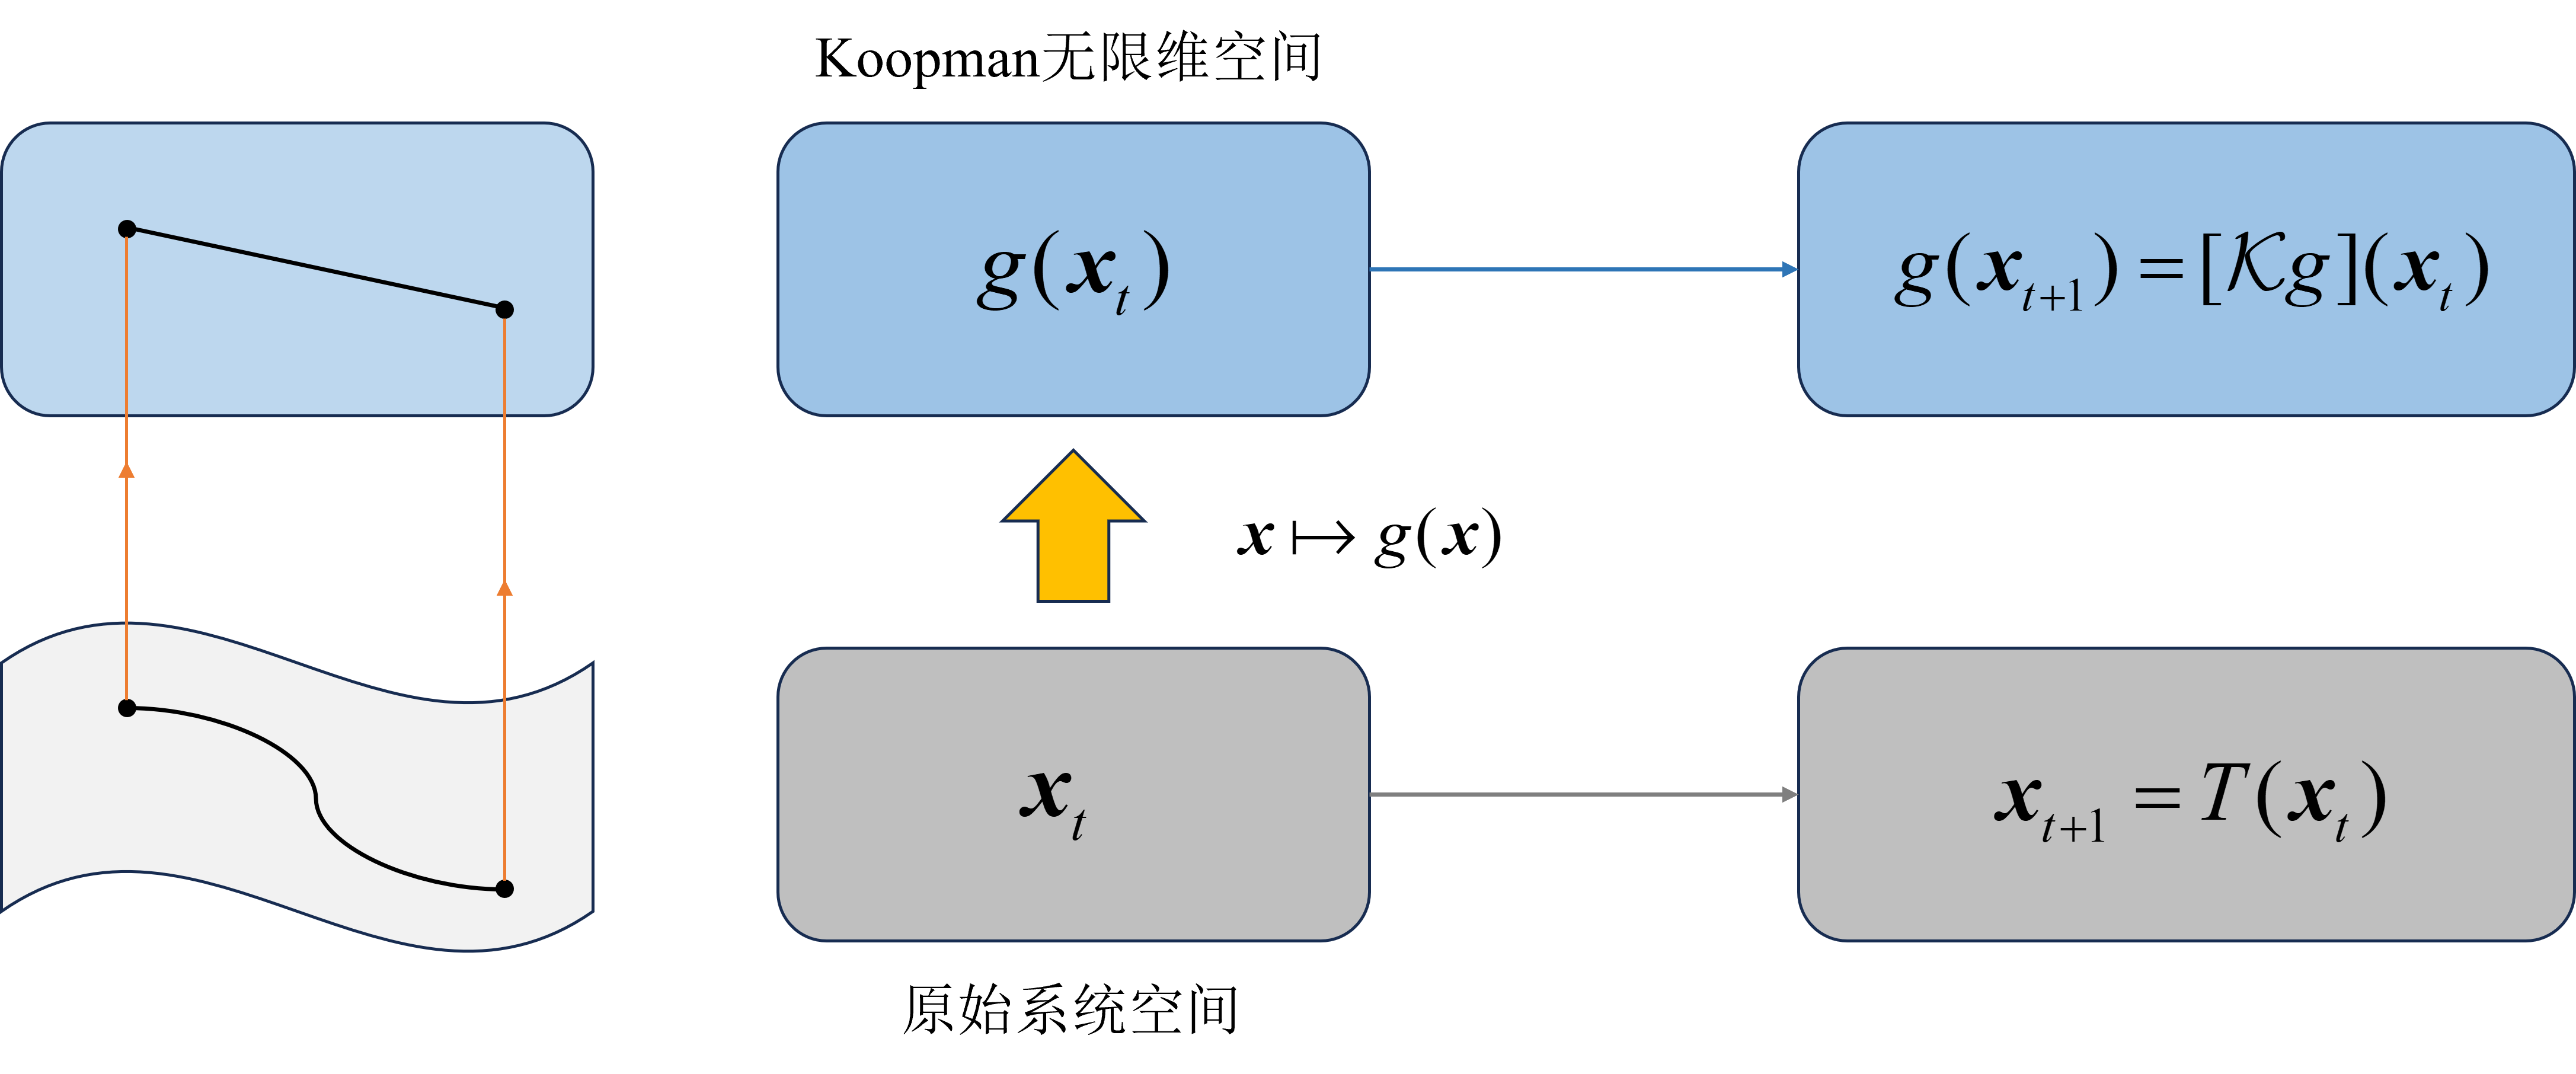
\includegraphics[width=32pc]{picture/3_1.png} 
	\caption{Koopman算子理论} \label{3_1}
\end{figure}
首先,考虑一个离散时间动力系统,其状态向量为$\bm{x} \in \mathcal{X} \subseteq \mathbb{R}^{N_{\bm{x}}}$,系统的演化由非线性函数$T$描述,如图 \ref{3_1} 所示。通过引入可观测函数$g(\bm{x})$,可以将原始状态 $\bm{x}$ 映射至新的空间。在该新空间中,系统动力学可通过线性算子 $\mathcal{K}$(即Koopman算子)来表述。换句话说,尽管 $T$ 和 $\mathcal{K}$ 作用于不同的空间,但它们封装了相同的动态特性。

例如,对于给定的当前状态 $\bm{x}$,可以通过两种方式将其推进到下一个时间步并进行观测:一是直接使用 $T$ 计算 $T(\bm{x})$,再对得到的状态进行观测(如图 \ref{3_1} 的下方路径所示);二是应用可观测函数 $g(\bm{x})$,随后作用于线性算子$\mathcal{K}$,并在 $\bm{x}$ 处进行评估(如图 \ref{3_1} 的上方路径所示)。这种“等价性”概念具有以下优势:

(1)使非线性动力系统 $T$ 在全局范围内以线性形式表示,从而可应用线性系统的分析与控制方法;

(2)通过实时学习线性算子来估计系统的底层动力学,避免对非线性函数进行最小二乘回归的需求,而后者通常需要大量数据。

% \subsection{基于Koopman理论的数据驱动预测}

% 考虑一个离散时间的动力学系统,其状态随着时间的推移演化,系统的状态在时间 \( t+1 \) 时刻由当前时刻 \( t \) 的状态决定,即:

% \begin{equation}
%     {\bm x}_{t+1} = T({\bm x}_t)
% \end{equation}

% 在这个框架下,考虑一个复值函数的向量空间 \( \mathcal{\bm F} \),其中包含了系统状态空间上的可观测量。可观测量 \( g \in \mathcal{\bm F} \) 可以看作是对系统状态的提升或映射。为了描述这些可观测量的演化,使用与系统动力学 \( T \) 相关联的Koopman算子 \( \mathcal{\bm K}: \mathcal{\bm F} \to \mathcal{\bm F} \),其作用是将可观测量 \( g \) 映射到时间 \( t+1 \) 时刻的状态上,即:

% \begin{equation}
%     \mathcal{\bm K} g = \bm g \circ T
% \end{equation}

% 这里,符号 \( \circ \) 表示函数的复合。为了确保Koopman算子的良定义,要求空间 \( \mathcal{F} \) 对 \( T \) 的复合是封闭的。也就是说,若 \(  g \in \mathcal{F} \),那么 \( \bm g \circ T \) 仍然属于 \( \mathcal{\bm F} \)。在某些情况下,如果 \( \mathcal{\bm F} \) 包含特定的预定义函数(如返回完整状态值的函数),这可能导致 \( \mathcal{\bm F} \) 变为无限维空间。根据Koopman算子的定义,它将系统的可观测量从时刻 \( t \) 推移到时刻 \( t+1 \):
% \begin{equation}
%     \mathcal{\bm K} g(\bm x_t) = g \circ T(\bm x_t) = g(T(\bm x_t)) = g(\bm x_{t+1})
% \end{equation}

% 通过这种方式,原本可能是非线性的系统在Koopman空间中变得线性化,从而使得可以使用线性系统理论来设计控制器。这一转换的关键在于可以通过提升状态 \( g(\bm x) \),将原系统转化为Koopman算子下的线性系统,进而在高维的空间中线性地描述系统的演化。

% 为了避免无限维空间的计算复杂性,通常选择在Koopman算子下具有不变性的有限维子空间 \( \mathcal{\bm S} \subset \mathcal{\bm F} \)。当限制Koopman算子的作用在这个有限维的子空间 \( \mathcal{\bm S} \) 上时,便可以得到一个有限维的矩阵表示,使得系统的演化可以用线性代数方法来进行处理:
% \begin{equation}
%     \mathcal{\bm K}\bm \Psi = \bm \Psi \circ T
% \end{equation}

% 其中,\( \bm \Psi \) 是有限维子空间 \( \mathcal{\bm S} \) 的基,表示该子空间中可观测量的集合。这样,系统的轨迹可以通过有限维矩阵的线性映射来描述,从而使得原本复杂的非线性系统变得可通过线性系统理论来分析和控制。

% 在实际应用中,通常通过采样系统的离散时间数据来估计Koopman算子的有限维近似。这一过程的核心是通过观察数据来构造一个有限维的Koopman算子矩阵,并且在该有限维空间内,系统的演化近似为一个线性系统。这种近似方法可以显著降低计算的复杂性,同时仍然能够有效地捕获系统的非线性特性。


% 对于具有控制输入的系统,Koopman理论同样适用,可以在控制系统中引入控制输入的影响,使得可以通过Koopman算子进行有效的建模和控制。

\section{模型预测控制方法}
本小节重点阐述模型预测控制(Model Predictive Control,MPC)的基本原理及其应用流程,结合鲁棒非线性控制方法和离散化建模,构建适用于无人机绳系吊运系统的完整控制设计框架。

MPC已被证明是一种高效的控制方法\cite{2003A},其核心思想包含三个关键要素:预测模型、滚动优化和反馈校正。
预测模型用于预测未来一段时间内的系统输出。其基本原理是根据历史信息 $\{ \bm u(k-j), \bm y(k-j) | j \geq 1 \}$ 以及未来输入 $\{ \bm u(k+j-1) | j = 1, \dots, m \}$来预测系统未来的响应 $\{ \bm y(k+j) | j = 1, \dots, p \}$。在实际应用中,递归优化方法通常作为在线优化策略,仅执行计算出的控制序列中的第一个控制值,随后在下一个采样时刻重新计算最优控制序列。
每次优化基于当前系统状态和预测模型进行,优化结果是一个控制输入序列,但实际执行时仅使用序列的第一个控制值,并在下一个时刻进行滚动更新。
反馈校正是MPC的重要组成部分,用于实时修正系统的输出误差。每个采样时刻,系统通过对比实际输出与预测输出之间的差异,对预测模型输出进行修正,并利用修正后的状态进行下一轮优化。
综上所述,MPC的整体工作原理如图 \ref{mpc} 所示。通过预测模型、滚动优化和反馈校正的有机结合,MPC能够在面对非线性系统、不确定性和外部扰动时,展现出优异的控制性能,实现对复杂系统的精确控制。

\begin{figure}[hbt!]
	\centering
	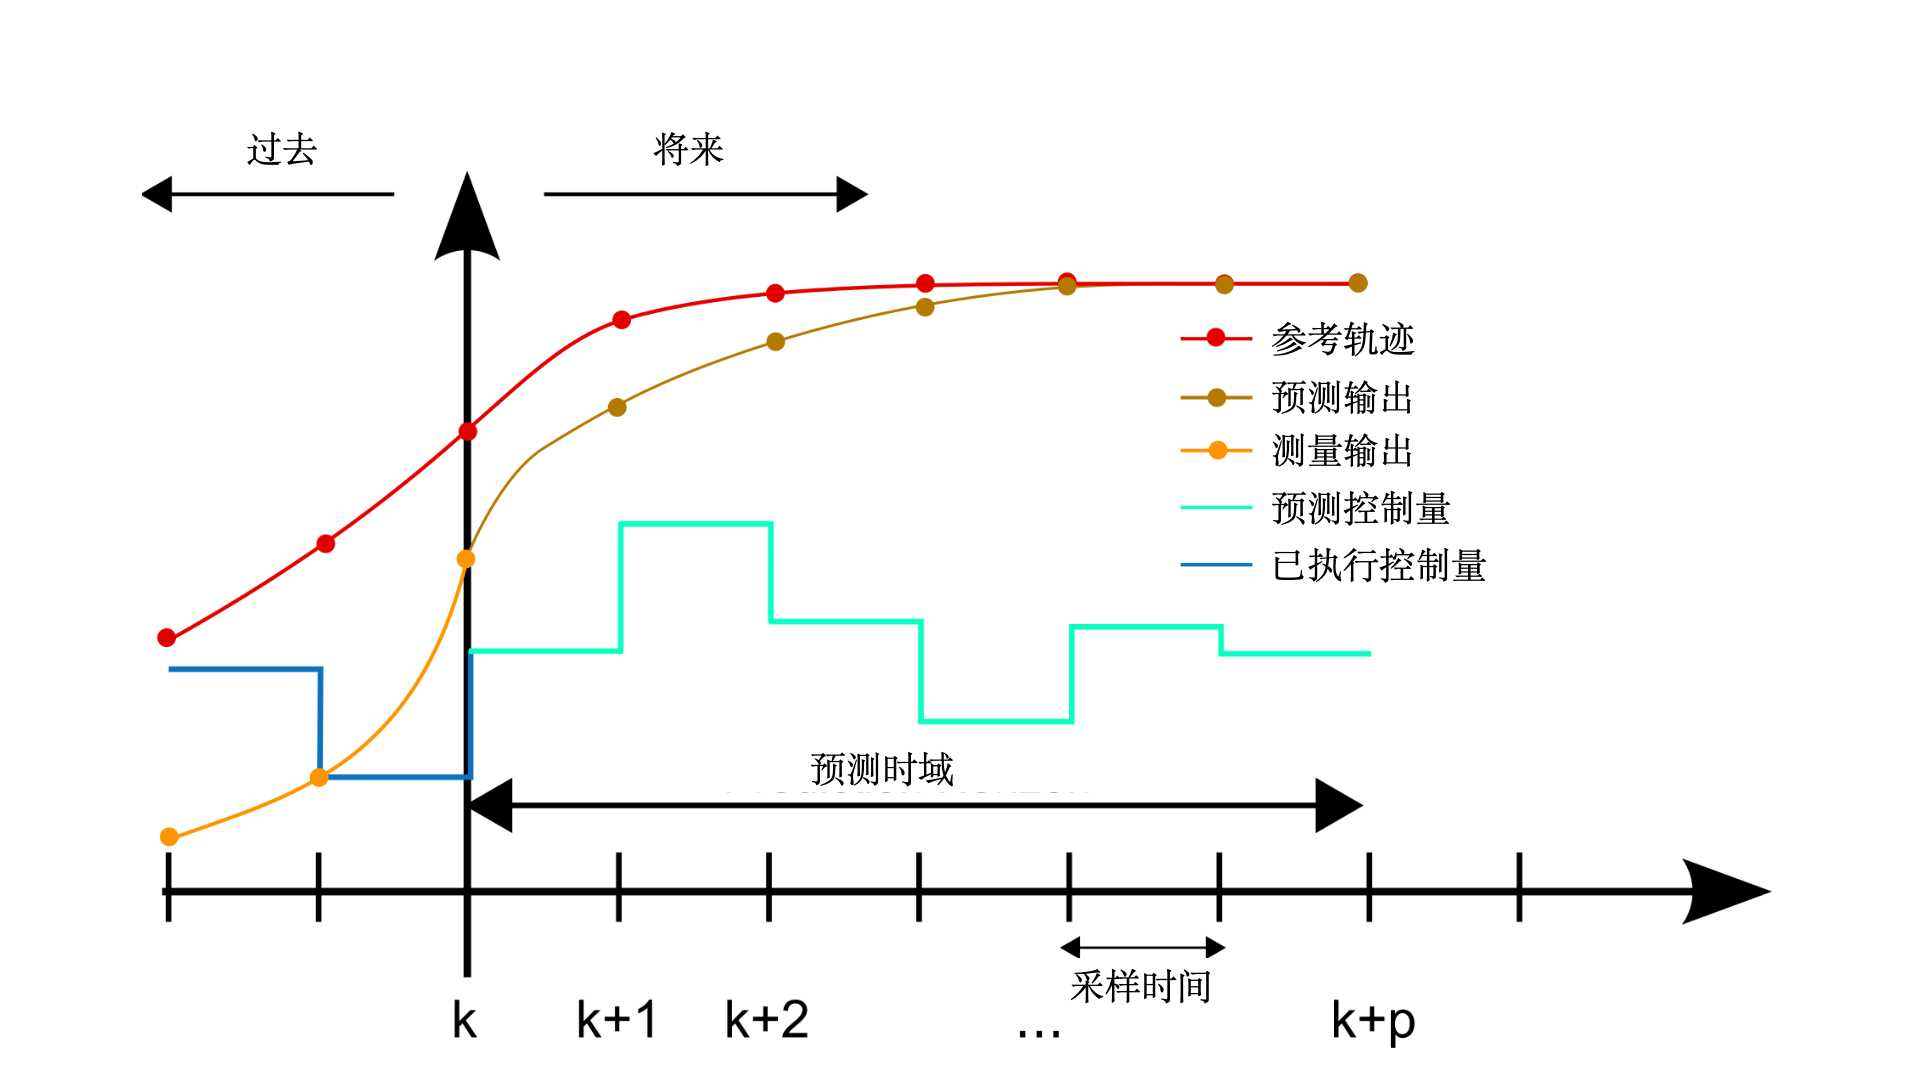
\includegraphics[width=40pc]{picture/mpc.jpg} 
	\caption{模型预测控制流程图} \label{mpc}
\end{figure}
MPC中的预测模型是基于状态空间模型构建的。通过测量或估计无人机的状态变量,预测未来时域内的系统状态参数,从而实现对系统的控制。其原理表达式如下:

\begin{equation}
	\begin{gathered}
\bm s(k+1) = \bm A(k)\bm s(k) + \bm B(k) \bm u(k)\\\bm O(k) = \bm C(k) \bm s(k)
\end{gathered}
\end{equation}
其中,$\bm s(k)$ 表示 $k$ 的系统状态,$\bm u(k)$ 表示 $k$ 时刻系统的控制输入,$\bm O(k)$ 为系统的输出。$\bm A(k)$ 是系统的状态转移矩阵,描述了当前时刻系统状态 $\bm s(k)  $对下一个时刻状态 $ \bm s(k+1)$ 的影响,
$\bm B(k)$  是控制输入矩阵,描述了系统的控制输入 $ \bm u(k)$ 对当前状态  $\bm s(k)$  及未来状态  $\bm s(k+1)$ 的影响,
$\bm C(k)$ 是输出矩阵,描述了系统的状态量 $\bm s(k)$ 如何转换为系统的观测输出 $\bm O(k)$。

通过建立预测模型,可以构造新的状态向量,该向量同时包含系统的状态变量与控制输入:

\begin{equation}
	\begin{gathered}\bm \xi(k)=\begin{bmatrix}\bm s(k)\\\bm u(k-1)\end{bmatrix}\\\bm \xi(k+1)=\begin{bmatrix}\bm s(k+1)\\\bm u(k)\end{bmatrix}=\begin{bmatrix}\bm A(k)\bm s(k)+\bm B(k)\bm u(k)\\\bm u(k-1)+\bm \Delta \bm u(k)\end{bmatrix}\end{gathered}
\end{equation}

由此,可以得到新的状态空间方程:

\begin{equation}
	\begin{aligned}\bm \xi(k+1)=\tilde{\bm A}&_k\bm \xi(k)+\tilde{\bm B}_k\bm \Delta \bm u(k)\\\bm O(k)&=\tilde{\bm C}_k\bm\xi(k)\end{aligned}
	\label{3-11}
\end{equation}
其中,$N_x$ 和 $N_u$ 分别表示状态变量和控制输入的维度,$E$ 为单位矩阵,
$$\bm{\tilde{A}}_k = \begin{bmatrix} \bm A(k) & \bm B(k) \\ \bm 0_{N_u \times N_x} & \bm E_{N_u} \end{bmatrix},$$
$$\tilde{\bm B}_k = \left[ \bm B(k) , \bm E_{N_u} \right]^\mathrm{T},$$
$$\tilde{\bm C}_k = \left[ \bm C(k) \quad \bm 0 \right]$$

根据状态预测模型,可以推导出未来时域内的系统状态:
\begin{equation}
    \bm \xi(k + N_c) = \tilde{\bm A}_k^{N_c} \bm \xi(k) + \tilde{\bm A}_k^{N_c-1} \tilde{\bm B}_k \bm \Delta \bm u(k) + \tilde{\bm A}_k^{N_c-2} \bm \tilde{\bm B}_k \bm \Delta \bm u(k+1) + \dots + \tilde{\bm B}_k \bm \Delta \bm u(k + N_c - 1)
\end{equation}
\begin{equation}
    \bm \xi(k + N_p) = \tilde{\bm A}_k^{N_p} \bm \xi(k) + \tilde{A}_k^{N_p-1} \tilde{\bm B}_k \bm \Delta \bm u(k) + \tilde{\bm A}_k^{N_p-2} \tilde{\bm B}_k \bm \Delta \bm u(k+1) + \dots + \tilde{\bm B}_k \bm \Delta \bm u(k + N_p - 1)
\end{equation}

通过上述推导,可以获得未来时刻的状态预测结果。基于新的状态空间方程\autoref{3-11},系统的输出量可进一步计算得到:
\begin{equation}
	\begin{aligned}
	\bm \sigma(k + N_c) =& \tilde{\bm C}_k \tilde{\bm A}_k^{N_c} \bm \xi(k) + \tilde{\bm C}_k \tilde{\bm A}_k^{N_c-1} \tilde{\bm B}_k \bm \Delta \bm u(k) +\\
	&\tilde{\bm C}_k \tilde{\bm A}_k^{N_c-2} \tilde{\bm B}_k \bm \Delta \bm u(k+1) + \dots + \tilde{\bm C}_k \tilde{\bm B}_k \bm \Delta \bm u(k + N_c - 1)
	\end{aligned}
\end{equation}
\begin{equation}
	\begin{aligned}
	\bm  \sigma(k + N_p) =& \tilde{\bm C}_k \tilde{\bm A}_k^{N_p}\bm  \xi(k) + \tilde{\bm C}_k \tilde{\bm A}_k^{N_p-1} \tilde{\bm B}_k \bm \Delta \bm u(k) +\\
	&\tilde{\bm C}_k \tilde{\bm A}_k^{N_p-2} \tilde{\bm B}_k \bm \Delta \bm u(k+1) + \dots + \tilde{\bm C}_k \tilde{\bm B}_k \bm  \Delta \bm u(k + N_p - 1)
	\end{aligned}
\end{equation}

综上,系统在未来时刻的输出可以用矩阵形式表示为:
\begin{equation}
    \bm O = \bm \Psi \bm \xi(k) + \bm \Theta \bm \Delta \bm U(k)
\end{equation}
其中$$
\boldsymbol{O} = 
\left[
	\boldsymbol{\sigma}(k+1) , \boldsymbol{\sigma}(k+2) , \boldsymbol{\sigma}(k+3) , \cdots , \boldsymbol{\sigma}(k+N_p)
\right]^\mathrm{T},$$
$$\boldsymbol{\Psi} = 
\left[
	\boldsymbol{\tilde{C}}_k\boldsymbol{\tilde{A}}_k , \boldsymbol{\tilde{C}}_k\boldsymbol{\tilde{A}}_k^2 , \boldsymbol{\tilde{C}}_k\boldsymbol{\tilde{A}}_k^3 , \cdots , \boldsymbol{\tilde{C}}_k\boldsymbol{\tilde{A}}_k^{N_p}
\right]^\mathrm{T},$$
$$\boldsymbol{\Delta U} = 
\left[
	\bm \Delta \bm u(k) , \bm \Delta \bm u(k+1) , \bm \Delta \bm u(k+2) , \cdots , \bm \Delta \bm u(k+N_c-1)
\right]^\mathrm{T},$$
$$\bm \Theta=\begin{bmatrix}\tilde{\bm C}_k\tilde{\bm B}_k&0&0&0\\\tilde{\bm C}_k\tilde{\bm A}_k\tilde{\bm B}_k&\tilde{\bm C}_k\tilde{\bm B}_k&0&0\\...&\ddots&...&...\\\tilde{\bm C}_k\tilde{\bm A}_k^{N_c-1}\tilde{\bm B}_k&\tilde{\bm C}_k\tilde{\bm A}_k^{N_c-2}\tilde{\bm B}_k&...&\tilde{\bm C}_k\tilde{\bm B}_k\\...&...&...&...\\...&...&...&...\\\tilde{\bm C}_k\tilde{\bm A}_k^{N_p-1}\tilde{\bm B}_k&\tilde{\bm C}_k\tilde{\bm A}_k^{N_p-2}\tilde{\bm B}_k&...&\tilde{\bm C}_k\tilde{\bm A}_k^{N_p-N_c-1}\tilde{\bm B}_k\end{bmatrix}$$

针对不同的控制问题,可以根据该方法的理论框架设计相应的代价函数和约束条件,并采用合适的优化方法进行求解,从而得到符合约束条件的最优控制量序列。本文将模型预测控制理论应用于无人机控制器的设计,并利用二次规划方法(QP)进行求解。

\section{基于数据驱动的混合模型设计}
本节将详细介绍所提出的Neural Predictor框架的原理和实现方法。该方法的核心思想是将外力$\bm{f}_e$和力矩$\bm{\tau}_e$建模为动态系统,并通过基于Koopman算子的数据驱动的方法对其进行学习。具体来说,该框架利用由Koopman算子理论导出的升维线性系统(Lifted Linear System, LLS),以显式的方式捕捉外力和力矩的动态特性。
\subsection{数据驱动模型构建方法}
Koopman算子可以从数据中将非线性系统全局映射为线性系统 \cite{Mamakoukas2023}。这一性质为以数据驱动的方式显式捕捉未知非线性动力学(如式 (\ref{3-1}) 中的$\bm f_e$和$\bm \tau_e$)提供了途径。因此,本文采用这一方法,通过数据驱动的方式学习$\bm{f}_e$和$\bm{\tau}_e$。升维线性系统的基本概念简述如下:

考虑一个具有控制输入的未知非线性动力学系统: 
\begin{equation} 
	\dot{\bm{x}} = {f}(\bm{x},\bm{u}) \label{nonlinear_input} \end{equation} 
其中$\bm{x} \in \mathbb{R}^n$为系统状态,$\bm{u} \in \mathbb{R}^p$为控制输入。定义一组标量值函数${g}$作为升维函数,该函数集构成了一个无限维的Hilbert空间$\mathcal{\bm H}$。假设这些升维函数可以表示为: 
\begin{equation} 
	{g}(\bm{x},\bm{u}) = {\Psi}(\bm{x}) + \bm{L}\bm{u} 
\end{equation} 
其中$\bm{L}$为常数矩阵。在假设控制输入$\bm{u}$ 不会在Hilbert空间 $\mathcal{H}$ 中演化的条件下,式(\ref{nonlinear_input})中的非线性动力学系统可以重新表述为: 
\begin{equation} 
	{\Psi}(\bm{x}(t_0+t_s)) = {\mathcal{K}} {g}(\bm{x}(t_0), \bm{u}(t_0)) = \begin{bmatrix}\bm A&\bm B\end{bmatrix}\begin{bmatrix}\Psi(\bm x)\\\bm u\end{bmatrix}
\label{3-21} 
\end{equation} 
其中,$\bm{x}(t_0+t_s)=\bm{x}(t_0)+\int_{t_0}^{t_0+t_s}{f}(\bm{x},\bm{u}){\mathrm{d}t}$,$t_s$ 为采样时间$t_s$。上述公式描述了升维函数${g}(\bm{x},\bm{u})$的前向时间演化。令$\bm{z}(t) \triangleq {\Psi}(\bm{x}(t))$,可以将式(\ref{3-21})改写为: 
\begin{equation} \bm{z}(t_0 + t_s) = \bm{A}\bm{z}(t_0) + \bm{B}\bm{u}(t_0) \label{lls} 
\end{equation} 
这就是未知非线性动力学系统(\ref{nonlinear_input})的升维线性系统。

如果给定非线性系统(\ref{nonlinear_input})的一组数据序列 $\{(\bm{x}_1,\bm{u}_1),\cdots,(\bm{x}_{T-1},\bm{u}_{T-1}),(\bm{x}_T)\}$,则可以通过求解以下最小二乘优化问题来近似估计矩阵$\bm{A}$和$\bm{B}$:
\begin{equation}
	\bm{A},\bm{B} = \mathop{\arg\min\limits_{\bm{A},\bm{B}}} \Vert \bm{Z}_{2:T} - (\bm{A}\bm{Z}_{1:T-1}+\bm{B}\bm{U}_{1:T-1}) \Vert \label{LS_AB}
\end{equation} 
其中,$\bm{Z}_{1:T-1}= [ \bm{z}_1,\bm{z}_2,\cdots,\bm{z}_{T-1} ]^\mathrm{T}$,$\bm{Z}_{2:T}= [\bm{z}_2,\bm{z}_3,\cdots,\bm{z}_{T}]^\mathrm{T}$,$\bm{U}_{1:T-1}= [\bm{u}_1,\bm{u}_2,\cdots,\bm{u}_{T-1}]^\mathrm{T}$,$\bm{z}_i$ 表示对应于第 $i$ 个样本 $\bm{x}_i\ (i=1,2,\cdots,T)$ 的状态。当$\bm{Z}_{1:T-1}$和$\bm{U}_{1:T-1}$的序列长度$T$有限时,上述优化问题实际上对Koopman算子进行了有限维近似 \cite{Hao2024}。

式(\ref{lls})是以数据驱动的方式推导得到的离散形式。因此,根据式 (\ref{lls}),未知非线性系统(\ref{nonlinear_input})的连续有限维近似形式可以表示为:
\begin{equation}
	\begin{gathered}\dot{\boldsymbol{z}}=\boldsymbol{A}_{c}\boldsymbol{z}+\boldsymbol{B}_{c}\boldsymbol{u}\\\boldsymbol{x}=\boldsymbol{C}\boldsymbol{z}\end{gathered}
	\label{lift_linear}
\end{equation}
其中$\bm{A_c}=\log(\bm{A})/t_s$, $\bm{B_c}=\bm{B}/(\int_{0}^{t_s}e^{\bm{A}t}\text{dt})$, $\bm{z} = {\Psi}(\bm{x}):\mathbb{R}^n \rightarrow \mathbb{R}^K$, $K\gg n$, $\bm{u}\in \mathbb{R}^p$, $\bm{A_c} \in \mathbb{R}^{K\times K}$,  $\bm{B_c} \in \mathbb{R}^{K\times p}$, $\bm{C} \in \mathbb{R}^{n\times K}$,$t_s$为采样时间间隔。

\subsection{数据驱动方法建模未知外力和力矩}
在无人机绳系吊运系统中,系绳对无人机施加的外力 $\bm{f}_e$ 和力矩 $\bm{\tau}_e$ 体现了无人机的未知动态特性。假设外力和力矩的未知动力学系统可表示为以下形式:
\begin{equation}
	\dot{\bm \chi} = {\xi}(\bm \chi,\bm \zeta) \label{dynamics}
\end{equation}
其中 $\bm \chi = [f_e, \bm \tau_e]^\mathrm{T}$,${\xi}$ 表示外力和力矩的未知动力学,$\bm{\zeta}$ 表示系统的控制输入,通常由无人机的状态或部分子状态构成。本文中,$\bm{\zeta}$ 选取无人机的线速度与角速度作为控制输入。

如上所述,式 (\ref{dynamics}) 中的未知非线性动力学可以通过有限维的升维线性系统(\autoref{lift_linear})从数据中捕捉。然而,捕捉的关键在于如何寻找合适的升维函数 ${\Psi}$。为此,本文提出了一种由权重 $\bm{\theta} = {W^1, \cdots, W^{L+1}}$ 参数化的深度神经网络,用于近似有限维升维函数,其表达式如下:
\begin{equation}
	{\Psi}(\bm \chi;\bm{\theta}) = W^{L+1}\phi(W^L(\cdots \phi(W^1 \bm \chi \cdots)) \label{dnn}
\end{equation}
其中,$\phi$ 是ReLU激活函数。由于深度神经网络具有卓越的函数拟合和逼近能力,因此采用它来近似升维函数,为了确定与 Koopman 算子相关联的升维函数,通过最小化以下损失函数进行训练:
\begin{equation}
	L = \beta_1 L_{\text{recons}} + \beta_2 L_{\text{forward}} + \beta_3 L_{\text{backward}}
\end{equation}
其中 $\beta_1$、$\beta_2$ 和 $\beta_3$ 是正的超参数,分别衡量三种损失函数的权重。三个损失函数 $L_{\text{recons}}$、$L_{\text{forward}}$ 和 $L_{\text{backward}}$ 的定义如下:

(1)状态重建损失函数 $L_{\text{recons}}$:非线性系统的状态应当从不变的Hilbert空间 $\mathcal{H}$ 中重建。重建损失函数 $L_{\text{recons}}$ 定义如下以使得重建误差尽可能地小:
\begin{equation}
	L_{\text{recons}}=\Vert \bm{f}_e(t) - \bm{C} \bm{z}(t) \Vert
\end{equation}

(2)多步预测损失函数 $L_{\text{forward}}$ 和 $L_{\text{backward}}$: 从带有基准控制器的无人机系绳吊运系统中采样数据,构建包含 $s$ 条轨迹的数据集 $\{\bm{X}_i \in \mathbb{R}^{n\times m}, \bm{U}_i \in \mathbb{R}^{p \times m}, i=1,\cdots,s\}$。数据集中的每条轨迹都含有 $m$ 个时间步长的数据。每个采样时刻的训练标签,即外力 $\bm{f}_e$ 和力矩 $\bm{\tau}_e$,由四旋翼动力学方程 (\ref{3-1}) 计算得到。

每个采样时刻的状态可以表示为 $\bm{Z}_i = [\bm{z}_0^i,\cdots,\bm{z}_{m-1}^i]=[{\Psi}(\bm{\chi_{0}}^i),\cdots,{\Psi}(\bm{\chi}_{m-1}^i)]\in \mathbb{R}^{K\times m}$。
通过迭代升维线性系统(\ref{lift_linear}),基于初始状态 $\bm{z}_0^i$ 来预测前向和后向状态,分别表示为$\hat{\bm{Z}}_i^{\text{forward}} = [\hat{\bm{z}}_0^i, \cdots, \hat{\bm{z}}_{m-1}^i]$ 和 $\hat{\bm{Z}}_i^{\text{backward}} = [\hat{\bm{z}}_0^i, \cdots, \hat{\bm{z}}_{m-1}^i]$。

定义如下损失函数来使得升维线性系统的前向和后向预测误差尽可能地小:
\begin{equation}
	\begin{aligned}
		L_{\text{forward}} = \sum_{i=1}^{k} \mu_1^{i} {\rm MSE}(\bm{Z_{i}},\hat{\bm{Z_{i}}}^{\text{forward}})  \\
		L_{\text{backward}} = \sum_{i=1}^{k} \mu_2^{i} {\rm MSE}(\bm{Z_{i}},\hat{\bm{Z_{i}}}^{\text{backward}})\label{L2}
	\end{aligned}
\end{equation}
其中 $\mu_1,\mu_2 \in(\text{0},\text{1})$ 为超参数,用于调整损失项的时间步长权重。损失函数(\ref{L2})的目的是最小化前向和后向多步预测误差,从而有助于在较长的预测时间范围内更精确地预测系统状态。

\subsection{数据驱动建模方法收敛性证明}
尽管学习得到的模型能够较好地拟合外力与力矩的动态特性,但其预测结果可能存在发散的风险,从而导致外力和力矩的预测不准确。为了确保学习过程中的预测误差在全局范围内保持可控,需要对预测误差进行约束。以下定理为学习得到的模型的预测误差提供了全局有界性的理论保证。

\textbf{定理3.1:}假设存在正数 $\alpha_{\bm{\chi}}>0$ 和 $\alpha_{\bm{\zeta}}>0$,使得不等式 $\Vert \bm{\chi}(t_0+t_s)-\bm{\chi}(t_0)\Vert \le \alpha_{\bm{\chi}}$ 和 $\Vert \bm{\zeta}(t_0+t_s) - \bm{\zeta}(t_0) \Vert \le \alpha_{\bm{\zeta}}$ 成立,如果近似得到的Koopman算子 $\hat{{\mathcal{K}}}$ 是稳定的,且与其相关的升维函数具有Lipschitz常数 $L_{\bm{\Psi}}$,则学习得到的模型的预测误差是全局有界的。

\textbf{证明:}
在时刻 \( t_0 + n\Delta t \),定义升维函数在真实状态 \( s(t_0 + n\Delta t) \) 下的值为 
$
\Psi(s(t_0 + n\Delta t))$,
其近似解为$
\tilde{\Psi}_n
$,
其中 $ n \in \mathbb{Z}^+ $ 表示向前推进的时间步数。

局部误差描述模型在单个时间步长内的精度,而全局误差描述模型在所有时间步长内的累积精度。用$e_n$表示由近似的 Koopman 算子 \( \tilde{\mathcal{K}}_d \)引起的第 \( n \)个时间步的局部误差,假设 Koopman 算子从前一个时间步开始传播升维函数的真实值,即:
\begin{equation}
	e_n\equiv\Psi(s(t_0+n\Delta t))-\tilde{\mathcal{K}}_d\Psi(s(t_0+(n-1)\Delta t))
	\label{k}
\end{equation}

该假设意味着 Koopman 算子可以传播上一时间步的升维函数真实值。此外,第 \( n \) 个时间步的全局误差记为 $E_n$,表示 Koopman 算子从初始时刻传播升维函数的真实值。类似地,第\( n \) 个时间步的全局误差$E_n$定义为:
\begin{equation}
	E_n\equiv\Psi(s(t_0+n\Delta t))-\tilde{\mathcal{K}}_d^n\Psi(s(t_0))
	\label{kk}
\end{equation}

当 \( n = 1 \) 时,全局误差与局部误差相等。然而,需要注意的是,全局误差(式(\ref{kk}))并不是局部误差(式(\ref{k}))的累积:,即
$
E_n \neq \sum_{i=1}^n e_i
$。
\autoref{3_2}中显示了局部误差与全局误差之间的区别。

令$z(x)=\Psi(s(x))$,基于近似Koopman算子 $\hat{{\mathcal{K}}}$ 的预测误差在经历 $n$ 个采样时刻后的全局误差表示为:
\begin{equation}
	{E}_n = {z}(t_0 + nt_s) - \tilde{\mathcal{K}}_d^n {z}(t_0)
\end{equation}
	
通过对\autoref{lls}进行递归迭代, 全局预测误差可以表示为:
\begin{equation}
	\begin{aligned}
	\Vert {E_n} \Vert &= \Vert {\Psi}(t_0+nt_s) -\tilde{\mathcal{K}}_d^n {\Psi}(t_0) \Vert  \\
	&=\Vert \sum_{i=0}^{n-1}\tilde{\mathcal{K}}_d^i\bm{e}(t_0+(n-i)t_s)\Vert \\
	&\le \sum_{i=0}^{n-1}\Vert \tilde{\mathcal{K}}_d^i\Vert \cdot \Vert \bm{e}(t_0+(n-i)t_s) \Vert
\end{aligned}
\end{equation}
其中,局部预测误差 $\bm{e}(t)=\bm{\hat{\chi}}(t)-\bm{\chi}(t)$,$\bm{\hat{\chi}}$ 表示对外力和力矩的预测值。

由于 $\bm{\chi}$, $\bm{\zeta}$ 和升维函数 ${\Psi}$ 是Lipschitz连续的,根据文献\oldcite{Hao2024}中的定理1,局部预测误差 $\bm{e}(t)$ 有界,即:
\begin{equation}
	\begin{aligned}
	\lim_{n_h\rightarrow \infty} \text{sup} \Vert \bm{e}(t) \Vert &=(\Vert \bm{CA} \Vert L_{\bm{\Psi}}+1) \alpha_{\bm{\chi}}+\Vert \bm{CB}\Vert \alpha_{\bm{\zeta}} +\max_{\overline{\bm{\chi}}\in \mathbb{B}} \Vert \overline{\bm{\chi}} -\bm{C} \Psi\bm{(\overline{\bm{\chi}}}) \Vert \triangleq c
\end{aligned}
\end{equation}
其中,$n_h$ 是升维函数中最后一个隐藏层的层数,$\mathbb{B}$ 是包含每个采样时刻 $\bm{\chi}$ 的集合。由于局部预测误差 $\bm{e}(t)$ 有界,且近似Koopman算子 $\hat{\bm{\mathcal{K}}}$ 稳定,可以得到:
\begin{equation}
	\Vert \bm{E_n} \Vert \le \sum_{i=0}^{n-1}\Vert \tilde{\mathcal{K}}_d^i\Vert \cdot \Vert \bm{e}(t_0+(n-i)t_s) \Vert\le \Vert c \Vert \sum_{i=0}^{n-1}\Vert {\mathcal{K}}_d^i \Vert
\end{equation}
即预测误差是有界的,从而证明了学习模型的全局误差在理论上是有界的,进一步确保了模型的稳定性和预测的准确性。

\begin{figure}[hbt!]
	\centering
	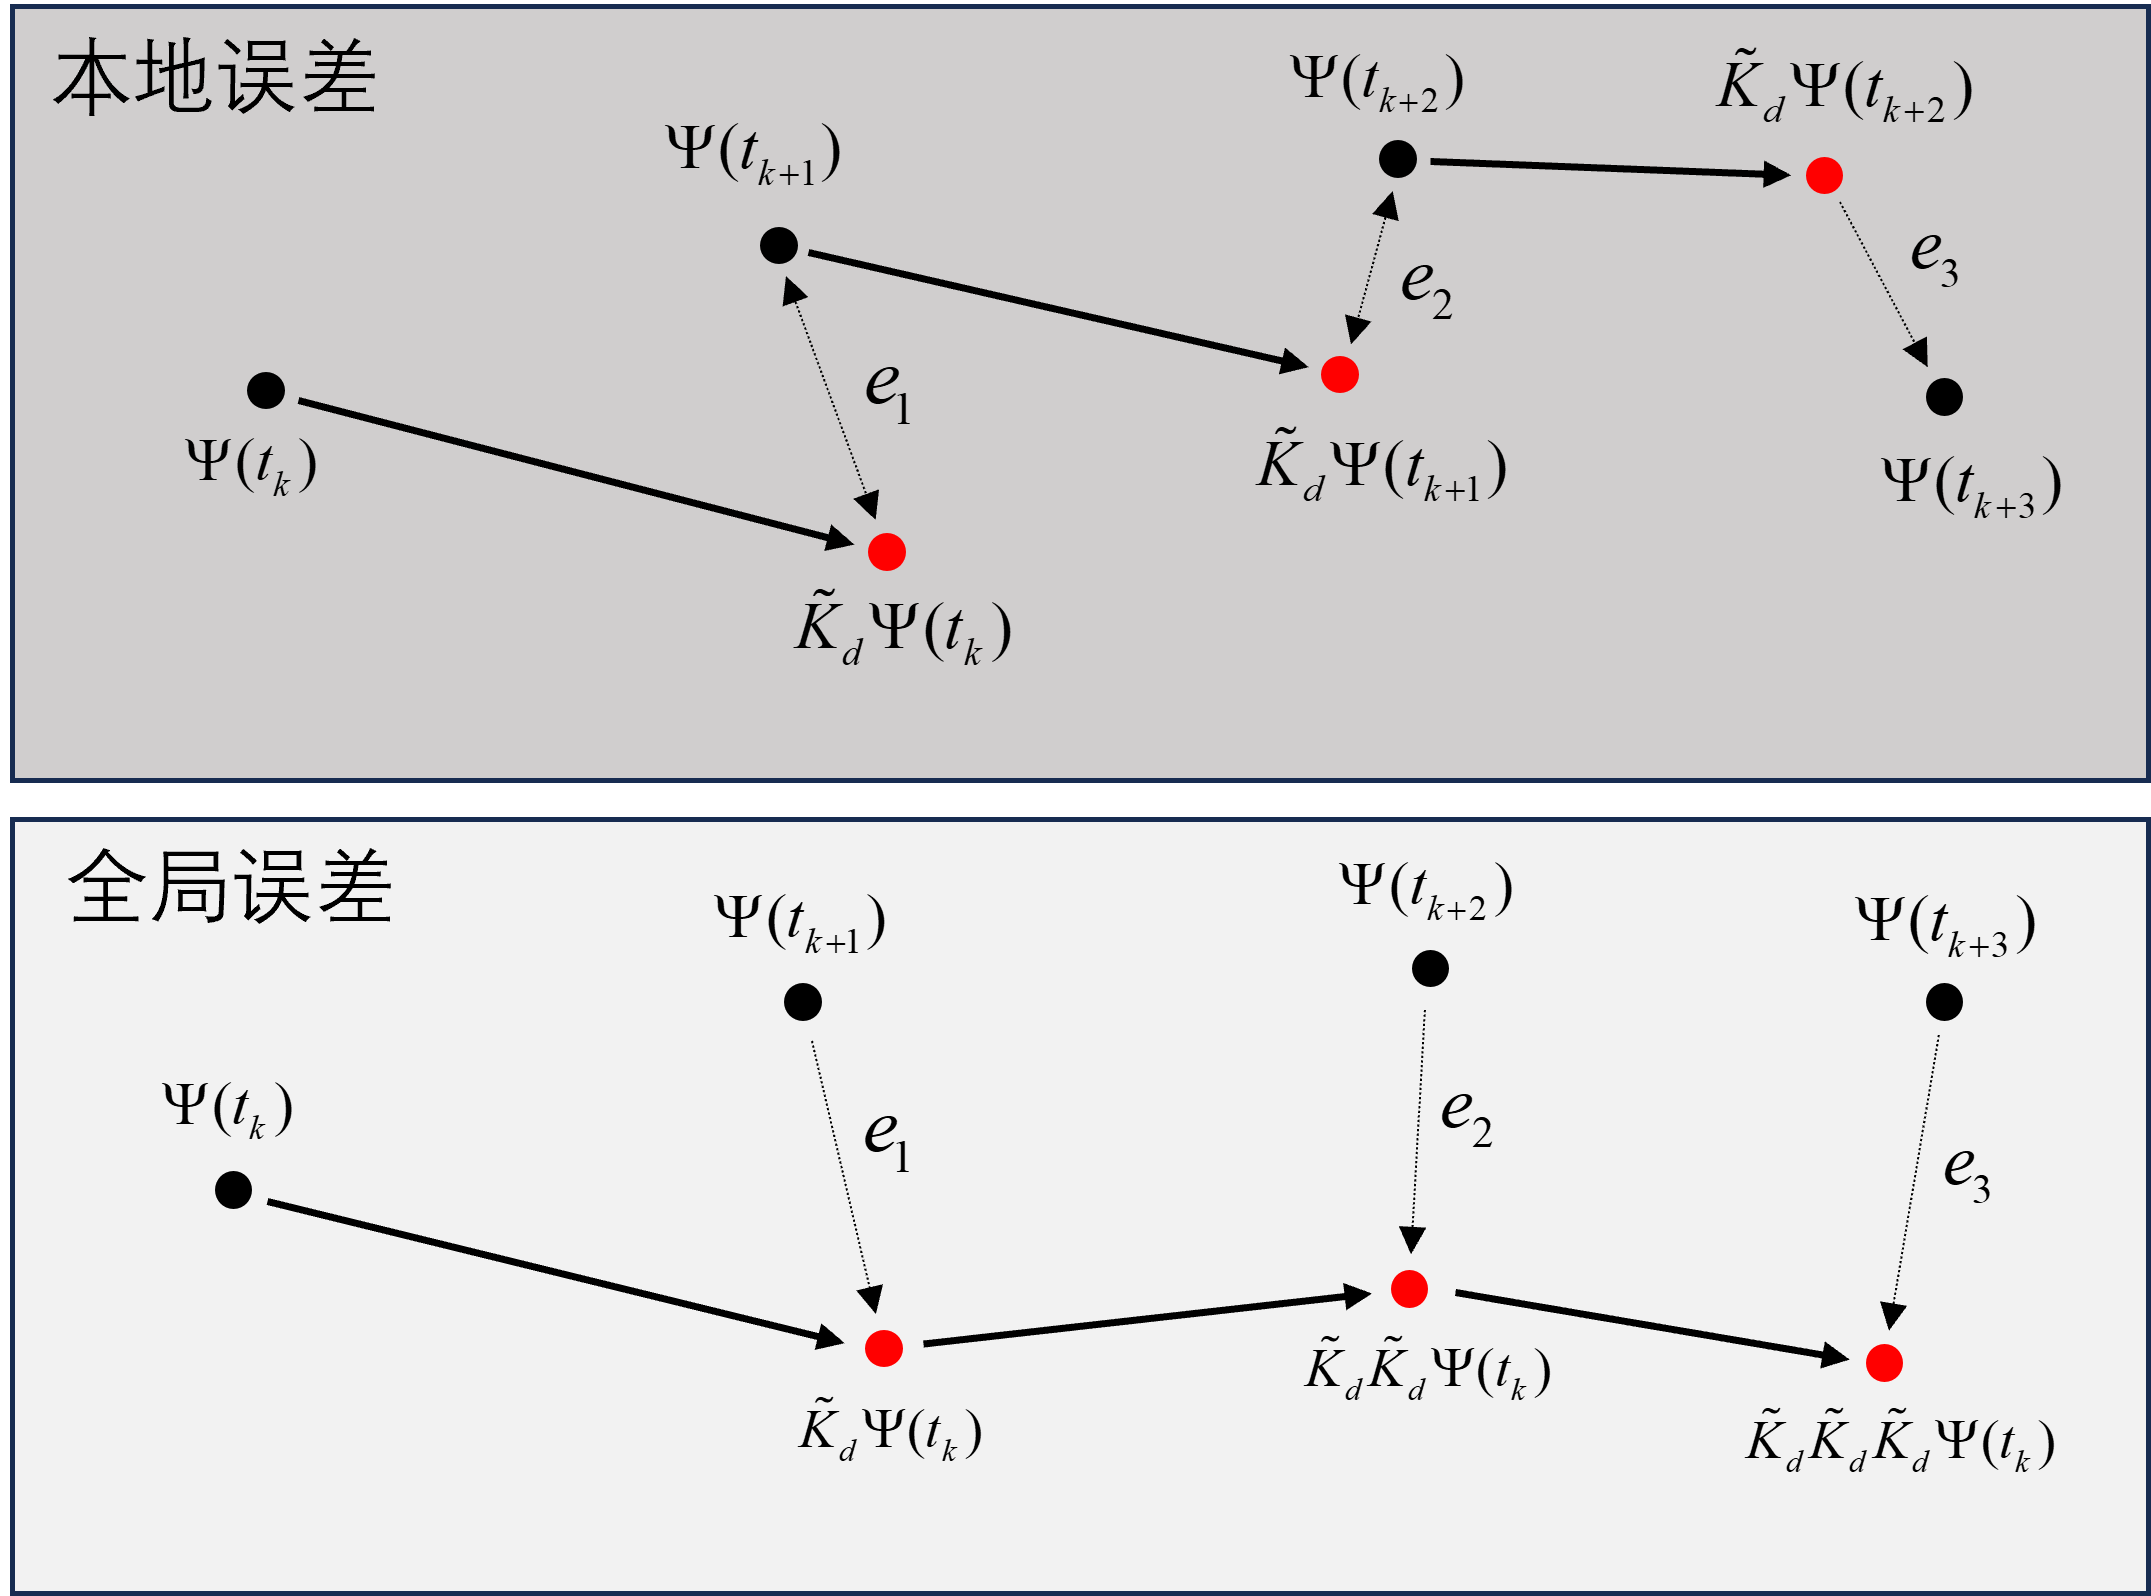
\includegraphics[width=28pc]{picture/3_2.png} 
	\caption{近似Koopman算子引起的局部误差和全局误差} \label{3_2}
\end{figure}
% 综上所述,上述定理表明,在满足特定条件下,学习到的动力学模型的预测误差在全局范围内是有界的,这确保了模型的稳定性和预测的准确性。
如\textbf{定理 3.1} 所述,当升维函数 $\Psi$ 具有Lipschitz常数时,预测误差是有界的。为了实现这一目标,采用谱归一化(Spectral Normalization, SN)方法约束升维函数 ${\Psi}$ 的Lipschitz常数。

根据定义,函数 $\rho$ 的Lipschitz常数等于其梯度的最大谱范数,即 $\Vert \rho \Vert_{\text{Lip}} = \sup \sigma (\nabla \rho)$。因此,对于由式(\ref{dnn})参数化的升维函数 ${\Psi}$,可以通过约束每一层的谱范数来限制其Lipschitz常数。

线性层 $g(\bm{x})=\bm{W}\bm{x}$ 的Lipschitz常数为 $\Vert g \Vert_{\text{Lip}} = \sup \sigma(\nabla(g))=\sup \sigma(\bm{W})=\sigma(\bm{W})$。因此,升维函数${\Psi}$的Lipschitz常数可以计算为:
% ($\Vert g_1 \circ g_2 \Vert_{\text{Lip}} \le \Vert g_1 \Vert_{\text{Lip}}\cdot \Vert g_2 \Vert_{\text{Lip}}$):
\begin{equation}
    \begin{aligned}
	\Vert {\Psi}(\bm{\chi}) \Vert_{\text{Lip}} &\le \Vert g^{L+1} \Vert_{\text{Lip}} \cdot \Vert \phi_L \Vert_{\text{Lip}} \cdots \Vert \phi_1 \Vert_{\text{Lip}} \cdot \Vert g_1 \Vert_{\text{Lip}} \\
	&= \prod_{l=1}^{L+1}\sigma(\bm{W}^l)
\end{aligned}
\end{equation}
其中,ReLU激活函数的Lipschitz常数为1,即 $\Vert \phi_l \Vert_{\text{Lip}} = 1$。在训练过程中,对每一层的权重 $\bm{W}$ 进行谱归一化,可以表示为:
\begin{equation}
    \hat{\bm{W}} = \bm{W} / \sigma(\bm{W}) \cdot \gamma ^{\frac{1}{L+1}}  
	\label{sn}
\end{equation}
其中,$\gamma$ 表示对整体 Lipschitz 常数的约束,$L$ 为神经网络的层数,$\sigma(\bm{W})$ 表示矩阵 $\bm{W}$ 的最大奇异值。

\textbf{引理3.1:}通过对升维函数应用谱归一化方法(\ref{sn})之后,升维函数的Lipschitz常数将满足以下约束:
\begin{equation}
	\Vert {\Psi}(\bm{\chi}) \Vert_{\text{Lip}}\le \gamma
\end{equation}
其中,$\gamma$ 是升维函数的目标Lipschitz常数。

\textbf{证明:}对DNN的每一层应用谱归一化方法,升维函数的Lipschitz常数满足:
\begin{equation}
	\Vert {\Psi}(\bm{\chi}) \Vert_{\text{Lip}} \le \prod_{l=1}^{L+1}\sigma(\hat{\bm{W}}^l) = \prod_{l=1}^{L+1}\gamma^{\frac{1}{L+1}}=\gamma
\end{equation}

因此,通过谱归一化方法可以有效限制升维函数的Lipschitz常数。\autoref{sn} 确保了升维函数 $\Psi$ 的 Lipschitz 常数受控,从而保证模型的稳定性和预测误差的有界性。

% 综上所述,在深度神经网络的训练过程中,谱归一化是一种有效的正则化策略,引入谱归一化技术不仅能够确保网络的Lipschitz常数满足特定的约束,还能提高模型的稳定性和泛化能力。这种方法在实现对升维函数约束的同时,避免了直接优化Lipschitz常数所带来的计算复杂性,从而为动态系统的学习提供了更加稳健的理论支撑。
% 通过对升维函数应用谱归一化方法,可以有效地控制其Lipschitz常数,从而保证模型的稳定性,并确保预测误差的有界性。这一方法不仅提供了对神经网络训练过程中的梯度传播的控制,也为避免过度拟合和梯度爆炸等问题提供了一种有效的解决方案。

\section{基于混合模型的模型预测控制器设计}
传统的鲁棒模型预测控制方法虽然能够有效应对系统中的不确定性,但其实际应用往往受到严格假设条件的限制,难以完全满足实际工程需求。此外,模型预测控制的闭环性能在很大程度上依赖于其内部模型的准确性,模型误差可能导致控制效果的下降。

为了解决上述问题,本小节引入了前文所提出的数据驱动建模方法Neural Predictor。该方法凭借其强大的数据拟合能力,能够捕捉系统中难以建模或存在动态缺失的特性,从而显著提升控制器的整体性能和鲁棒性。该算法的流程图如\autoref{illustration_framework} 所示。

\begin{figure}[hbt!]
	\centering
	\includegraphics[width=38pc]{picture/3_3.png} 
	\caption{数据驱动下的模型预测控制框架} 
	\label{illustration_framework}
\end{figure}
将 Neural Predictor 集成至 MPC 框架中,形成了针对无人机系绳吊运系统的数据驱动模型预测控制框架——NP-MPC。MPC 通过递推优化方法生成一系列最优控制输入。因此,NP-MPC可以被考虑在如下形式的优化问题中:
\begin{equation}
	\begin{aligned} \label{nmpc}
		&\operatorname*{minimize}_{\bm{\bar{u}}}& & \sum_{i=0}^{N-1}\left(\bm{\bar{x}}_i^\mathrm{T}\bm{Q}\bm{\bar{x}}_i + \bm{\bar{u}}_i^\mathrm{T}\bm{R}\bm{\bar{u}}_i\right) + \bm{\bar{x}}_N^\mathrm{T}\bm{P}\bm{\bar{x}}_N  \\
		&\text{subject to}& & \begin{aligned}
			&\bm{\bar{x}}_{0} = \bm{x}_k, \quad \bm{\bar{x}}_{N} \in \mathcal{X}_f, \\
			&\bm{\bar{x}}_{i+1} = {f}_{\text{nominal}}(\bm{\bar{x}}_i, \bm{\bar{u}}_i) + {f}_{\text{learned}},
		\end{aligned} \\
		&&& \bm{\bar{x}}_i \in \mathcal{X}, \quad \bm{\bar{u}}_i \in \mathcal{U}, \quad \forall i = 0, \ldots, N-1
	\end{aligned}
\end{equation}
其中,$\bm{x}_k$表示无人机在时间$k$时刻的状态,$\bm{\bar{x}}_i$和$\bm{\bar{u}}_i$分别是时间$k$的预测状态和控制输入,$N$是预测时域长度,$\mathcal{X}$、$\mathcal{U}$和$\mathcal{X}_f$分别是状态、控制输入和终端状态的约束集,$\bm{Q}$和$\bm{R}$是状态和控制输入的权重矩阵,$\bm{P}$是终端状态的权重矩阵。${f}_{\text{nominal}}$是无人机的名义模型,而${f}_{\text{learned}}$是通过升维线性系统学习得到的动态特性。

该优化问题采用序列二次规划(SQP)进行求解,并在实时迭代(RTI)方案中利用高斯-牛顿海森近似(Gauss-Newton Hessian Approximation)以提升计算效率。该方法将学习得到的动态特性融合到传统的名义模型中,从而提升控制器的性能和鲁棒性,有效地提升无人机在复杂环境中的自主飞行能力和轨迹跟踪精度。

\section{仿真验证}
在本节中,通过数值仿真验证了 Neural Predictor   (NP) 的性能,并在闭环控制中验证了NP-MPC的效果,旨在证明所提出方案的有效性。升维函数 $\Psi$ 由一个两层的深度神经网络参数化,每层包含128个神经元,深度神经网络的激活函数选用ReLU函数,线性升维系统的维度 $K$ 被设定为24。

在外力和力矩估计方面,将Neural Predictor与当前最先进的基于学习的估计方法NeuroMHE \cite{Wang2024e} 和 NeuroBEM \cite{Bauersfeld2021} 进行了对比,以展示Neural Predictor方法在捕捉外力和力矩方面的优势。训练和验证所用数据集与文献 \oldcite{Bauersfeld2021} 中提出的 dataset3 相同。Neural Predictor与NeuroMHE一样采用监督学习进行训练,输入为无人机的线速度和角速度。为确保公平比较,训练数据集选取了一个时长为 10 秒的“摇摆圆轨迹”,其速度范围限定在0.19到5.18 m/s,与NeuroMHE中使用的训练数据保持一致。在测试阶段,同样使用文献 \oldcite{Wang2024e} 中提到的13个未见过的激进飞行轨迹来比较Neural Predictor与NeuroMHE和NeuroBEM的性能。

\renewcommand\arraystretch{1.15}  % 调整行距,1.1比1.15更紧凑
\begin{table*}[h]
\centering
\caption{6条飞行轨迹的估计误差(RMSE)的比较结果}
\label{table_bem}
% \small  % 缩小字体
\setlength{\tabcolsep}{4pt}  % 缩小列间距
\begin{tabular}{c c c c c c c c c c c c}
	\Xhline{1.pt}
	\textbf{飞行轨迹} & \textbf{算法} & $\bm F_x$ & $\bm F_y$ & $\bm F_z$ & $\bm \tau_x$ & $\bm \tau_y$ & $\bm \tau_z$ & $\bm F_{xy}$ & $\bm \tau_{xy}$ & $\bm F$ & $\bm \tau$ \\
	\Xhline{1.pt}
	\multirow{3}{*}{Linear oscillation} & NeuroBEM & 0.164 & 0.185 & 0.456 & 0.013 & 0.011 & 0.006 & 0.247 & 0.017 & 0.518 & 0.018 \\
	& NeuroMHE & 0.119 & 0.105 & 0.186 & 0.011 & 0.007 & 0.005 & 0.159 & 0.013 & 0.244 & 0.014 \\
	& NP & \textbf{0.041} & \textbf{0.024} & \textbf{0.101} & \textbf{0.007} & \textbf{0.004} & \textbf{0.004} & \textbf{0.048} & \textbf{0.008} & \textbf{0.112} & \textbf{0.009} \\
	\hline
	\multirow{3}{*}{Race track\_1} & NeuroBEM & 0.169 & 0.158 & 0.463 & 0.009 & 0.009 & 0.004 & 0.231 & 0.013 & 0.517 & 0.013 \\
	& NeuroMHE & 0.141 & 0.092 & 0.115 & 0.007 & 0.004 & 0.004 & 0.168 & 0.009 & 0.204 & 0.009 \\
	& NP & \textbf{0.025} & \textbf{0.018} & \textbf{0.048} & \textbf{0.005} & \textbf{0.003} & \textbf{0.002} & \textbf{0.031} & \textbf{0.006} & \textbf{0.057} & \textbf{0.006} \\
	\hline
	\multirow{3}{*}{3D circle\_2} & NeuroBEM & 0.110 & 0.129 & 0.470 & 0.006 & 0.009 & 0.004 & 0.170 & 0.011 & 0.499 & 0.011 \\
	& NeuroMHE & 0.140 & 0.135 & 0.075 & 0.003 & 0.002 & 0.004 & 0.194 & 0.004 & 0.208 & 0.006 \\
	& NP & \textbf{0.055} & \textbf{0.021} & 0.139 & 0.007 & 0.003 & 0.004 & \textbf{0.058} & 0.007 & \textbf{0.151} & 0.008 \\
	\hline
	\multirow{3}{*}{Figure-8\_3} & NeuroBEM & 0.145 & 0.168 & 0.584 & 0.010 & 0.012 & 0.006 & 0.221 & 0.015 & 0.624 & 0.017 \\
	& NeuroMHE & 0.118 & 0.133 & 0.151 & 0.010 & 0.006 & 0.005 & 0.178 & 0.012 & 0.233 & 0.013 \\
	& NP & \textbf{0.058} & \textbf{0.029} & \textbf{0.127} & \textbf{0.007} & \textbf{0.004} & \textbf{0.004} & \textbf{0.065} & \textbf{0.008} & \textbf{0.143} & \textbf{0.009} \\
	\hline
	\multirow{3}{*}{Melon\_2} & NeuroBEM & 0.244 & 0.198 & 0.921 & 0.009 & 0.006 & 0.003 & 0.314 & 0.015 & 0.974 & 0.016 \\
	& NeuroMHE & 0.254 & 0.213 & 0.094 & 0.005 & 0.003 & 0.004 & 0.331 & 0.005 & 0.344 & 0.007 \\
	& NP & \textbf{0.069} & \textbf{0.025} & 0.182 & 0.009 & 0.004 & 0.005 & \textbf{0.073} & 0.010 & \textbf{0.197} & 0.011 \\
	\hline
	\multirow{3}{*}{Random points} & NeuroBEM & 0.161 & 0.183 & 0.471 & 0.008 & 0.008 & 0.005 & 0.244 & 0.012 & 0.530 & 0.013 \\
	& NeuroMHE & 0.115 & 0.114 & 0.204 & 0.010 & 0.006 & 0.005 & 0.162 & 0.012 & 0.260 & 0.012 \\
	& NP & \textbf{0.032} & \textbf{0.028} & \textbf{0.077} & \textbf{0.007} & \textbf{0.004} & \textbf{0.003} & \textbf{0.042} & \textbf{0.008} & \textbf{0.088} & \textbf{0.008} \\
	\Xhline{1.pt}
\end{tabular}
\end{table*}
\autoref{table_bem}展示了NeuroMHE、NeuroBEM和Neural Predictor在一段激进飞行轨迹(\autoref{table_bem}中的“Random points”,时间段为45秒至55秒)上的外力和力矩估计性能。
从整体上看,这三种方法均能较为准确地估计外力和力矩。然而,由\autoref{3-5}可知,在无人机执行激进机动时,NeuroMHE和NeuroBEM的外力和力矩估计精度明显下降,导致估计性能减弱。相比之下,Neural Predictor在该场景下的估计结果更接近真实值,表明其在外力和力矩估计方面仍能保持较高精度。这一优势源于Neural Predictor将外力和力矩建模为一个线性动态系统,并将无人机状态作为输入。当无人机进行激进机动时,状态的变化驱动Neural Predictor响应外力和力矩的变化,实现快速自适应。此外,与最先进的NeuroMHE方法相比,Neural Predictor将外力和力矩的估计误差降低了66.15\%和33.33\%,表现出显著的性能提升。

\begin{figure}[hbt!]
	\hspace{-0.6cm}  % 左移整体
	\centering
	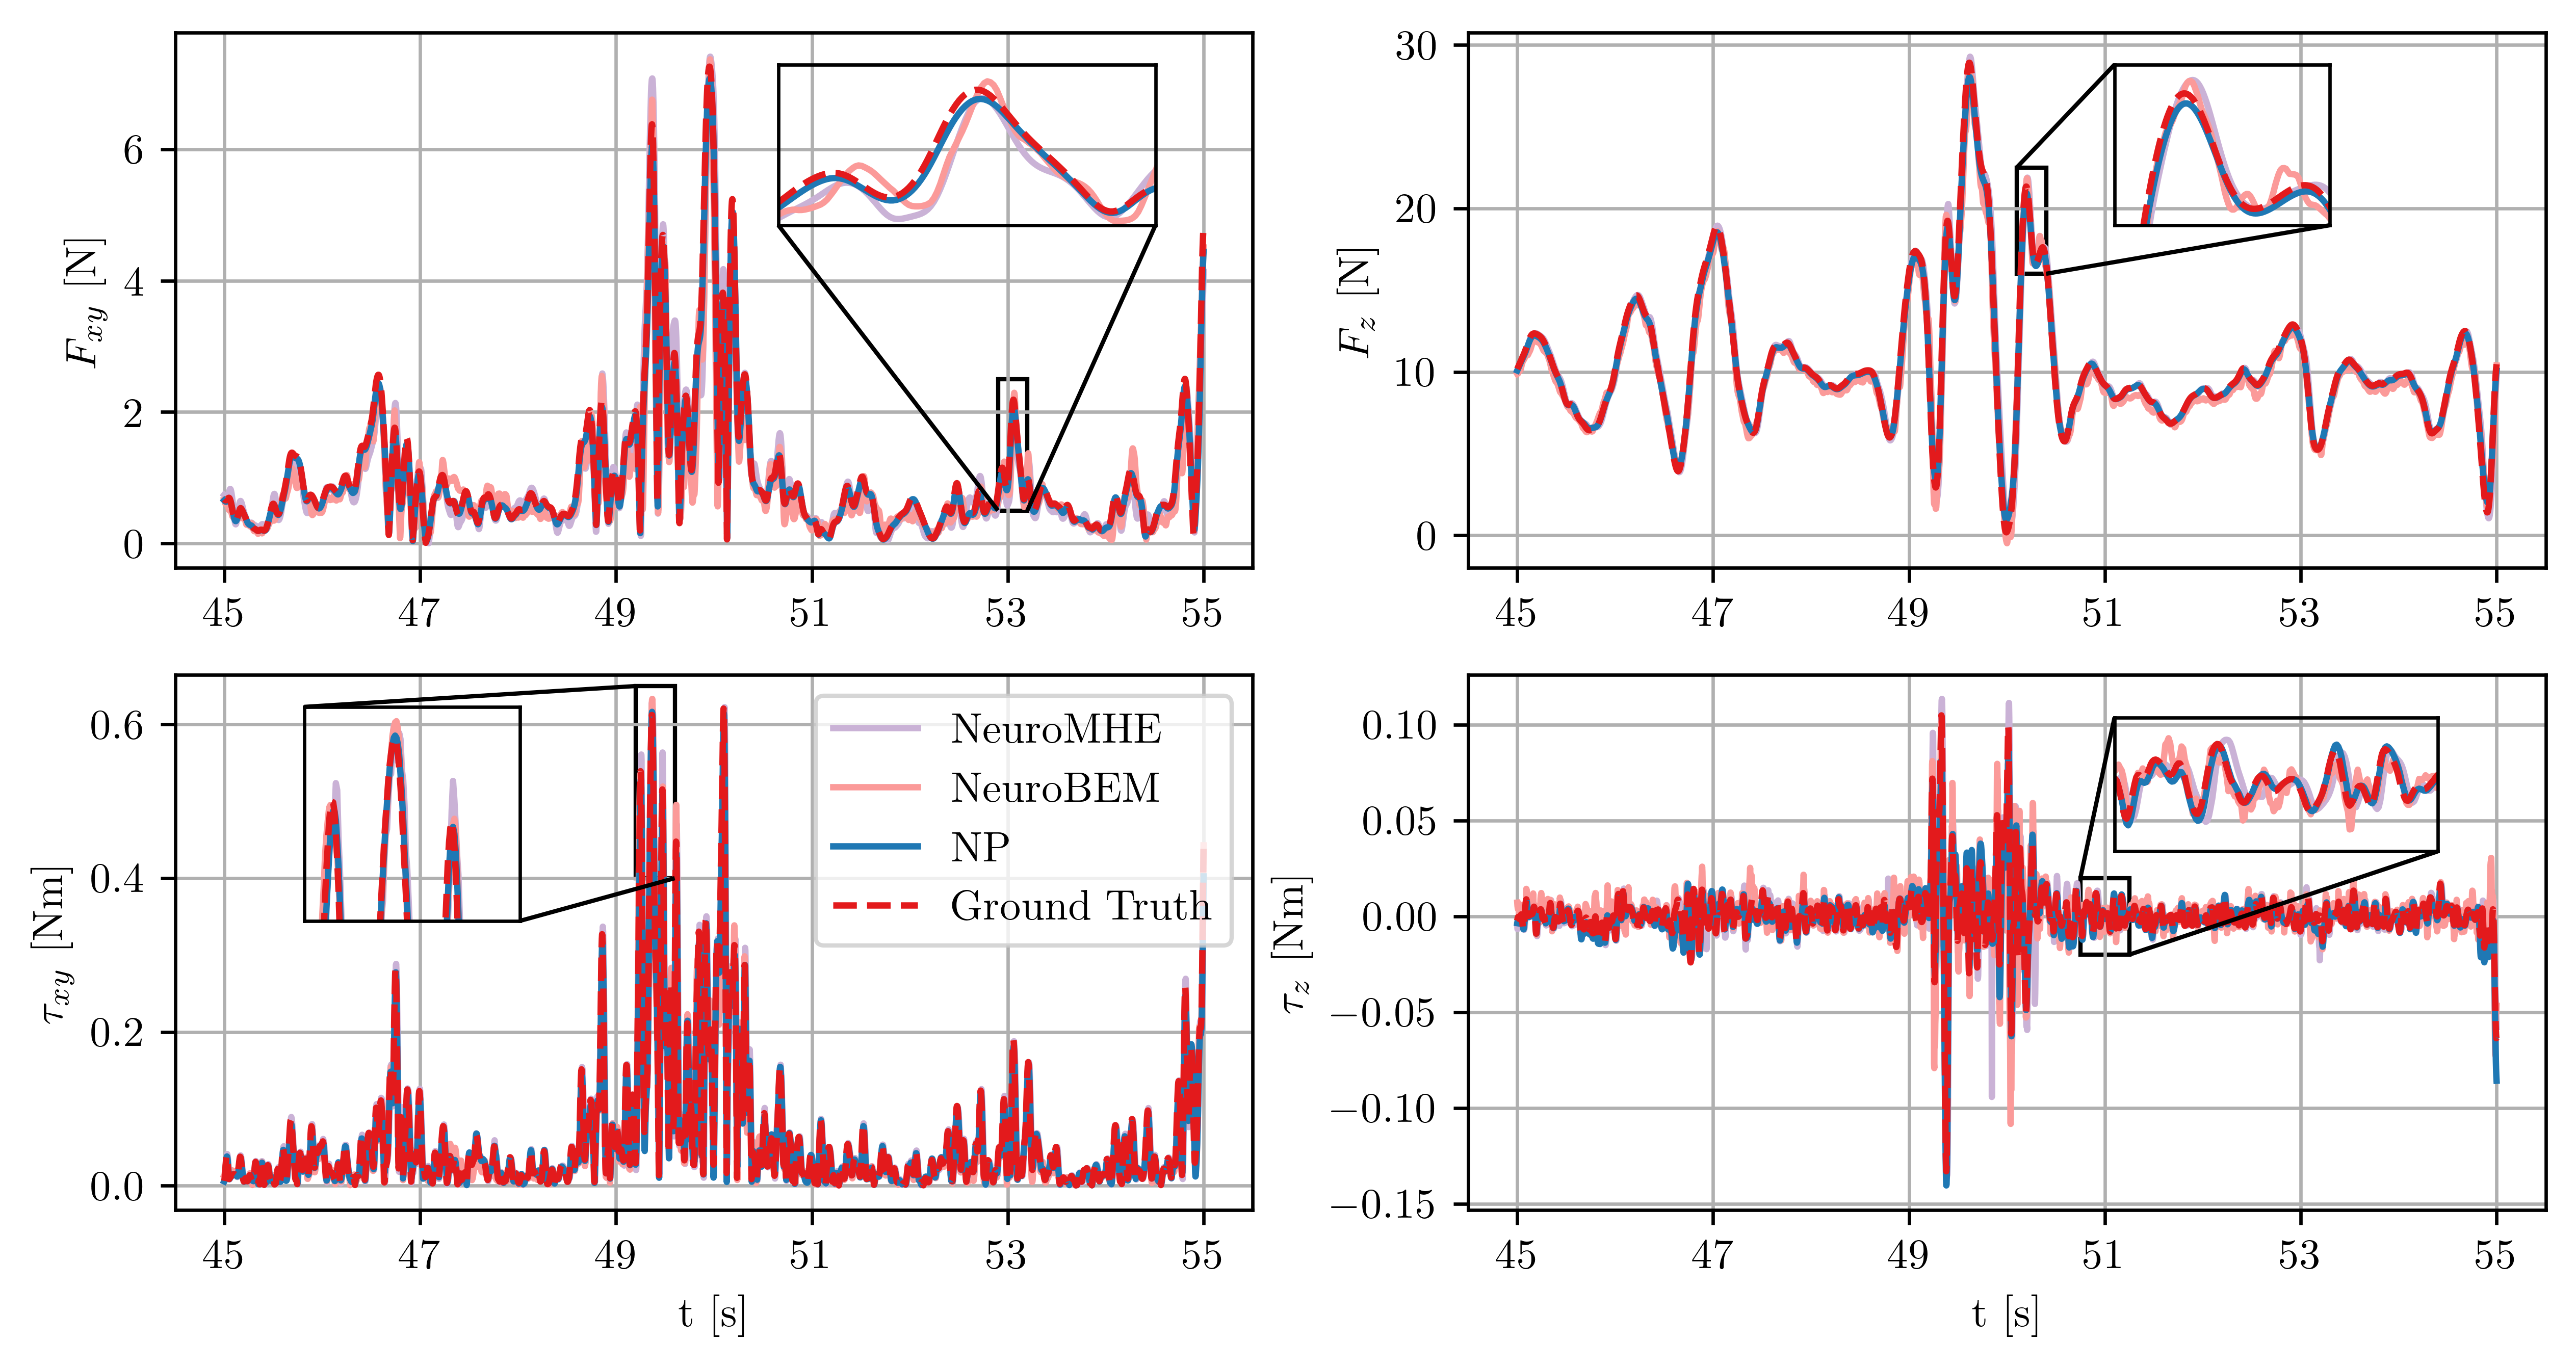
\includegraphics[width=39pc]{picture/bem_comparison.png} 
	\caption{NeuroBEM、NeuroMHE和NP的外力和力矩估计性能} 
	\label{3-5}
\end{figure}
为了验证Neural Predictor的泛化性,在6个训练数据集之外的激进飞行轨迹上评估了其性能,具体结果如\autoref{table_bem} 所示。结果表明,Neural Predictor在所有情况下均得到了更小的外力和力矩估计误差,且其表现明显优于NeuroMHE和NeuroBEM。在力估计方面,Neural Predictor在“Race track\_1”轨迹上的误差最大减少了72.06\%。在力矩估计方面,Neural Predictor在四个轨迹中明显优于NeuroMHE和NeuroBEM,在另外两个轨迹中表现相当。这些结果表明,Neural Predictor在许多未见过的激进飞行轨迹中展现出较强的泛化能力,并在外力和力矩估计方面超越了当前最先进的基于学习的估计方法。

\begin{figure}[hbt!]
	\centering
	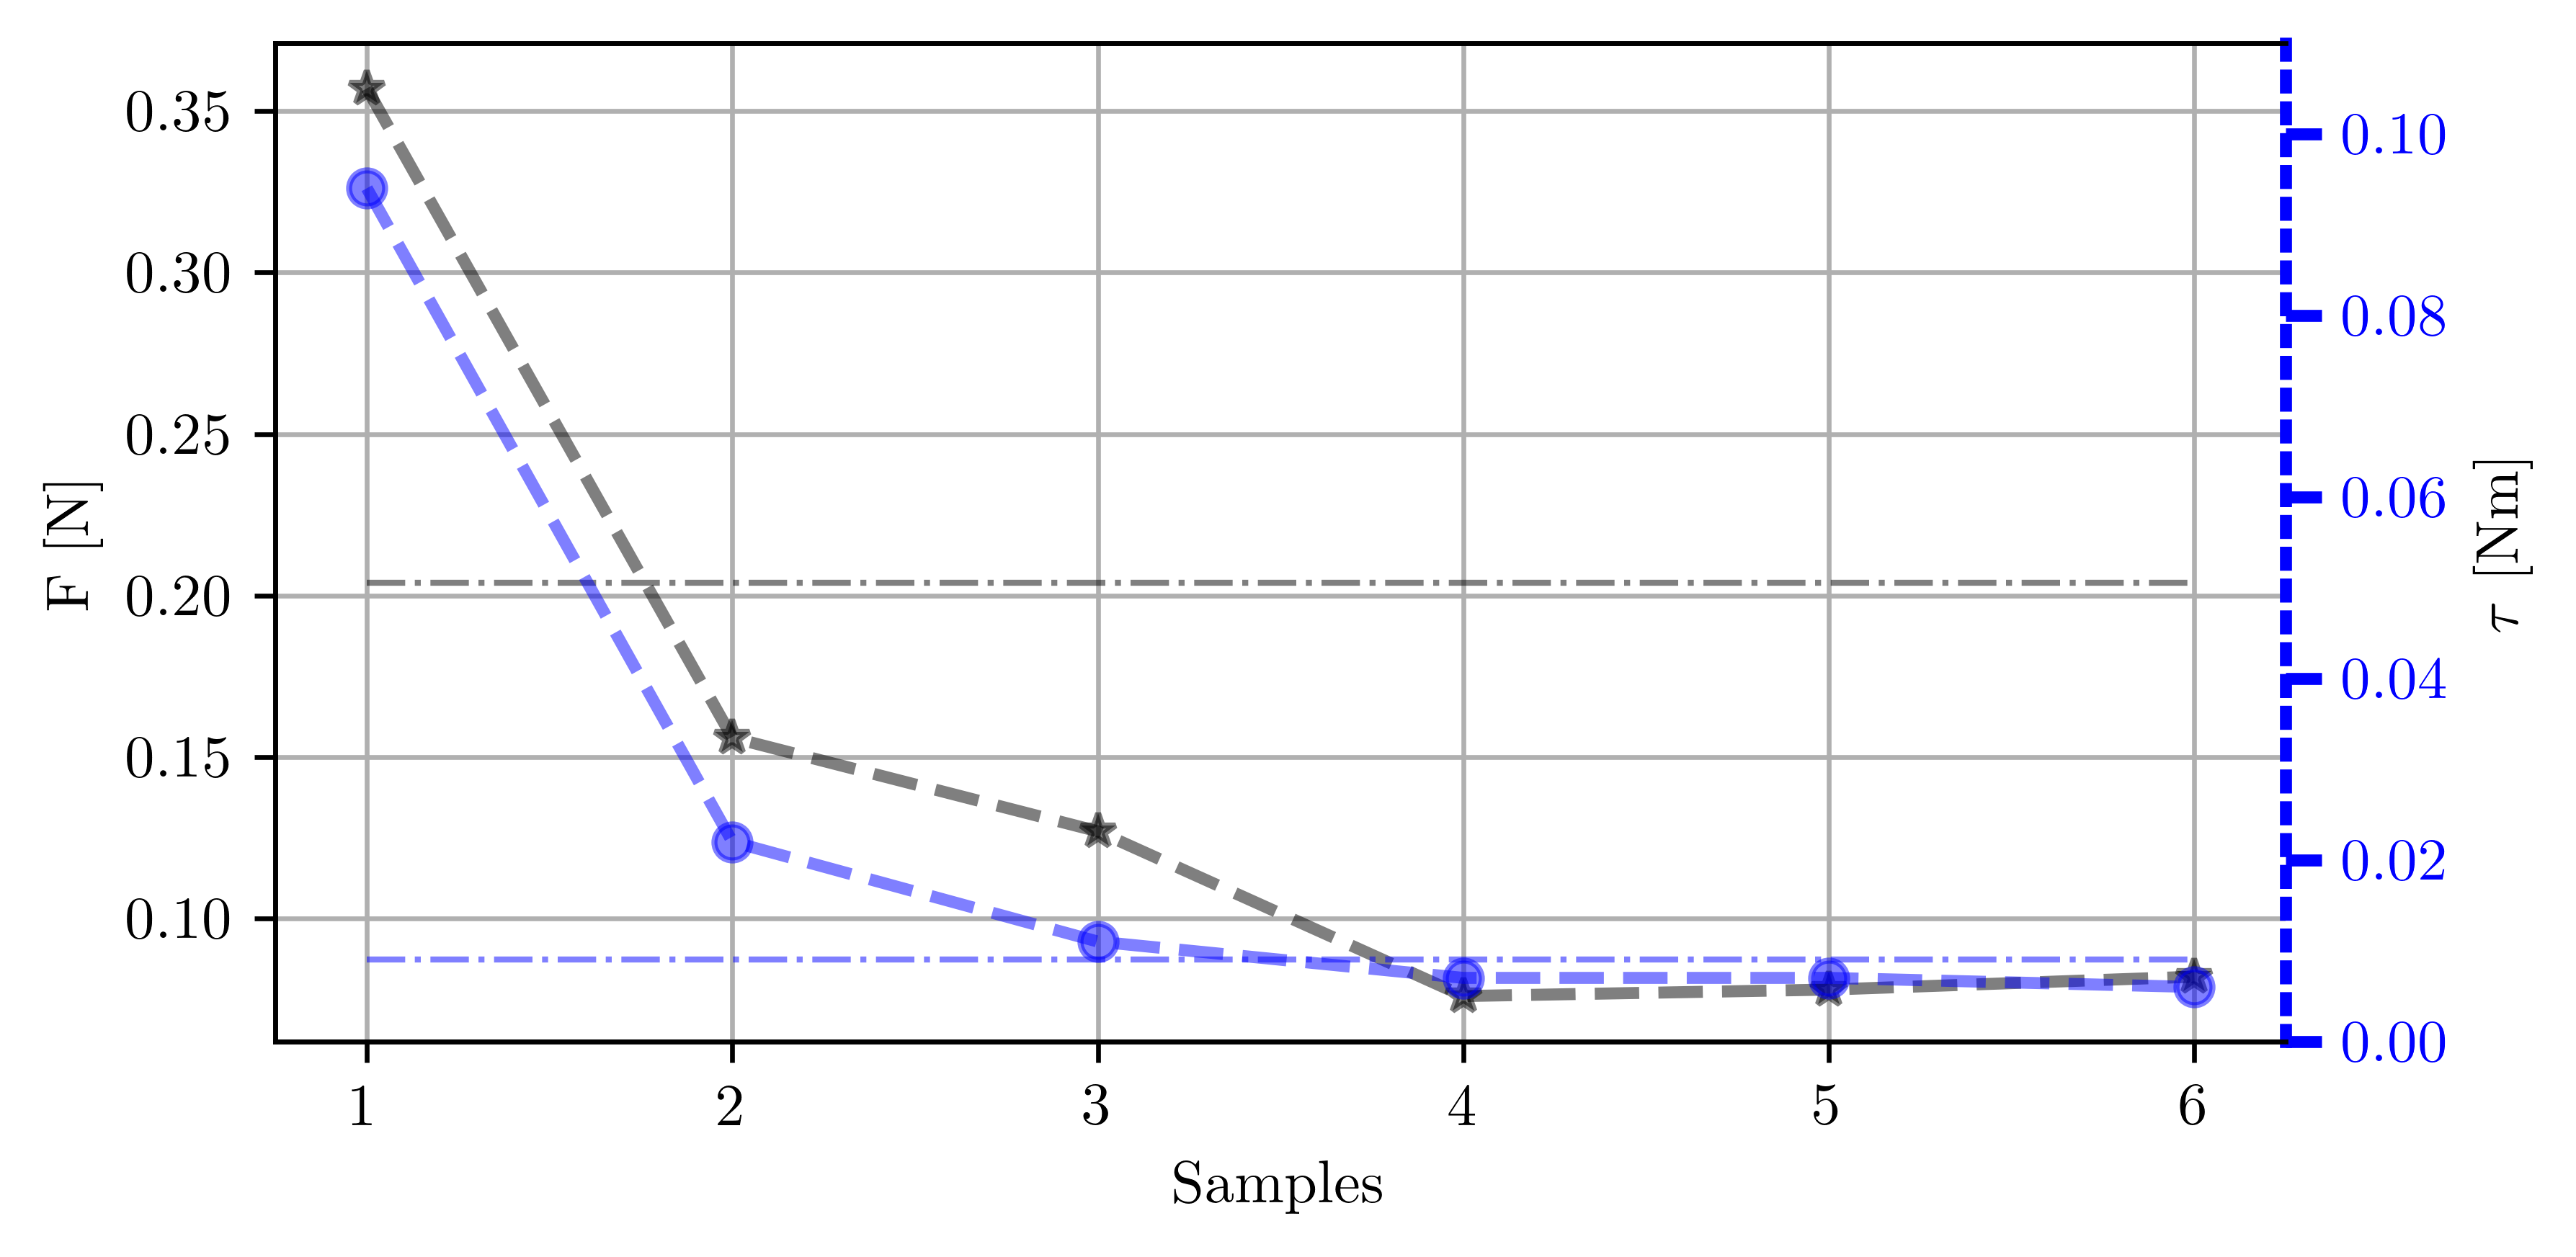
\includegraphics[width=36pc]{picture/kk/sample_efficiency.png} 
	\caption{NP在“Race track\_1”测试数据集上使用不同样本量训练后的外力和力矩的估计误差(RMSE)} 
	\label{3-6}
\end{figure}
为验证Neural Predictor的高效性,使用1000至6000个样本对其进行了训练,并在测试数据集上评估了其估计性能,结果如\autoref{3-6} 所示。从图中可以看出,随着训练样本量的增加,Neural Predictor的均方根误差逐渐降低。然而,当训练样本达到4000、5000和6000时,模型在测试集上的表现趋于一致。这表明,4000个训练样本已足够揭示外力/力矩与线速度/角速度之间的关系。此外,与使用4000个样本训练的NeuroMHE相比,Neural Predictor在样本量少于4000个的情况下仍能表现出较高的性能。具体而言,在力估计任务上,Neural Predictor仅需约1800个训练样本即可达到与NeuroMHE相当的性能,显著减少了训练所需的样本量。这些结果表明,Neural Predictor具有更高的效率,能够在较少的训练数据下实现较好的外力和力矩估计性能。

此外,尽管Neural Predictor在离线阶段进行训练,但结果表明,它在外力和力矩估计中依然具备较强的自适应能力。由于训练过程完全在离线环境中完成,Neural Predictor在在线执行阶段仅需进行前向推理,从而显著降低了机载计算设备的计算负担。
\begin{figure}[hbt!]
	\centering
	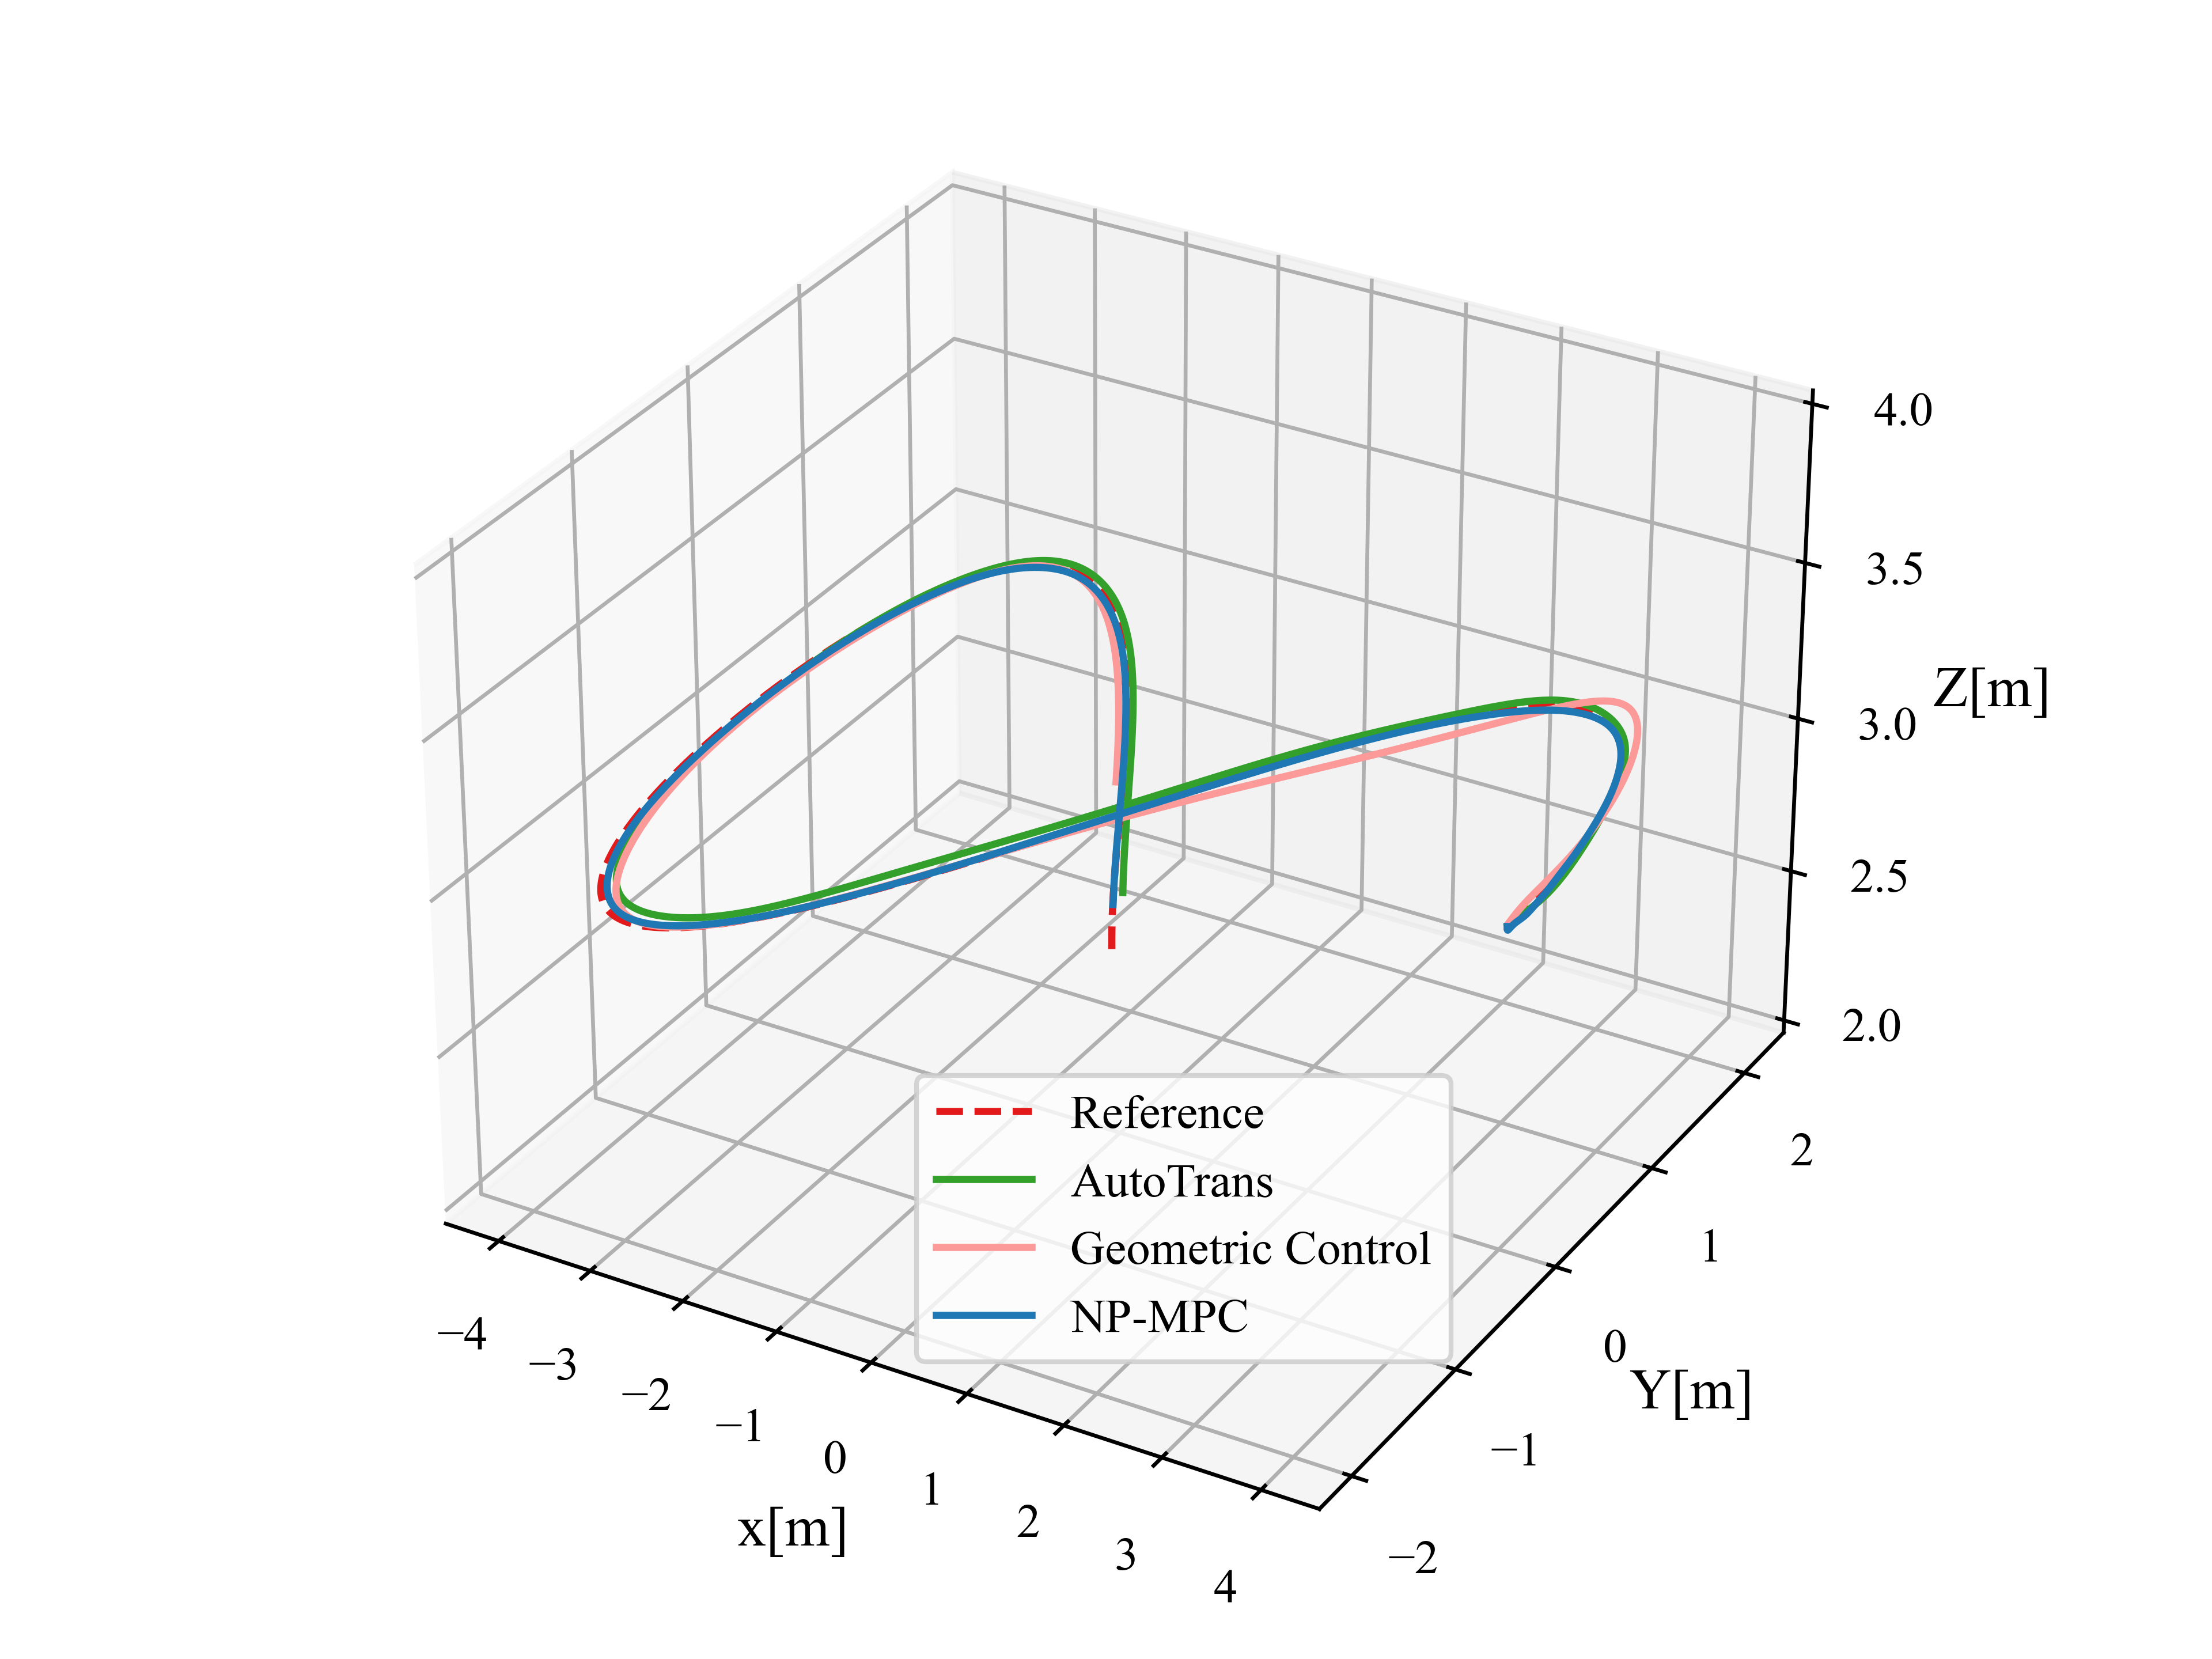
\includegraphics[width=36pc]{picture/kk/3d_trj.png} 
	\caption{三维空间下双纽线轨迹跟踪效果图} 
	\label{3-70}
\end{figure}

在闭环控制中,将训练好的 Neural Predictor集成到MPC中,形成了 NP-MPC 框架。为了全面评估 NP-MPC 的性能,仿真实验对比了三种控制方法:AutoTrans \cite{li2023autotrans}、Geometric Control\cite{sreenath2013geometric}和 NP-MPC 。在数值仿真中,从多项式轨迹生成的轨迹集中随机选择一条激进飞行的轨迹在数值仿真中进行跟踪,以验证控制策略的鲁棒性和适应性,如\autoref{3-70} 所示。仿真结果表明,NP-MPC 在轨迹跟踪方面表现出更高的精度和更快的响应速度,AutoTrans 和 Geometric Control也能对期望轨迹进行跟踪,但是和NP-MPC相比表现出不同程度的偏差和滞后。

NP-MPC 的优势不仅体现在更强的实时适应性和控制精度上,同时在动态复杂环境下也表现出更强的鲁棒性和泛化能力。这主要归功于 Neural Predictor 的引入,使得系统能够更准确地捕捉和预测无人机吊运系统的复杂动力学特性,从而在轨迹跟踪任务中实现更优的控制效果。


\section{本章总结}
本章提出了一种基于数据驱动的学习方法——Neural Predictor,用于捕捉无人机绳系吊运系统中由载荷引起的外力和力矩。Neural Predictor的核心观点是利用Koopman算子理论,将外力和力矩建模为一个动态系统,并用Lipschitz常数从理论上保证了预测误差的界限。与现有的最优的估计方法相比,Neural Predictor具有响应速度快、泛化能力强、效率高以及外力和力矩估计更准确的优势。此外,将 Neural Predictor 与模型预测 控制框架相结合,形成 NP-MPC,可以显著提升闭环跟踪性能。值得注意的是,Neural Predictor还可以与其他基于模型的控制器例如MPC结合,进而提高其闭环性能。
% 在第五章的,将Neural Predictor与模型预测控制框架相结合,形成NP-MPC,可以显著提升闭环跟踪性能。



\cleardoublepage

\chapter{基于数据驱动的多无人机吊运控制}
\chaptermark{基于数据驱动的多无人机吊运控制}
针对载荷已知的多无人机绳系吊运系统,控制精度和系统稳定性在实际应用中往往面临巨大的挑战。特别是在复杂环境下,如载荷的动态变化、外部扰动的干扰、以及无人机间的协同与相互影响。传统的控制方法大多依赖于手动调参,需要进行人工干预且调参过程复杂,难以适应动态变化的环境。本章的目标是设计一种方法,用于提升多无人机绳系吊运系统的自适应调节能力。具体而言,本章进行了如下研究:

(1)通过分布式模型预测控制对多无人机绳系吊运系统进行控制,实现所有无人机和载荷的轨迹跟踪,同时确保运输过程中载荷姿态的稳定性。每架无人机和载荷配备独立的模型预测控制器,将其它无人机和载荷带来的影响统一视为外部信号,并在考虑到全局协调的情况下进行局部优化。

(2)通过分布式灵敏度传播算法高效并行计算闭环状态对MPC超参数的灵敏度。该算法的创新在于通过分布式计算模式,使得每个无人机能够独立高效地评估其对MPC超参数的状态灵敏度,进而加速了系统的实时响应。

(3)提出了一种自适应学习的超参数优化算法——Autotune,自动调节多无人机绳系吊语系统中的各种MPC超参数,其中所有超参数均通过深度神经网络(DNN)表示。引入了分布式灵敏度传播算法,充分利用了多无人机系统中的动态耦合特性,并行计算无人机上的梯度。在此基础上,使用分布式策略梯度学习算法生成归一化超参数,并整合到分布式模型预测控制框架中,从而实现了控制器的实时动态适应能力。

\section{问题描述}
本文考虑 $n$ 架无人机协同运输一个载荷,吊挂载荷通过 $n$ 根等长系绳与$n$ 架无人机相连。
% 可以通过对第3章的数据驱动的模型预测控制算法进行延伸,应用到本章的多无人机绳系吊运系统中。

在多无人机系统中,控制策略通常分为集中式和分布式两类。集中式控制由中央控制器协调和管理所有无人机,而分布式控制让每架无人机根据局部信息和相邻无人机的状态独立决策。本章重点研究一种完全分布式的控制方法,以避免集中式控制对单一控制中心的依赖。

在实际操作中,多无人机系统的超参数数量庞大且动态耦合,使手动调节复杂且低效。首先,随着无人机数量的增加,超参数的数量也随之增长,调节过程更加复杂;其次,由于系绳连接导致无人机间存在动态耦合,这种效应在载荷具有非均匀质量分布或执行激进飞行任务时尤为显著。在此类场景下,无人机间的拉力分配往往不均衡且动态变化,需要MPC动态调整耦合权重。此外,MPC 的参考轨迹需随环境和系统状态变化动态调整,以避免载荷与障碍物发生碰撞。

本章要解决的问题是,利用基于数据驱动的自适应学习超参数优化方法,在线动态调整分布式闭环MPC算法的参数权重。这些权重在无人机间实现最优构型分配,有效确保了多无人机与吊挂载荷的稳定。
% 在多无人机绳系吊运系统对于给定的任务路径,控制载荷
% 对于多无人机绳系吊运系统,可以对整个
% 将第3章的数据驱动的模型预测控制方法包含在一个集中式 MPC 框架
% 在本章中,

\section{多无人机模型预测控制方法}
本章继续采用模型预测控制方法,设计多无人机绳系吊运系统的运动控制策略,目标是使所有无人机和载荷跟踪设定好的期望轨迹,同时在运输过程中保持载荷姿态的稳定性。在本小节,先对多无人机的集中式模型预测控制策略和分布式模型预测控制策略作简要介绍。
\subsection{集中式模型预测控制}
集中式模型预测控制(Centralized MPC)是一种以全局优化为目标的控制策略,适用于多无人机系统的运动控制和路径规划。集中式MPC能够通过全局优化的方式有效协调多个无人机之间的相互关系,解决多无人机系统中的耦合问题,确保系统的整体性能,从而为系统生成最优的状态轨迹。


设第 \( i \) 个无人机的状态为 
\(
\bm{x}_i = \left[ \bm{p}_i, \bm{v}_i, \bm{q}_i, \bm{\omega}_i \right] \in \mathbb{R}^{13}
\),
控制输入为 
\(
\bm{u}_i = \left[ f_i, \bm{\tau}_i \right] \in \mathbb{R}^4
\),
载荷的状态为 
\(
\bm{x}_l = \left[ \bm{p}_l, \bm{v}_l, \bm{q}_l, \bm{\omega}_l \right] \in \mathbb{R}^{13}
\),
载荷的虚拟控制输入为 
\(
\bm{u}_l = \left[ \bar{T}_1, \cdots, \bar{T}_n \right] \in \mathbb{R}^n
\),$\mathcal{I}_q = \{1, \cdots , n\}$ 表示无人机的索引集合。
在MPC框架中,拉力大小$\bar{T}_i$并不直接并不直接用于系统控制,因为它会使系统模型具有混合特性,从而增加优化问题的复杂性,导致求解更加困难。它仅作为虚拟控制输入,在模型预测控制的计算过程中使用。该拉力值通过第3章提出的Neural Predictor进行优化计算得到。

集中式MPC的代价函数由无人机和载荷的代价函数组成。每个无人机的代价函数采用二次形式,用于惩罚无人机状态和控制与参考值之间的偏差。单个无人机的代价函数表示为:
\begin{equation}
	J_i = \frac{1}{2}\sum_{k=0}^{N-1}\left(\bar{\boldsymbol{x}}_{i,k}^\mathrm{T}\boldsymbol{Q}_{x_i}\bar{\boldsymbol{x}}_{i,k}+\bar{\boldsymbol{u}}_{i,k}^\mathrm{T}\boldsymbol{R}_{x_i}\bar{\boldsymbol{u}}_{i,k}\right)+\frac{1}{2}\bar{\boldsymbol{x}}_{i,N}^\mathrm{T}\boldsymbol{P}_{x_i}\bar{\boldsymbol{x}}_{i,N}
	\label{juav}
\end{equation}
其中,$N$ 是预测时域,$\bar{\boldsymbol{x}}_{i,k}$ 和$\bar{\boldsymbol{u}}_{i,k}$ 是时间 $k$ 时刻无人机 $i$ 的预测状态和控制输入,$\boldsymbol{Q}_{x_i}$ 和 $\boldsymbol{R}_{x_i}$ 是无人机$i$ 的状态和控制输入的权重矩阵,$\boldsymbol{P}_{x_i}$ 是无人机$i$ 的终端状态的权重矩阵。

载荷的代价函数与 \( J_i \) 形式相同,定义为:
\begin{equation}
    J_i = \frac{1}{2}\sum_{k=0}^{N-1}\left(\bar{\boldsymbol{x}}_{l,k}^\mathrm{T}\boldsymbol{Q}_{x_l}\bar{\boldsymbol{x}}_{l,k}+\bar{\boldsymbol{u}}_{l,k}^\mathrm{T}\boldsymbol{R}_{x_l}\bar{\boldsymbol{u}}_{l,k}\right)+\frac{1}{2}\bar{\boldsymbol{x}}_{l,N}^\mathrm{T}\boldsymbol{P}_{x_l}\bar{\boldsymbol{x}}_{l,N}
	\label{jpayload}
\end{equation}
其中$\bar{\boldsymbol{x}}_{l,k}$ 和$\bar{\boldsymbol{u}}_{l,k}$ 是时间 $k$ 时刻载荷的预测状态和控制输入,$\boldsymbol{Q}_{x_i}$ 和 $\boldsymbol{R}_{x_i}$ 是载荷的状态和控制输入的权重矩阵,$\boldsymbol{P}_{x_i}$ 是载荷的终端状态的权重矩阵。


基于上述定义,可以将多无人机系统集中式模型预测控制问题表述为:
\begin{equation}
	\begin{aligned} 
	&\operatorname*{minimize}_{\bm{X}, \bm{U}}& & J_l(\bm{X}_l, \bm{U}_l) + \sum_{i=1}^n J_i(\bm{X}_i, \bm{U}_i)  \\
	&\text{subject to}& & \begin{aligned}
	& \bm{x}_{i,k+1} = \bar{\bm{f}}_i^k(\bm{x}_{i,k}, \bm{u}_{i,k}, \Delta t; \bm{x}_{l,k}, \bm{u}_{l,k}), \quad \forall i \in \mathcal{I}_q \\
	& \bm{x}_{l,k+1} = \bar{\bm{f}}_l^k(\bm{x}_{l,k}, \bm{u}_{l,k}, \Delta t; \bm{x}_{1,k}, \cdots, \bm{x}_{n,k}) \\
	& \bm{x}_{i,0} = \bm{x}_{i,t}, \quad \forall i \in \mathcal{I}_q \\
	& \bm{x}_{l,0} = \bm{x}_{l,t} \\
	& \bm{u}_{i}^{\min} \leq \bm{u}_{i,k} \leq \bm{u}_{i}^{\max}, \quad \forall i \in \mathcal{I}_q \\
	& 0 < \bar{T}_i \leq \bar{T}_{\max}, \quad \forall i \in \mathcal{I}_q \\
	& \|\bm{p}_{i,k} - \bm{p}_{l,k} - \bm{R}_{l,k} \bm{r}_i\|^2 = l_0, \quad \forall i \in \mathcal{I}_q \\
	& 2d_\text{quad} - \|\bm{p}_{i,k} - \bm{p}_{j,k}\|^2 < 0, \quad \forall i, j \in \mathcal{I}_q, i \neq j \\
	& d_\text{quad} + d_\text{obs} - \|\bm{p}_{i,k} - \bm{p}_\text{obs}\|^2 < 0, \quad \forall i \in \mathcal{I}_q \\
	& d_\text{load} + d_\text{obs} - \|\bm{p}_{l,k} - \bm{p}_\text{obs}\|^2 < 0        
	\end{aligned}	
\end{aligned}
\label{multimpc}
\end{equation}

其中,\( \bm X_i = \left[ \bm x_{i,0}, \cdots, \bm x_{i,N} \right] \) 和 \( \bm X_l = \left[ \bm x_{l,0}, \cdots, \bm x_{l,N} \right] \) 分别表示第 \( i \) 个无人机和载荷的长度为 \( N+1 \) 的状态轨迹,
\( \bm U_i = \left[ \bm u_{i,0}, \cdots, \bm u_{i,{N-1}} \right] \) 和 \( \bm U_l = \left[ \bm u_{l,0}, \cdots, \bm u_{l,{N-1}} \right] \) 表示相应的控制轨迹,\( \bm X \) 和 \( \bm U \) 是整个系统的状态与控制轨迹集合。
式 (\ref{multimpc}) 中的约束从上到下分别为:
无人机与载荷的离散动态方程和初始条件;
无人机的控制约束;
系绳拉力约束;
系绳长度约束;
无人机之间的安全距离约束;
无人机和载荷的障碍物避障约束。

\subsection{分布式模型预测控制}
集中式模型预测控制问题的计算复杂度较高,并且对通信带宽和系统可靠性要求较高,这使得其在多无人机绳系吊运系统中扩展性较差,难以满足实时性的需求。本文提出了一种分布式的模型预测控制方法,该方法通过将\autoref{multimpc} 分解到各个无人机和载荷中实现并行计算,从而降低计算复杂度并提高系统的扩展性。

在设计分布式MPC时,需要进一步分析式 (\ref{multimpc}) 中的若干特性。首先,载荷与无人机的状态和控制变量之间没有直接耦合,集中式MPC中的代价函数在各个无人机和载荷之间是可分离的;此外,各个无人机之间的动力学通过系绳拉力(即载荷状态和控制变量的函数)和系绳长度约束间接耦合,而无人机状态之间的耦合仅通过安全距离约束体现。这些特点为分布式优化提供了理论依据。

基于上述分析,可以通过将其它无人机的MPC状态轨迹视为外部信号来对问题进行分解,在每个无人机进行MPC的开环预测时,其他无人机的状态轨迹保持不变。分布式MPC方法通过独立更新所有无人机和载荷的状态轨迹直到收敛,从而实现对多无人机绳系吊运系统的控制。

\textbf{注4.1:}为了有效提升收敛性,将式 (\ref{multimpc}) 中的约束条件转化为软约束,并引入到代价函数中。可以使用障碍函数来表示软约束,障碍参数 $\gamma > 0$ 用于控制约束满足程度和计算效率之间的权衡,当障碍参数足够小的时候,软约束可以逼近原始约束。


具体而言,对于第 $i$ 个无人机,其它无人机的状态轨迹 $ \bm X_j, \forall j \neq i$、载荷的状态轨迹 $\bm X_l$ 和 载荷的输入轨迹$\bm U_l$ 都被视为该无人机的外部信号,在开环预测过程中保持不变,分解后的MPC问题定义如下:

\begin{equation}
	\begin{aligned} 
	&\operatorname*{minimize}_{\bm{X}_i, \bm{U}_i} & & J_i + \sum_{k=0}^{N} \left( \frac{1}{2\gamma} h_{i,k}{}^2 - \gamma \sum_{j \neq i} \ln(-g_{j,k}) -\gamma \ln(-g_{{o-i},k}) \right)\\
	&\text{subject to}& & \begin{aligned}
& \bm{x}_{i,{k+1}} = \bar{f}_{i,k}(\bm{x}_{i,k}, \bm{u}_{i,k}, \Delta t; \bm{x}_{l,k}, \bm{u}_{l,k}) \\
& \bm{x}_{i,0} = \bm{x}_{i,t}\\
& \bm{u}_{i,{\text{min}}} \leq \bm{u}_{i,k} \leq \bm{u}_{i,{\text{max}}}		\end{aligned}	
\end{aligned}
\label{multiuav}
\end{equation}
其中
$\gamma \in \mathbb{R}^+$ 为障碍参数,$\bm p_{l-i}$ 表示载荷与无人机 $i$ 之间的相对位置。
$h_{i,k} = \|\bm p_{l-i}\|^2 - l_0$为系绳长度约束,
$g_{j,k} = 2d_{\text{quad}} - \|\bm p_{i,k} - \bm p_{j,k}\|^2$为无人机之间的安全间距约束,$g_{{o-i},k} = d_{\text{quad}} + d_{\text{obs}} - \|\bm p_{i,k} - \bm p_{\text{obs}}\|^2$为无人机$i$的避障约束。

对于载荷的分解MPC问题,无人机的状态轨迹 $\bm X_i, \forall i \in \mathcal{I}_q$ 被视为载荷的外部信号。MPC问题定义如下,

\begin{equation}
	\begin{aligned} 
	&\operatorname*{minimize}_{\bm{X}_l, \bm{U}_l}& &  J_l + \sum_{k=0}^{N} \left( \frac{1}{2\gamma} \sum_{i=1}^{n} h_{i,k}{}^2 - \gamma \ln(-g_{{o-l},k}) \right)\\
	&\text{subject to}& & \begin{aligned}
& \bm{x}_{l,{k+1}} = \bar{f}_{l,k}(\bm{x}_{l,k}, \bm{u}_{l,k}, \Delta t; \bm{x}_{1,k}, \cdots, \bm{x}_{n,k}) \\
& \bm{x}_{l,0} = \bm{x}_{l,t}\\
& 0 < \bm{u}_{l,k} \leq \bar{T}_{\text{max}}, \forall i \in \mathcal{I}_q		\end{aligned}	
\end{aligned}
\label{multipayload}
\end{equation}

其中$g_{{o-l},k} = d_{\text{load}} + d_{\text{obs}} - \| \bm p_{l,k} - \bm p_{\text{obs}}\|^2$为载荷的避障约束。



分布式MPC由式 (\ref{multiuav}) 和式 (\ref{multipayload}) 组成,通过迭代方式进行求解。设第 $k$ 次迭代时的轨迹为 $\bm X_{i,k}, \bm U_{i,k}, \bm X_{l,k}, \bm U_{l,k}$,在每个采样时刻 $t$,给定初始条件 $\bm X_{i,0}, \forall i \in \mathcal{I}_q, \bm X_{l,0}, \bm U_{l,0}$,首先为每个无人机求解式 (\ref{multiuav}),然后使用更新后的轨迹 $\bm X_{i,1}, \forall i \in \mathcal{I}_q$ 求解问题式 (\ref{multipayload}) 以获得载荷的轨迹。这个过程会持续迭代,直到所有无人机的轨迹误差 $\bm X_i^k - \bm X_i^{k-1}$ 和控制输入误差 $\bm U_i^k - \bm U_i^{k-1}$ 满足预定的阈值 $\delta \in \mathbb{R}^+$。

图 \ref{4_2} 进一步清晰地展示了解决分布式MPC问题中的数据交换过程(即在一个无人机的MPC问题中,将其他无人机的状态轨迹视为外部信号)。由于载荷缺乏计算能力,系统会从无人机中随机选择一个无人机作为“中央无人机”来求解\autoref{multiuav} 和\autoref{multipayload}。
分布式MPC的流程如算法 \ref{alg:mpc_multilift} 所示。

\begin{figure}[H]
	\centering
	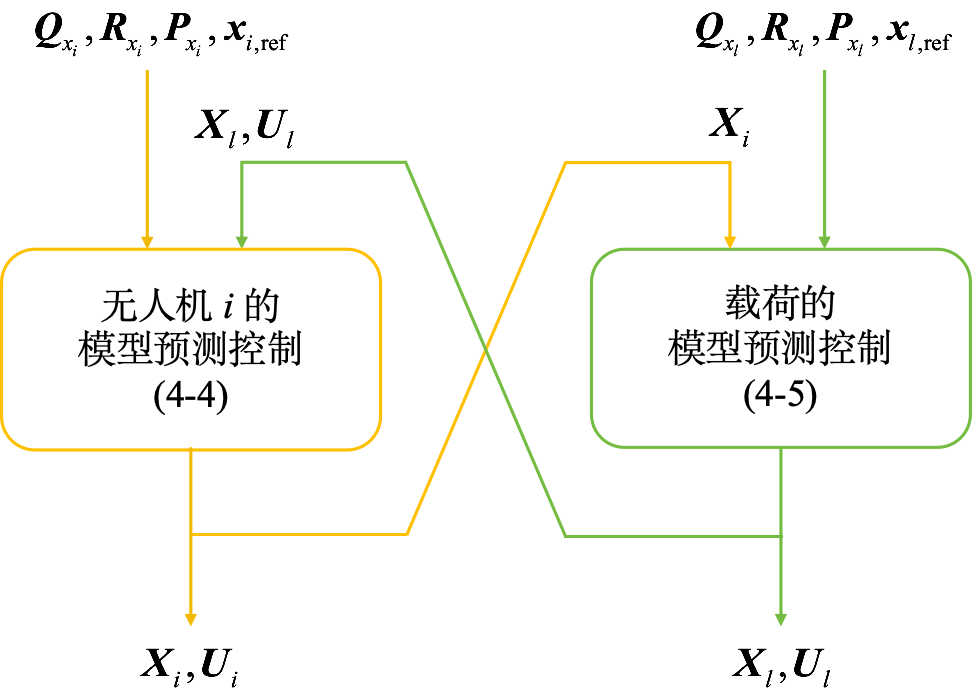
\includegraphics[width=24pc]{picture/4_2.png} 
	\caption{分布式MPC中数据交换与迭代过程示意图
	} 
	\label{4_2}
\end{figure}
\begin{algorithm}[H]
	\captionsetup{font={stretch=1.2}}
    \linespread{1.2}\selectfont % 设置行距为1.2倍
	\caption{多无人机的分布式MPC}
	\label{alg:mpc_multilift}
	\textbf{输入:} 阈值 $\delta$,最大迭代次数 $k_{\text{max}}$,以及初始条件 $\bm{X}_{i,0}$,$\bm{U}_{i,0}$,$\bm{X}_{l,0}$ 和 $\bm{U}_{l_0}$。\\
	\textbf{输出:} 状态轨迹 $\bm{X}_i$ 和控制输入轨迹 $\bm{U}_i$,$\forall i\in\mathcal{I}_{A}$。
	
	\begin{algorithmic}[1]
	\State $k \gets 1$
	\While{$e \geq \delta$ $and$ $k \leq k_{\text{max}}$}
		\For{$i \gets 1$ \textbf{to} $n$ ($in$ $parallel$)}
			\State  基于外部轨迹 $\bm{X}^j_{k-1}, \forall j \in \mathcal{I}_q, j \neq i$, $\bm{X}^l_{k-1}$ 和 $\bm{U}^l_{k-1}$ 求解\autoref{multiuav} 计算 $\bm{X}_i$ 和 $\bm{U}_i$;
			\Statex \quad \quad  $\triangleright$ 在每个无人机上运行并发送到“中央无人机”
		\EndFor
		\State 更新无人机轨迹: $\bm{X}_{i,k} \gets \bm{X}_i$ 和 $\bm{U}_{i,k} \gets \bm{U}_i, \forall i \in \mathcal{I}_q$;
		\State 通过 $\bm{X}_{i,k}, \forall i \in \mathcal{I}_q$ 求解\autoref{multipayload} 计算 $\bm{X}_l$ 和 $\bm{U}_l$
		\State 更新载荷轨迹: $\bm{X}_{l,k} \gets \bm{X}_l, \bm{U}_{l,k} \gets \bm{U}_l$;
		\Statex \quad \quad $\triangleright$ 在“中央无人机”中运行
		\State 计算误差: $e \gets \max \{ e_{\bm{X}_i}, e_{\bm{U}_i} \}, \forall i \in \mathcal{I}_A$ ,
		\Statex \quad \quad 其中 $e_{\bm{X}_i} = \frac{1}{N} \| \bm{X}_{i,k} - \bm{X}_{i,{k-1}} \|_2, e_{\bm{U}_i} = \frac{1}{N} \| \bm{U}_{i,k} - \bm{U}_{i,{k-1}} \|_2$;
		\State 更新迭代次数: $k \gets k + 1$;
	\EndWhile
	\end{algorithmic}
\end{algorithm}
\section{自适应学习的超参数优化}
分布式MPC通过对\autoref{multimpc} 中的集中式MPC算法进行近似来提高计算效率,如算法\ref{alg:mpc_multilift} 所示。随着阈值\(\delta\) 的减小和最大迭代\(k_{\text{max}}\)的增加,近似的准确性会得到提升。然而,算法\ref{alg:mpc_multilift} 的性能(包括预测轨迹的可行性和跟踪精度)依赖于对多种超参数的精细调整。这些超参数包括权重矩阵的选择以及参考轨迹在\autoref{juav} 和\autoref{jpayload} 中的设计。

令 \(\bm \theta_i \in \mathbb{R}^{m_i}, \forall i \in \mathcal{I}_q\) 表示第 \(i\) 个无人机的超参数,\(\bm \theta_l \in \mathbb{R}^{m_l}\) 表示载荷的超参数。
% 因此,可以将分解后的 MPC 问题参数化为无人机的MPC和载荷的MPC。
要实现动态耦合的MPC权重的调节,仅通过独立调节各个无人机和载荷的 MPC 超参数是不太可能的,单一固定的超参数无法在各种场景下普遍适用于所有无人机。本节提出了Autotune框架,用于自动调节多无人机绳系吊运系统中的超参数。该框架通过深度神经网络生成自适应MPC超参数,在分布式灵敏度传播方法的基础上,用分布式策略梯度算法优化控制参数,实现自适应学习。

\subsection{超参数自适应调节方法}
考虑一个离散时间的动力学系统:
\begin{equation}
    \bm x_{k+1} = f(\bm x_k, \bm u_k)
	\label{1}
\end{equation}
其中 \( \bm x_k \in \mathbb{R}^n \) 和 \( \bm u_k \in \mathbb{R}^m \) 分别是状态和控制,初始状态 \( \bm x_0 \) 是已知的。  
控制由反馈控制器生成,用来追踪目标状态 \( \bm x_{t,\text{ref}} \in \mathbb{R}^n \),其表达式为:
\begin{equation}
    \bm u_k = h(\bm x_k, \bm x_{k,\text{ref}}, \bm \theta)
	\label{2}
\end{equation}
其中 \( \bm \theta \in \bm \Theta \) 表示控制器的参数,\( \bm \Theta \) 是一个可行的参数集合。  
假设状态 \( {\bm x}_k \) 可以直接测量或者使用状态估计方法得到,且式(\ref{1}) 和式 (\ref{2}) 是可微的,即雅可比矩阵$\bm \nabla_{\bm x} T$, $\ \bm \nabla_{\bm u} T$, $\ \bm \nabla_{\bm x} h$ 和 $\ \bm \nabla_{\bm \theta} h$
都存在,这一假设适用于一类系统。

控制器的调参过程可以表述为以下参数优化问题:
\begin{equation}
	\label{5}
	\begin{aligned} 
		&\operatorname*{minimize}_{\bm \theta \in \bm \Theta} & & L(\bm x_{1:N}, \bm x_{{1:N},\text{ref}}, \bm u_{0:N-1}; \bm \theta) \\
		&\text{subject to} & & \begin{aligned}
			&\boldsymbol{x}_{{k+1}} = {{T}}\left(\boldsymbol{x}_{k}, \boldsymbol{u}_{{k}}\right) \\
			&\bm u_k = h(\bm x_k, \bm x_{k,\text{ref}}, \bm \theta), k \in \{0,1,...,N-1 \}
		\end{aligned} \\
	\end{aligned}
\end{equation}

本节将使用简写符号 \( L \) 来表示代价函数。对于上述优化问题,可通过梯度下降算法迭代更新学习参数:
\begin{equation}
    \bm \theta\leftarrow\mathcal{P}_{\bm \Theta}(\bm \theta-\alpha\nabla_{\bm \theta}L).
\end{equation}

为了获得代价函数 $L$ 关于参数 $\bm \pi$ 的梯度 $\nabla_{\bm \pi} L$,使用链式法则推导如下:

\begin{equation}
    \nabla_{\bm \theta} L = \sum_{k=1}^{N} \frac{\partial L}{\partial \bm x_k} \frac{\partial \bm x_k}{\partial \bm \theta} + \sum_{k=0}^{N-1} \frac{\partial L}{\partial \bm u_k} \frac{\partial \bm u_k}{\partial \bm \theta}
\end{equation}

由于一旦选择了代价函数 
$L$ ,可以确定${\partial L}/{\partial \bm x_k}$ 和 ${\partial L}/{\partial \bm u_k}$。为了进一步计算灵敏度状态 ${\partial \bm x_k}/{\partial \bm \theta}$ 和 ${\partial \bm u_k}/{\partial \bm \theta}$,可以使用灵敏度传播方法进行计算,其形式如下:

\begin{equation}
	\begin{gathered}
		\frac{\partial \bm x_{k+1}}{\partial \bm \theta} = ({\nabla}_{\bm x_k}  T + {\nabla}_{\bm u_k} T {\nabla}_{\bm x_k} h) \frac{\partial \bm x_k}{\partial \bm \theta} + {\nabla}_{\bm u_k} T {\nabla_{\bm \theta}} h\\
		\frac{\partial \bm u_k}{\partial \bm \theta} = {\nabla}_{\bm x_k} h \frac{\partial \bm x_k}{\partial \bm \theta} + {\nabla_{\bm \theta}} h
	\end{gathered}
\end{equation}
其中 \( {\partial \bm x_0}/{\partial \bm \theta} = 0 \)。梯度
\( {\nabla}_{\bm x_k} T, {\nabla}_{\bm u_k} T, {\nabla}_{\bm x_k} h, {\nabla_{\bm \theta}} h \) 分别表示在状态 $\bm x_k$ 和控制量 $\bm u_k$ 下,函数 $T$ 和 $h$ 关于状态 $\bm x$、控制量 $\bm u$ 以及参数 $\bm \theta$ 的雅可比矩阵。

% \autoref{6} 通过将灵敏度状态 $\partial \bm{x}_k / \partial \bm{\theta}$ 随时间向前传播来实现。
实际上,\autoref{6} 是一个时变线性系统,
% 其灵敏度状态为 $\partial \bm{x}_k / \partial \bm{\theta}$。
系统矩阵 ${\nabla}_{\bm{x}_k} T + {\nabla}_{\bm{u}_k} T {\nabla}_{\bm{x}_k} h$和激励项 ${\nabla}_{\bm{u}_k} T {\nabla}_{\bm{\theta}} h$是通过对物理系统的数据进行采样并计算得到的。具体而言,由于函数 $T$ 和 $h$ 已知,其梯度 $\nabla_{\bm{x}_k} T$、$\nabla_{\bm{u}_k} T$、$\nabla_{\bm{x}_k} h$ 和 $\nabla_{\bm{\theta}} h$ 的公式也已知,
一旦完成 $\{\partial \bm{x}_k / \partial \bm{\theta}\}_{k=0:N}$ 和 $\{\partial \bm{u}_k / \partial \bm{\theta}\}_{k=0:N-1}$的计算,就可以通过灵敏度状态的加权和计算出 $\nabla_{\theta} L$。灵敏度传播的工作原理示意图如\autoref{system} 所示。

\begin{figure}[hbt!]
	\centering
	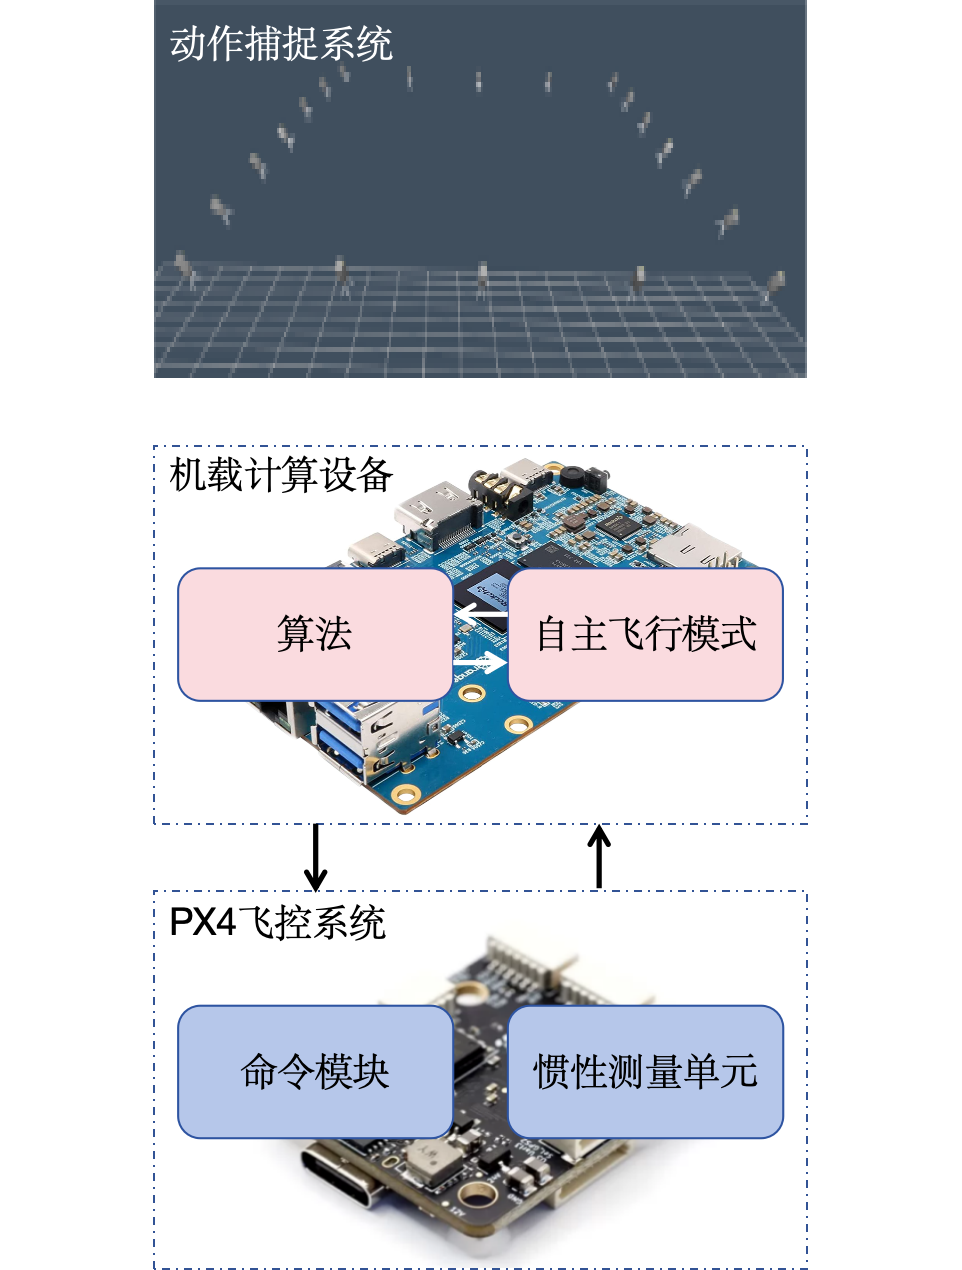
\includegraphics[width=32pc]{picture/图片1.png} 
	\caption{灵敏度传播计算梯度示意图} 
	\label{system}
\end{figure}
此外,灵敏度传播支持在线调整。由于 $\nabla_{\bm{x}_k} T$、$\nabla_{\bm{u}_k} T$、$\nabla_{\bm{x}_k} h$ 和 $\nabla_{\bm{\theta}} h$ 的公式可以离线进行推导,每当系统数据 $\bm{x}_k$ 和 $\bm{u}_k$ 被采样时,灵敏度传播可以在线更新 ${\partial \bm{x}_{k+1}}/{\partial \bm{\theta}}$。此外,预测范围 $N$ 也可以进行在线调整,进一步提高了梯度计算的灵活性。
通过这种方法,可以有效地计算系统参数 $\bm{\theta}$ 对代价函数 $L$ 的灵敏度,进而优化控制策略和系统性能。

\subsection{分布式灵敏度传播方法}
在多无人机系绳吊运系统中,由于无人机与载荷之间的系绳拉力耦合以及无人机之间的间接耦合关系,系统的灵敏度传播变得复杂且计算成本较高。

闭环状态 \( \bm x_{i,k} \) 和 \( \bm x_{l,k} \) 分别通过\autoref{multiuav} 和\autoref{multipayload} 进行迭代定义(即传播)。基于此,灵敏度\( {\partial \bm x_{it}}/{\partial \bm \theta_i} \) 和 \( {\partial \bm x_{lt}}/{\partial \bm \theta_l} \) 可以通过对相应的 MPC 超参数 \( \bm \theta_i \) 和 \( \bm \theta_l \) 求偏导数,分别从两个动态方程的两边进行传播。多无人机绳系吊运系统的灵敏度传播可定义如下:

\begin{equation}
	\begin{gathered}
		\frac{\partial \bm{x}_{i,k+1}}{\partial \bm{\theta}_i} = \bm{F}_{i,k} \frac{\partial \bm{x}_{i,k}}{\partial \bm{\theta}_i} + \bm{F}_{il,k} \frac{\partial \bm{x}_{l,k}}{\partial \bm{\theta}_i} + \bm{G}_{i,k} \bm{U}_{i,k}, \quad \forall i \in \mathcal{I}_q 
		\\
		\frac{\partial \bm{x}_{i,k+1}}{\partial \bm{\theta}_l} = \bm{F}_{l,k} \frac{\partial \bm{x}_{i,k}}{\partial \bm{\theta}_l} + \bm{F}_{li,k} \frac{\partial \bm{x}_{i,k}}{\partial \bm{\theta}_i}, \quad \forall i \in \mathcal{I}_q
		\\
		\frac{\partial \bm{x}_{l,k+1}}{\partial \bm{\theta}_i} = \bm{F}_{i,k} \frac{\partial \bm{x}_{l,k}}{\partial \bm{\theta}_i} + \bm{F}_{il,k} \frac{\partial \bm{x}_{l,k}}{\partial \bm{\theta}_l} + \bm{G}_{il,k} \bm{U}_{l,k}, \quad \forall i \in \mathcal{I}_q
		\\
		\frac{\partial \bm{x}_{l,k+1}}{\partial \bm{\theta}_l} = \bm{F}_{l,k} \frac{\partial \bm{x}_{l,k}}{\partial \bm{\theta}_l} + \sum_{i=1}^{n} \bm{F}_{li,k} \frac{\partial \bm{x}_{i,k}}{\partial \bm{\theta}_l} + \bm{G}_{l,k} \bm{U}_{l,k}
	\end{gathered}
	\label{ss}      
\end{equation}
其中
$$
\bm{F}_{i,k} = \frac{\partial \bar{f}_{i,k}}{\partial \bm{x}_{i,k}} + \frac{\partial \bar{f}_{i,k}}{\partial \bm{u}_{i0}^*} \frac{\partial \bm{u}_{i0}^*}{\partial \bm{x}_{i,k}} + \frac{\partial \bm{u}_{i0}^*}{\partial \bm{u}_{l0}^*} \frac{\partial \bm{u}_{l0}^*}{\partial \bm{x}_{i,k}} + \frac{\partial \bar{f}_{i,k}}{\partial \bm{u}_{l0}^*} \frac{\partial \bm{u}_{l0}^*}{\partial \bm{x}_{i,k}},$$
$$\bm{F}_{il,k} = \frac{\partial \bar{f}_{i,k}}{\partial \bm{x}_{l,k}} + \frac{\partial \bar{f}_{i,k}}{\partial \bm{u}_{i0}^*} \frac{\partial \bm{u}_{i0}^*}{\partial \bm{x}_{l,k}} + \frac{\partial \bm{u}_{i0}^*}{\partial \bm{u}_{l0}^*} \frac{\partial \bm{u}_{l0}^*}{\partial \bm{x}_{l,k}} + \frac{\partial \bar{f}_{i,k}}{\partial \bm{u}_{l0}^*} \frac{\partial \bm{u}_{l0}^*}{\partial \bm{x}_{l,k}},$$
$$\bm{F}_{l,k} = \frac{\partial \bar{f}_{l,k}}{\partial \bm{x}_{l,k}} + \frac{\partial \bar{f}_{l,k}}{\partial \bm{u}_{l0}^*} \frac{\partial \bm{u}_{l0}^*}{\partial \bm{x}_{l,k}}
, \quad \bm{F}_{li,k} = \frac{\partial \bar{f}_{l,k}}{\partial \bm{x}_{i,k}} + \frac{\partial \bar{f}_{l,k}}{\partial \bm{u}_{l0}^*} \frac{\partial \bm{u}_{l0}^*}{\partial \bm{x}_{i,k}},$$
$$\bm{G}_{i,k} = \frac{\partial \bar{f}_{i,k}}{\partial \bm{u}_{i0}^*}
, \quad \bm{G}_{il,k} = \frac{\partial \bar{f}_{i,k}}{\partial \bm{u}_{i0}^*} \frac{\partial \bm{u}_{i0}^*}{\partial \bm{u}_{l0}^*} + \frac{\partial \bar{f}_{i,k}}{\partial \bm{u}_{l0}^*}
, \quad \bm{G}_{l,k} = \frac{\partial \bar{f}_{l,k}}{\partial \bm{u}_{l0}^*},$$
$$\bm{U}_{i,k} = \frac{\partial \bm{u}_{i0}^*}{\partial \bm{\theta}_i}, \quad \bm{U}_{l,k} = \frac{\partial \bm{u}_{l0}^*}{\partial \bm{\theta}_l}$$

\textbf{注4.2:}与单个代理的灵敏度传播相比,式(\ref{ss})额外考虑了每架无人机与载荷之间的动态耦合,这些耦合通过梯度 \( {\partial \bm{u}_{i0}^*}/{\partial \bm{u}_{l0}^*}, {\partial \bm{u}_{i0}^*}/{\partial \bm{x}_{l,k}}, {\partial \bm{u}_{l0}^*}/{\partial \bm{x}_{i,k}}, {\partial \bm{x}_{i,k}}/{\partial \bm{\theta}_l}, {\partial \bm{x}_{l,k}}/{\partial \bm{\theta}_i} \)表示。

对于\autoref{ss} 中的系数矩阵,由于MPC是隐式可微的,其梯度 \( {\partial \bm u_{0}^*}/{\partial \bm x_{}}, {\partial \bm u_{0}^*}/{\partial \bm \theta_{}} \) 无法像简单的反馈控制律 \( \bm u = \bm K \bm x \) 那样直接计算。因此,本节通过构造隐式微分来计算梯度。

对于式 (\ref{multiuav}) 和式 (\ref{multipayload}) 中的非线性 MPC 问题,可以将其表示为以下一般形式:
\begin{equation}
\begin{aligned} 
&\operatorname*{minimize}_{\bm{X}_l, \bm{U}_l} & &  \sum_{k=1}^N{\bm C}_{\bm \theta,k}(\bm x_k,\bm u_k) \\
&\text{subject to} & & \begin{aligned}
& \bm{x}_{k+1} ={f}_{}(\bm{x}_{k}, \bm{u}_{k}) \\
& \bm{x}_{0} = \bm{x}_\text{init}\\
& g(\bm x_k,\bm u_k) \leqslant 0	
\end{aligned}	
\end{aligned}
\label{NMPC}
\end{equation}
其中,非线性成本函数 \( \bm C_{\bm \theta,k} \) 由参数 \( \bm \theta \) 表示,\( f \) 为非线性动态函数,\( g \) 为非线性不等式约束函数。
解决该非线性优化问题的一种常见方法是将其视为非线性规划问题,并应用序列二次规划(SQP),该方法通过迭代生成并优化以下近似问题:
\begin{equation}
\begin{aligned} 
&\operatorname*{minimize}_{\bm{X}_l, \bm{U}_l} & & \frac{1}{2}\bm{\tau}_{t}^{\top}\nabla^{2}\bm C_{\bm \theta,t}^{p}\bm{\tau}_{t}+(\nabla \bm C_{\bm \theta,t}^{p}-\nabla^{2}\bm C_{\bm \theta,t}^{p}\bm{\tau}_{t}^{p})^{\top}\bm{\tau}_{t} \\
&\text{subject to} & & \begin{aligned}
& \bm{x}_{t+1}=\nabla f^{p}\bm{\tau}_{t}+f^{p}-\nabla f^{p}\bm{\tau}_{t}^{p} \\
& \bm{x}_{0} = \bm{x}_\text{init} \\
& \nabla g^{p}\bm{\tau}_{t}\leq\nabla g^{p}\bm{\tau}_{t}^{p}-g^{p}	
\end{aligned}
\end{aligned}	
\label{L-NMPC}
\end{equation}
其中,非线性成本函数和约束在第 \(p\) 次迭代的最优解 \( \{\bm  \tau_t^p \}_{t=1}^{T} \) 处分别进行了泰勒展开,展开至二阶和一阶。所有表示为 \( \nabla \) 的微分是相对于 \( \bm \tau_t \) 进行的,幂次为2表示Hessian矩阵。幂次 \( p \) 表示该函数在第 \( p \) 次迭代得到的最优解处求值。式 (\ref{L-NMPC}) 的解 \( \{\bm \tau_t^{p+1} \}_{t=1}^{T} \) 用于在泰勒展开中构造第 \( p+1 \) 次迭代的SQP。

式 (\ref{L-NMPC}) 的形式与线性MPC的形式完全相同。当SQP在第 \( N \) 次迭代结束时,将 \( \{\bm \tau_t^N \}_{t=1}^{T} \) 作为式 (\ref{NMPC}) 的最优解,根据文献\oldcite{tao2024difftune}中的定理1,使用线性MPC方法计算梯度。通过链式法则,可以得到目标梯度 \( {\partial \bm u_0^\star}/{\partial \bm \theta} \) 和 \( {\partial \bm u_0^\star}/{\partial \bm x_{\text{init}}} \),用于迭代更新学习参数。

由\textbf{注4.2}可知,系绳引起的强动力学耦合作用使得每个智能体的闭环状态不仅受到自身控制器的影响,还会受到其他智能体控制器的影响。因此,灵敏度状态还需要考虑无人机闭环状态相对于载荷MPC超参数的梯度和载荷闭环状态相对于无人机MPC超参数的梯度${\partial \bm{x}_{i,k}}/{\partial \bm{\theta}_l}$和${\partial \bm{x}_{l,k}}/{\partial \bm{\theta}_i}$。

在求解上述两个梯度时,借助第3章中提出的 Neural Predictor 方法。由式(\ref{nmpc})中的动力学模型可知,在无人机系统中,无人机的动力学和载荷的动力学可以分为两类,分别是无人机动力学和学习得到的载荷动力学。Neural Predictor可以用于预测系绳连接的载荷动力学。
对于每架无人机,可以将学习得到的载荷动力学模型与无人机自身的动力学模型相结合,载荷闭环状态相对于无人机MPC超参数的梯度可以通过学习得到的动力学模型进行显式计算。而对于无人机闭环状态相对于载荷MPC超参数的梯度,情况有所不同。由于载荷上的虚拟控制输入 \( \bm{u}_l = \left[ \bar{T}_1, \cdots, \bar{T}_n \right] \) 实际上可以在Neural Predictor中用无人机的状态 \( \bm{x}_i \) 进行预测,因此无人机闭环状态相对于载荷MPC超参数的梯度可以直接通过载荷闭环状态相对于载荷MPC超参数的梯度进行体现。最终,通过这一系统化的求解过程,可以实现灵敏度的分布式并行传播。具体的算法流程总结如算法 \ref{alg:sensitivity_propagation} 所示。
\begin{algorithm}[H]
	\captionsetup{font={stretch=1.2}}
	\linespread{1.2}\selectfont % 设置行距为1.2倍
	\caption{分布式灵敏度传播算法}
	\label{alg:sensitivity_propagation}
	\textbf{输入:} 目标梯度动力学系统的系数矩阵,新的控制输入 $\{\bm{U}_t\}_{k=T}^{T+N_{\text{}}}$,初始条件 ${\frac{\partial \bm{x}_{T}}{\partial \bm{\theta}}} = 0$。\\
	\textbf{输出:} 灵敏度轨迹 ${\frac{\partial \bm{x}_{k}}{\partial \bm{\theta}}}, (\forall k = T, \cdots, T+N_{\text{}})$。
	
	\begin{algorithmic}[1]
		\For{$i = 1$ \textbf{to} $n$ ($in$ $parallel$)}
		\For{$k = T$ \textbf{to} $T+N_{\text{}}$}
		\State 从“中央无人机”接收载荷灵敏度 $\frac{\partial \bm{x}_{l,k}}{\partial \bm{\theta}_l}$
		\State 基于接收到的 $\frac{\partial \bm{x}_{l,k}}{\partial \bm{\theta}_l}$ 使用\autoref{ss}计算灵敏度 $\frac{\partial \bm{x}_{i,k}}{\partial \bm{\theta}_i}, \frac{\partial \bm{x}_{l,k}}{\partial \bm{\theta}_i}, \frac{\partial \bm{x}_{i,k}}{\partial \bm{\theta}_l}$
		\State 将 $\frac{\partial \bm{x}_{i,k}}{\partial \bm{\theta}_l}$ 发送至“中央无人机”
		\EndFor
		\EndFor
		
		\For{$k = T$ \textbf{to} $T+N_{\text{}}$}
		\Statex $\triangleright$ 在“中央无人机”中
		\State 接收来自所有无人机的灵敏度 $\frac{\partial \bm{x}_{i,k}}{\partial \bm{\theta}_l}, \forall i \in \mathcal{I}_q$
		\State 使用\autoref{ss}基于接收到的 $\frac{\partial \bm{x}_{l,k}}{\partial \bm{\theta}_l}, \forall i \in \mathcal{I}_q$ 计算载荷的灵敏度轨迹 $\frac{\partial \bm{x}_{l,k}}{\partial \bm{\theta}_l}$
		\EndFor
	\end{algorithmic}
\end{algorithm}

\subsection{分布式策略梯度算法}
对于多无人机绳系吊运系统,其动态行为复杂,难以通过解析模型精确描述。因此,引入深度神经网络(DNN)生成控制器的动态权重和参考轨迹,DNN 的输入特征包括系统状态、障碍物位置等环境信息。第 \(i\) 个无人机的自适应模型预测控制超参数和载荷的自适应模型预测控制超参数可以表示为:

\begin{equation}
	\label{4}
	\begin{gathered}
		\boldsymbol{\theta}_i=h_{\boldsymbol{\pi}_i}\left(\boldsymbol{\chi}_i\right),\mathrm{~}\forall i\in\mathcal{I}_q\\    
		\boldsymbol{\theta}_l=h_{\boldsymbol{\pi}_l}\left(\boldsymbol{\chi}_l\right)
	\end{gathered}
\end{equation}
其中,\( \bm \pi_i \) 表示第 \(i\) 个无人机的DNN的可学习参数,\( \bm \pi_l \) 表示载荷的DNN的可学习参数,\( \bm \chi_i \) 和\( \bm \chi_l \) 分别包含无人机和载荷的环境观测数据及系统相关信息,例如系统状态和障碍物信息等。为了确保MPC超参数 \( \bm \theta_i \) 在物理上合理且计算上受限,采用以下参数化形式:
\begin{equation}
    \bm \theta_i = \bm \theta_{i,\text{min}} + \left( \bm \theta_{i,\text{max}} - \bm \theta_{i,\text{min}} \right) \bm \Theta_i, \quad \forall i \in \mathcal{I}_A,
\end{equation}
其中,\( \bm \theta_{i,\text{min}} \) 和 \( \bm \theta_{i,\text{max}} \) 分别表示超参数的下限和上限,\( \bm \Theta_i \) 为归一化超参数,范围在 \([\text{0}, \text{1}]\) 之间。

通过优化每个无人机和载荷的DNN参数 \( \pi_i^* \)和\(\bm \pi_l\),最小化由所有无人机的代价函数构成的总体代价函数,进而实现自适应控制。该问题可以用以下优化问题表示:

\begin{equation}
	\begin{aligned} 
		&\operatorname*{minimize}_{\bm{\pi}} & & L_l+\sum_{i=1}^{n}L_i \\
		&\text{subject to} & & \begin{aligned}
			&\boldsymbol{x}_{i,{k+1}} = {{f}}_{i,k}\left(\boldsymbol{x}_{i,k}, \boldsymbol{u}^*_{i,{k}},  \boldsymbol{x}_{l,k}, \boldsymbol{u}^*_{l,{k}}\right), \forall i \in \mathcal{I}_q \\
			&\boldsymbol{x}_{l,{k+1}} = {{f}}_{l,k}\left(\boldsymbol{x}_{l,k}, \boldsymbol{u}^*_{{l},{k}},  \boldsymbol{x}_{i,k}\right), \forall i \in \mathcal{I}_q
		\end{aligned} \\
	\end{aligned}
\end{equation}
其中,$L_l $和 $L_i$分别表示载荷和第 \(i\) 个无人机的代价函数,损失基于它们在给定预测时间范围 \( N \in \mathbb{R}^+ \) 内的状态变化计算。参数 \(\bm \pi \) 包含了所有无人机的DNN参数 \( \bm \pi_i \)和载荷的DNN参数 \( \bm \pi_l \),
第 \(i\) 个无人机的模型预测控制器在超参数\( \boldsymbol{\theta}_i \)下于时刻 \(k\) 生成的最优控制输入记为 \( \boldsymbol{u}^*_{i,{k}} \) ,载荷的模型预测控制器在超参数\( \boldsymbol{\theta}_l \)下于时刻 \(k\) 生成的最优控制输入记为\( \boldsymbol{u}^*_{l,{k}} \)。


% 在本节中,提出了一种分布式策略梯度学习算法,结合分布式灵敏度传播,用于实现自动多机提升系统(Auto-Multilift)。该算法使深度神经网络(DNN)参数 $\bm \pi$ 能够在分布式闭环环境中高效训练。
本小节中,提出了一种分布式策略梯度学习算法,结合分布式灵敏度传播,用于通过梯度下降法学习 DNN 参数 $\bm \pi$:
\begin{equation}
    \bm \pi\leftarrow \bm \pi-\alpha\nabla_{\bm \pi}L
	\label{6}
\end{equation}

多无人机绳系吊运系统中存在的耦合效应,在闭环训练中,无人机 DNN 参数的梯度\( \bm{\nabla}_ {\bm \pi_i}  L \) 和载荷 DNN 参数的梯度 \( \bm{\nabla}_ {\bm \pi_l}  L \)可分别使用链式法则表达为:
\begin{equation}
	\begin{gathered}
		\bm{\nabla}_ {\bm \pi_i}  L = \left(\sum_{k=1}^{N} \frac{\partial L_i}{\partial \bm x_{i,k}} \frac{\partial \bm x_{i,k}}{\partial \bm \theta_i} + \sum_{k=1}^{N} \frac{\partial L_l}{\partial \bm x_{l,k}} \frac{\partial \bm x_{l,k}}{\partial \bm \theta_i} +\sum_{k=0}^{N-1} \frac{\partial L}{\partial \bm u_{i,k}} \frac{\partial \bm u_{i,k}}{\partial \bm \theta_i}\right)\frac{\partial\boldsymbol{\theta}_{i}}{\partial\boldsymbol{\Theta}_{i}}\frac{\partial\boldsymbol{\Theta}_{i}}{\partial\boldsymbol{\pi}_{i}},\forall i\in\mathcal{I}_q\\
		\bm{\nabla}_ {\bm \pi_l} L = \left(\sum_{k=1}^{N} \frac{\partial L_l}{\partial \bm x_{l,k}} \frac{\partial \bm x_{l,k}}{\partial \bm \theta_l} +\sum_{i=1}^{N} \sum_{k=1}^{N} \frac{\partial L_i}{\partial \bm x_{i,k}} \frac{\partial \bm x_{i,k}}{\partial \bm \theta_l} + \sum_{k=0}^{N-1} \frac{\partial L}{\partial \bm u_{l,k}} \frac{\partial \bm u_{l,k}}{\partial \bm \theta}\right)\frac{\partial\boldsymbol{\theta}_{l}}{\partial\boldsymbol{\Theta}_{l}}\frac{\partial\boldsymbol{\Theta}_{l}}{\partial\boldsymbol{\pi}_{l}}
	\end{gathered}
    % \bm{\nabla_\pi L} = \sum_{k=1}^{N} \frac{\partial L}{\partial \bm x_{i,k}} \frac{\partial \bm x_k}{\partial \bm \theta} + \sum_{k=0}^{N} \frac{\partial L}{\partial \bm u_k} \frac{\partial \bm u_k}{\partial \bm \theta}
	\label{7}
\end{equation}
其中,${\partial L}/{\partial \bm x_{i,k}} , {\partial L}/{\partial \bm x_{l,k}} , {\partial L}/{\partial \bm u_k} , {\boldsymbol{\theta}_i}/{\partial\boldsymbol{\pi}_i} , {\boldsymbol{\theta}_l}/{\partial\boldsymbol{\pi}_l}$这些参数都可以通过显函数微分直接确定,无人机闭环状态相对于载荷MPC超参数的梯度\({\partial \bm x_{i,k}}/ {\partial \bm \theta_l}\)和载荷闭环状态相对于无人机MPC超参数的梯度\({\partial \bm x_{l,k}}/{\partial \bm \theta_i}\)则可以通过算法 \ref{alg:sensitivity_propagation} 进行灵敏度传播计算灵敏度状态。


\begin{figure}[H]
	\centering
	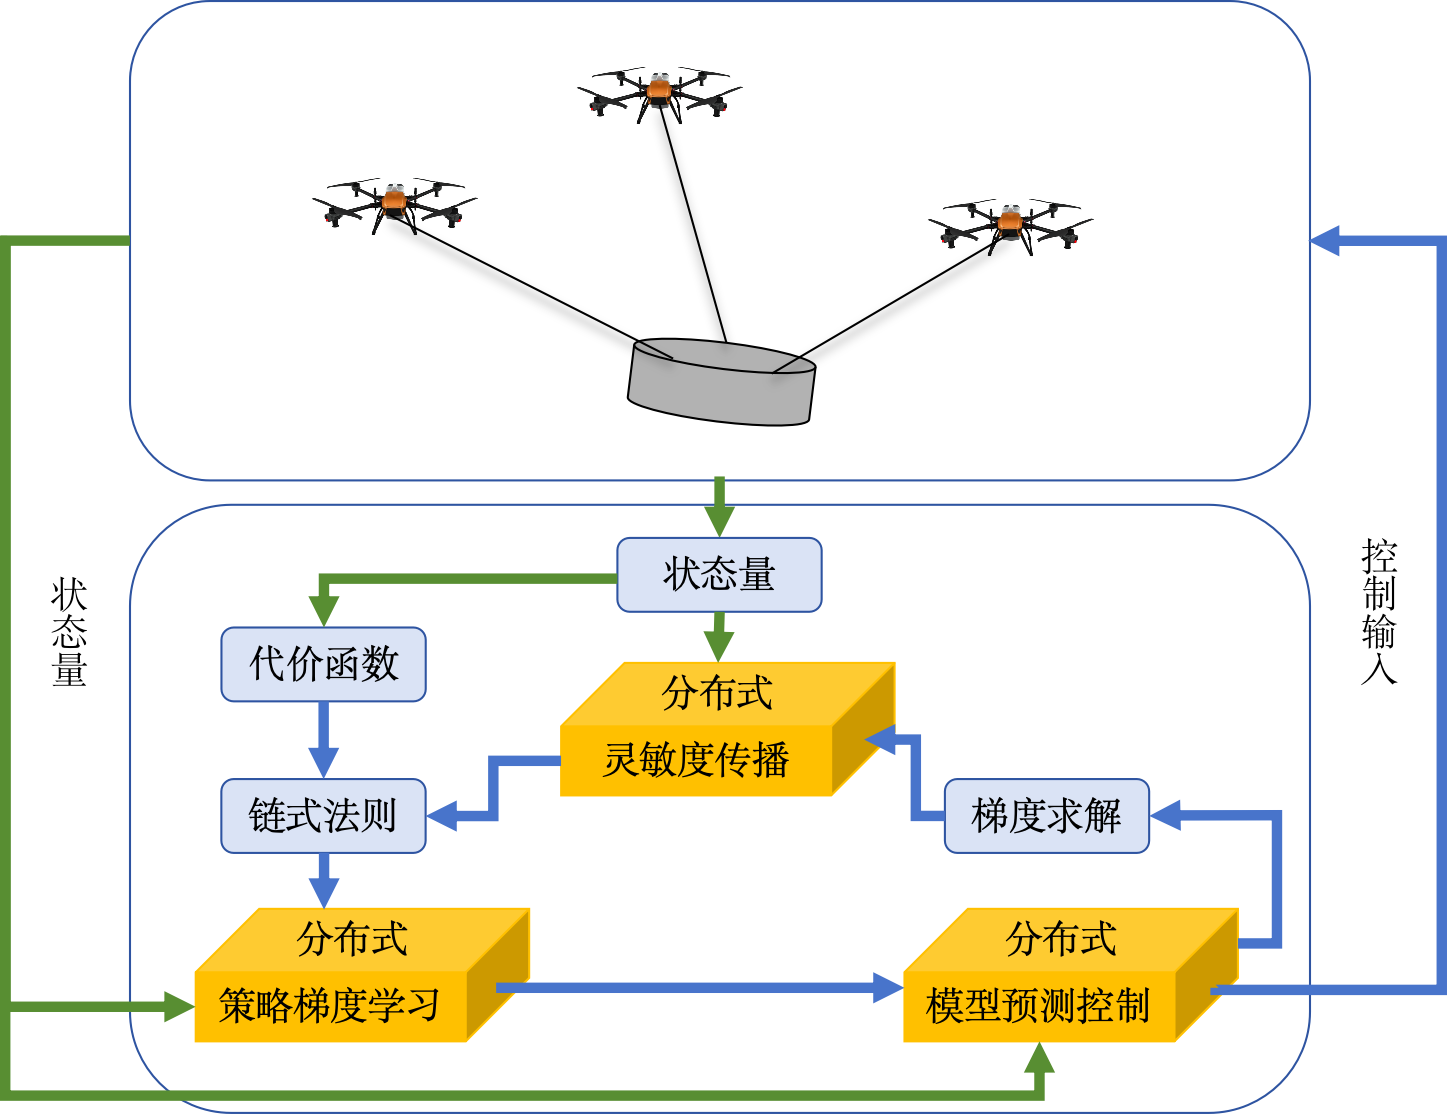
\includegraphics[width=34pc]{picture/4_1.png} 
	\caption{多无人机系统数据驱动控制算法整体框架} 
	\label{4_1}
\end{figure}
\autoref{4_1} 显示了该算法的整体流程,包含前向分布式 MPC 求解与后向策略梯度训练。训练过程总结如算法 \ref{alg:distributed_pg} 所示,其中 $L_{\text{mean}}$ 为一个训练周期(持续时间为 $T_{\text{ep}}$)内各个体损失之和的平均值,$\Delta \bar{t}$ 为离散化实际系统动力学所用的时间步长。
通过这种方法,分布式策略梯度算法能够有效地训练多无人机绳系吊运系统中的 DNN 参数,实现如轨迹跟踪和避障等功能的优化。
\begin{algorithm}[H]
	\captionsetup{font={stretch=1.2}}
	\linespread{1.2}\selectfont % 设置行距为1.2倍
	\caption{分布式策略梯度}
	\label{alg:distributed_pg}
	\textbf{输入:} 学习率 $\epsilon$ 和预先规划的参考轨迹 $x_{i,{\text{ref}}}, \, \forall i \in \mathcal{I}_A$\\
	\textbf{初始化:} $\pi_0$
	
	\begin{algorithmic}[1]
		\While{$L_{\text{mean}}$ $not$ $converged$}
		\For{$k = 0$ \textbf{to} $T_{\text{ep}}$ \textbf{by} $\Delta \bar t$ }
		\State \textbf{前向传播:}
		\State 使用\autoref{4}计算自适应超参数 $\bm{\theta}_{i,k}, \, \forall i \in \mathcal{I}_A$;
		\State 使用\autoref{alg:mpc_multilift}计算 $\bm{u}_{i,k}^{\ast}, \, \forall i \in \mathcal{I}_A$;
		\State 计算每个无人机和载荷的损失函数 $L_{i,k}, \, \forall i \in \mathcal{I}_A$;
		
		\For{$i = 1$ \textbf{to} $n$}
		\State 使用 Neural Predictor 计算 $T_{i,k}$;
		\State 将 $\bm{u}_{i,k}^{\ast}$ 和 $-T_{i,k}$ 应用于无人机数学模型 (\ref{eq:混合模型}),以更新无人机闭环状态 $x_{i,k}$;
		\EndFor
		
		\State 将 $\left\{ T_{i,k} \right\}_{i=1}^n$ 应用于载荷数学模型 (\ref{2-15}),以更新无人机闭环状态 $x_{l,k}$;
		
		\State \textbf{反向传播:}
		\For{$i = 1$ \textbf{to} $n$}
		\State 使用算法 \ref{alg:sensitivity_propagation} 计算无人机的 MPC 相关梯度 $\frac{\partial \bm{x}_{l,k}}{\partial \bm{\theta}_i}$;
		\State 使用算法 \ref{alg:sensitivity_propagation} 计算载荷的 MPC 相关梯度 $\frac{\partial \bm{x}_{i,k}}{\partial \bm{\theta}_l}$;
		\EndFor
		
		\If{$k \geq N$}
		\State 通过 $T_{\text{}} \gets k - N$ 确定起始步;
		\State 计算系统矩阵;
		\State 使用式(\ref{7})计算 $\bm{\nabla}_{\bm{\pi}_i} L, \, \forall i \in \mathcal{I}_A$;
		\State 使用基于梯度的优化方法\autoref{6}更新 $\bm{\pi}_k$;
		\Else
		\State 保持 $\bm{\pi}_k$ 不变;
		\EndIf
		\EndFor
		\State 计算 $L_{\text{mean}} = \frac{\Delta t}{T_{\text{ep}}} \sum_{i=1}^n \sum_{k=0}^{T_{\text{ep}}} L_{i,k}$,作为下一次迭代的训练误差;
		\EndWhile
	\end{algorithmic}
\end{algorithm}

\section{仿真验证}
在本节中,通过数值仿真验证了Autotune在飞行场景下学习各种 MPC 超参数的性能。 采用多层感知机(MLP)网络在线生成自适应归一化超参数。 网络的输出层使用Sigmoid激活函数,将输出限制在0到1之间。\autoref{network}展示了网络的完整架构,其中包含两个使用ReLU激活函数的隐藏层。 为增强网络的鲁棒性和泛化能力,线性层采用谱归一化方法,通过限制层的Lipschitz常数来实现。 为了减少网络规模,将系统中的MPC权重矩阵限制为对角矩阵,使其中每个无人机有28个权重,载荷有24+n个权重。 隐藏层的神经元数量设定为30,输入为无人机和载荷的跟踪误差,自适应MPC权重的上下限分别设定为0.01和100。

\begin{figure}[hbt!]
	\centering
	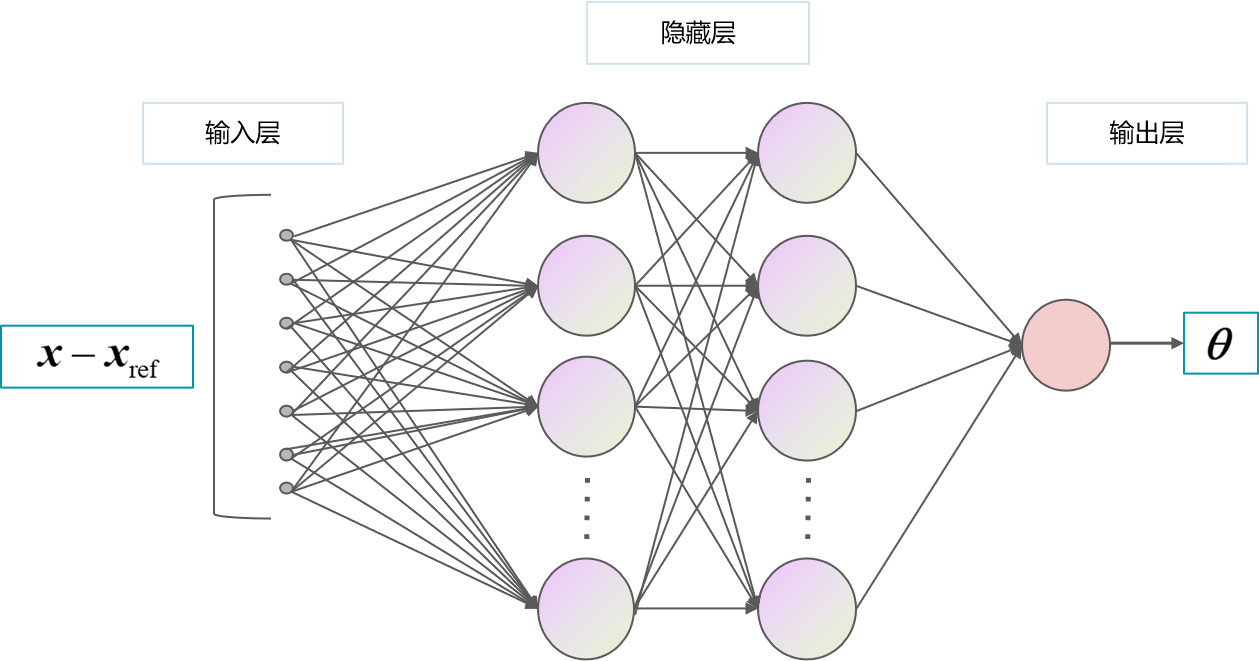
\includegraphics[width=30pc]{picture/kk/图片3.png} 
	\caption{在线自适应 MPC 超参数 $\bm \theta$ 的神经网络架构} 
	\label{network}
\end{figure}
仿真中考虑了一个具有非均匀载荷质量分布的多无人机绳系吊运系统,由3架0.75 kg的无人机吊运1.5 kg载荷,其中载荷的质心坐标的偏差值设定为 $\bm p_{l}^g=[\text{0.1},\text{0.1},\text{-0.1}]$ m。在这种情况下,无人机之间需要在飞行过程中进行动态的拉力分配才能保持载荷的平衡,因此需要自适应选择 MPC 权重。在这种情况下,需要对三架无人机和载荷上的自适应网络同时进行并行闭环训练。在训练中将MPC预测范围设为10,闭环训练的损失范围设为20。分布式MPC问题\autoref{multiuav} 和\autoref{multipayload} 使用\autoref{alg:mpc_multilift} 中的方法以滚动时域方式求解。
每个训练周期包括在每个无人机和载荷上的10秒参考轨迹上并行训练这些网络一次(即\autoref{alg:distributed_pg}中的$T_{ep}= \text{10s}$)。

\begin{figure}[hbt!]
	\centering
	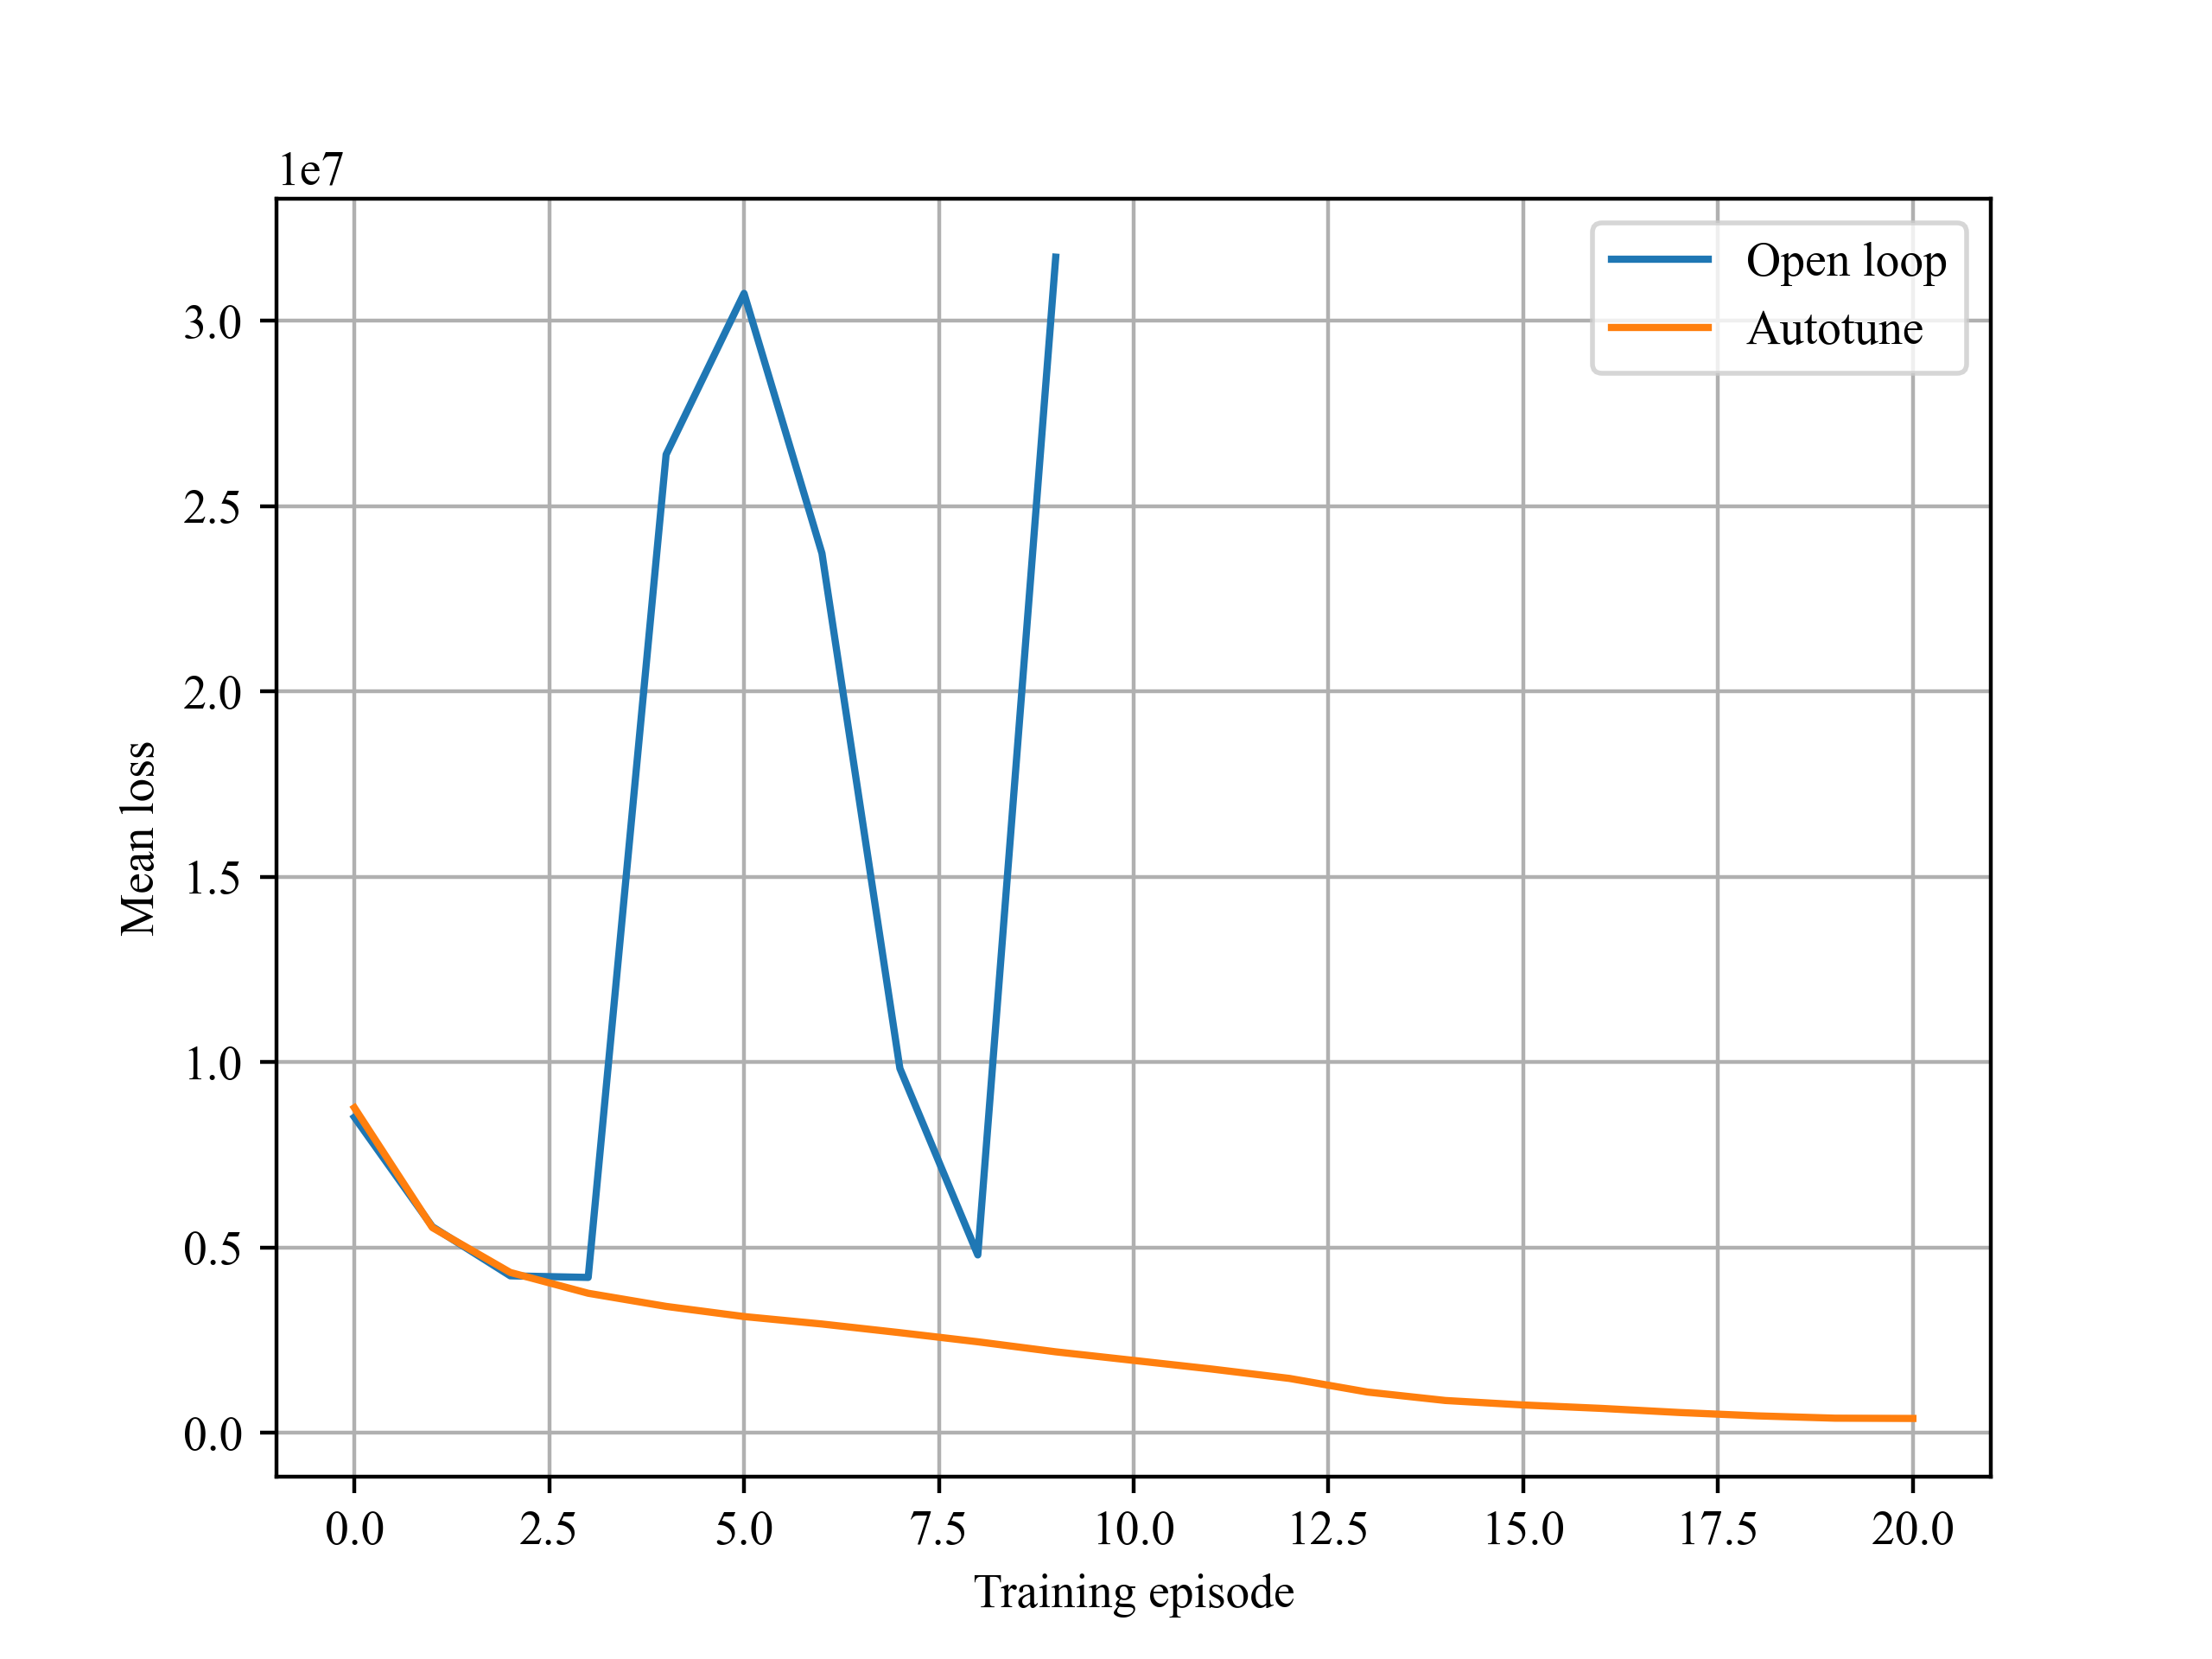
\includegraphics[width=30pc]{picture/kk/Mean_loss_cln.png} 
	\caption{开环训练算法和分布式策略梯度训练算法的平均损失对比} 
	\label{meanloss}
\end{figure}

\begin{figure}[hbt!]
	\centering
	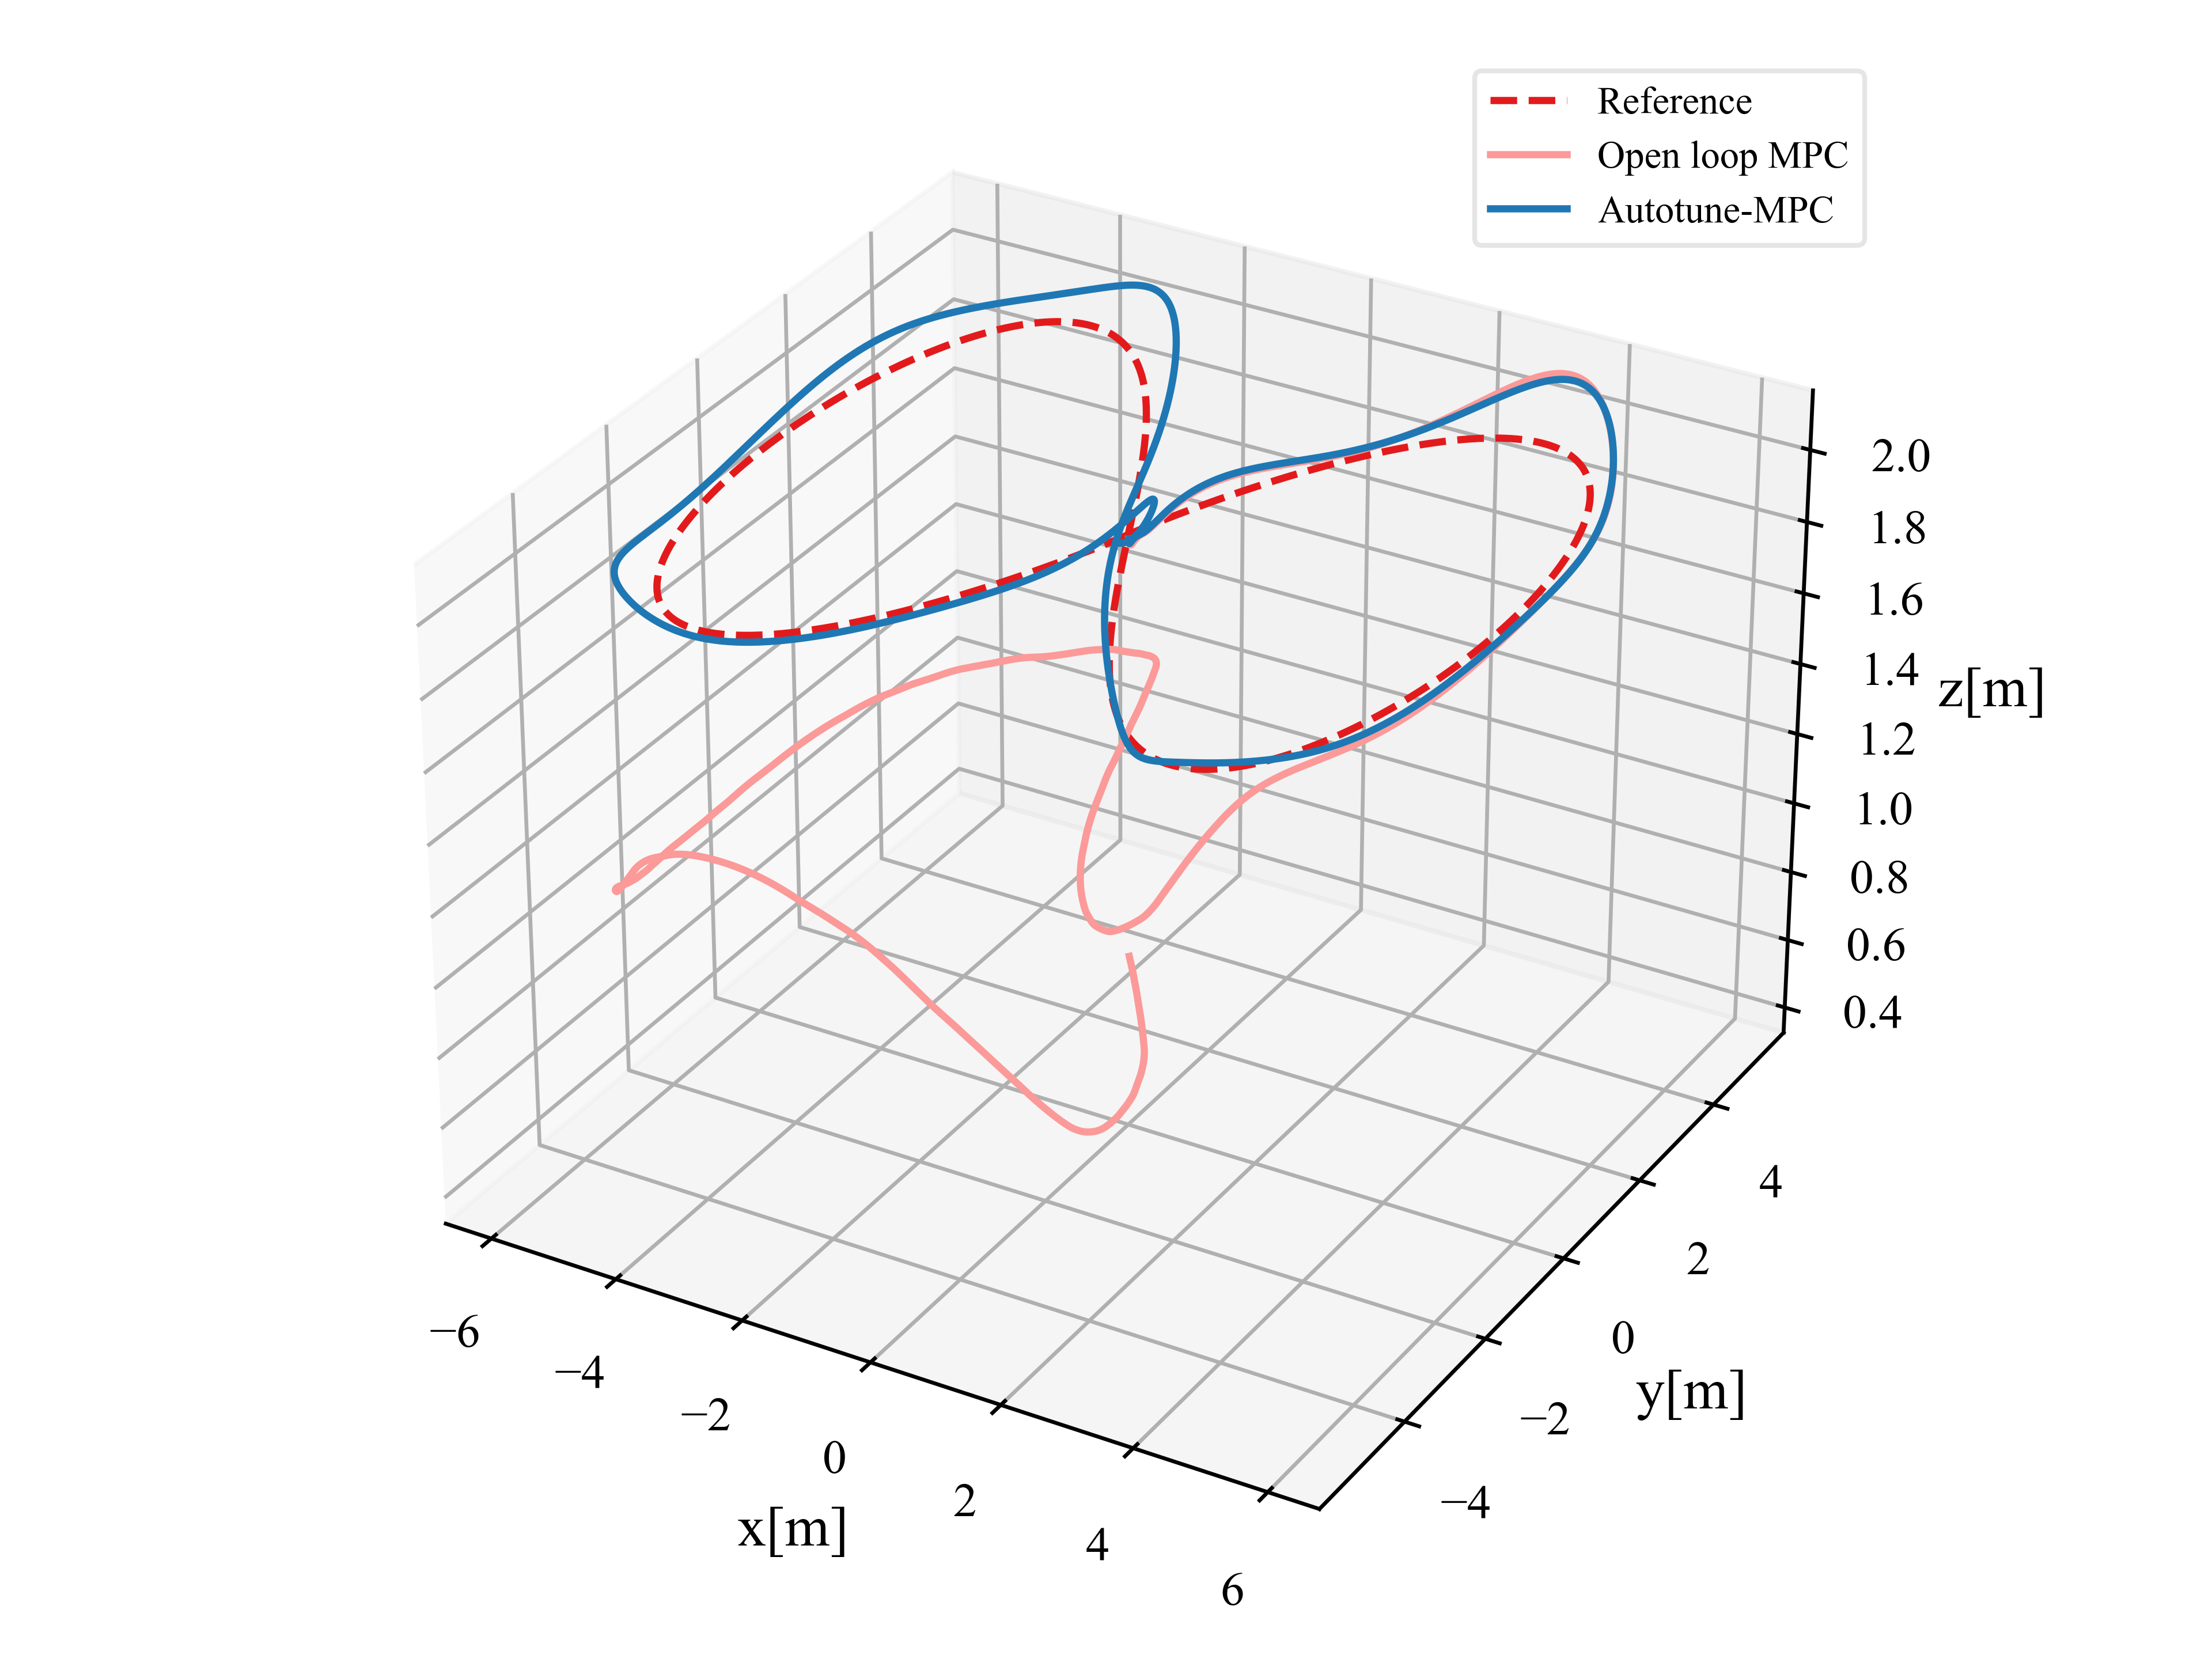
\includegraphics[width=36pc]{picture/kk/plot3D.png} 
	\caption{开环训练算法与分布式策略梯度训练算法在轨迹跟踪中的3D对比图} 
	\label{cjb}
\end{figure}

\autoref{meanloss} 比较了Autotune与开环训练方法在多无人机绳系吊运系统的平均损失。为了公平比较,图中显示的所有平均损失均使用相同的损失函数。对于具有较重载荷的多无人机绳系吊运系统,开环训练方法没有考虑系统中的强耦合项,导致训练不稳定,平均损失呈发散趋势。相比之下,Autotune的平均损失均能稳定在更小的值,体现了稳定学习和更佳跟踪性能的优势。

\autoref{cjb} 以3D图的方式展示了训练过程。Autotune在训练周期中提高了跟踪性能,同时逐渐将载荷的姿态稳定在期望的水平位置。相较于开环训练的MPC方法,Autotune-MPC的优势主要源于直接在实际系统动力学的闭环系统状态上进行训练,而前者依赖于名义动力学中预测得到的开环状态。如\autoref{cjb1} 所示,MPC计算的拉力比实际拉力平滑得多,在Autotune-MPC中,使用MPC计算的得到的拉力代替实际拉力,解决了实际拉力和MPC计算拉力之间的差异。
尽管这两种方法都通过对MPC进行自适应调参以提高鲁棒性,但基于闭环数据进行训练的Autotune-MPC方法提供了一种更加稳健和高效的途径来提升跟踪性能。在16
秒左右,系绳上的实际拉力存在高频波动,Autotune-MPC能够有效计算出适当的梯度来稳定训练,而开环训练方法则导致了不稳定。
% \begin{figure}[hbt!]
% 	\centering
% 	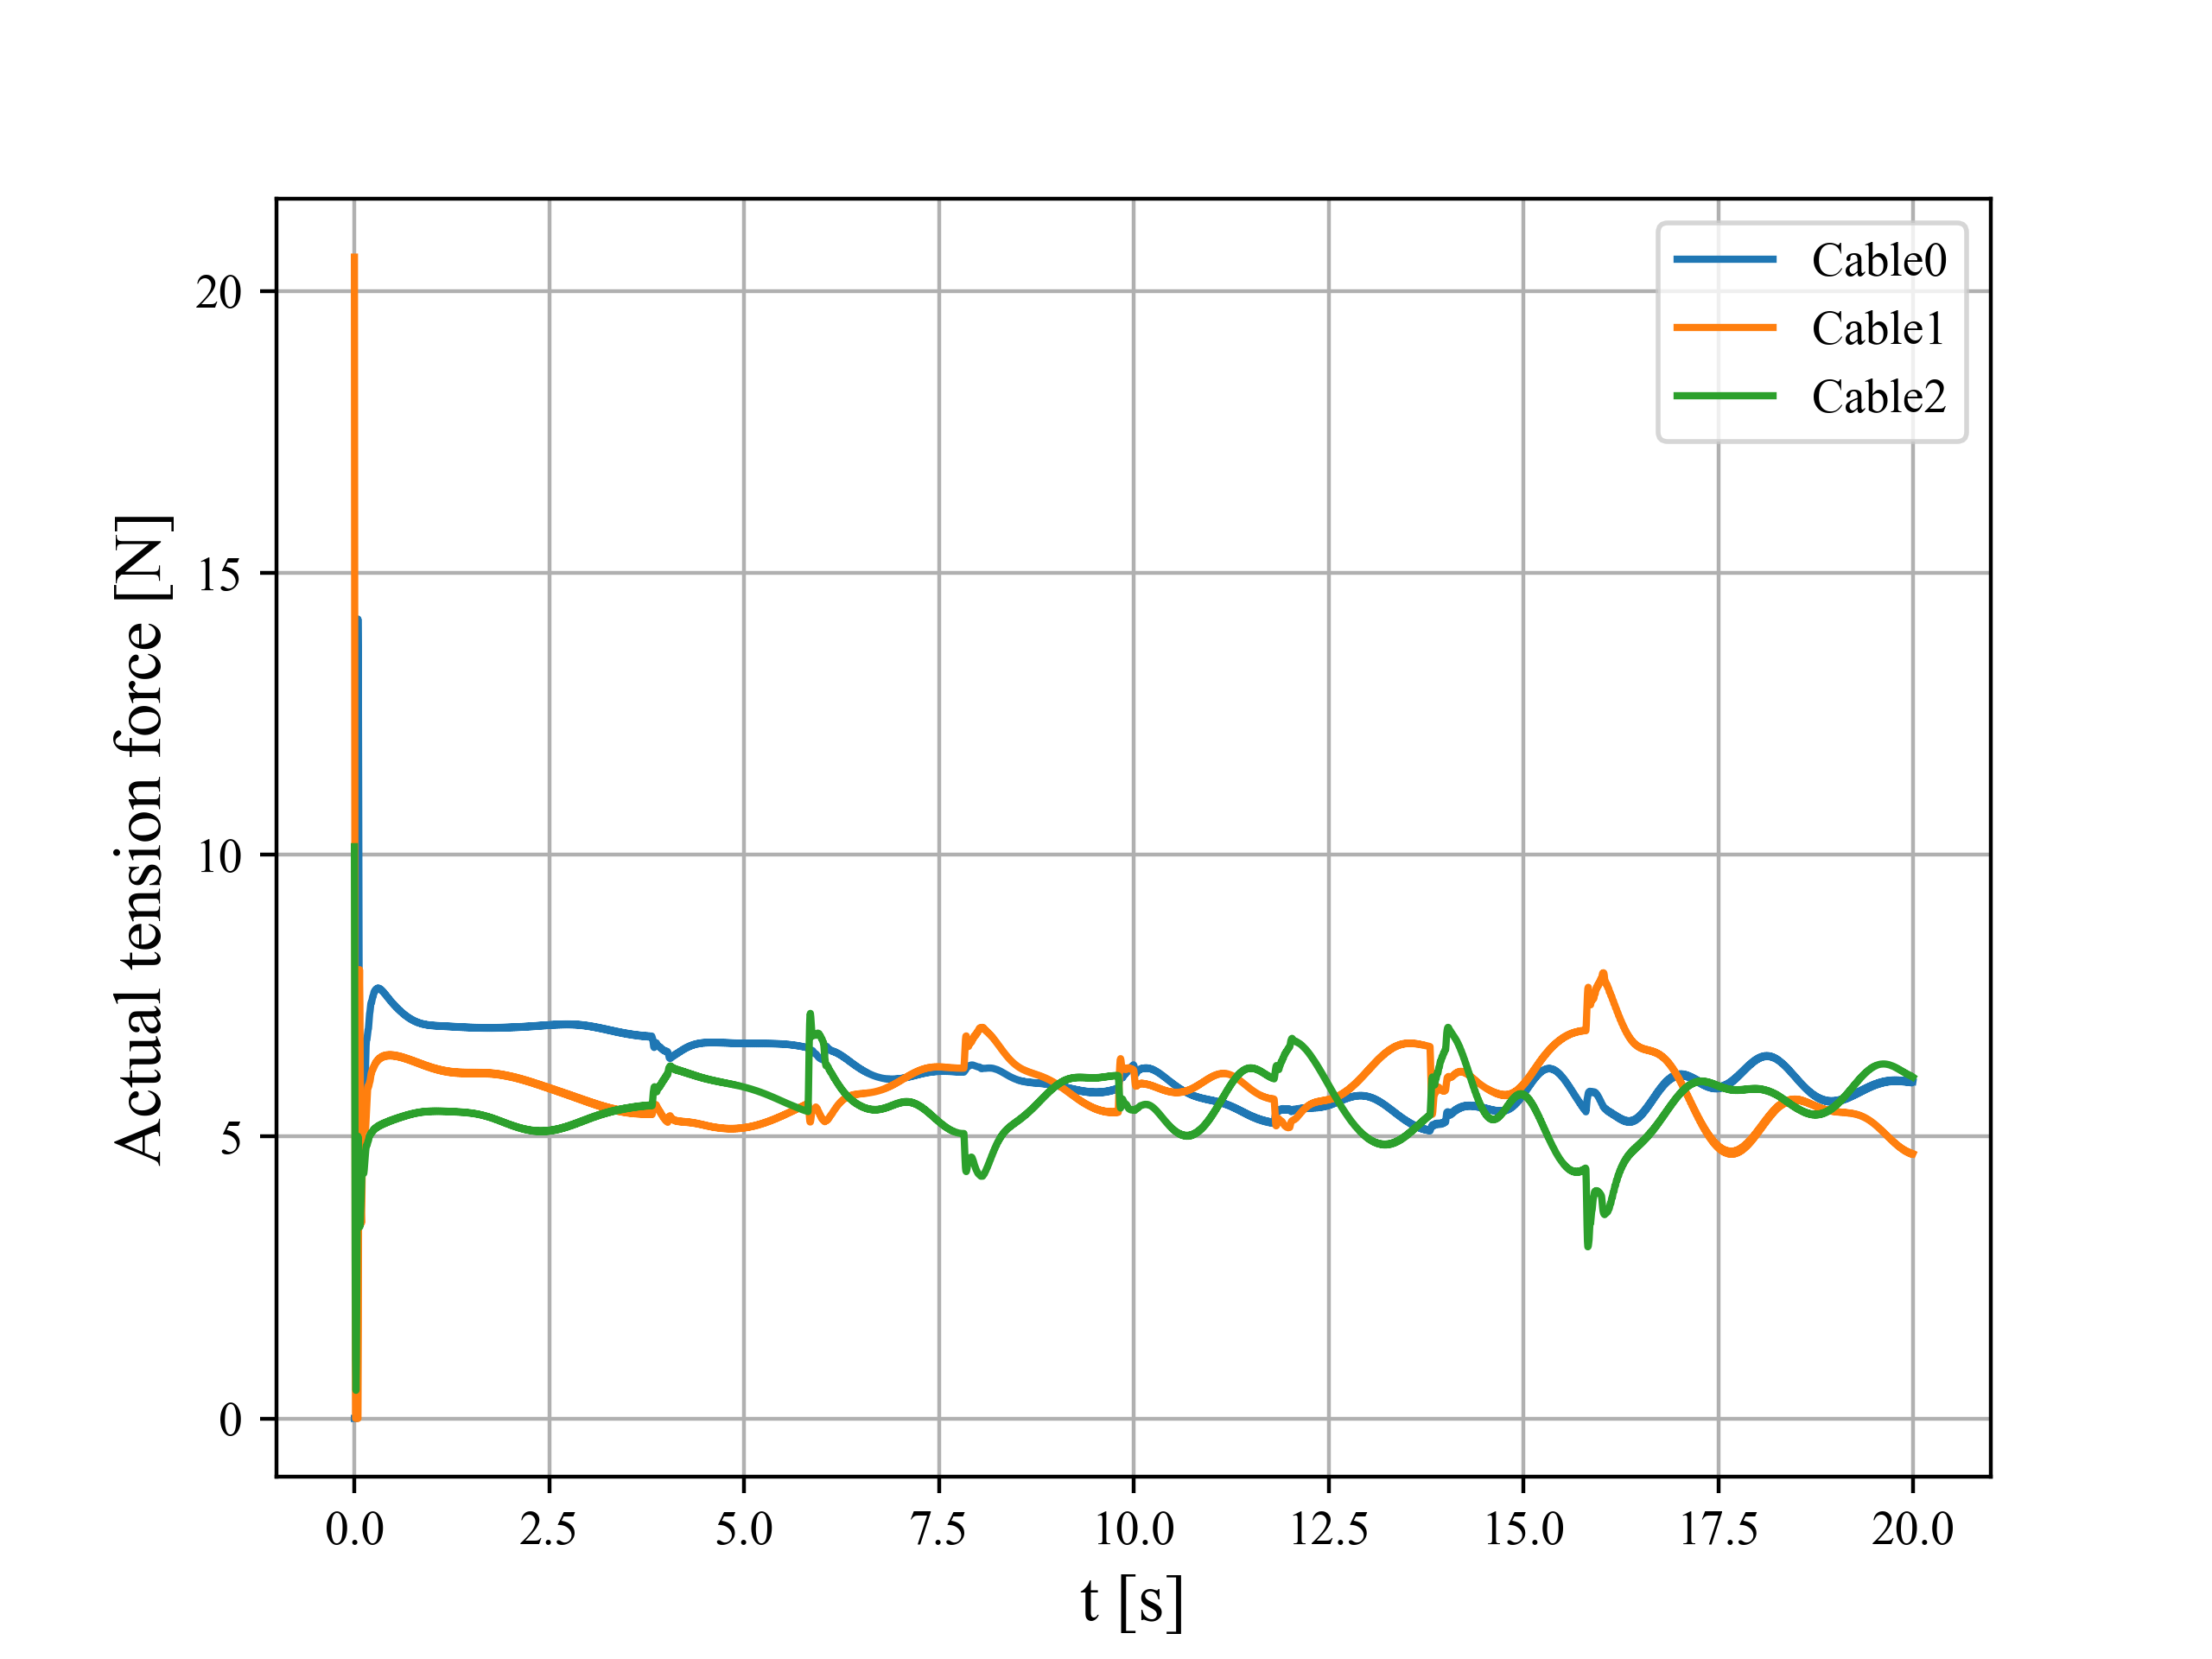
\includegraphics[width=32pc]{picture/kk/cable_actual_tensions_fig_8_6quad_ol.png} 
% 	\caption{闭环训练过程中系绳上的实际拉力大小} 
% 	\label{cjb1}
% \end{figure}


% \begin{figure}[hbt!]
% 	\centering
% 	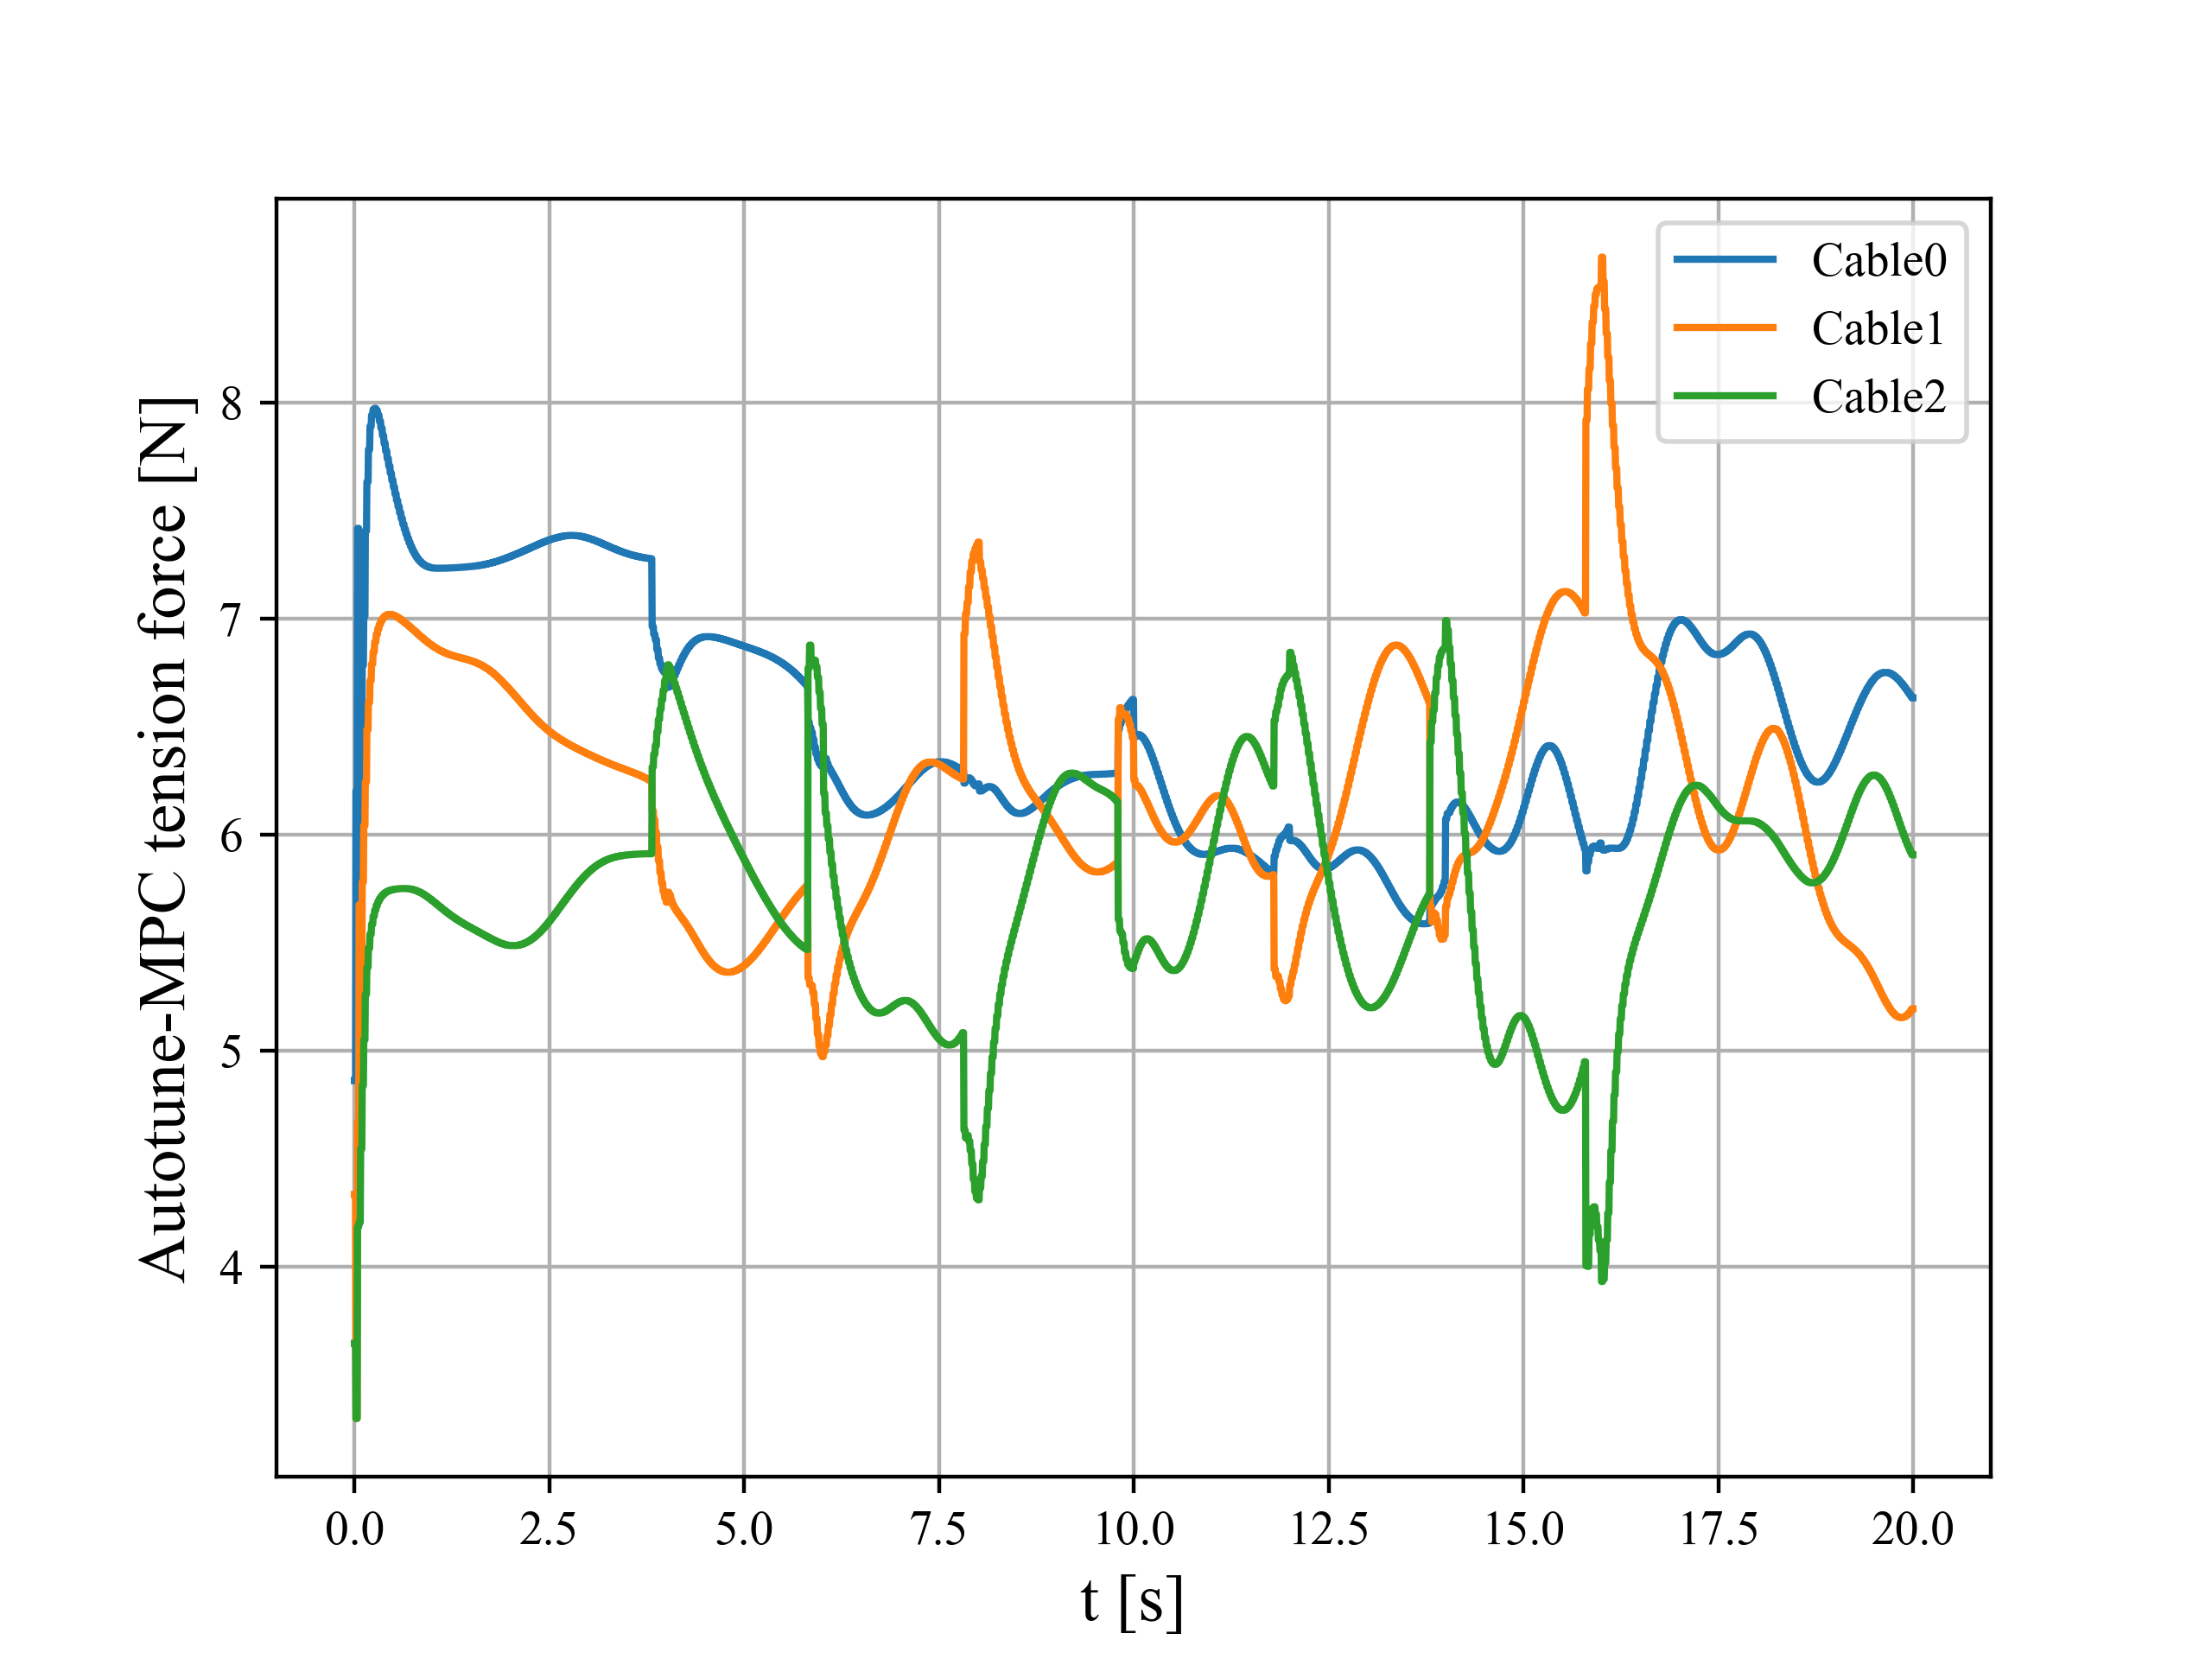
\includegraphics[width=32pc]{picture/kk/cable_MPC_tensions_fig_8_6quad_ol.png} 
% 	\caption{闭环训练过程中系绳上的MPC计算拉力大小} 
% 	\label{cjb2}
% \end{figure}
\begin{figure}[hbt!]
    \centering
    % 第一行的两张图
    \begin{subfigure}[b]{0.48\textwidth}
        \centering
        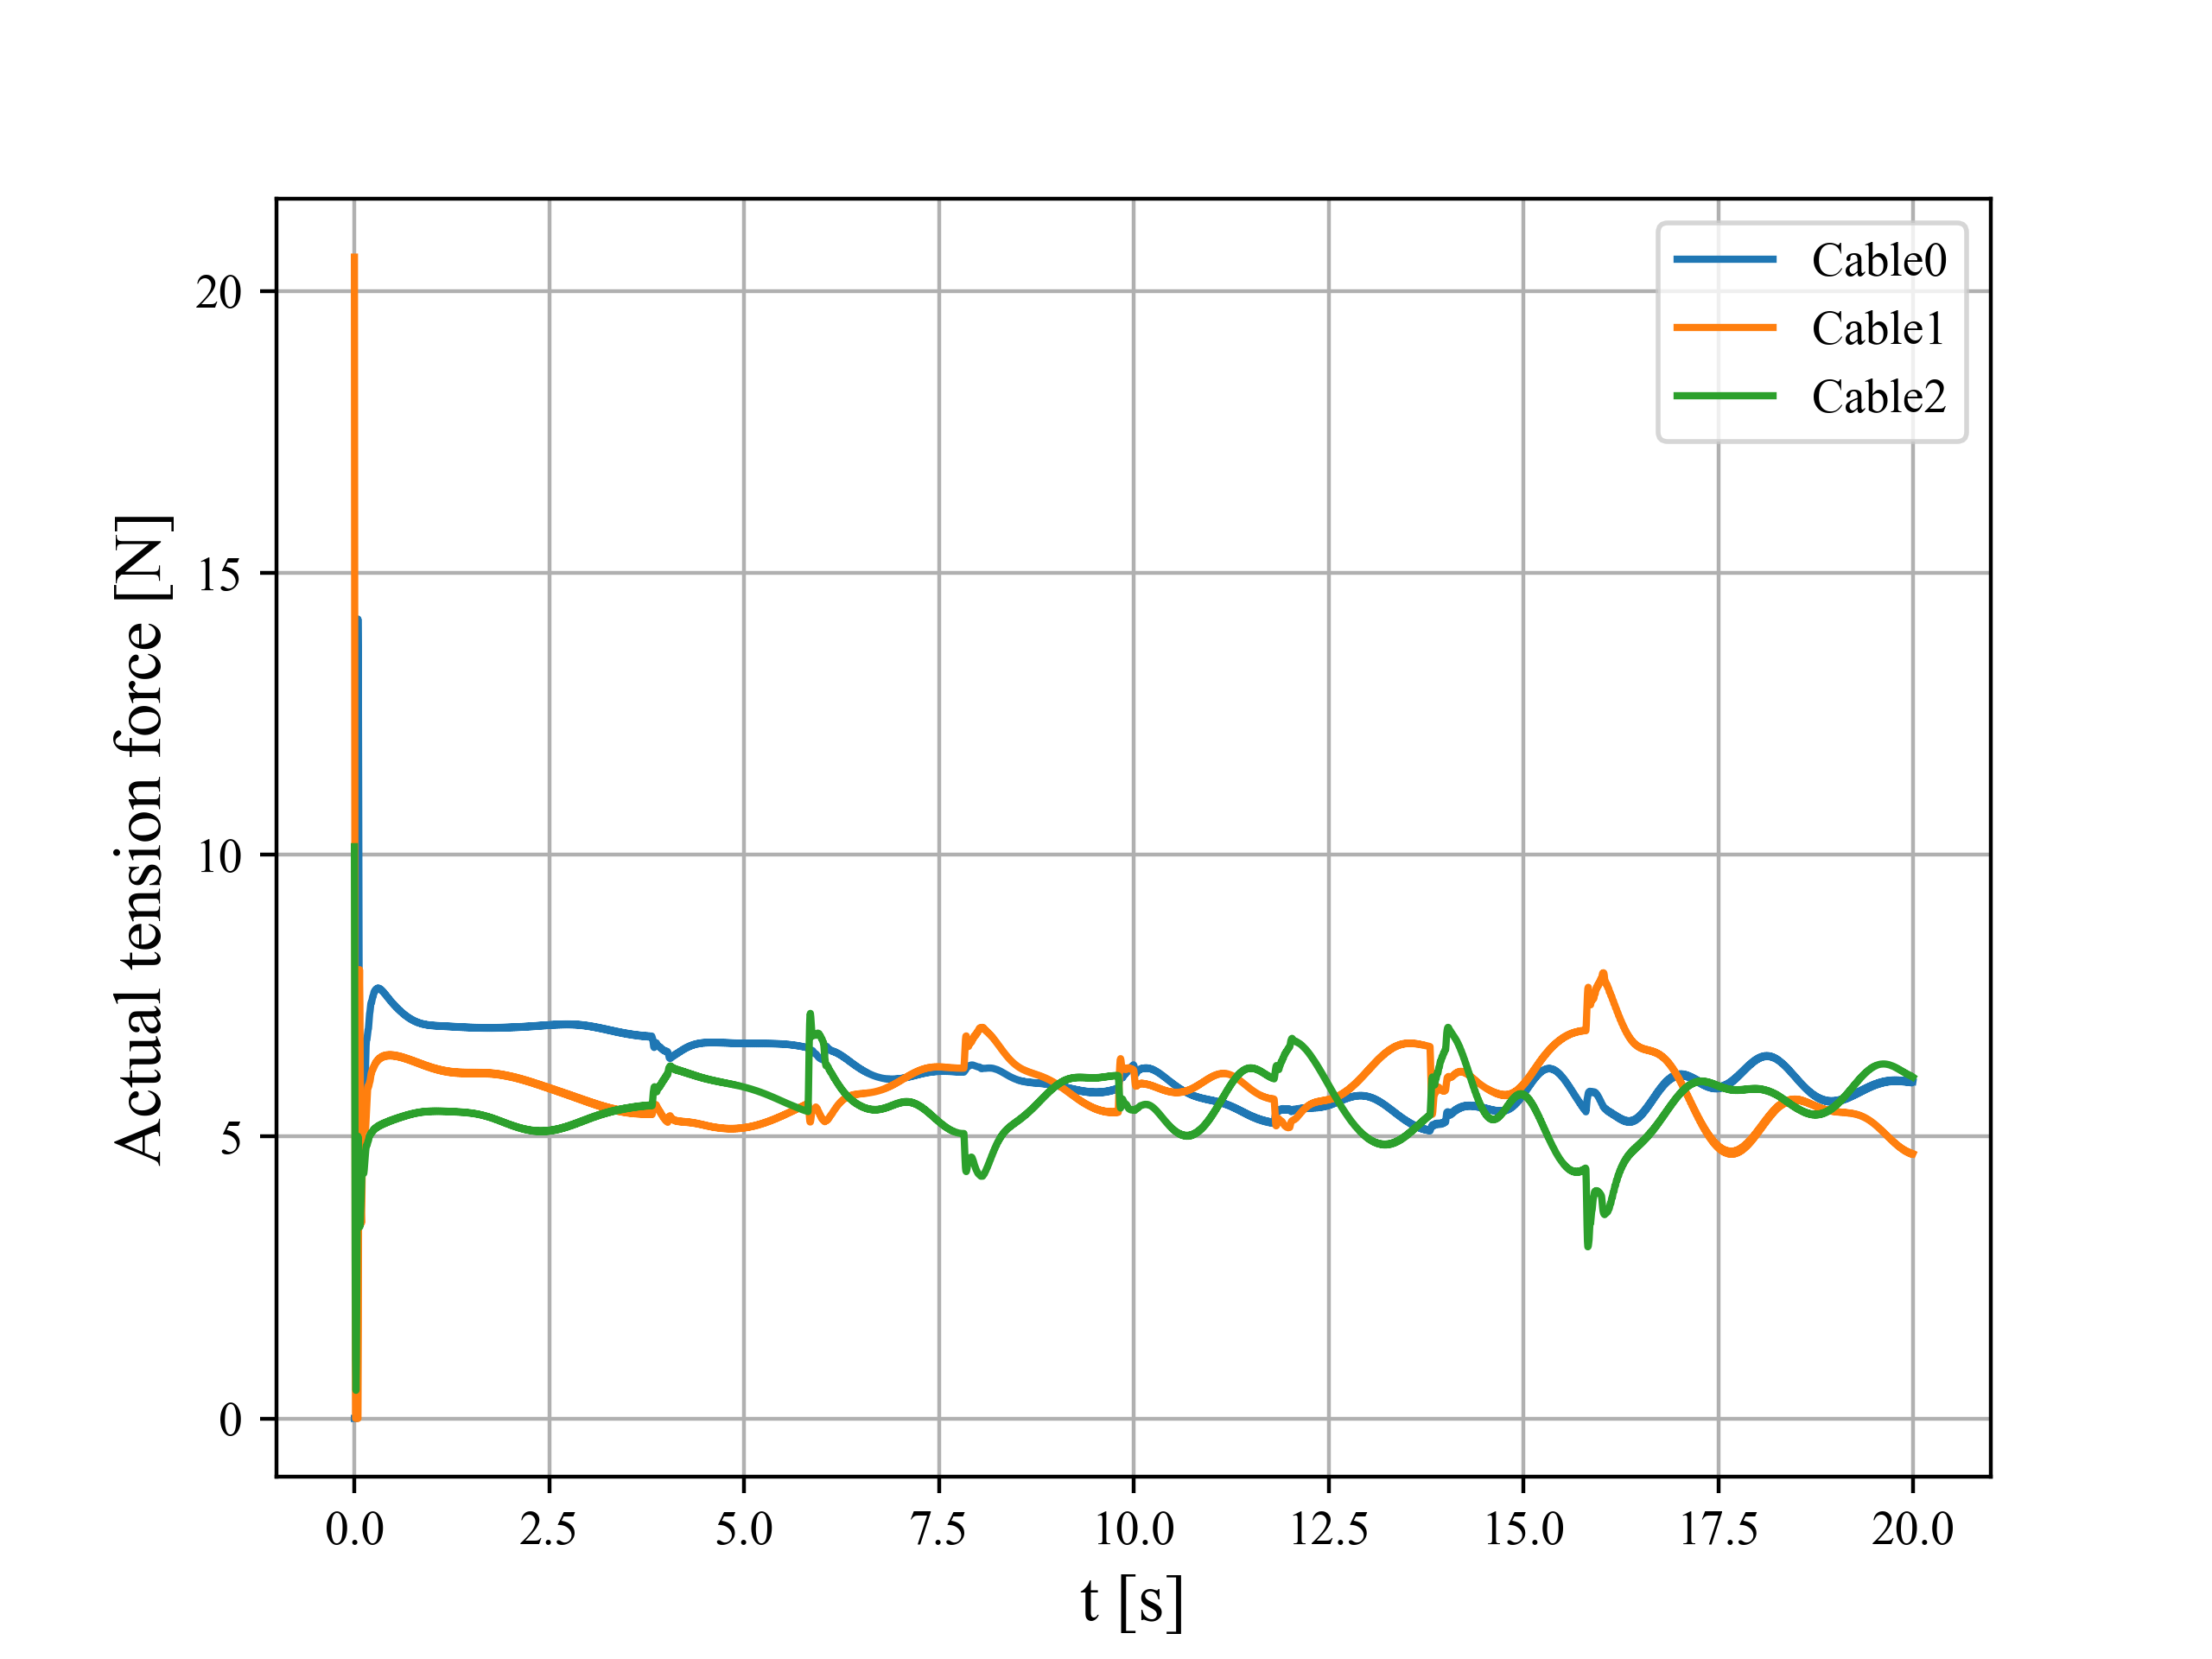
\includegraphics[width=\textwidth]{picture/kk/cable_actual_tensions_fig_8_6quad_ol.png}
        \caption{实际拉力}
        % \label{quadrotoru0}
    \end{subfigure}
    \hfill
    \begin{subfigure}[b]{0.48\textwidth}
        \centering
        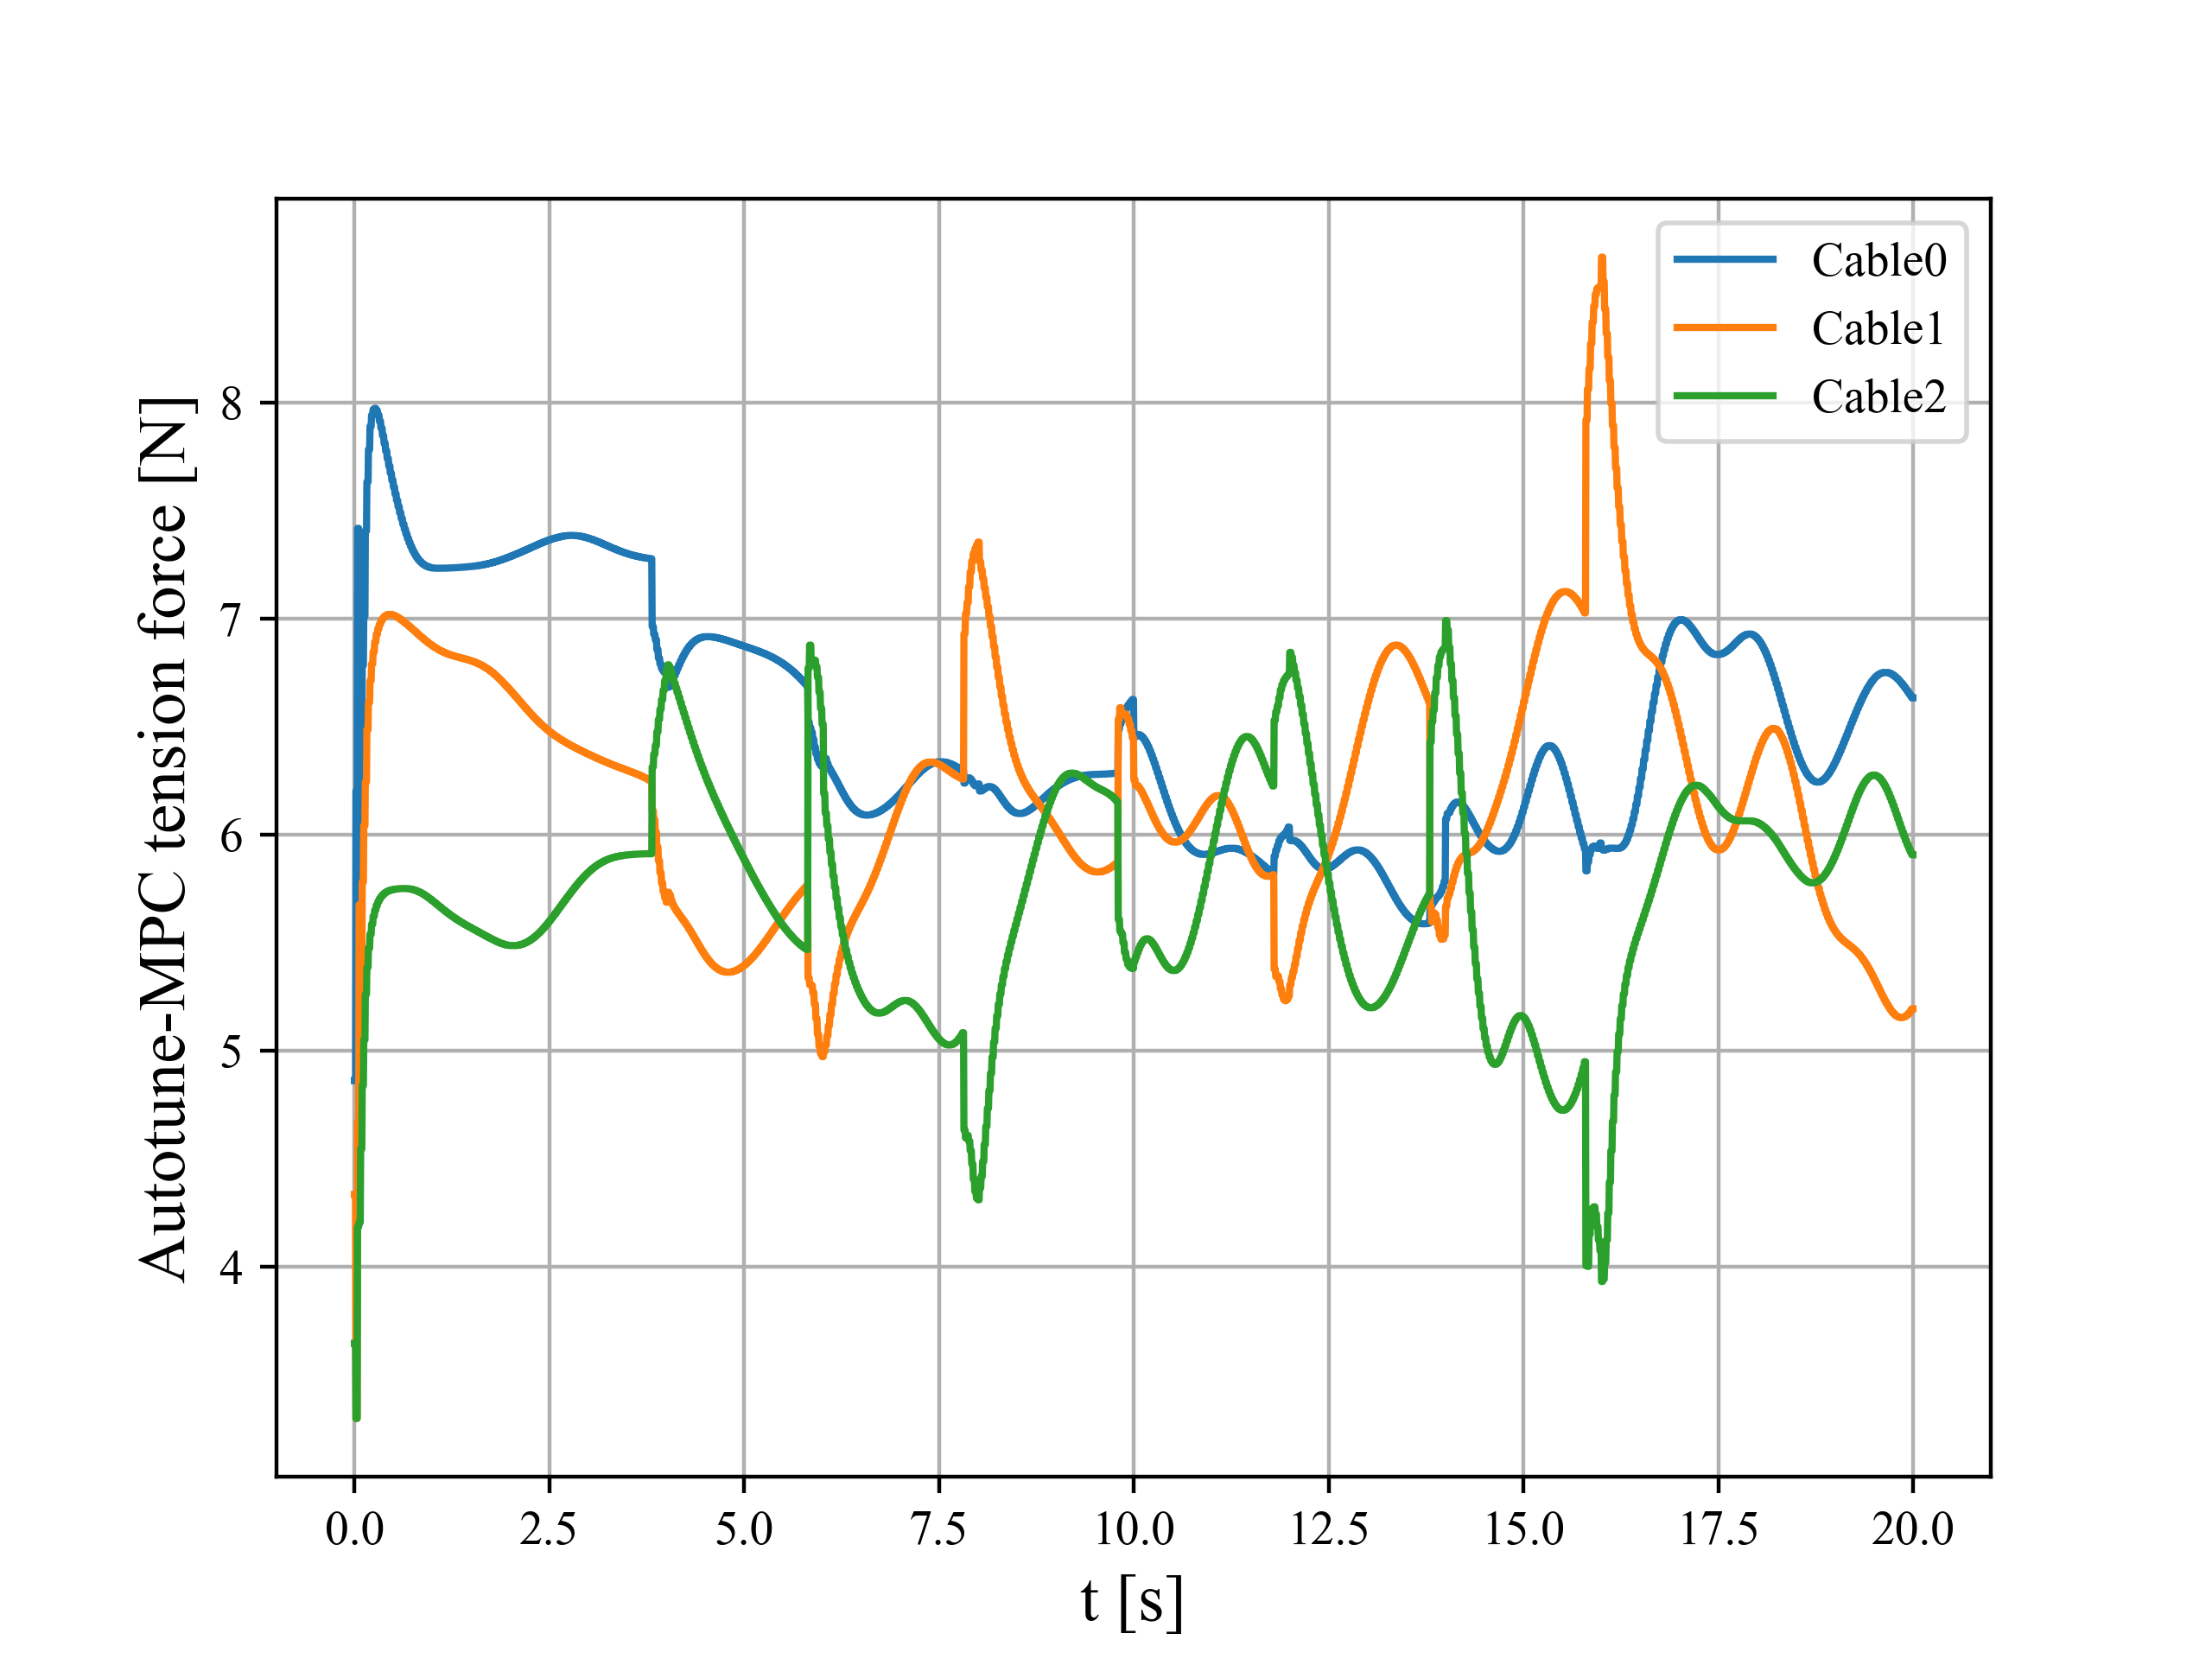
\includegraphics[width=\textwidth]{picture/kk/cable_MPC_tensions_fig_8_6quad_ol.png}
        \caption{MPC计算拉力}
        % \label{quadrotoru1}
    \end{subfigure}
	\caption{闭环训练过程中系绳上的拉力大小} 	
	\label{cjb1}
\end{figure}
% \subsection{梯度计算与实现}

% 针对上述参数化,链式法则~(15) 中的梯度计算公式重写为:
% \begin{equation}
%     \frac{d L_i}{d \pi_i} = \frac{\partial L_i}{\partial X_i^\text{cl}} \cdot \frac{\partial X_i^\text{cl}}{\partial \theta_i} \cdot \frac{\partial \theta_i}{\partial \Theta_i} \cdot \frac{\partial \Theta_i}{\partial \pi_i}, \quad \forall i \in \mathcal{I}_A.
% \end{equation}


\section{本章总结}
本文提出了一种自适应学习超参数优化算法——Autotune,用于多无人机绳系吊运系统。Autotune以分布式闭环方式自适应调整各种难以调整对自适应 MPC 超参数,通过引入分布式灵敏度传播算法计算系统状态相对于控制器关键参数的梯度,并通过分布式策略梯度算法更新生成的自适应归一化超参数。与现有的开环训练方法相比,Autotune具有具有收敛速度快、方便扩展等良好特性,且学习稳定性和闭环控制跟踪性能都有所提高。


\cleardoublepage

\chapter{物理引擎仿真与飞行试验验证}
\chaptermark{物理引擎仿真与飞行试验验证}
%为验证所提出方法的可行性与有效性,本章对章动目标消旋地面试验系统进行了搭建。试验系统主要由目标章动旋转模拟装置、磁场源、机械臂和计算机组成,通过目标章动模拟装置模拟空间目标的章动旋转运动,通过机械臂抓取磁场源模拟服务星的运动。采用不同消旋轨迹进行了多组试验,记录目标角速度变化情况并对结果进行了比较分析。
为了验证上述提出方法的可行性与有效性,通过物理引擎仿真和飞行试验验证两个方面对设计的算法效果进行评估。数据驱动方法依赖于大量高质量的标注数据来训练模型。然而,在机器人领域,获取真实世界的数据通常面临数据采集成本高、环境限制、数据标注困难等挑战,物理引擎仿真系统,可以在虚拟环境中高效生成大量多样化且精准标注的数据,避免了真实世界收集数据困难的问题。

在物理引擎仿真方面,在Drake、Gazebo和MuJoCo这几种主流仿真物理引擎平台中搭建无人机绳系吊运系统的动力学和环境模型,并选择最适合的物理引擎来模拟其飞行轨迹与响应特性。在飞行试验验证方面,基于实际硬件搭建无人机绳系吊运系统,通过物理引擎和真实试验收集的大量数据,在室内场景中完成一系列试验,验证仿真模型的准确性与适用性。本章通过物理引擎仿真和飞行试验的结合,为无人机绳系吊运系统的设计与优化提供了科学依据。
\section{物理引擎仿真系统介绍}
在无人机绳系吊运载荷系统的研究中,物理引擎仿真是通过计算机模拟现实世界现象的过程。不同的物理引擎模拟不同的现象,提供不同程度的逼真度,消耗不同数量的计算资源,并为不同的目的量身定制。低保真度的物理引擎通常所需的计算资源通常要少得多,因此通常用于快速估算真实世界的行为,或模拟系统的某个特定组件。相反,保真度较高的物理引擎可在一个或多个方面对真实世界的行为做出更准确的估计。

本章选用了几种主流物理仿真平台对无人机绳系吊运系统的深入分析和验证,包括Drake、Gazebo和MuJoCo。这些平台具有高效的物理建模和仿真功能,可以满足复杂动力学系统建模及仿真精度的需求。本节将对仿真系统的构建流程、各平台的特点及其在仿真中的具体应用进行详细介绍。

\subsection{Drake仿真引擎}
Drake 是由麻省理工学院计算机科学与人工智能试验室与丰田研究院联合开发的一款功能强大的开源物理仿真与控制工具,专注于动力学建模、优化及精确控制仿真。它广泛应用于机器人动力学的分析以及控制系统的开发,特别适合研究高自由度系统。Drake 使用高精度数值积分方法,确保动力学计算的准确性,可模拟包括摩擦、接触、空气动力学在内的复杂机器人动力学,并将这些信息传递给高级规划、控制与分析算法。此外,Drake 提供符号计算与解析梯度支持,对于优化控制和建模复杂任务至关重要。

与 Simulink 类似,Drake 强调模块化设计,具备灵活的接口和先进的数学工具,是学术研究和工业应用的理想选择。其高效的优化工具可用于验证控制算法并优化其性能。

Drake 工具箱提供了以下三大核心组件,用于实现高效、灵活的动力学系统建模:

(1)动态系统建模:Drake 的核心功能包括通过多种动力学组件构建系统模型,这些组件涵盖传感器、执行器、估计器和控制器等模块,满足复杂系统建模的需求。

(2)多体运动学与动力学:Drake 支持解析多种运动学模型格式,可对多体系统进行运动学仿真,同时支持接触建模,实现精确的动力学计算。

(3)数学程序求解:Drake 提供统一的接口支持多种数学规划求解器,能够解决复杂的优化问题,包括路径规划、控制优化和系统稳定性分析。

\begin{figure}[hbt!]
	\centering
	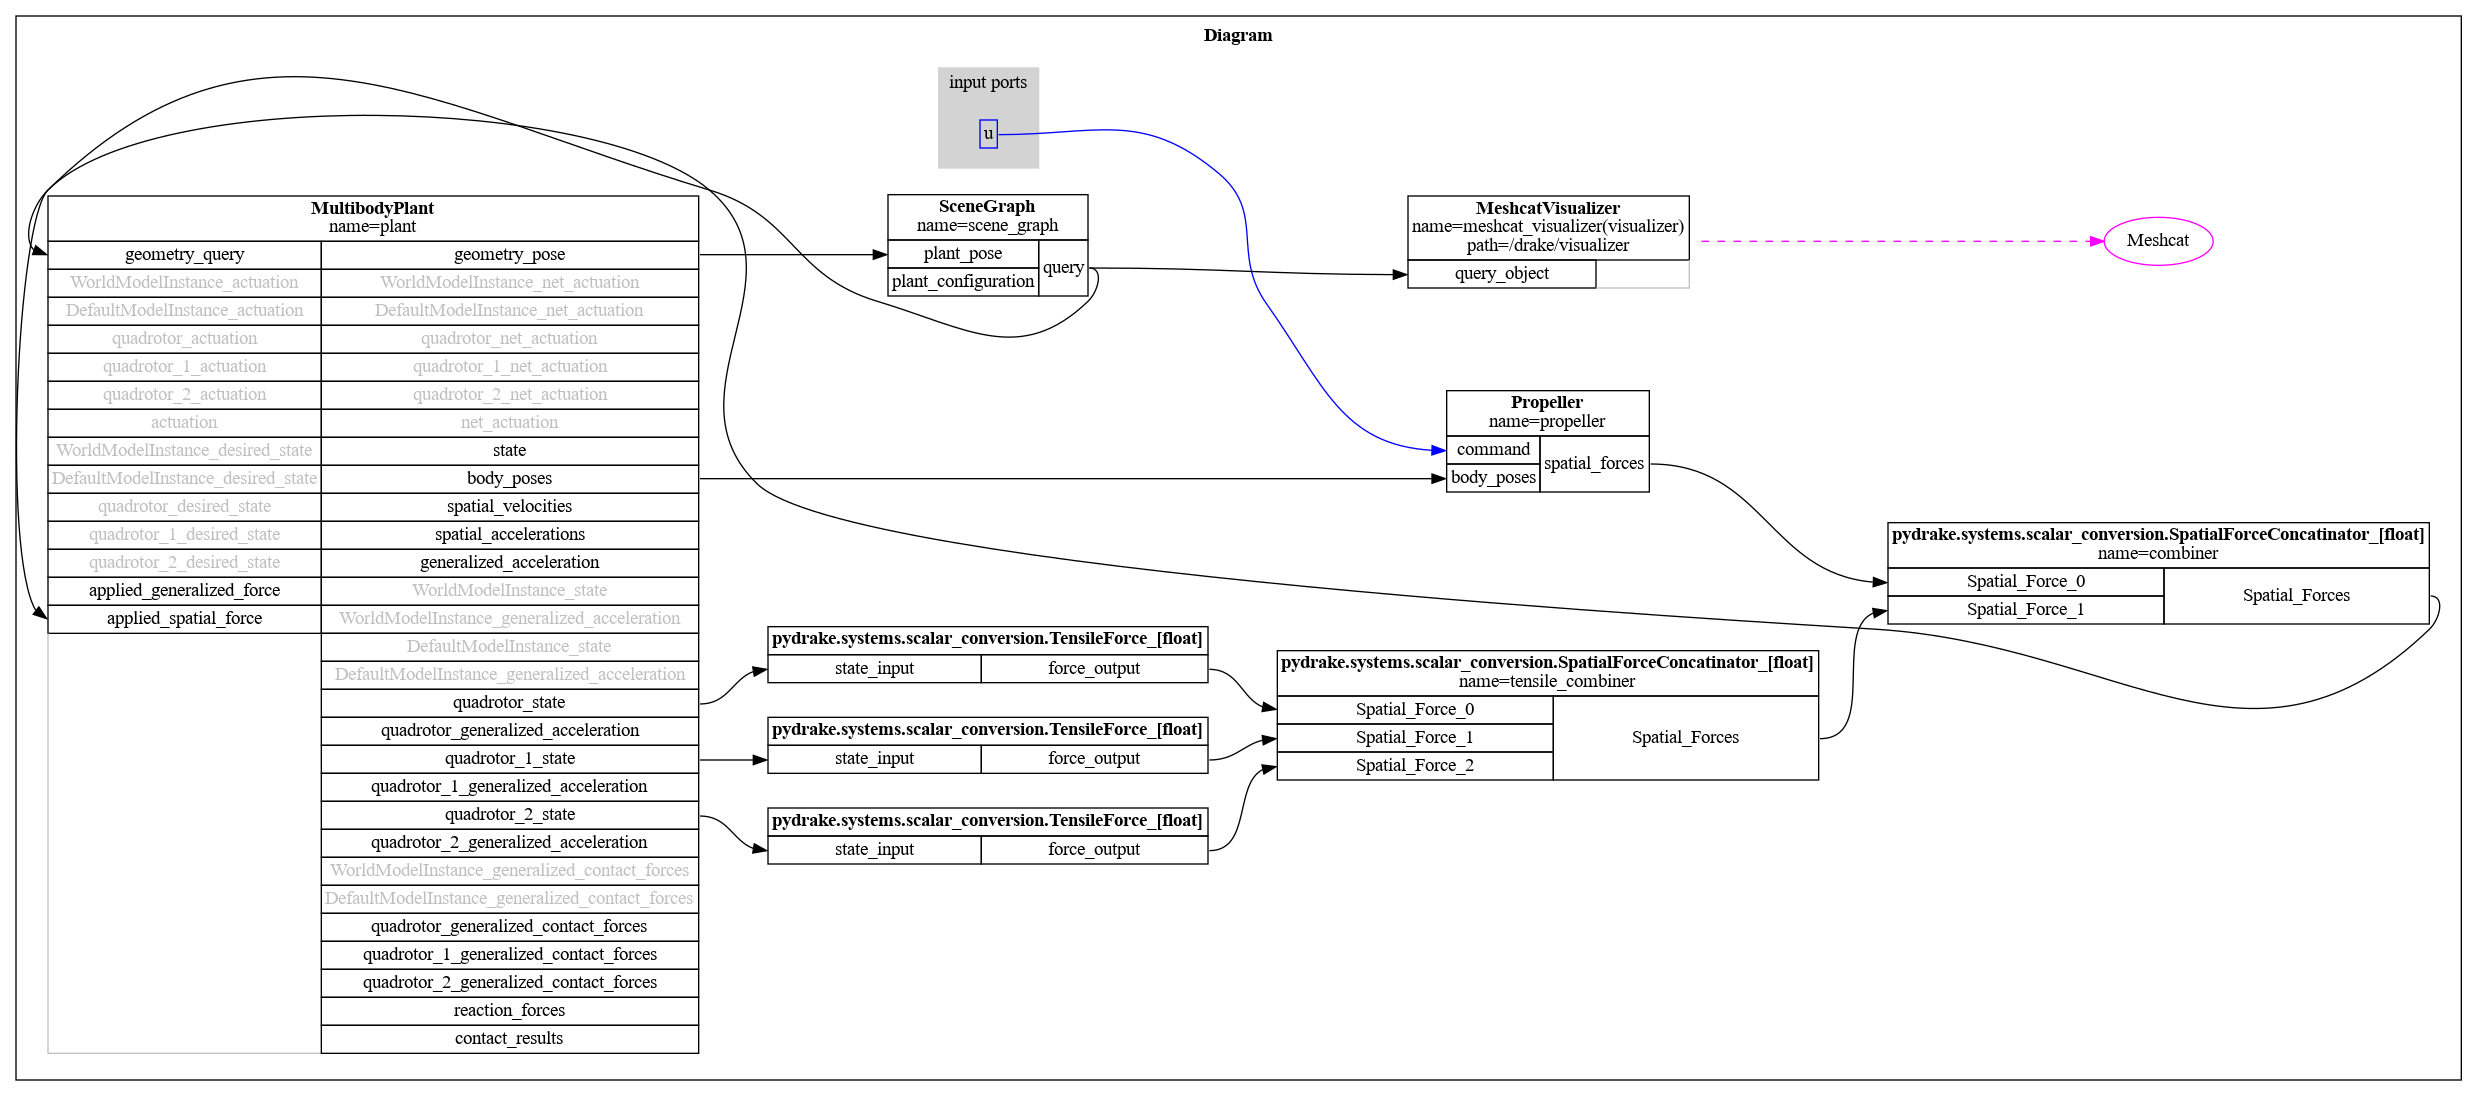
\includegraphics[width=38pc]{picture/drake.png} 
	\caption{Drake仿真引擎中三架无人机系统流程框图} 
	\label{drake}
\end{figure}
在最初的设计中,无人机绳系吊运系统采用多路复用器和解复用器来拼接系统的输入与输出。然而,这种方法容易导致状态变量之间的混淆问题。为解决此问题,系统设计进行了改进:移除多路复用器和解复用器,直接将三架无人机的 12 个输入传递给系统,并输出三架无人机的所有状态变量,系统的结构如图 \ref{drake} 所示。此外,为每架无人机添加了滚转-俯仰-偏航关节。相较于单架无人机的设计,系统中对角权重矩阵 $Q$和控制权重矩阵 $R$的长度增加了 3 倍,但其组成方式保持不变。

\begin{figure}[hbt!]
	\centering
	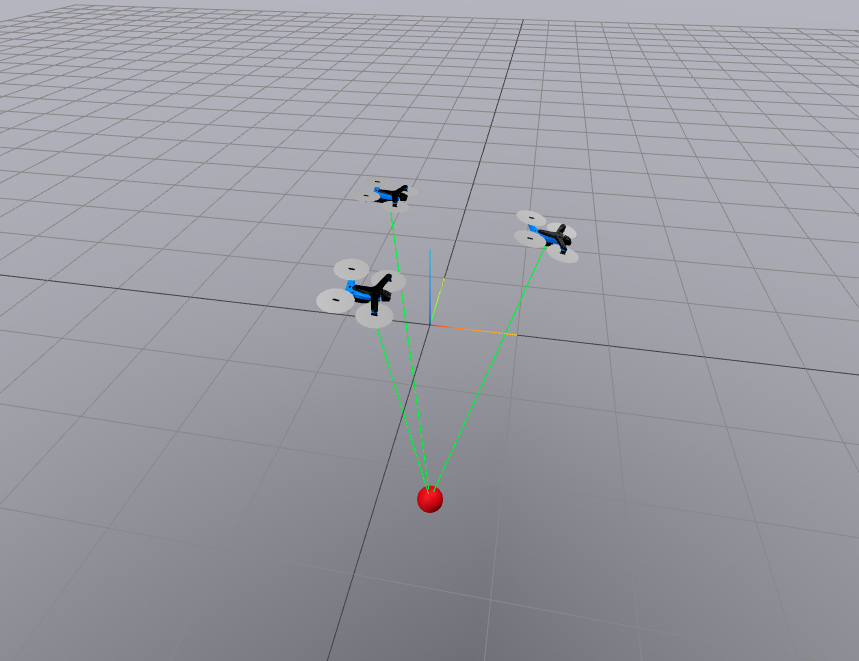
\includegraphics[width=36pc]{picture/5_1.png} 
	\caption{Drake仿真引擎中的多无人机绳系吊运系统} 
	\label{5_1}
\end{figure}
在系统建模过程中,通常使用机器人描述格式文件(URDF),结构化地描述模型的各个部分,并清晰定义系统的动力学属性。在 Drake 中,URDF 文件通过定义传感器、执行器和多体结构等实现精确的仿真建模。该系统的动力系统组件还通过增加螺旋桨和控制器模块进一步增强了建模能力。


Drake 目前主要支持刚体物体的模拟,对于柔性物体(如系绳)的建模需采用简化方法。为解决该问题,系绳被建模为弹簧,其拉伸状态根据系统状态施加力。具体而言,系绳行为简化为弹簧模型,在拉紧时施加力,而松弛时不施加任何力。此方法虽然简化了系绳的物理特性,但在一定程度上仍能反映其在系统中的作用。这种建模方式引入了系统的混合组件,其中弹簧模型与刚体物体的相互作用构成混合系统。当系绳处于拉伸状态时,施加的弹性力不同于传统刚体动力学行为,因此需作为特殊约束条件处理。尽管 Drake 不直接支持柔性物体建模,但通过此方法,仿真中依然可以实现系绳的作用,并与其他刚体物体的动力学交互。

此外,Drake 集成了轻量级的 Web 3D 可视化工具 Meshcat,为开发者提供交互式的可视化功能,便于调试、展示与分析仿真结果,如图 \ref{5_1} 所示。通过 Meshcat,开发者可以实时观察复杂系统的运行状态,从而大幅提高开发效率。

\subsection{Gazebo仿真引擎}
如果仿真任务涉及到复杂的物理约束和要求极高的精度,Drake 通常是首选工具。然而,Drake 的缺点在于它的计算复杂度较高,尤其是当仿真规模增大时,计算资源的消耗也随之增加,因此它可能不适合需要快速仿真或大规模环境模拟的场景。

Gazebo 是一个通用的开源仿真框架,它将刚体物理引擎(与图形用户界面(GUI)相结合,并提供了丰富的插件,支持复杂的三维环境建模和模拟各种机器人组件(如电动机、受空气动力学力影响的螺旋桨、传感器噪声及摄像头等)。类似于 Drake,Gazebo 也能处理通过 SDF 文件定义的多无人机绳系吊运系统,并进行动态交互。对于无人机仿真,Gazebo能够通过插件实现气动力、重力以及绳系约束的精确建模。
然而,Gazebo 与Drake一样,仅能模拟刚体物体。这意味着系绳需要通过多串联链来进行建模。影响系绳模型精度的五个关键参数如下:

(1){链节数量}:每根系绳由多少个刚性圆柱体组成。增加链节数量可提升模型的逼真度,但也会增加计算资源消耗。经验表明,使用 10 个链节足以在搭载 i5-1135G7 CPU 和 16 GB 内存的 Intel NUC 计算机上实现较高精度且不会带来过大计算压力。
    
(2){关节类型}:选择合适的关节类型(如球形关节、滑动关节或万向节)。由于柔性系绳不具备刚性关节,约束最少的球形关节是最佳选择。
    
(3) {关节阻尼系数}:描述关节运动过程中的能量损失速率。较大阻尼系数会减少能量传输,而较小阻尼系数可能引发不稳定振荡。试验表明,$0.01 \text {N}\cdot \text{s} \cdot \text{m}^{-1}$ 是最优阻尼系数。低于该值会导致系绳振荡至不稳定状态,高于该值则影响运动传递效果。
    
(4){关节摩擦系数}:描述关节运动时需克服的摩擦力。由于柔性系绳不含刚性关节,任何摩擦系数的加入都会使模型过于刚性。因此,摩擦系数设为 0。
    
(5) {碰撞几何体}:确定碰撞检测的位置。由于无人机的配置和准静态操作方式,系绳与外部环境的碰撞极少发生,主要例外情况是起飞前与地面的接触。考虑到碰撞建模计算量较大,且大多数情况下系绳不会发生显著碰撞,因此碰撞几何体被禁用。

\begin{figure}[hbt!]
	\centering
	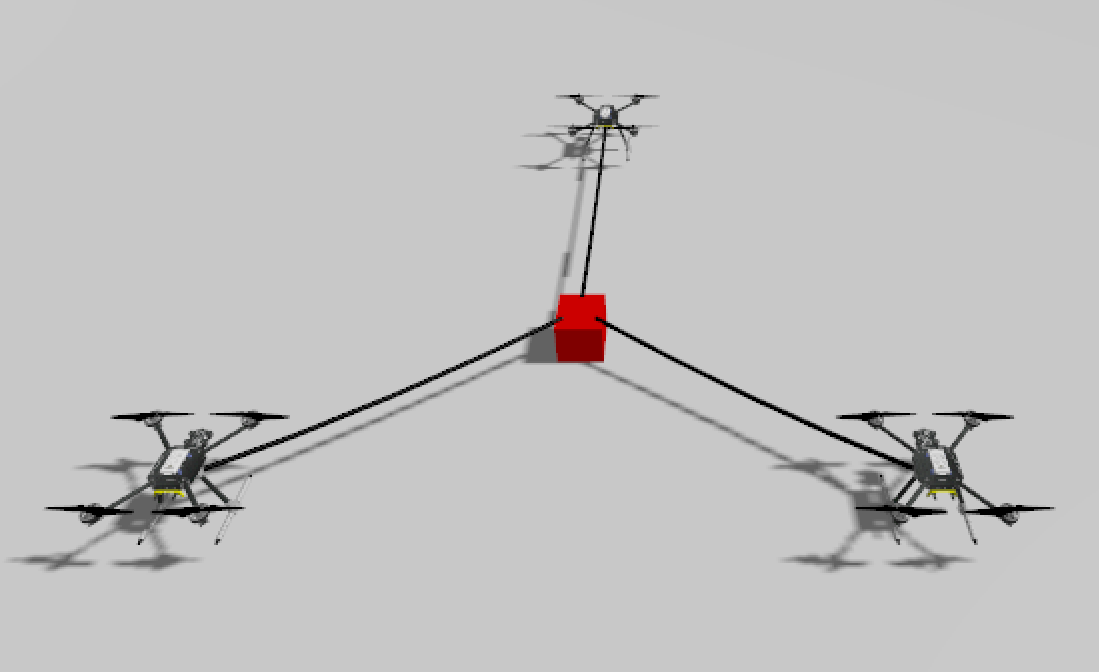
\includegraphics[width=36pc]{picture/5_2.png} 
	\caption{Gazebo仿真引擎中的多无人机绳系吊运系统} 
	\label{5_2}
\end{figure}
图 \ref{5_2} 显示了用于三架无人机和载荷系统的完整SDF(Simulation Description Format) 模型。该模型包含三根系绳,每根系绳由离散的链接刚体构成,两端通过球形接头连接。每根系绳都由 XACRO 文件生成,因此可以方便地调整其长度、质量和链接数。载荷被模拟为一个球体,系绳连接点沿中心平面对称分布,以模拟载荷的刚体特性。系绳连接到无人机的质量中心。

\begin{figure}[hbt!]
	\centering
	\begin{subfigure}[t]{0.9\textwidth}
		\centering
		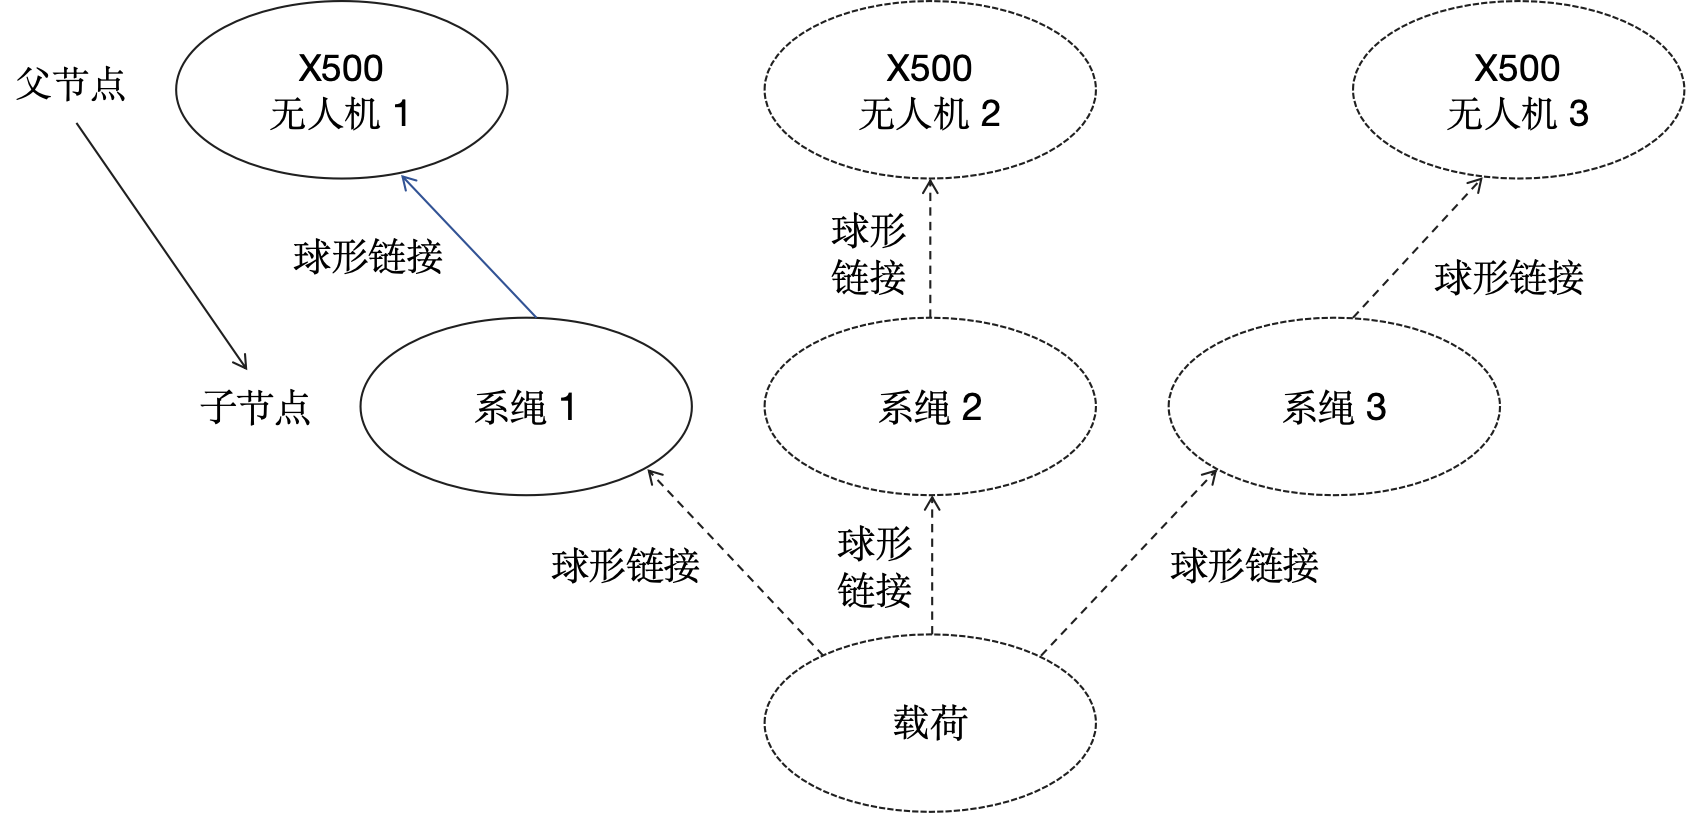
\includegraphics[width=0.8\textwidth]{picture/tree2.png}
		\caption{无人机为父节点}
		\label{tree1}
	\end{subfigure}\\[2ex] % 使得两图之间有一点间距
	\begin{subfigure}[t]{0.9\textwidth}
		\centering
		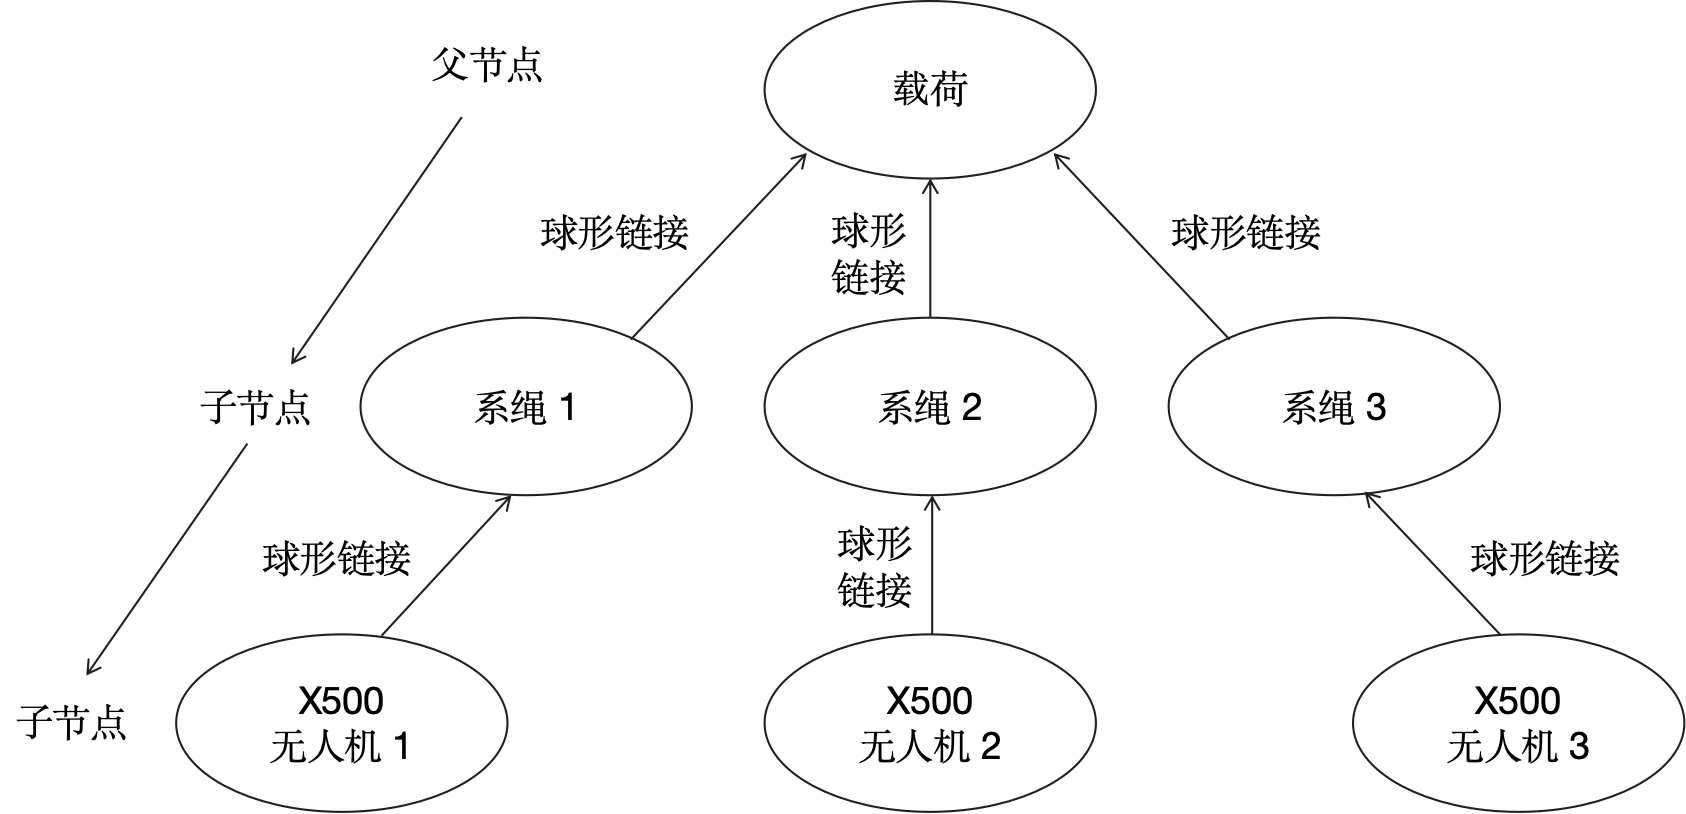
\includegraphics[width=0.8\textwidth]{picture/tree1.png}
		\caption{载荷为父节点}
		\label{tree2}
	\end{subfigure}
	\caption{由无人机、系绳和载荷构成的树图}
	\label{tree_combined}
\end{figure}
在 SDF 文件中,父节点指运动学树中上层的节点(link),作为其他节点的基准或连接点。父子关系通过 <parent> 和 <child> 标签表示,父节点控制系统运动,子节点通过关节(joint)与其相连,形成多体动力学系统。系绳由多个链接组成,但在模型中简化为单一链接,并通过球形铰链连接至无人机质量中心。

对于多无人机绳系吊运系统来说,首先设置父节点为无人机,子节点为系绳和载荷(见图 \ref{tree1})。这是采用类似倒车摆的方式来解决问题,且该方法在网上有较为完善的文档。但是在多无人机绳系吊运系统中,由于多个无人机的存在,只能实现单无人机的绳系吊运系统,当添加载荷和另外两架无人机时,遇到了错误(用虚线表示)。
因此,设置载荷为父节点,随后是系绳和无人机作为子节点(见图 \ref{tree2}),从而构建得到完整的无人机绳系吊运系统SDF文件。

在 Gazebo 仿真环境中集成了开源无人机飞控系统 PX4,可以通过 SITL(Software In The Loop)仿真模式进行测试。SITL 仿真指将编译好的嵌入式代码在开发计算机上运行,而非最终硬件上执行,使开发者无需实际硬件即可测试和调试飞控系统。开发计算机运行 PX4 代码,并与仿真环境交互,模拟传感器输入与执行器输出。

此外,Gazebo 可通过 ROS2(Robot Operating System 2)集成,为仿真环境提供强大的通信与控制功能。ROS2 使无人机控制算法能够与仿真机器人系统无缝对接,简化开发流程,提高验证效率与准确性。开发者可借助 ROS2 实现与多种硬件接口的交互,同时控制仿真机器人,如导航与姿态控制。

Gazebo 仿真环境能精确模拟多无人机吊装系统中的传感器(如 IMU、GPS、视觉传感器)、执行器(如电机、舵机)及多体动力学行为。高保真仿真可再现实际系统动态表现,包括风力、地形和外部干扰,帮助开发者真实验证算法性能与鲁棒性。开发者可在虚拟环境中进行飞行路径规划、控制算法优化和系统评估,无需昂贵的硬件测试。

该仿真方法的优势在于开发者能够在复杂场景下快速迭代与测试,无需实际硬件部署。仿真中可尝试不同控制策略、调整参数并实时观察系统响应,优化算法与飞行策略。此外,该集成方式有助于在软件部署至实际硬件前发现潜在问题,降低开发风险与成本。

\subsection{MuJoCo仿真引擎}
在以上两种仿真引擎中,Drake通过弹簧对系绳进行建模,Gazebo则是通过多链刚体对系绳建模,这两种建模方法在一定程度上都不能够模拟真实的柔性系绳,这也突显了寻找一种既精确又计算开销低的系绳动态建模方法的必要性。

MuJoCo 是一款高保真开源物理引擎,专注于复杂多体动力学仿真,广泛应用于机器人学、控制理论、仿真优化和虚拟现实等领域。其以高精度数值计算和精细的柔性体、接触力学建模著称,在系绳、布料和可变形物体等柔性系统的仿真中表现出色。

MuJoCo 的核心优势之一是其对柔性体的建模能力,能够准确模拟软体与硬体的交互以及动态环境下的柔性结构响应,适用于复杂的系绳吊运和柔性机器人系统仿真。

\begin{figure}[hbt!]
	\centering
	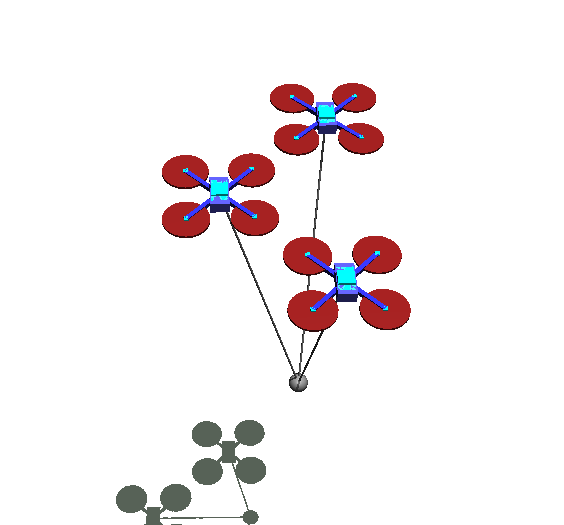
\includegraphics[width=34pc]{picture/5_3.png} 
	\caption{MuJoCo仿真引擎中的多无人机绳系吊运系统} 
	\label{5_3}
\end{figure}

为了增强仿真结果的可视化与交互,MuJoCo 提供了与外部可视化工具(如 OpenGL)集成的能力,允许开发者实时观察仿真过程中的系统状态如图 \ref{5_3} 所示。这种高度交互性和可视化能力大大提升了开发者在测试和调试过程中的效率。

MJCF(MuJoCo XML Format)是 MuJoCo 仿真引擎中用于定义系统模型的标准化文件格式。与 SDF 文件不同,MJCF 文件在描述机器人结构时不是用父节点和子节点的方式,而是通过直接的嵌套表示其父子关系。MJCF不仅能表示机器人本体信息,还能表示环境信息,其主体并不是系统本身,而是整个世界,里面可以可嵌套多个系统。

\begin{figure}[hbt!]
	\centering
	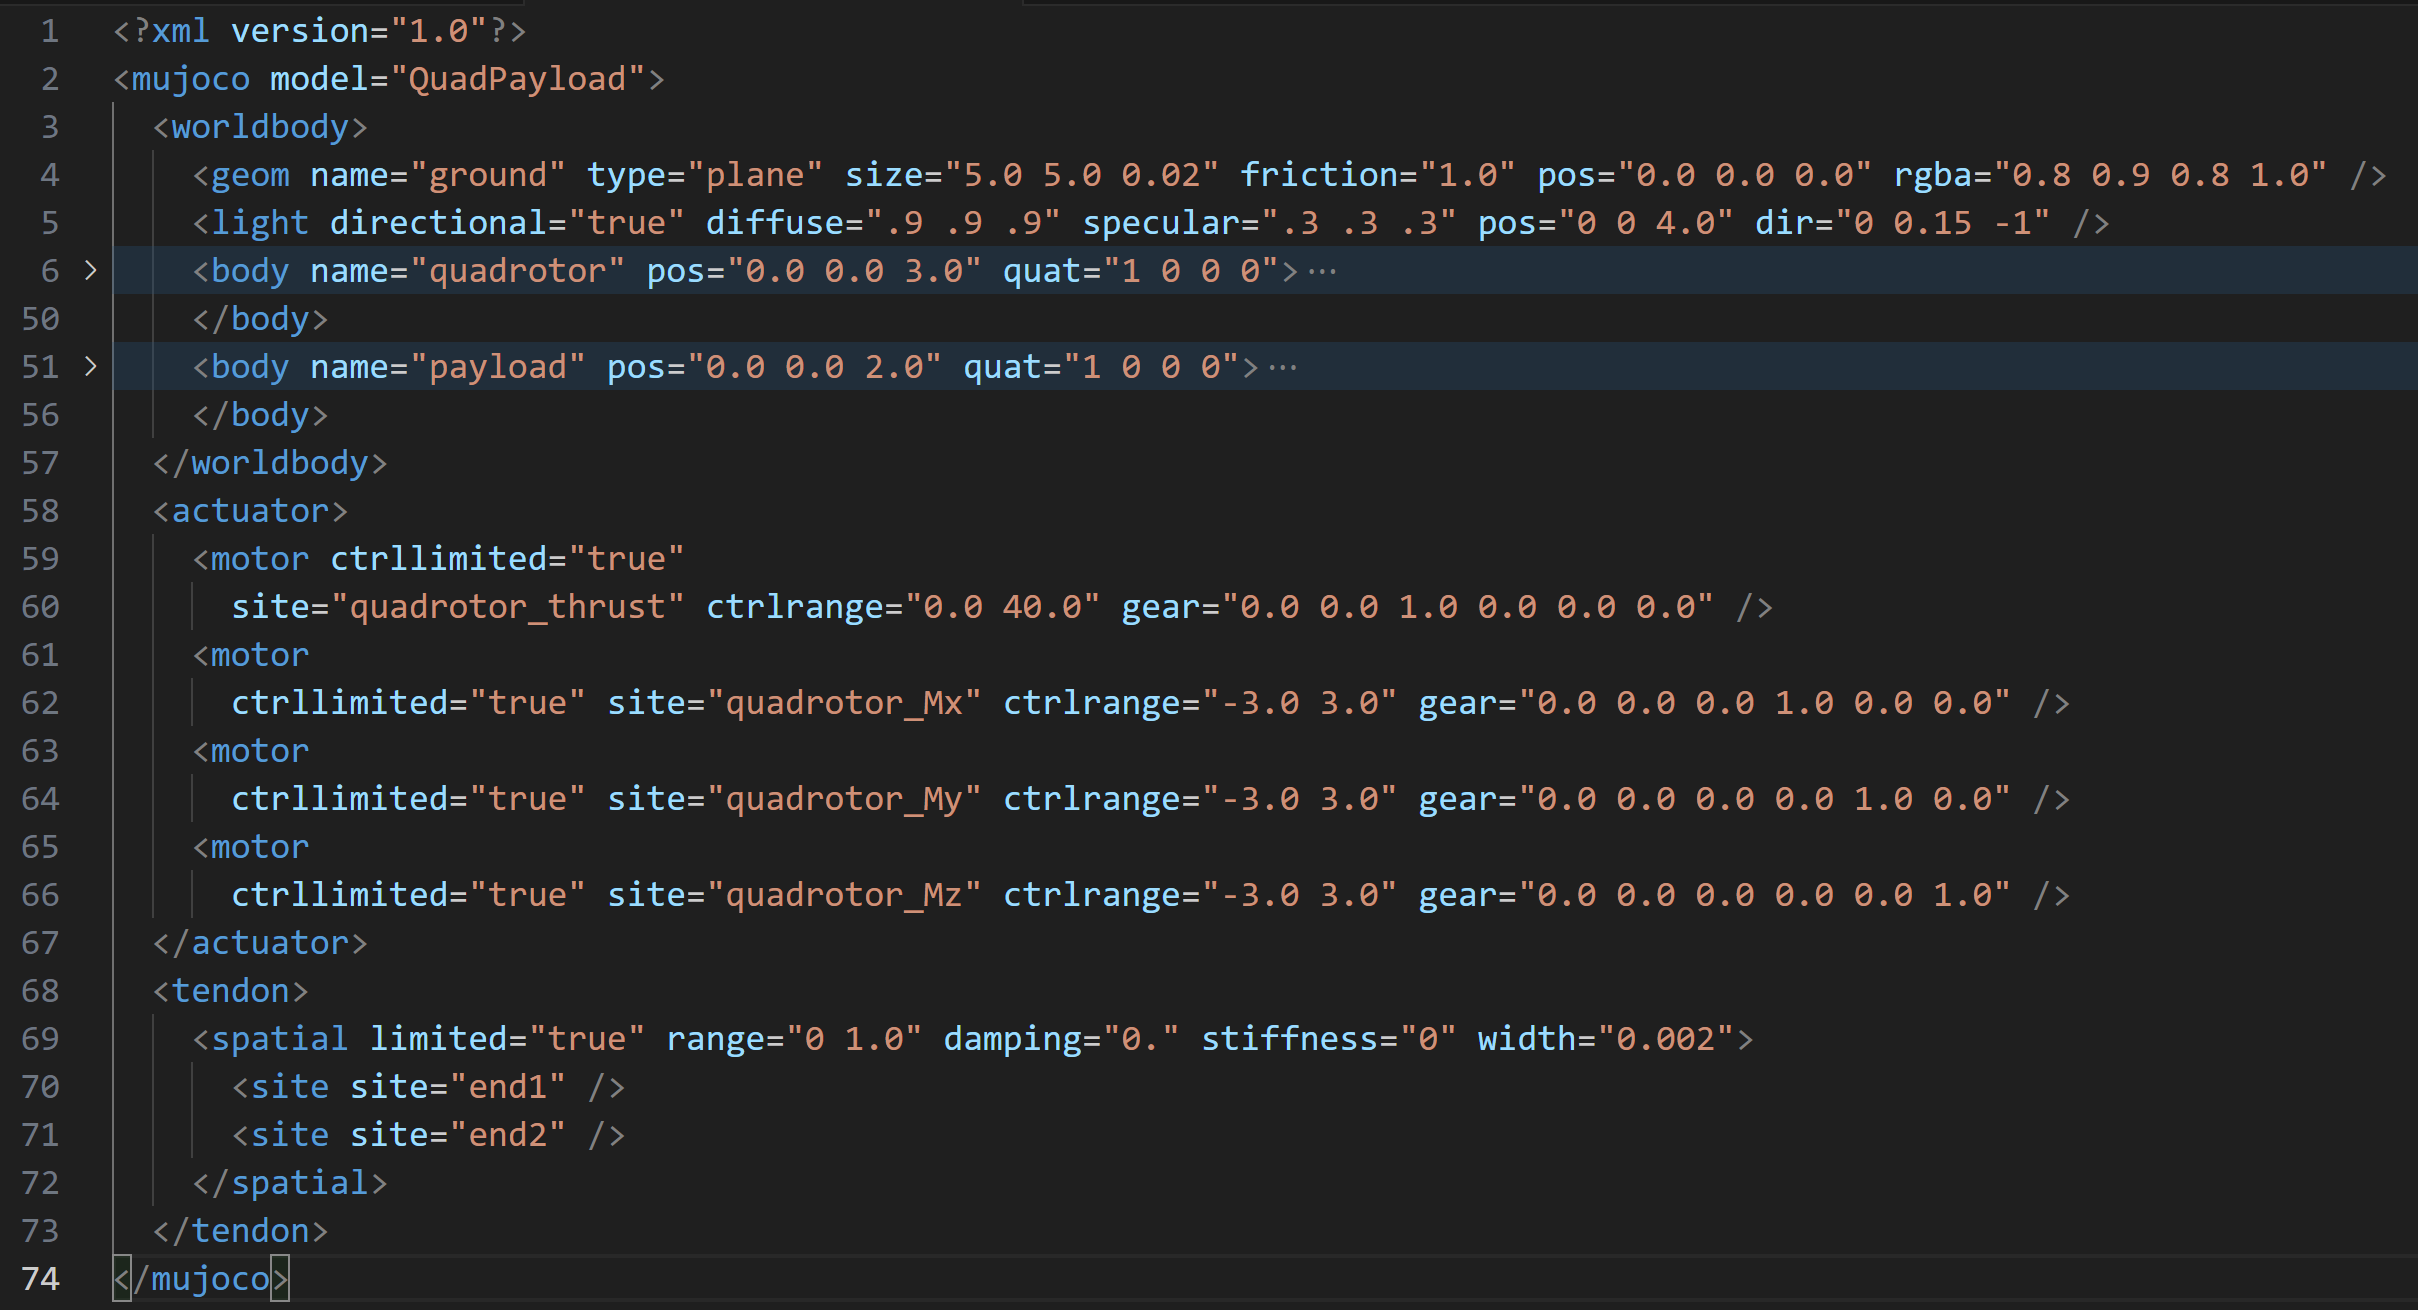
\includegraphics[width=36pc]{picture/MJCF.png} 
	\caption{无人机绳系吊运系统的 MJCF文件} 
	\label{MJCF}
\end{figure}
如图 \ref{MJCF} 所示,MJCF 文件使用 XML 语法,详细描述无人机绳系吊运系统的组成部分,包括物体的几何形状、动力学属性、约束条件和接触模型等,是 MuJoCo 中进行建模与仿真的核心工具之一。它为仿真引擎提供了一种灵活且易于扩展的方式来描述复杂的动力学系统。
MuJoCo 中的 sensor 组件可用于创建传感器并将其附加到模型的特定部分,为仿真中的无人机配置虚拟传感器,将传感器数据反馈到控制系统中进行处理,从而为无人机的自主飞行算法提供实时反馈。
MuJoCo 的 tendon 组件为模拟柔性组件(如系绳)提供了强大且灵活的功能。通过设置拉伸刚度、阻尼和连接的关节,tendon 组件能够有效地将柔性动力学融入到刚体动力学仿真中,极大地便利了复杂系统的建模。


\subsection{仿真引擎对比}
在无人机绳系吊运系统的仿真中,Drake、Gazebo和MuJoCo这三种仿真引擎各具特点,适用于不同的应用场景。Drake以高精度的动力学模拟著称,特别适合需要精细控制与优化的系统,在多体动力学和高自由度系统方面表现突出。然而,Drake在柔性物体建模上存在局限,通常采用简化的弹簧模型进行系绳仿真,可能无法完全捕捉柔性组件的复杂动态行为。Gazebo在快速仿真和大规模环境建模方面具有优势,尤其适合与ROS集成的应用。它支持多种复杂的三维环境建模和各种机器人组件的模拟,但对于柔性物体的仿真,Gazebo依赖于刚体物体的链式建模,精度相对较低。MuJoCo在无人机绳系吊运系统的仿真中展现出独特优势,特别是在柔性物体的精确建模方面。它允许用户定义精确的刚性体与柔性体属性、摩擦系数、接触参数等,能够准确模拟系绳等柔性组件的动态行为,提供高保真的仿真结果。此外,MuJoCo提供了灵活的建模方式,允许用户定制复杂的动力学系统,特别是在涉及柔性部件与刚性系统耦合的场景下,为无人机绳系吊运系统的研究提供了强大的支持。

\section{Mujoco下的无人机绳系吊运系统控制仿真验证}
如上一小节所述,MuJoCo 由于其在精确模拟柔性系绳动态行为方面的优势,在无人机绳系吊运系统的应用中明显优于 Gazebo 和 Drake。在本小节中,将采用 MuJoCo 作为仿真平台,进行无人机绳系吊运系统的控制仿真与验证,以评估其在复杂动态环境中的表现与性能,验证其在实际应用中的可行性与优势。

\subsection{单无人机吊运仿真验证}
在单无人机吊运仿真仿真中,无人机和有效载荷的质量分别为0.75 kg和0.15 kg,无人机的转动惯量通过MJCF中的“inertiafromgeom”模块自动计算得到。无人机与有效载荷之间的吊绳长度为1m。在仿真中,使用显式Runge-Kutta数值积分法,采样时间为0.01s,用于模拟系统的动态响应。
通过悬停与轨迹跟踪两个仿真对设计的NP-MPC算法进行了验证。Neural Predictor的训练数据通过在仿真环境中生成的圆轨迹和双纽线轨迹中进行收集,轨迹速度和半径均为随机值。共收集了1000条轨迹,每条轨迹持续20s,包含2000个数据点。
\begin{figure}[hbt!]
	\centering
	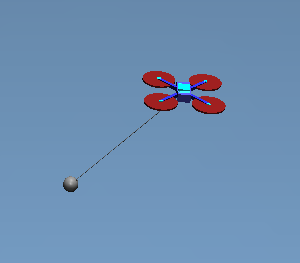
\includegraphics[width=25pc]{picture/kk/xuanting.png} 
	\caption{无人机悬停仿真场景} 
	\label{xuanting}
\end{figure}

\begin{figure}[hbt!]
	\centering
	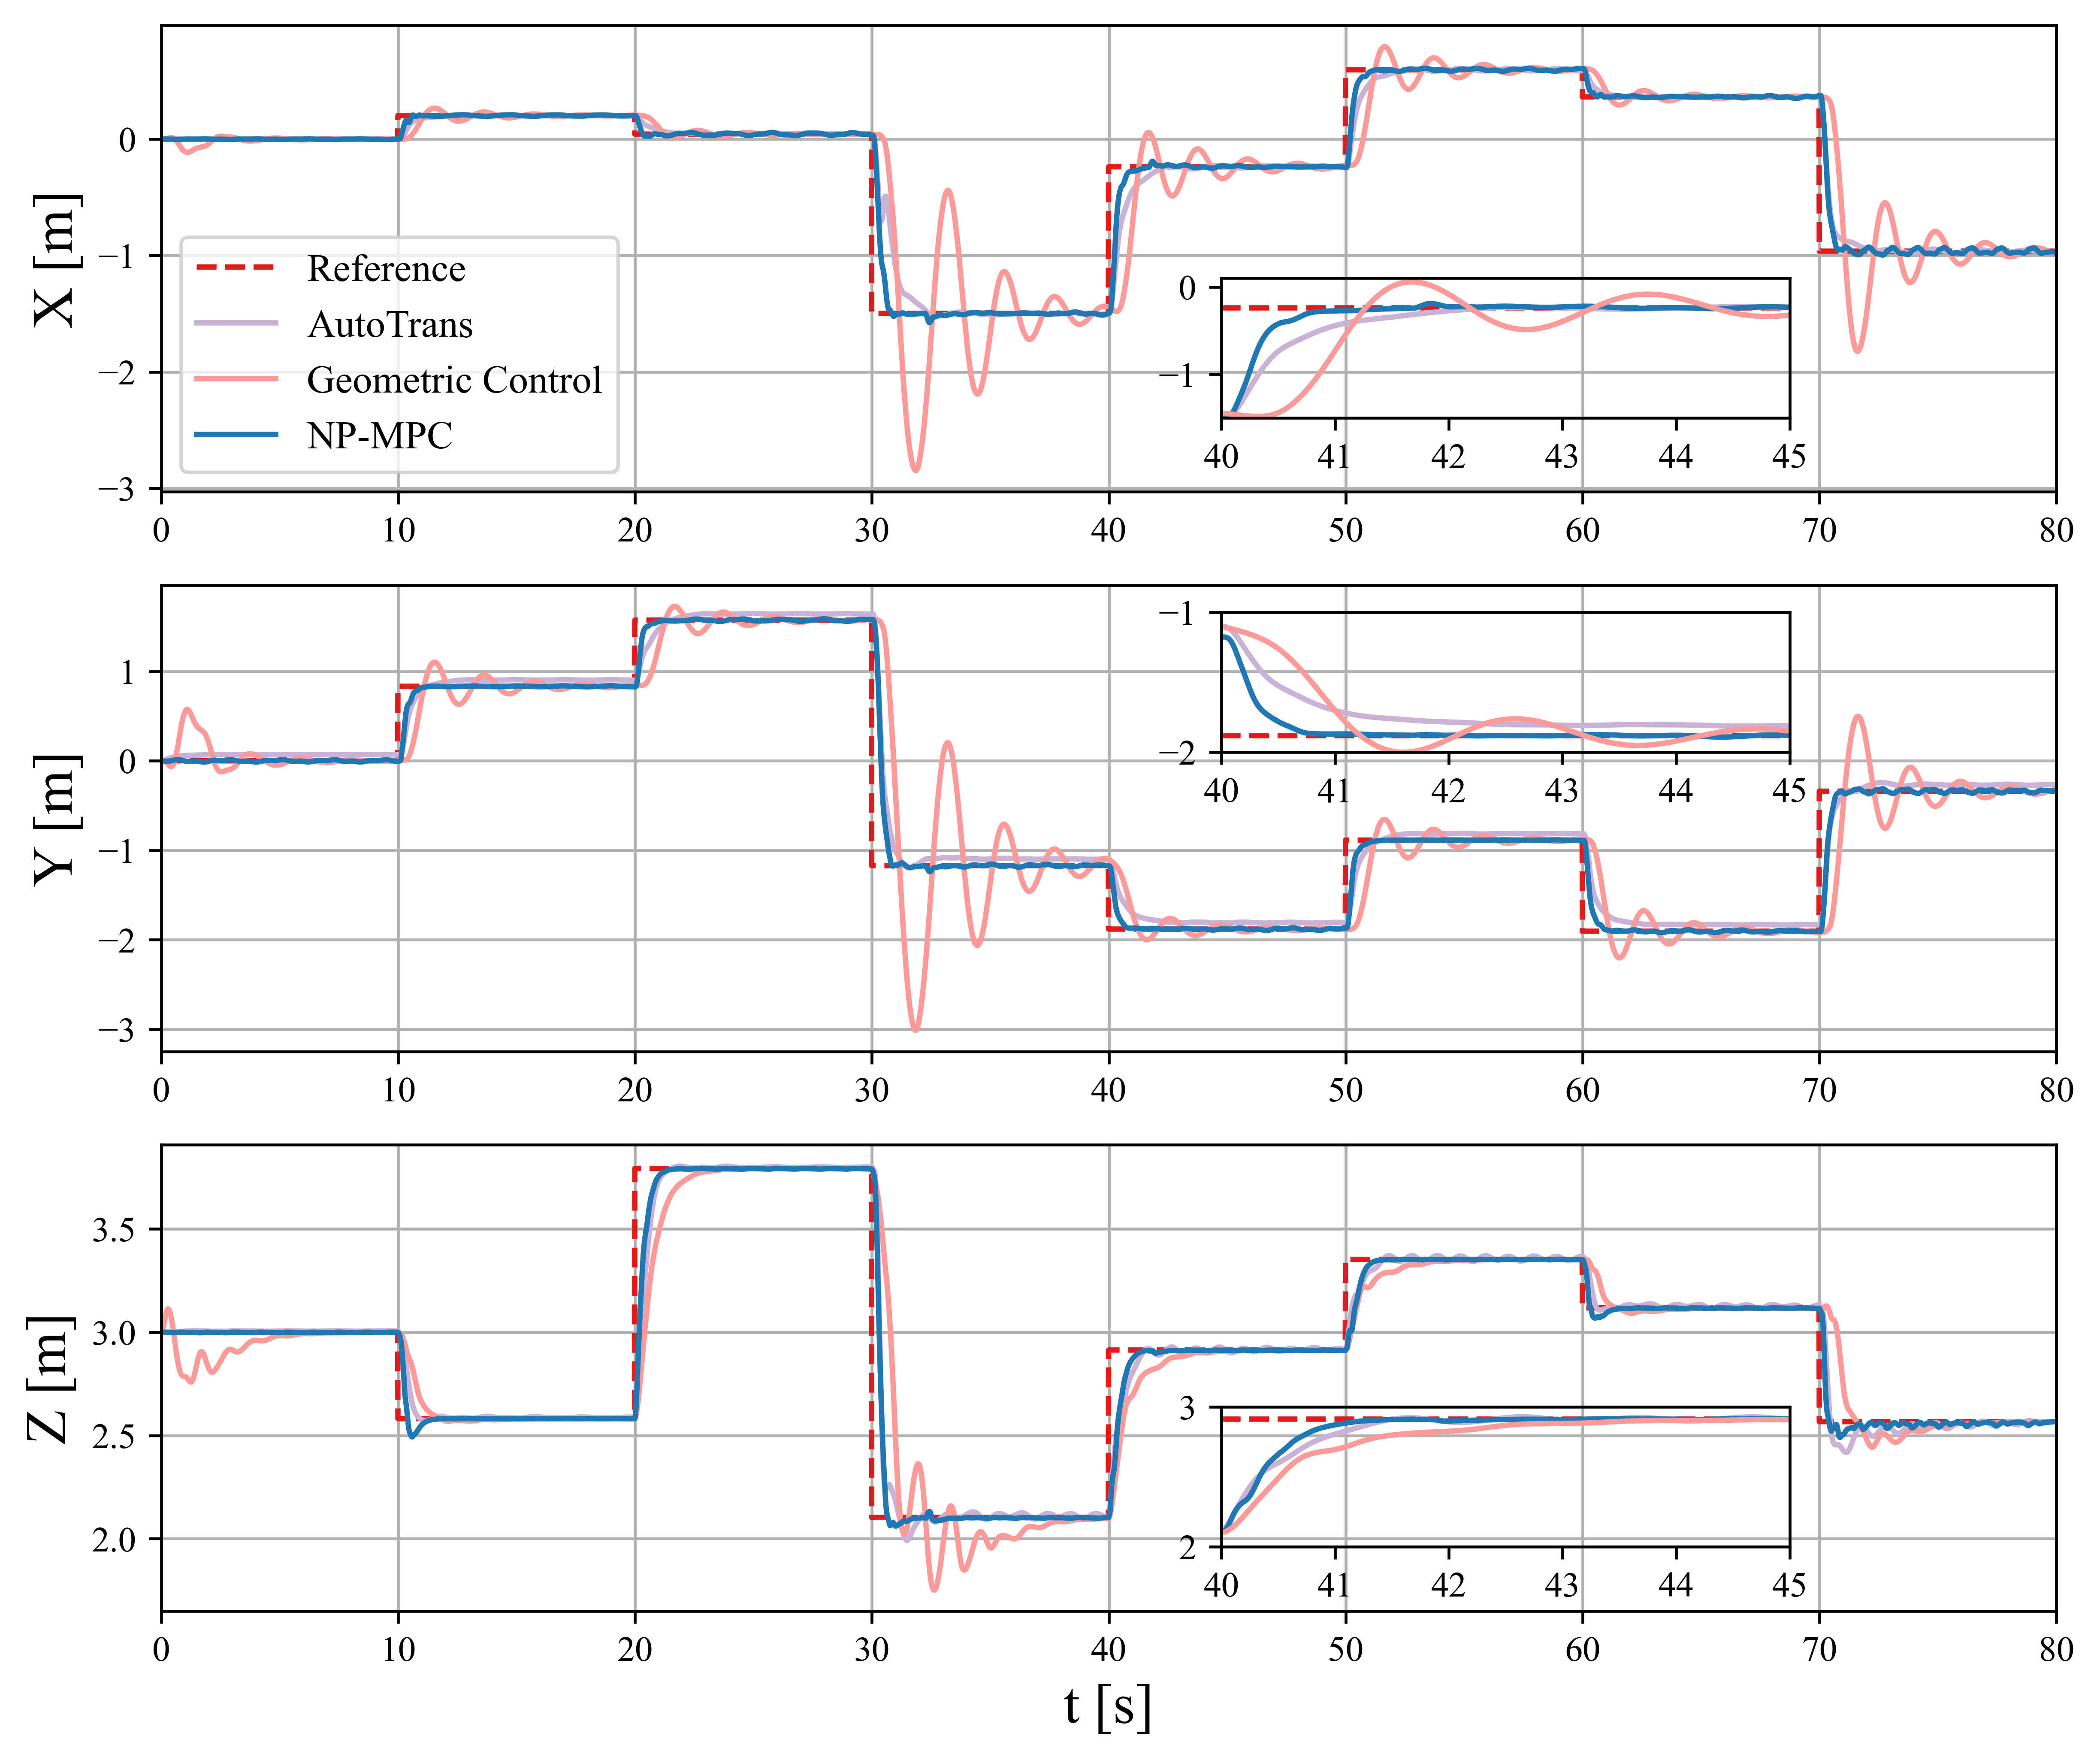
\includegraphics[width=33pc]{picture/kk/comparision.png} 
	\vspace{-0.2cm}
	\caption{无人机在随机点悬停时的仿真结果} 
	\label{comparision}
\end{figure}

在悬停仿真中,本小节随机选择了8个悬停点,每个点悬停10s。每个悬停点的吊绳与无人机之间的偏转角度$\theta$从0$^\circ$到$\text{90}^\circ$随机选取,悬停目标位置从区域$[\text{-2}, \text{2}] \times [\text{-2}, \text{2}] \times [\text{2}, \text{4}]$中随机选择,以观察无人机的稳定情况,本仿真的目的是为了验证本文所提出算法的稳定性。



在开始仿真时,载荷在空间中选取不同的初始位置,即可当作在悬停时对载荷施加了人为干扰,具体场景如图 \ref{xuanting} 所示。
无人机分别使用AutoTrans、Geometric Control 和 NP-MPC 三种算法进行了仿真验证,得到的控制曲线如图 \ref{comparision} 所示。从放大图中可以看出,NP-MPC在 1s 内可以到达设定的悬停目标点,响应速度较快,整个过程在没有超调发生的同时稳态误差趋近于 0,机身的抖振被控制在较小的范围,效果明显优于其它两种方法。

在轨迹跟踪仿真中,首先,通过多项式轨迹生成器生成了20条圆轨迹和双纽线轨迹,这些轨迹的速度和半径各不相同。随后,无人机绳系吊运系统随机选择并跟踪其中一条参考轨迹,参考轨迹的指令速度范围为0.5m/s至6m/s,且航向角参考信号在整个飞行过程中保持为零,本仿真的目的是为了验证所提出算法的轨迹跟踪精度。
\begin{figure}[hbt!]
	\centering
	\begin{subfigure}[t]{0.9\textwidth}
		\centering
		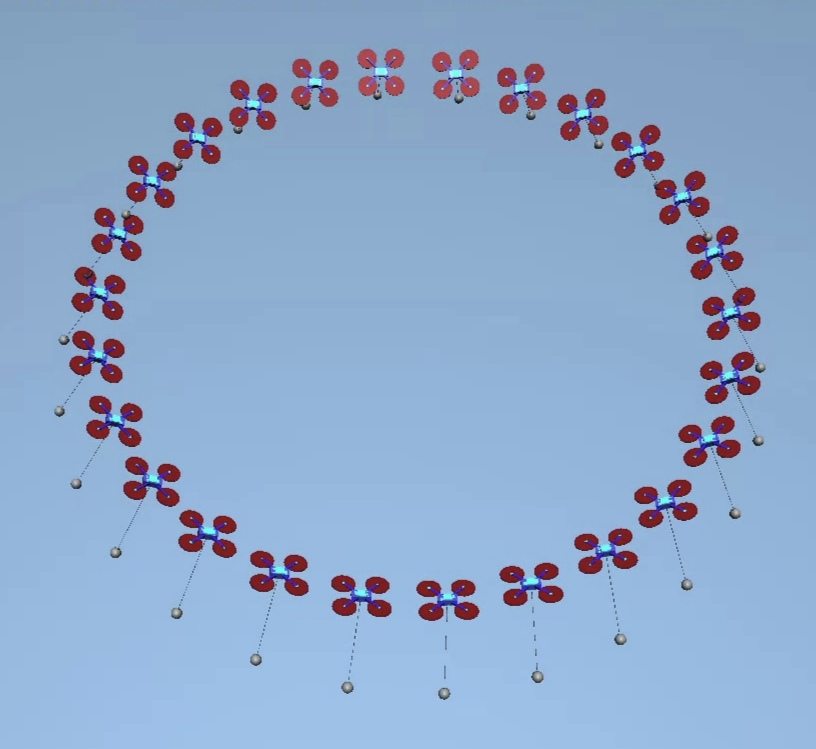
\includegraphics[width=0.98\textwidth]{picture/kk/yuan.jpg}
		\vspace{-0.2cm}
		\caption{圆轨迹}
		\label{yuana}
	\end{subfigure}\\[1.2ex] % 使得两图之间有一点间距
	\begin{subfigure}[t]{0.9\textwidth}
		\centering
		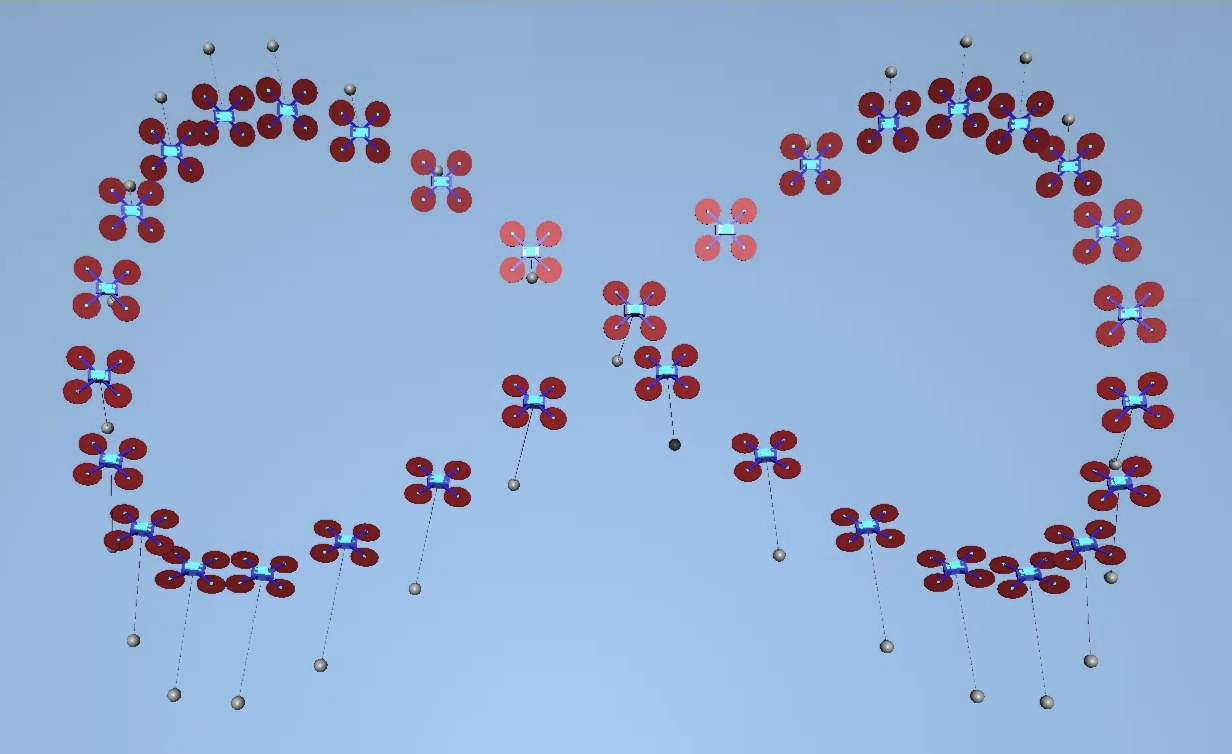
\includegraphics[width=0.98\textwidth]{picture/kk/bazi.jpg}
		\vspace{-0.2cm}
		\caption{双纽线轨迹}
		\label{bazib}
	\end{subfigure}
	\caption{无人机轨迹跟踪仿真可视化展示}
	\label{mujoco}
\end{figure}

\begin{figure}[hbt!]
	\centering
	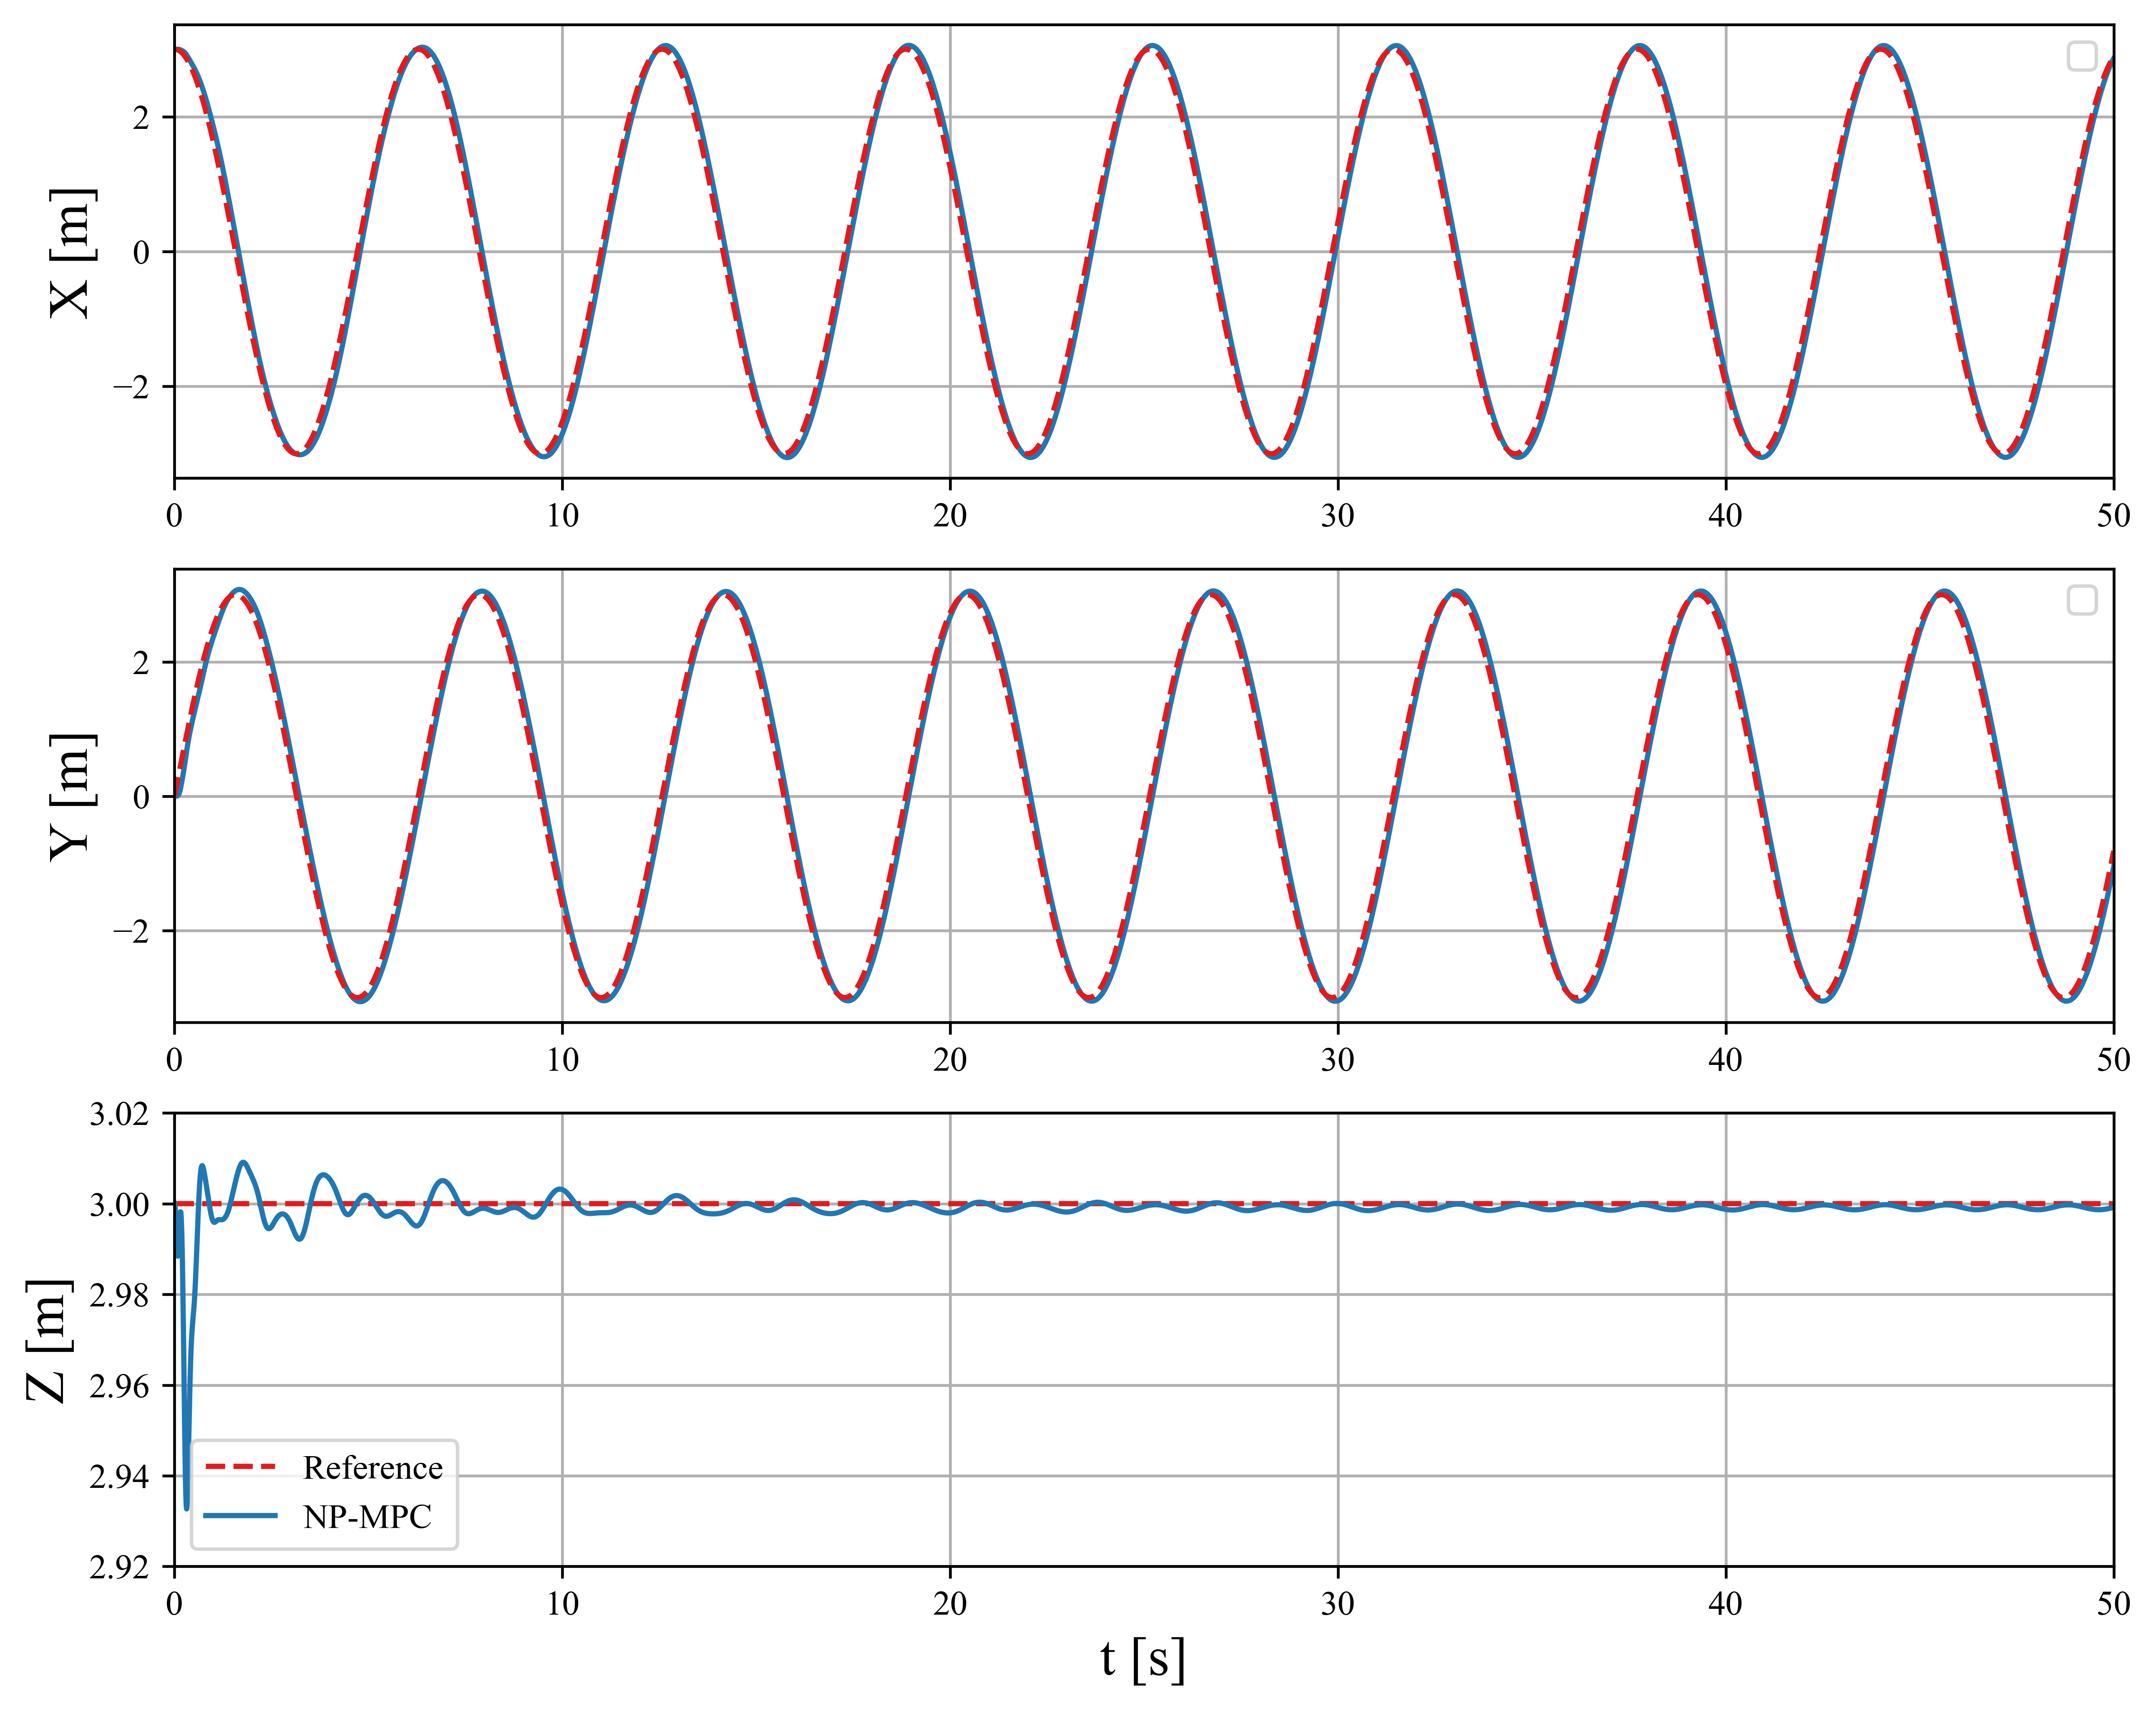
\includegraphics[width=33pc]{picture/kk/yuan.png} 
	\vspace{-0.2cm}
	\caption{无人机在圆轨迹下位置跟踪的仿真结果} 
	\label{yuan}
\end{figure}
\begin{figure}[hbt!]
	\centering
	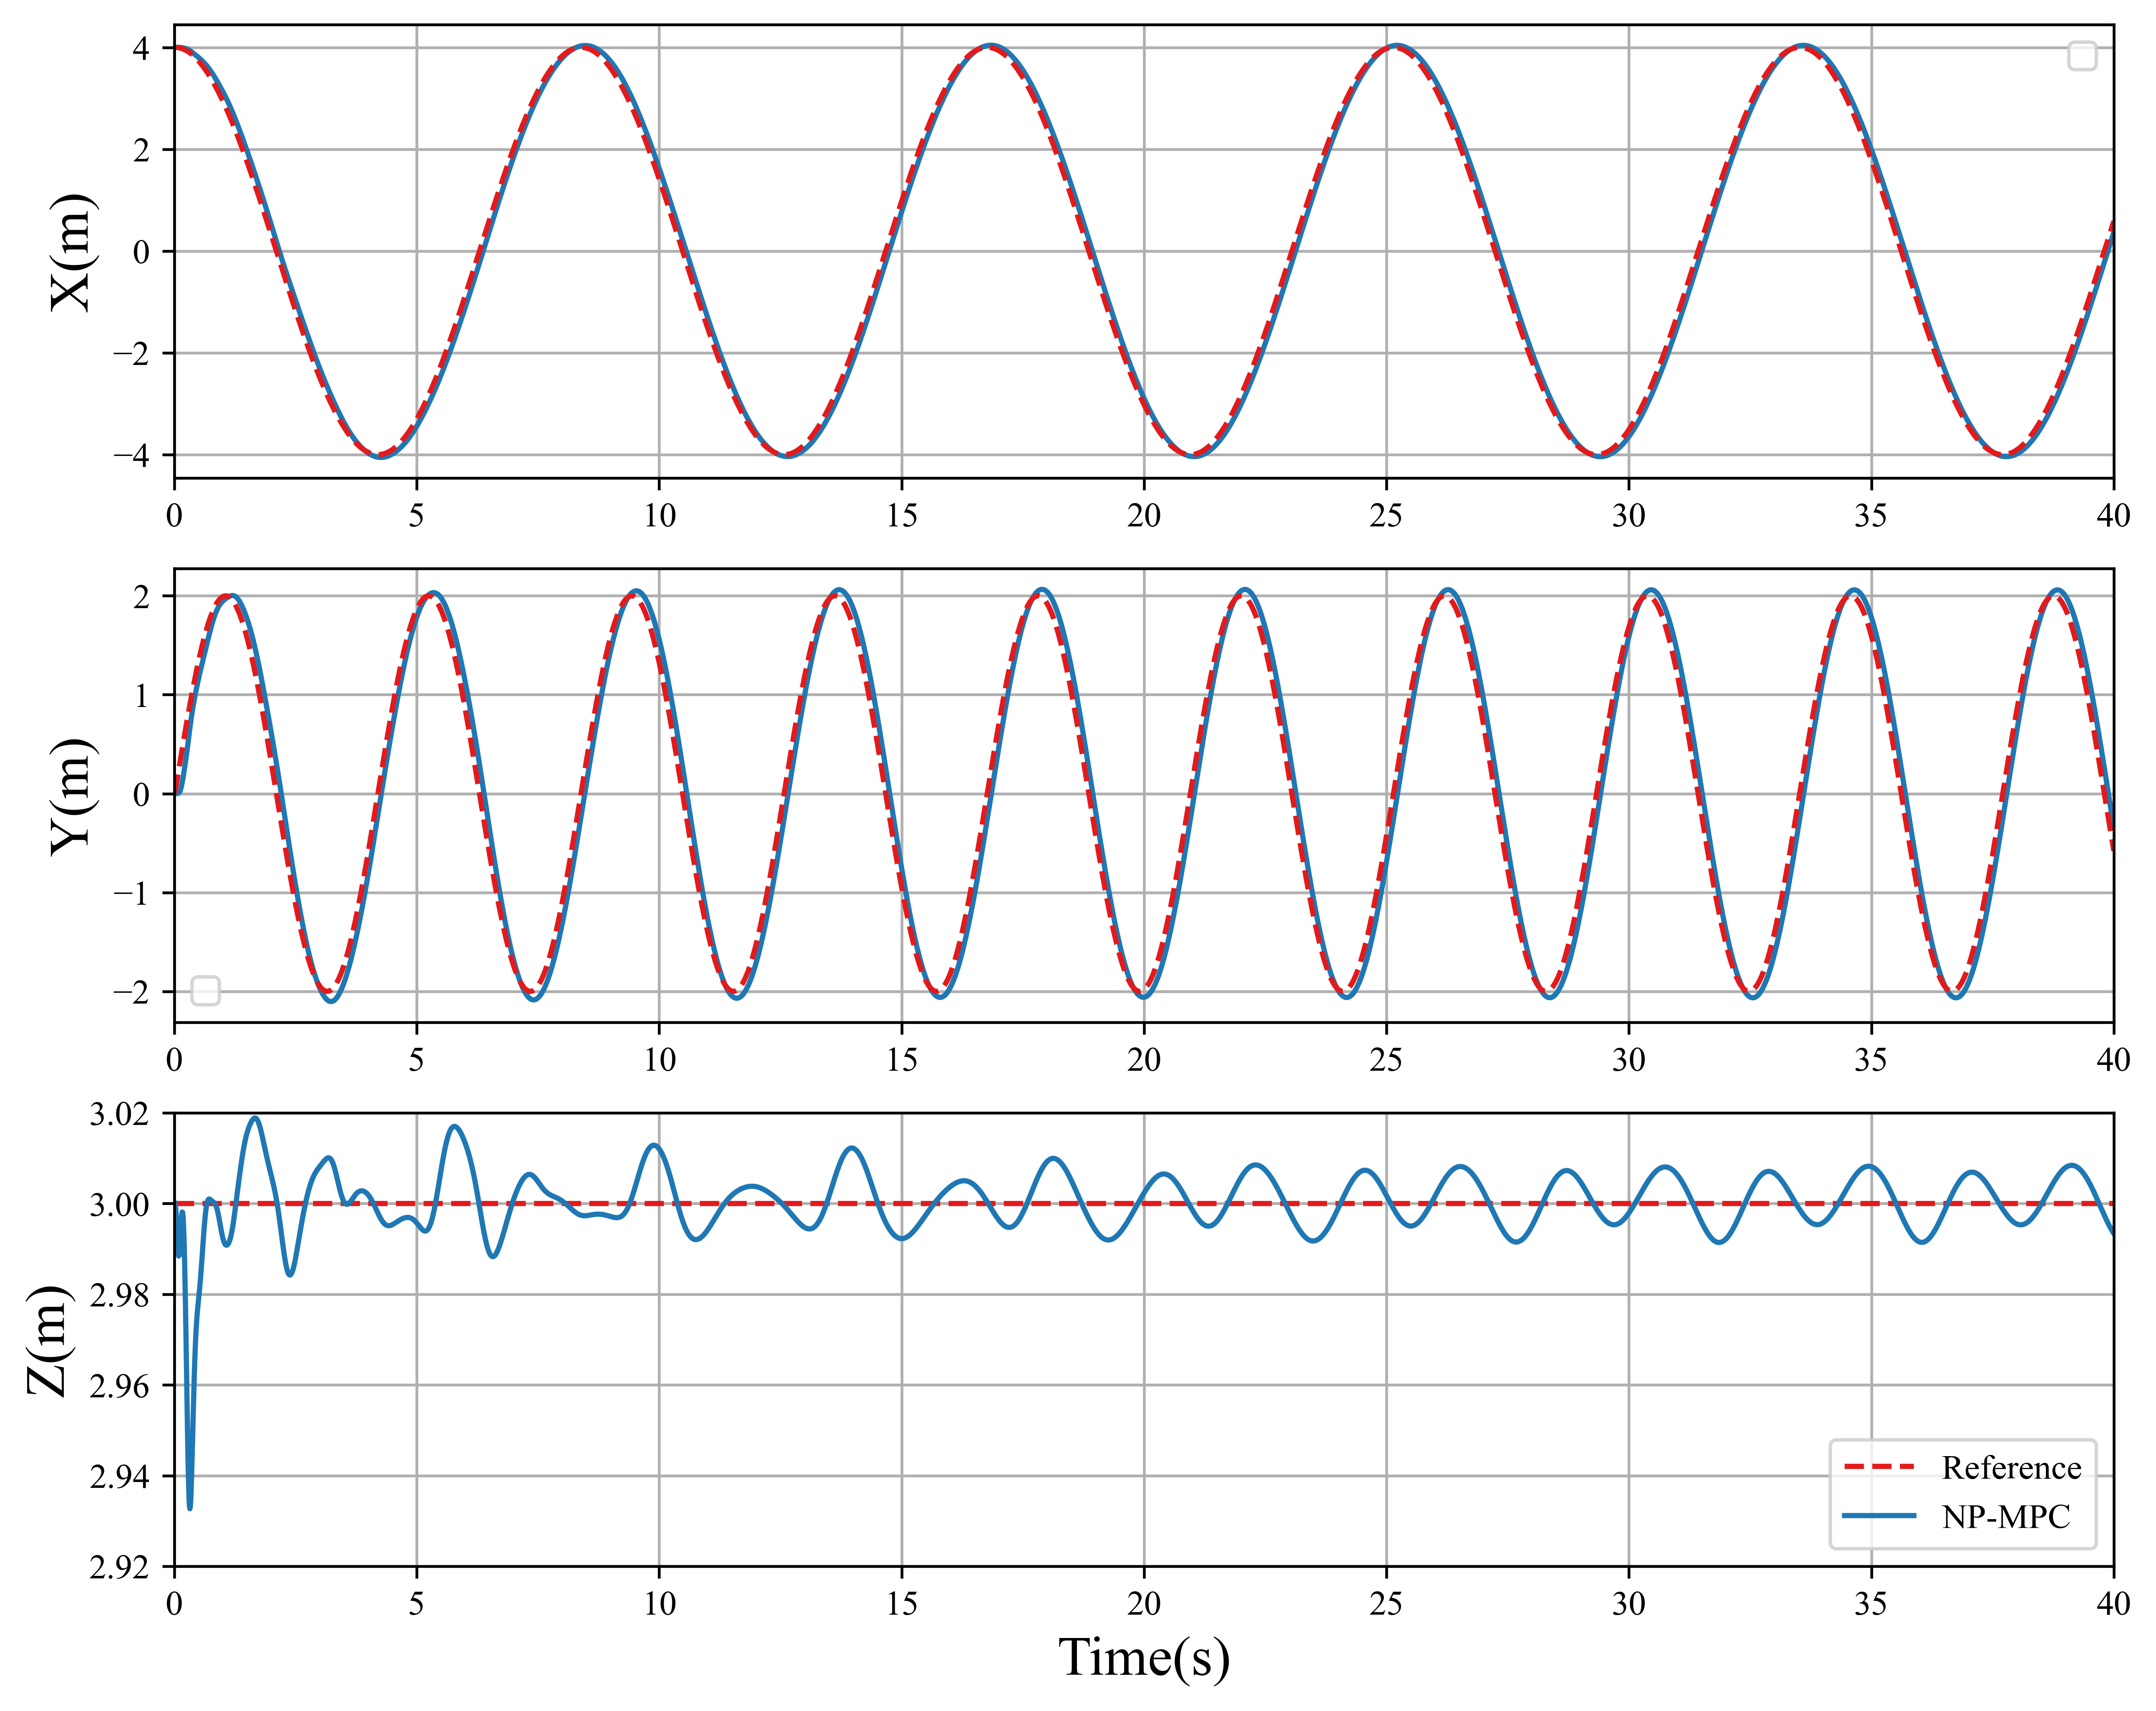
\includegraphics[width=33pc]{picture/kk/bazi.png} 
	\vspace{-0.2cm}
	\caption{无人机在双纽线轨迹下位置跟踪的仿真结果} 
	\label{bazi}
\end{figure}

\begin{table}[!ht]
    \caption{在圆和双纽线轨迹上的跟踪误差比较结果}
    \label{Table10}
    \centering
    \renewcommand\arraystretch{1.5} % 调整行间距,使表格更大
    \begin{tabular}{m{3cm}<{\centering} m{2.5cm}<{\centering} m{2.5cm}<{\centering} m{2.5cm}<{\centering} m{2.5cm}<{\centering} m{2.5cm}<{\centering}}
        \Xhline{1.pt}
        \textbf{飞行轨迹} & \textbf{最大速度 [m/s]} & \textbf{Autotrans [m]} & \textbf{Geometric Control [m]} & \textbf{NP-MPC [m]} \\
        \Xhline{1.pt}
        ~  & 1.0 & 0.0143 & 0.1721 & \textbf{0.0122} \\ 
        圆(r=2.0m)  & 2.0 & 0.0502 & 0.5728 & \textbf{0.0469} \\ 
        ~  & 3.0 & 0.0999 & 1.0565 & \textbf{0.0969} \\ \hline    
    	~ & 1.5 & 0.0305 & 0.3879 & \textbf{0.0274} \\ 
        圆(r=3.0m)  & 3.0 & 0.1108 & 1.2956 & \textbf{0.1062} \\ 
        ~  & 4.5 & 0.2269 & 2.4516 & \textbf{0.2201} \\ \hline    
        ~  & 2.0 & 0.0534 & 0.6909 & \textbf{0.0489} \\ 
        圆(r=4.0m) & 4.0 & 0.1962 & 2.3168 & \textbf{0.1898} \\ 
        ~  & 6.0 & 0.4058 & 4.5204 & \textbf{0.3980} \\ \hline    
        ~  & 0.5 & 0.0046 & 0.0422 & \textbf{0.0029} \\ 
        双纽线 (c=2.0m)  & 1.0 & 0.0147 & 0.1611 & \textbf{0.0121} \\ 
        ~  & 2.0 & \textbf{0.0433} & 0.4797 & {0.0435} \\ \hline    
        ~  & 1.0 & 0.0140 & 0.1691 & \textbf{0.0117} \\ 
        双纽线 (c=4.0m)  & 2.0 & 0.0531 & 0.6473 & \textbf{0.0487} \\ 
        ~ &  4.0 & 0.1762 & 2.0703 & \textbf{0.1757} \\ \hline    
        ~ &  1.5 & 0.0297 & 0.3814 & \textbf{0.0265} \\ 
        双纽线 (c=6.0m) & 3.0 & 0.1174 & 1.4638 & \textbf{0.1103} \\ 
         ~ & 6.0 & 0.4183 & 3.5491 & \textbf{0.4007} \\ \hline        \Xhline{1.pt}
    \end{tabular}
\end{table}


在开始仿真时,无人机默认静止在飞行轨迹的起始点上,在MuJoCo中用外部可视化工具可视化了圆轨迹和双纽线轨迹,具体场景如图 \ref{mujoco} 所示。图 \ref{yuan} 和图 \ref{bazi} 分别显示了无人机在跟踪圆轨迹和双纽线轨迹位置回路跟踪结果。可以看出在激烈飞行中,无人机的位置回路跟踪效果仍然十分优异, 在NP-MPC算法的作用下,可以很快收敛到期望轨迹,并在激烈飞行时也确保了轨迹跟踪的实时性。
在不同速度和轨迹条件下,NP-MPC的跟踪性能也通过试验与AutoTrans和Geometric Control方法进行了对比分析。仿真结果如表 \ref{Table10} 所示,NP-MPC和AutoTrans在所有仿真案例中的轨迹跟踪性能均优于Geometric Control。在激烈的飞行条件下,NP-MPC能够实现与AutoTrans相当的性能。不同之处在于,AutoTrans依赖于有效载荷的先验信息,例如载荷质量和系绳长度等参数,而NP-MPC无需依赖这些信息即可稳定运行。这是因为NP-MPC将外力建模为一个动态系统,从而能够在四旋翼状态变化时实时预测外力,其它传统的方法在外力估计的过程中则可能会存在延迟。

\subsection{多无人机吊运仿真验证}
在多无人机吊运仿真仿真中,三架无人机和有效载荷的质量分别为0.75kg和1.5kg,无人机与有效载荷之间的吊绳长度为2m,其它设置与单无人机吊运仿真相同。


通过轨迹跟踪仿真对设计的 Autotune-MPC 算法进行了验证。首先,通过多项式轨迹生成器生成了载荷的期望轨迹和三架无人机的期望轨迹,并使用 传统 MPC 和 Autotune-MPC 在仿真引擎中分别进行跟踪。仿真结果如下图所示:
\begin{figure}[H]
	\centering
	% 第一行的两张图
	\begin{subfigure}[b]{0.48\textwidth}
		\centering
		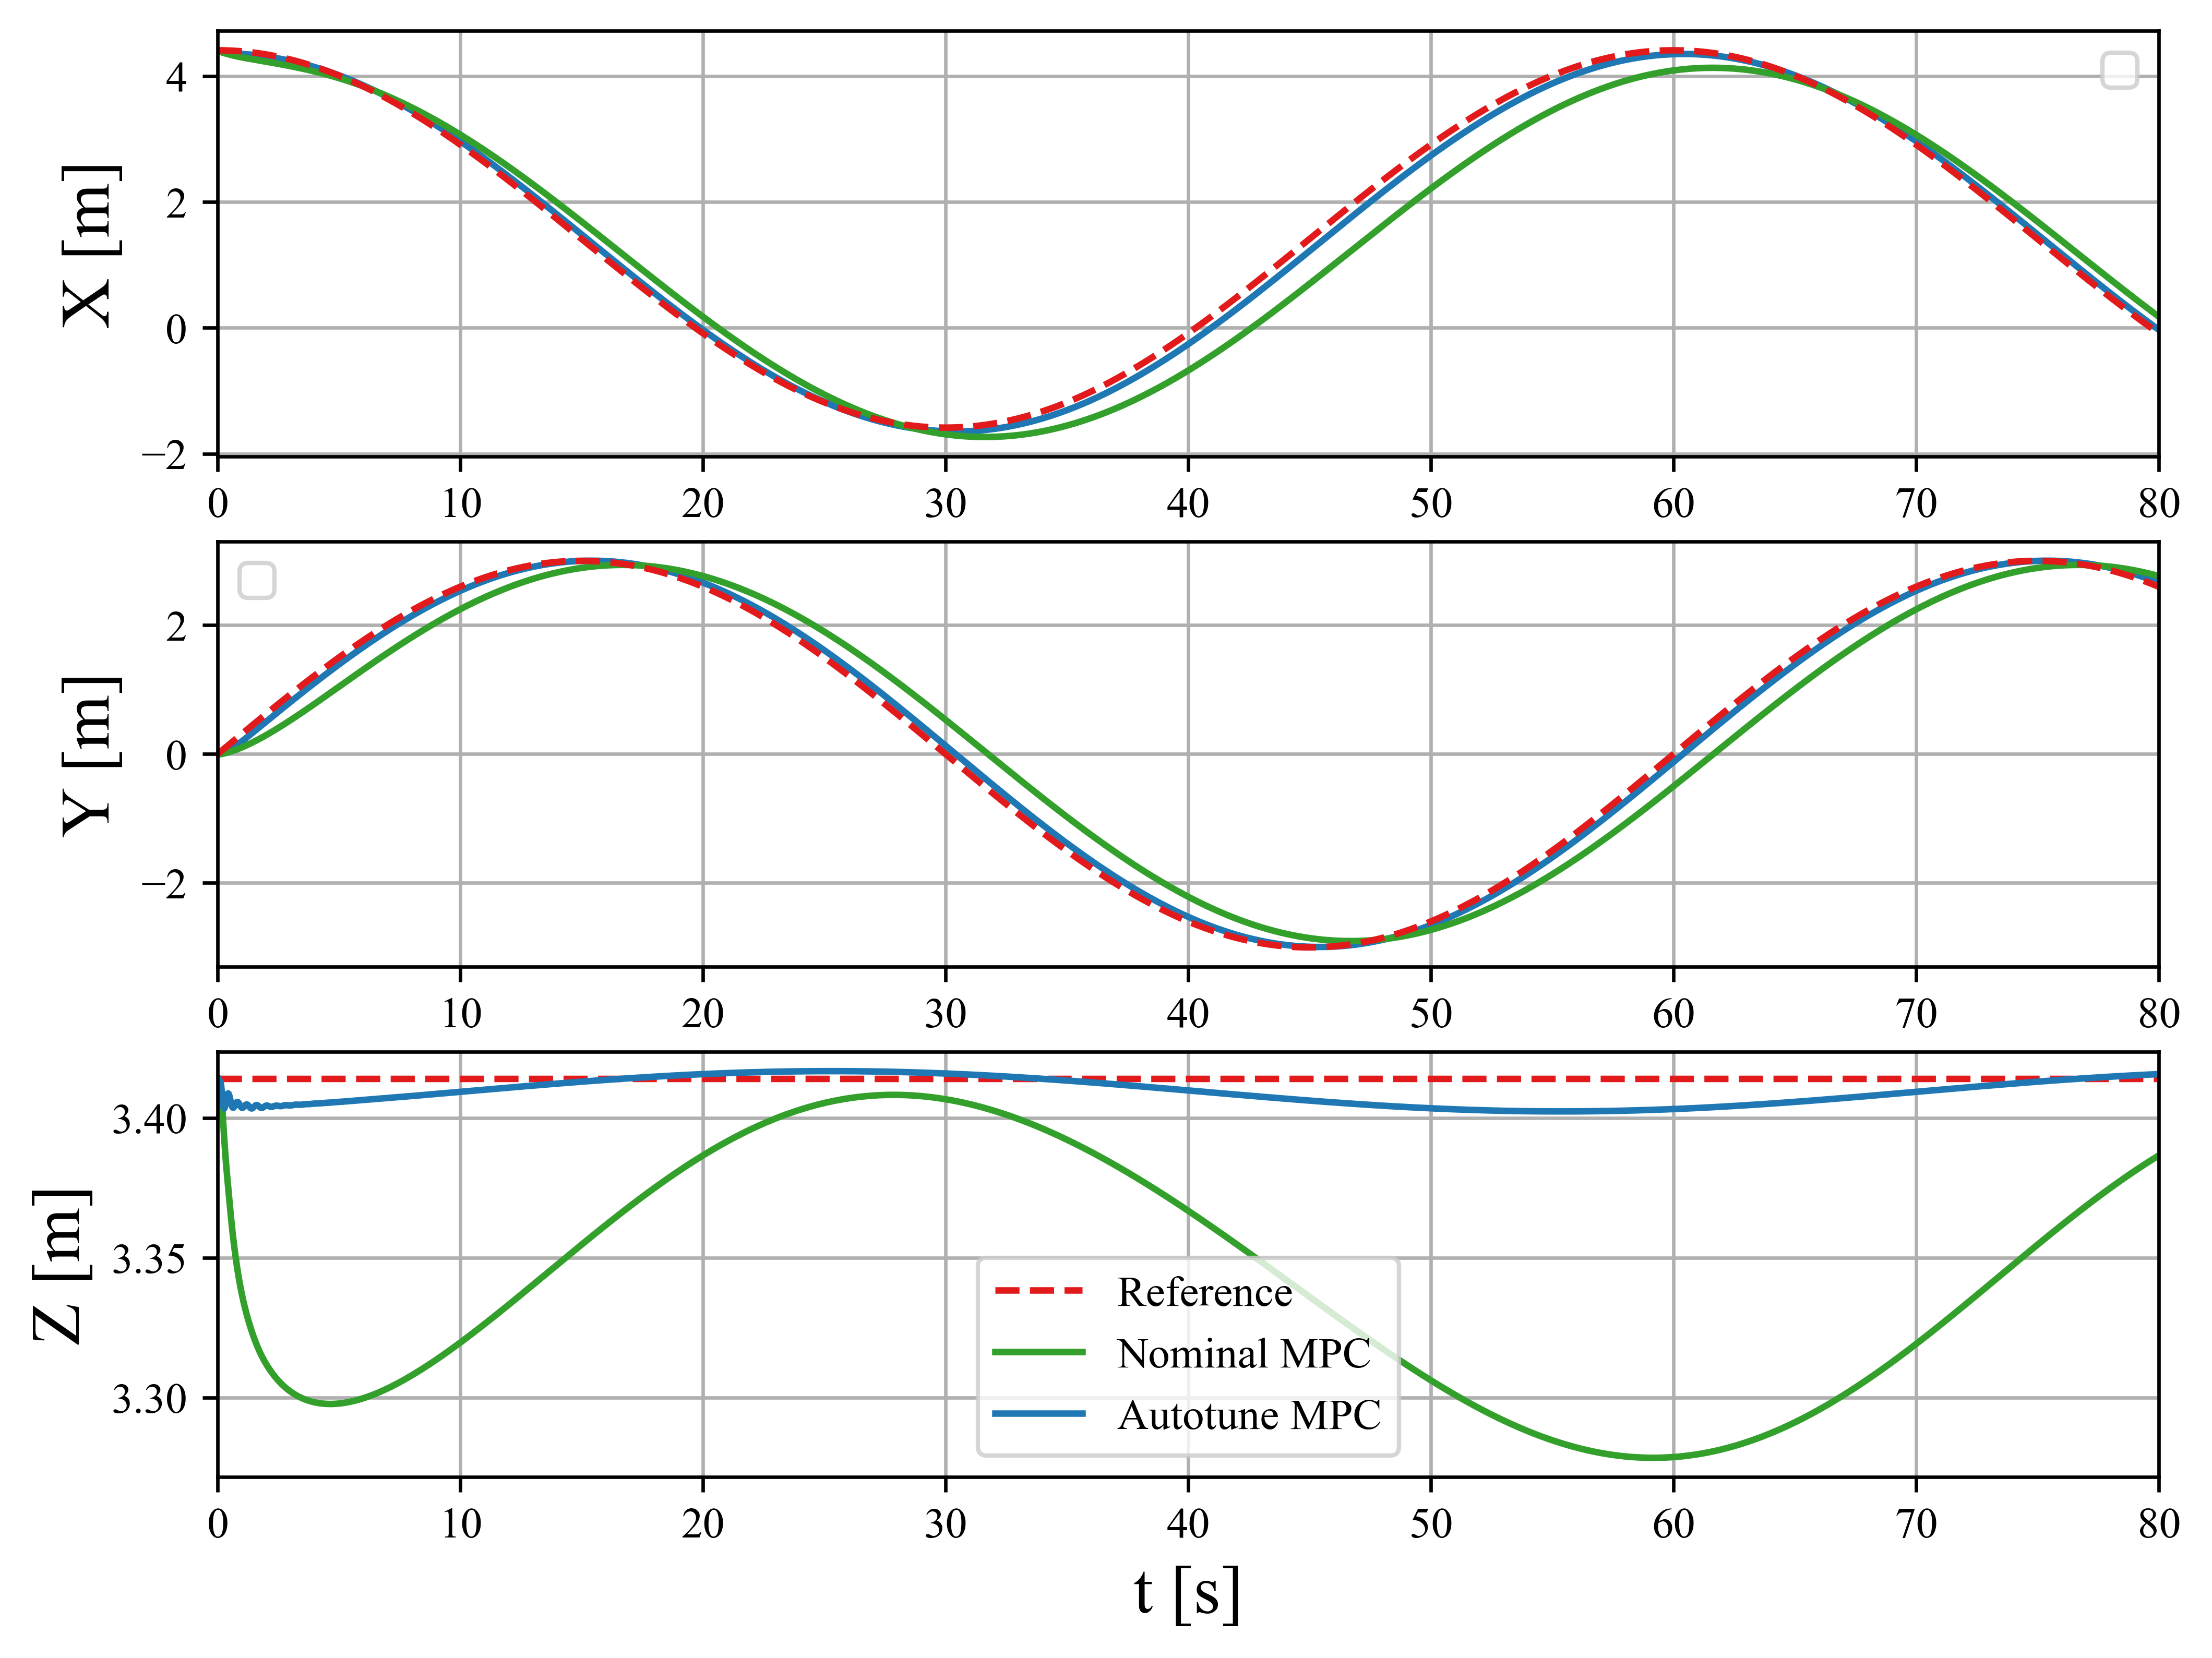
\includegraphics[width=\textwidth]{picture/kk2/quadrotor0.png}
		\caption{无人机1}
		\label{quadrotor0}
	\end{subfigure}
	\hfill
	\begin{subfigure}[b]{0.48\textwidth}
		\centering
		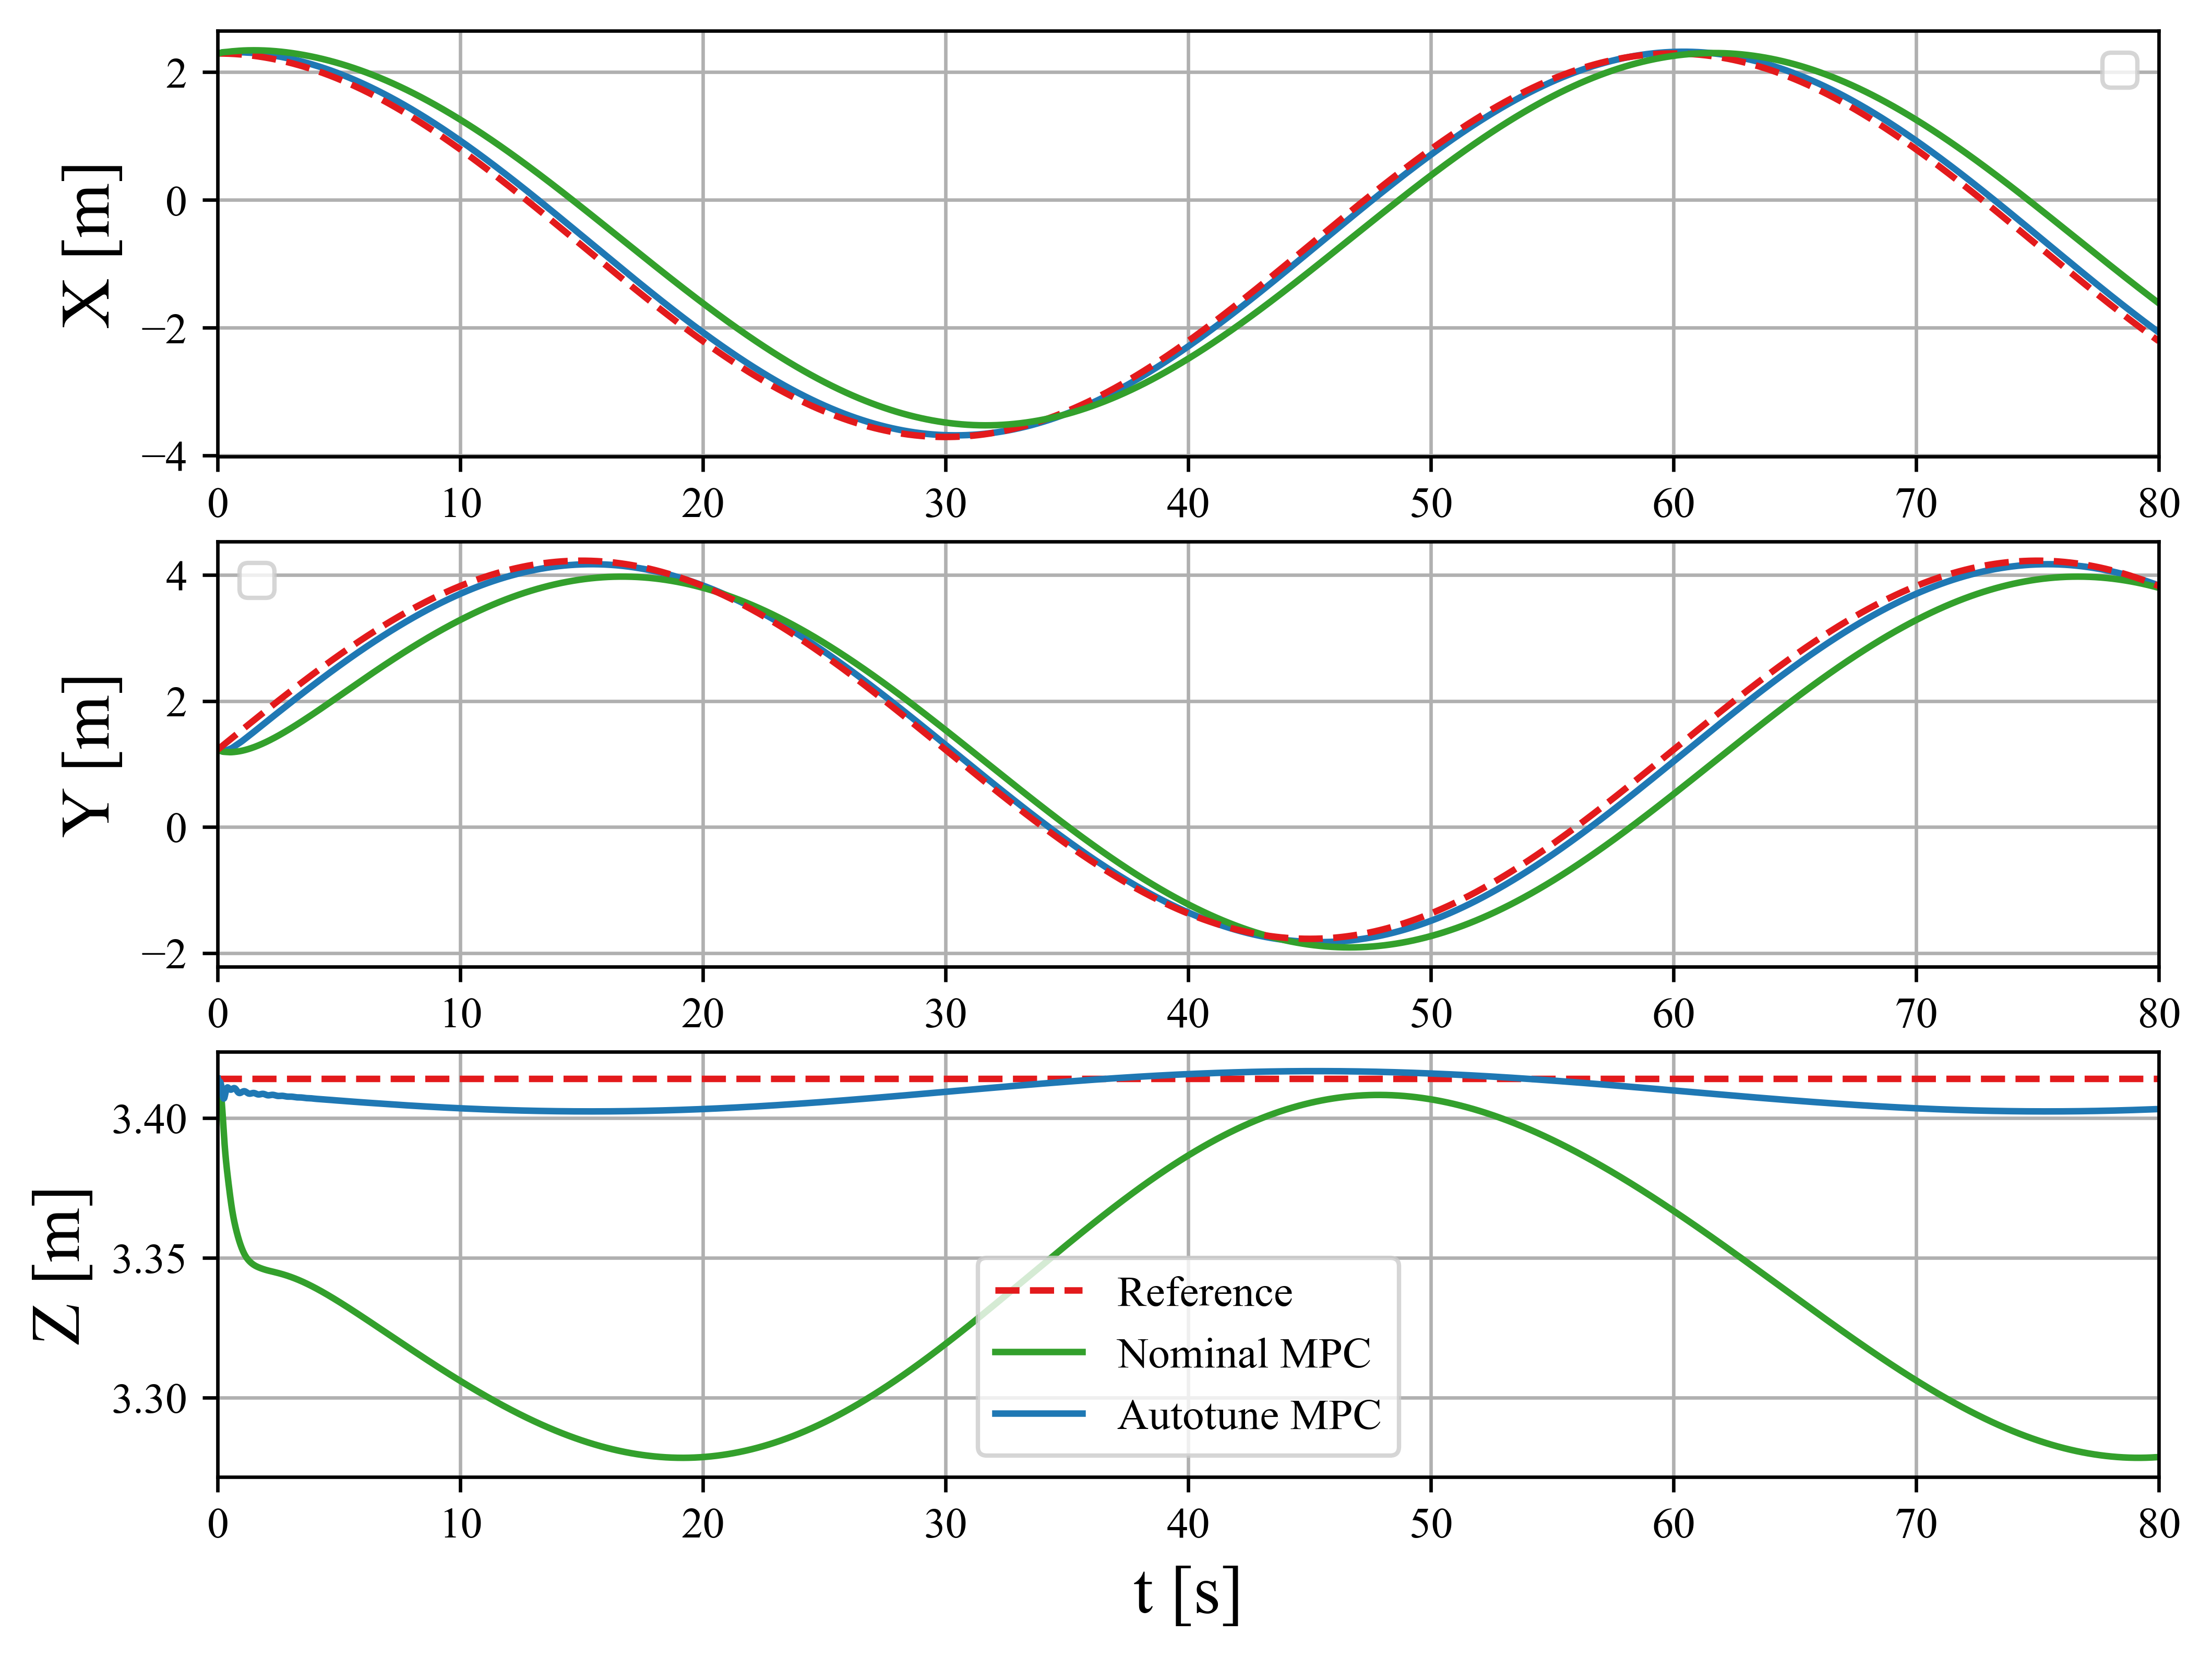
\includegraphics[width=\textwidth]{picture/kk2/quadrotor1.png}
		\caption{无人机2}
		\label{quadrotor1}
	\end{subfigure}
	
	\vspace{0.5cm} % 调整两行之间的垂直间距
	
	% 第二行的两张图
	\begin{subfigure}[b]{0.48\textwidth}
		\centering
		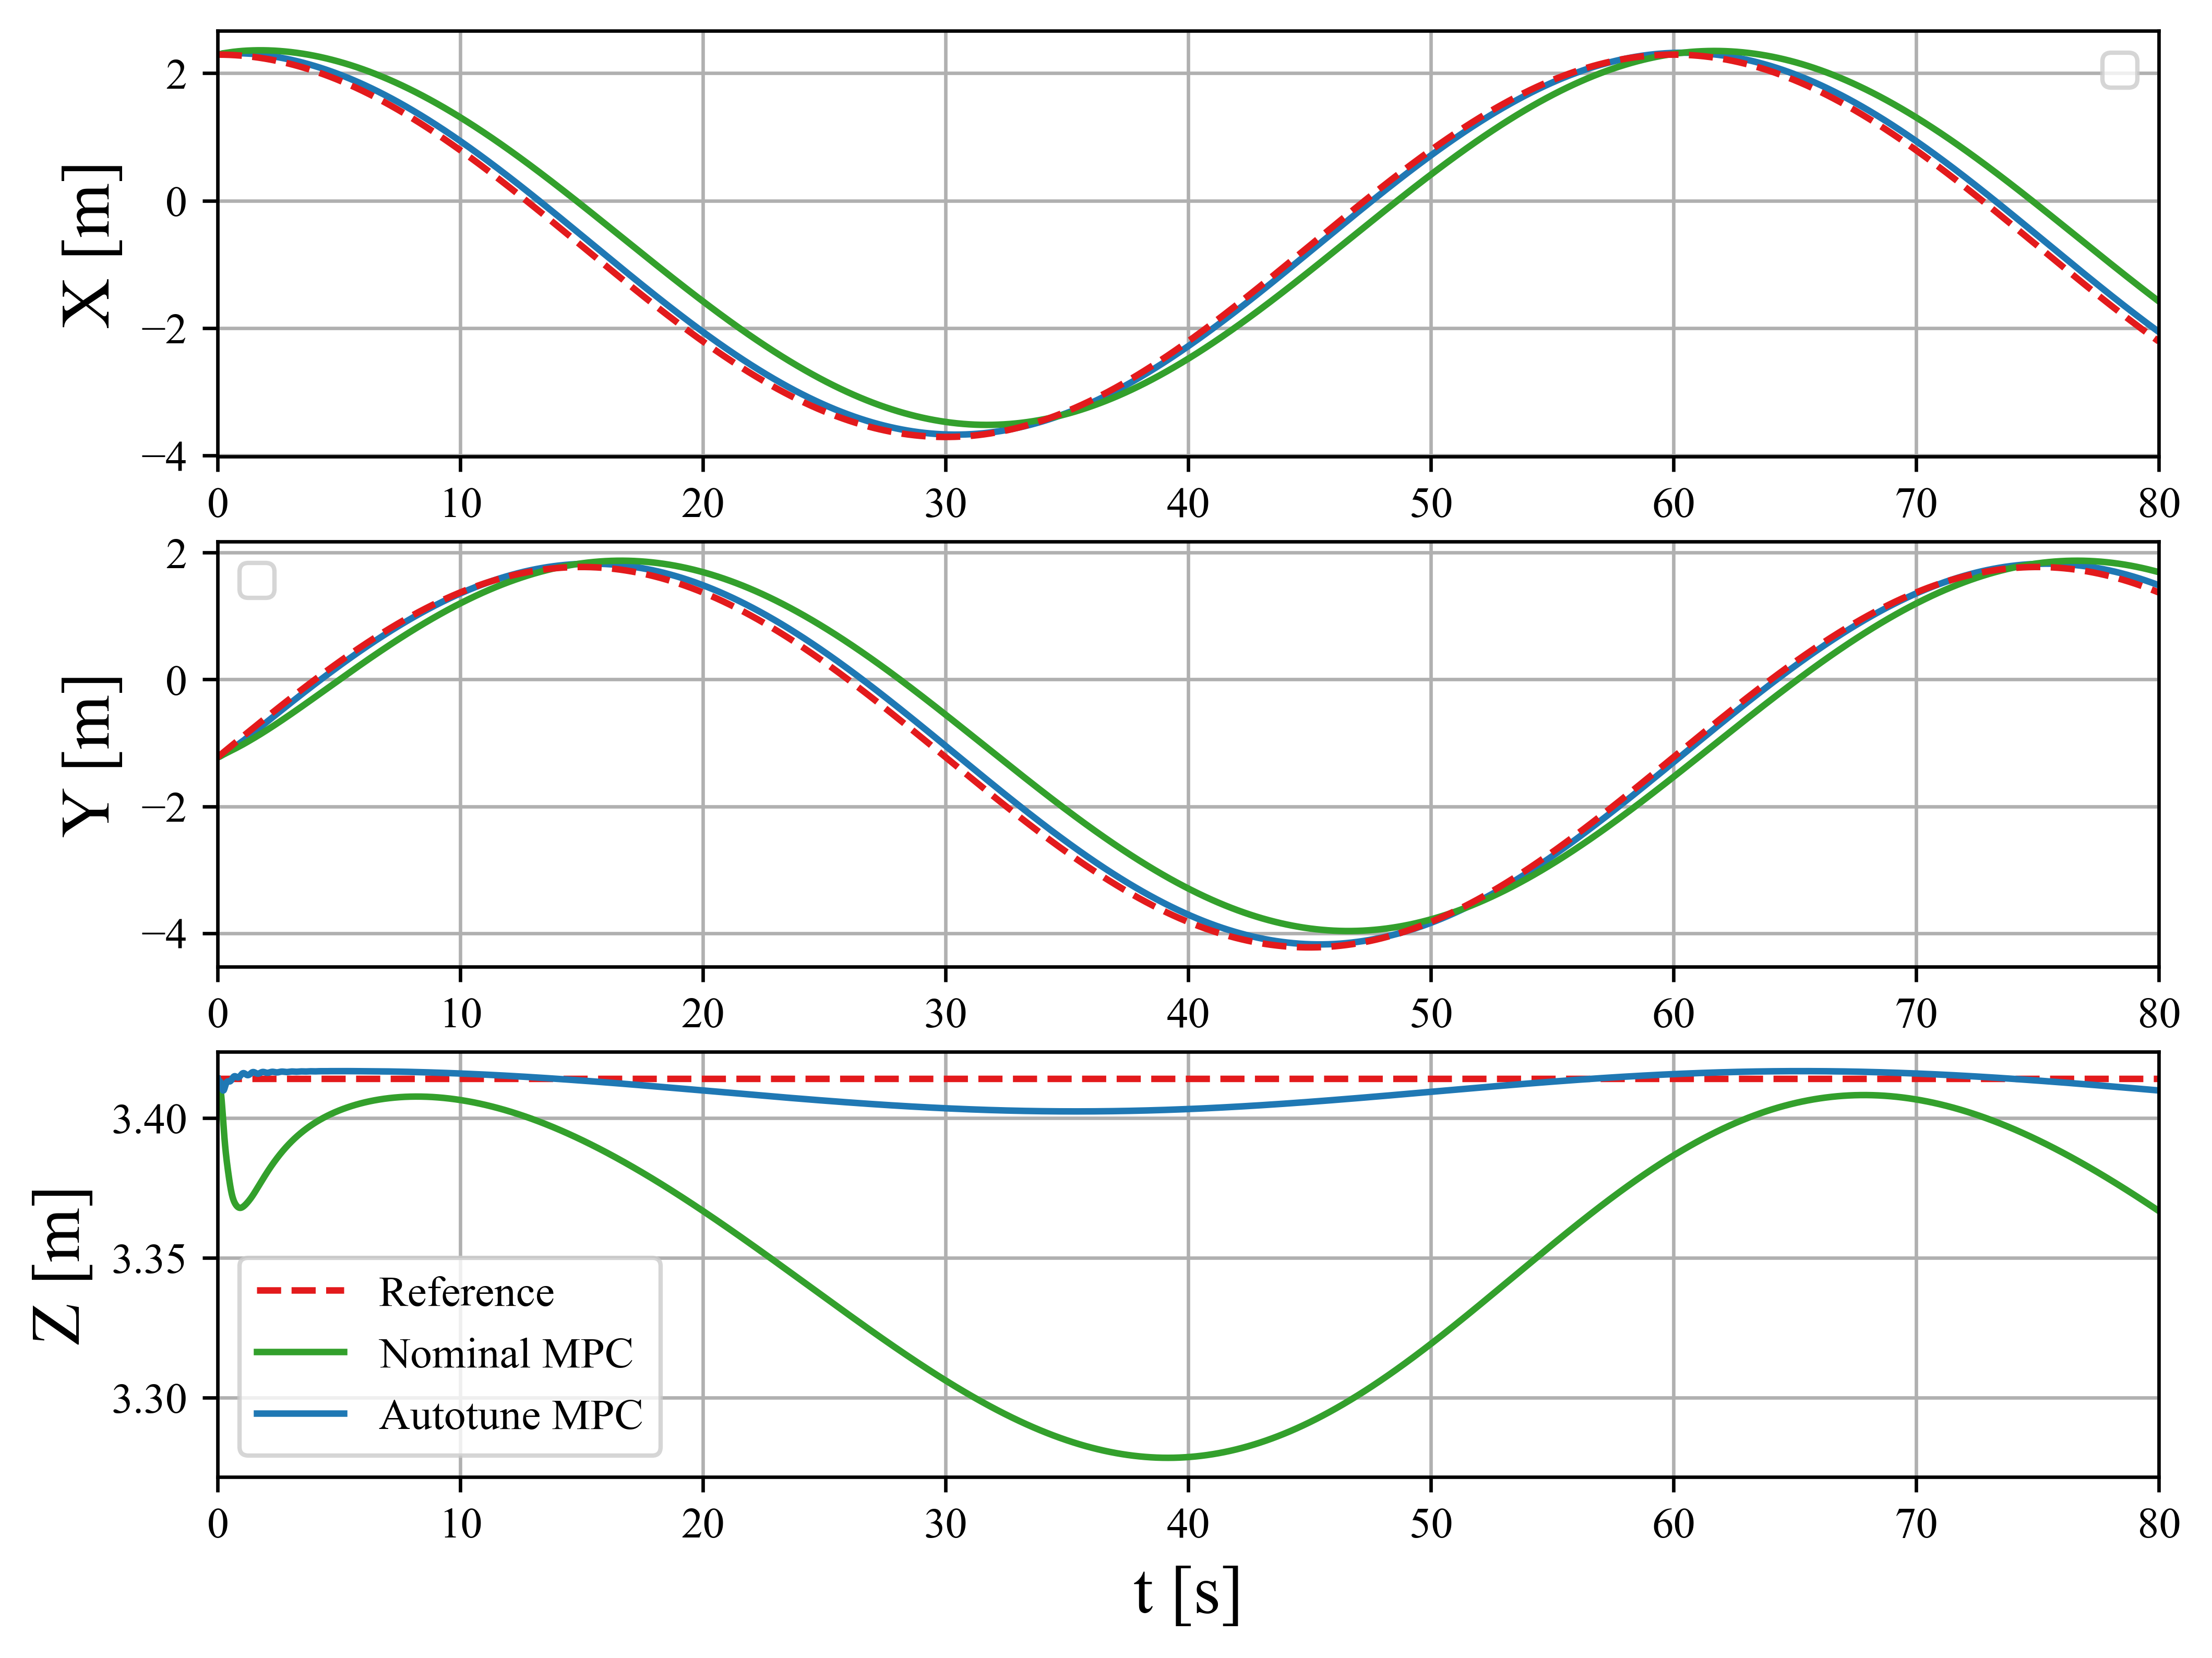
\includegraphics[width=\textwidth]{picture/kk2/quadrotor2.png}
		\caption{无人机3}
		\label{quadrotor2}
	\end{subfigure}
	\hfill
	\begin{subfigure}[b]{0.48\textwidth}
		\centering
		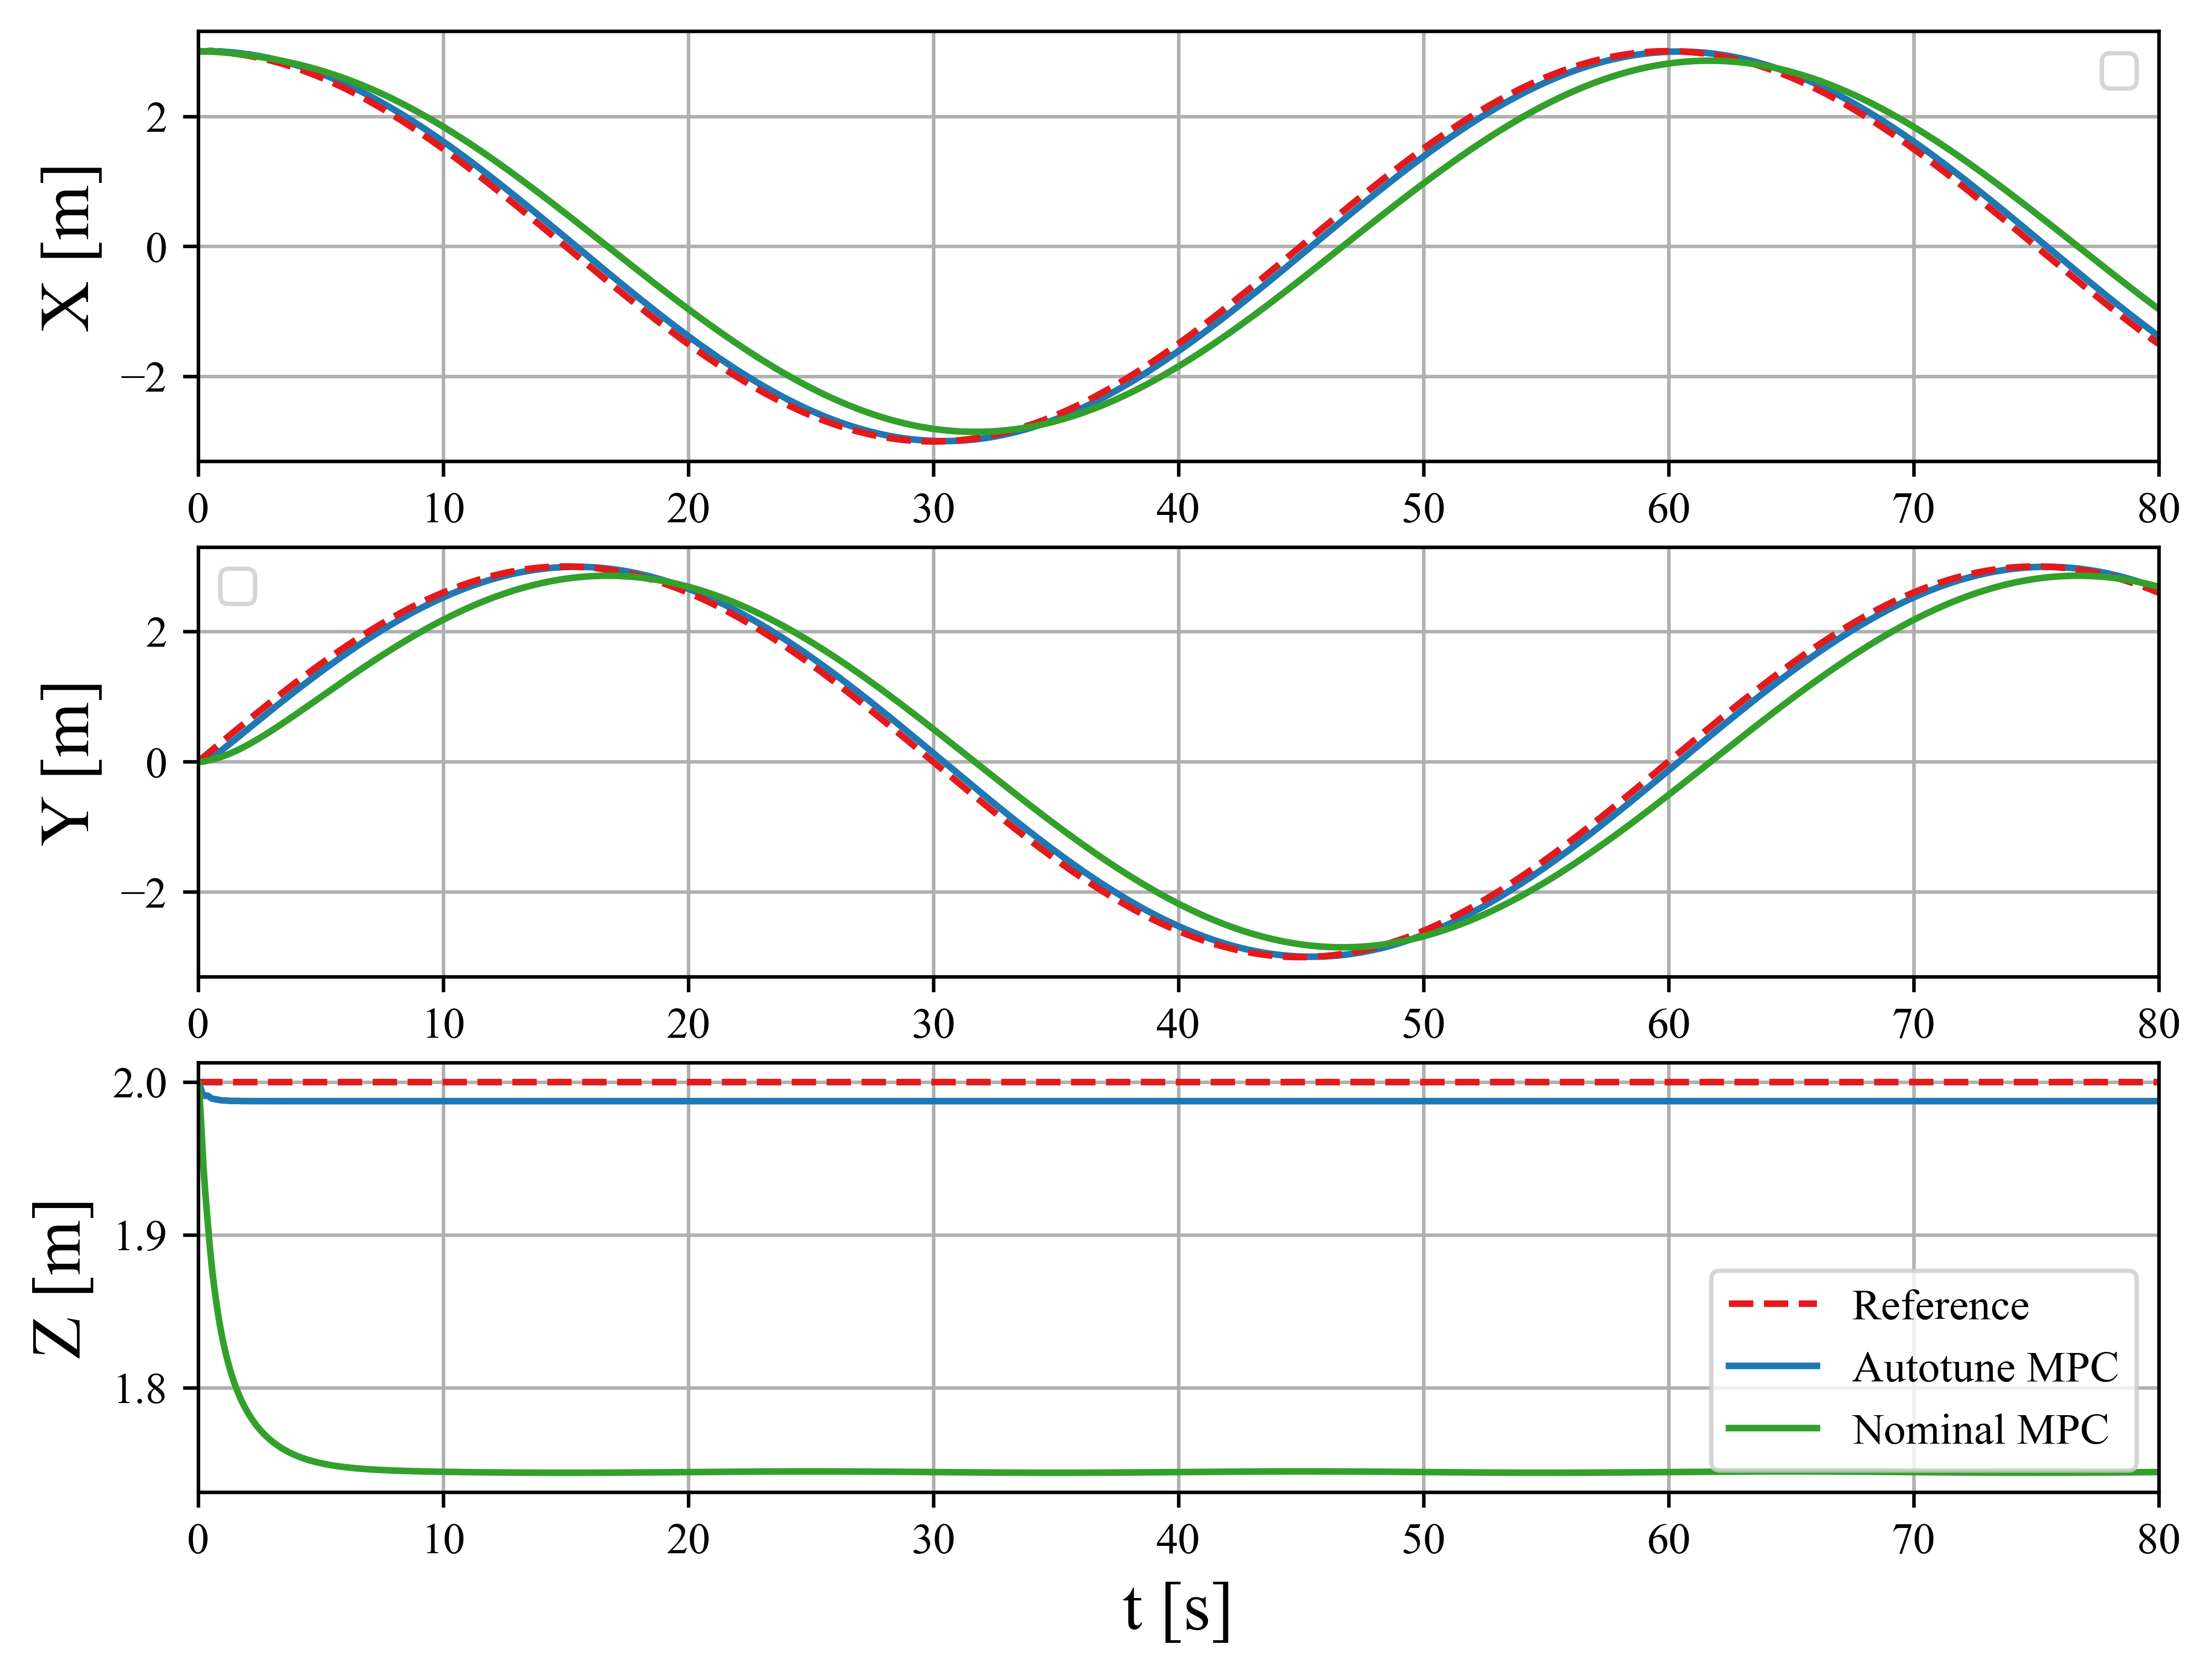
\includegraphics[width=\textwidth]{picture/kk2/load.png}
		\caption{载荷}
		\label{load}
	\end{subfigure}
	
	\caption{多无人机和载荷位置跟踪的仿真结果}
	\label{tt}
\end{figure}

\autoref{tt} 显示了多无人机和载荷对于期望位置和期望姿态的跟踪效果, Autotune-MPC  算法在传统的MPC算法的基础上对无人机和载荷中的超参数进行了实时的更新调整,参数更加准确,控制效率和精度更高,算法的跟踪效果有了明显的提升。多无人机和载荷在各个方向上的跟踪误差如\autoref{ex} 到\autoref{ez} 所示,在 Autotune-MPC 算法中,提升最明显的是载荷的跟踪精度,这是由于载荷接收到了来自各个无人机和自身的灵敏度,并通过梯度下降的分布式策略对超参数进行了调整,从而确保了载荷能够沿预定轨迹精确运动,显著提升了控制精度。\autoref{combined3D} 显示了三维空间下的跟踪效果图。



\begin{figure}[H]
	\centering
	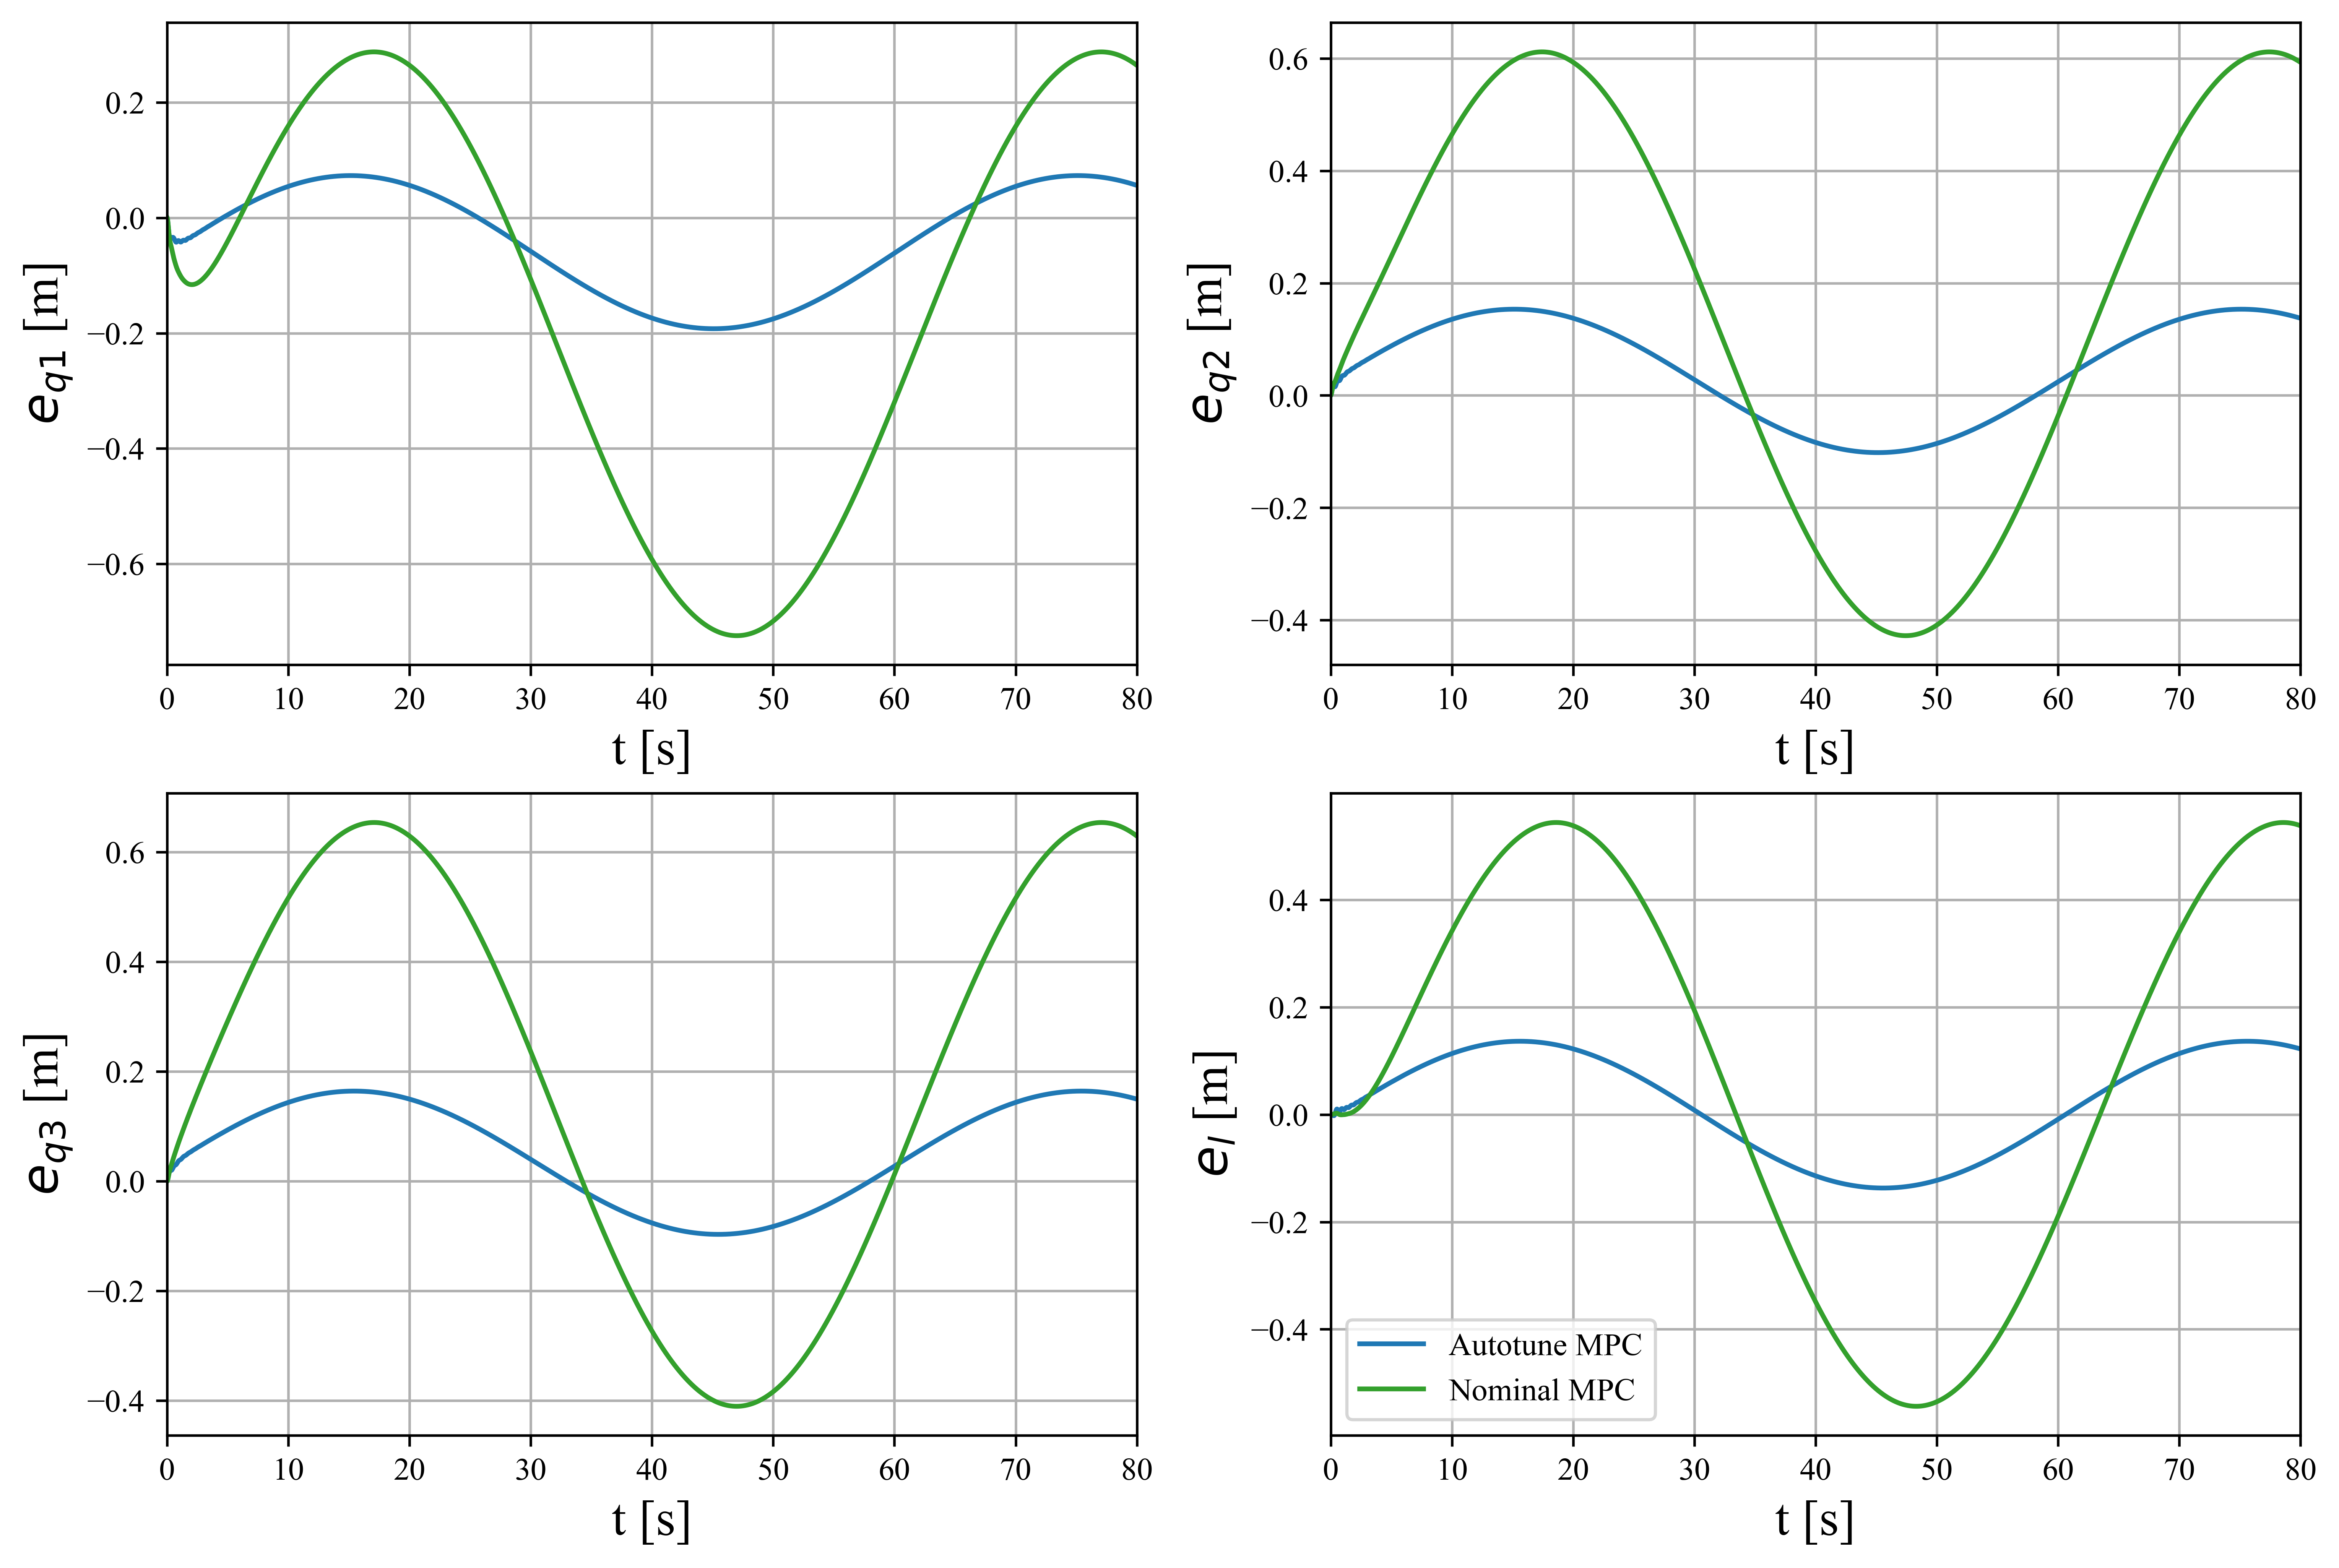
\includegraphics[width=38pc]{picture/kk2/ex.png} 
	\caption{多无人机和载荷X轴上的跟踪误差} 
	\label{ex}
\end{figure}

\begin{figure}[H]
	\centering
	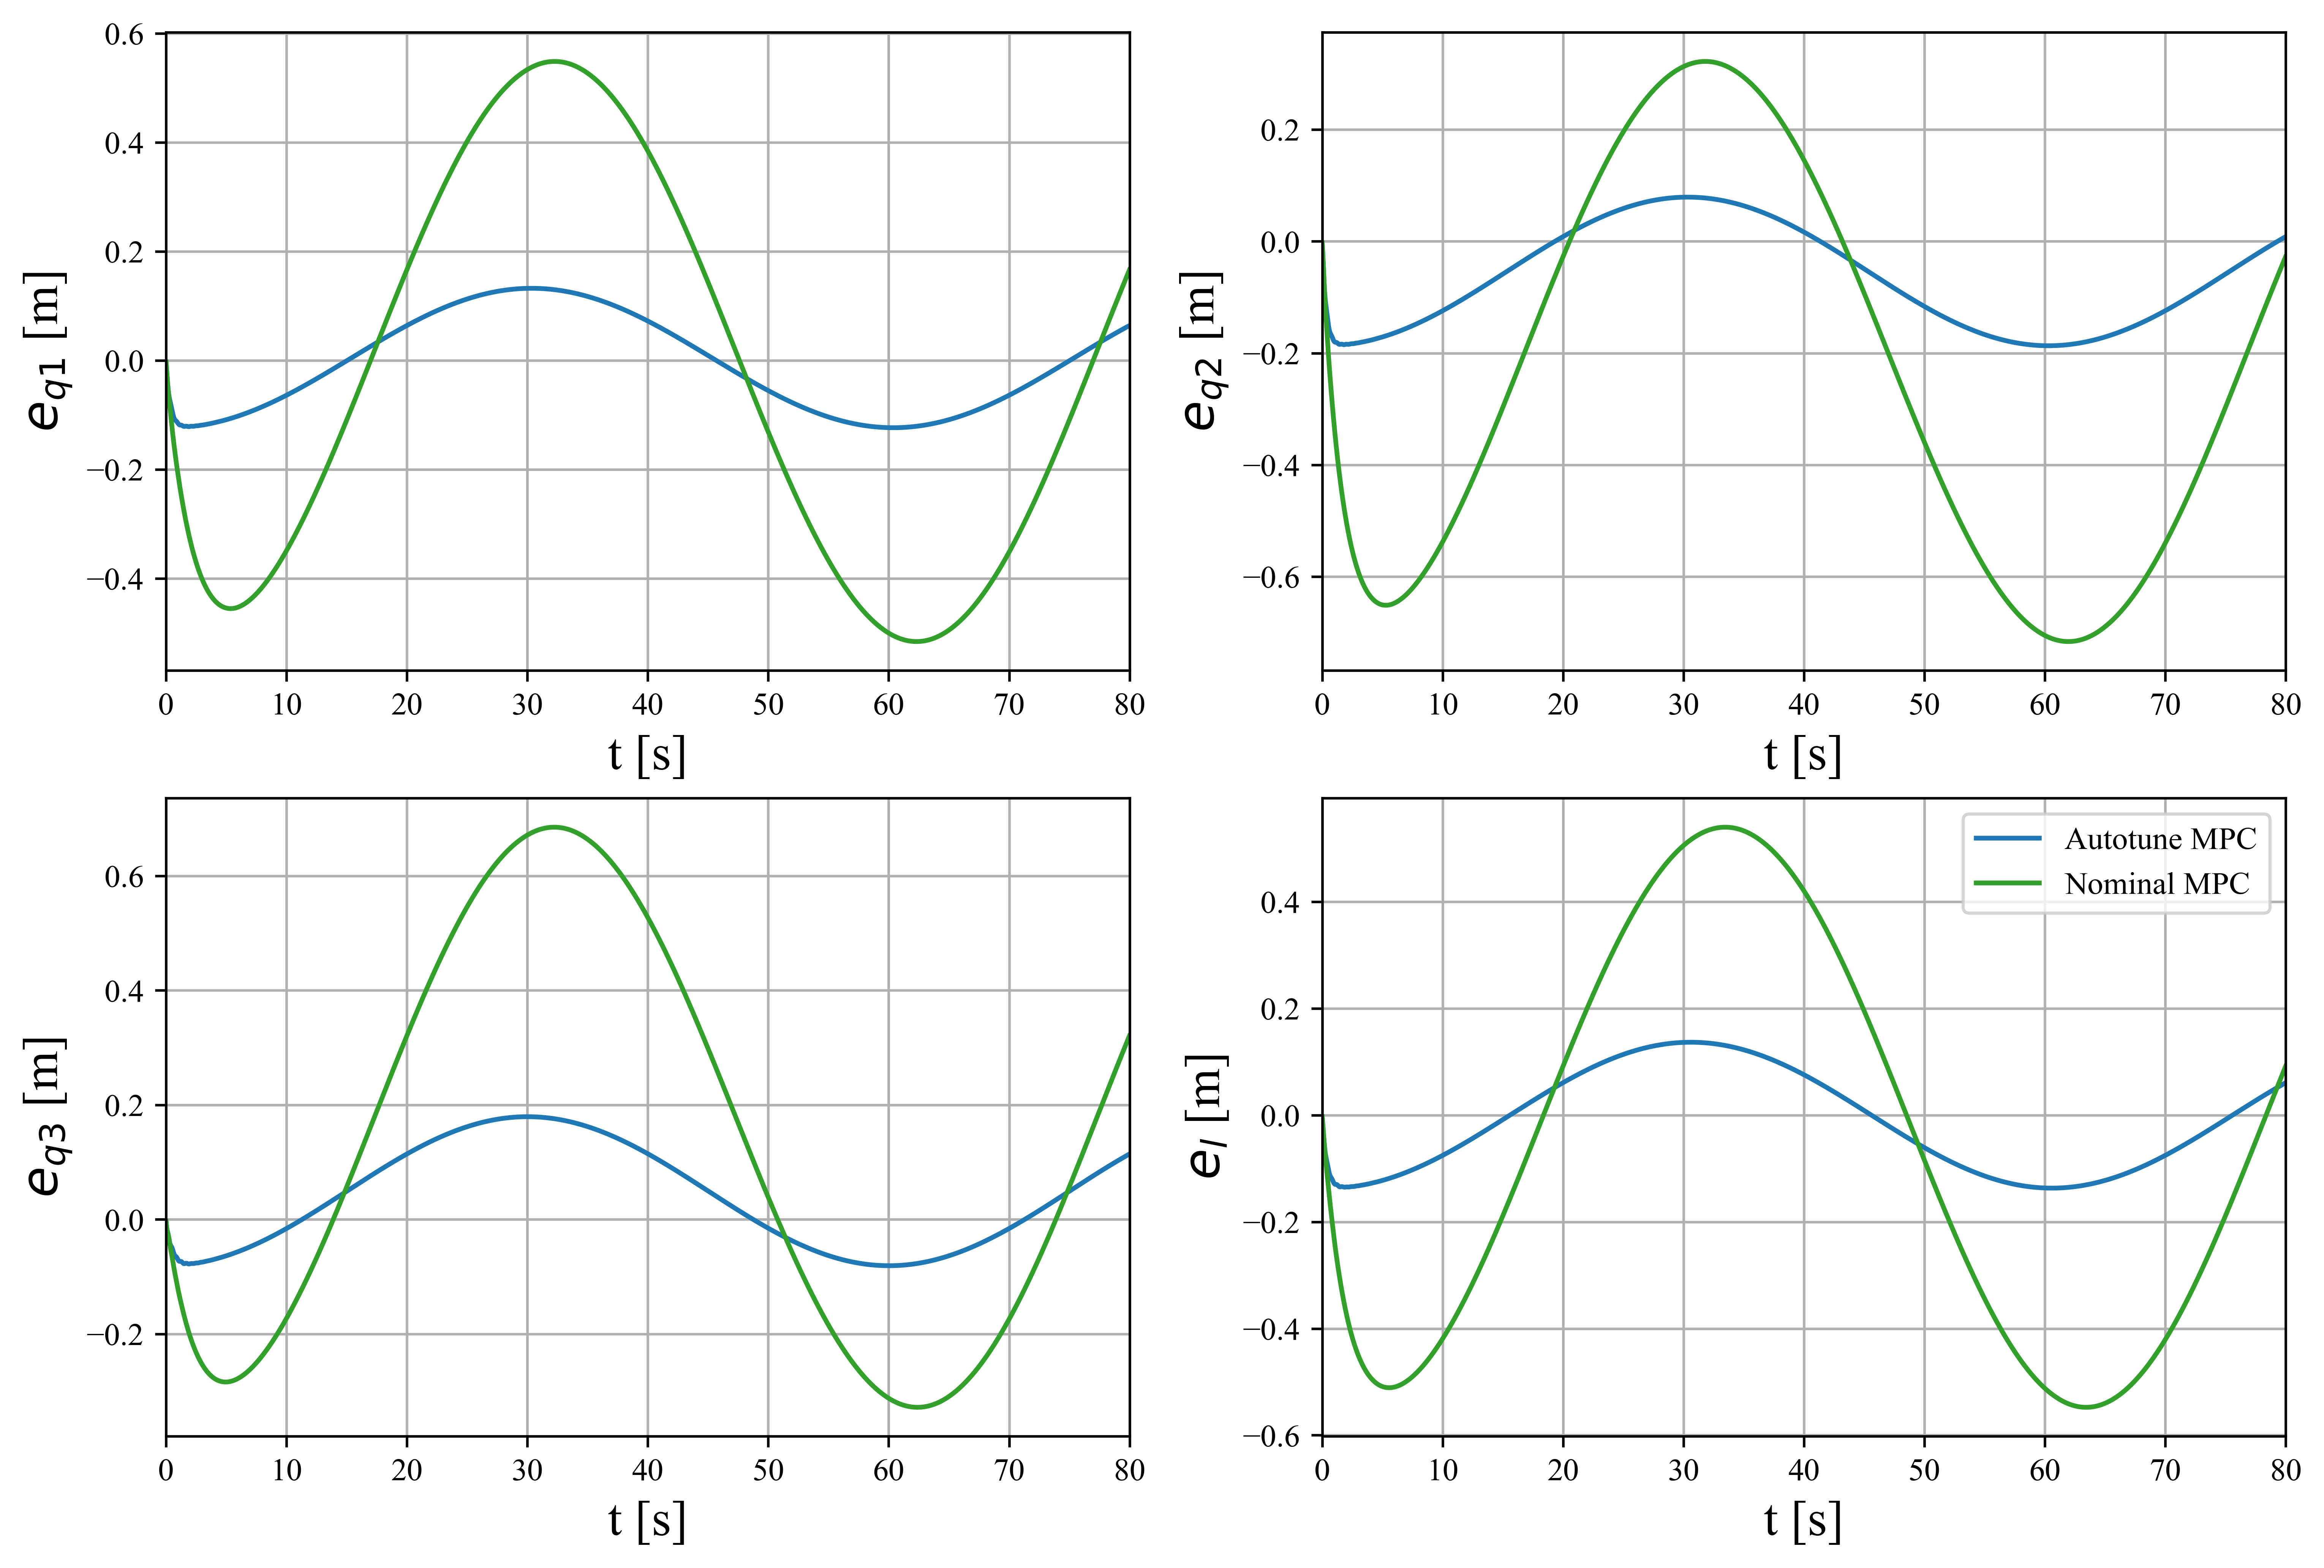
\includegraphics[width=38pc]{picture/kk2/ey.png} 
	\caption{多无人机和载荷Y轴上的跟踪误差} 
	\label{ey}
\end{figure}

\begin{figure}[H]
	\centering
	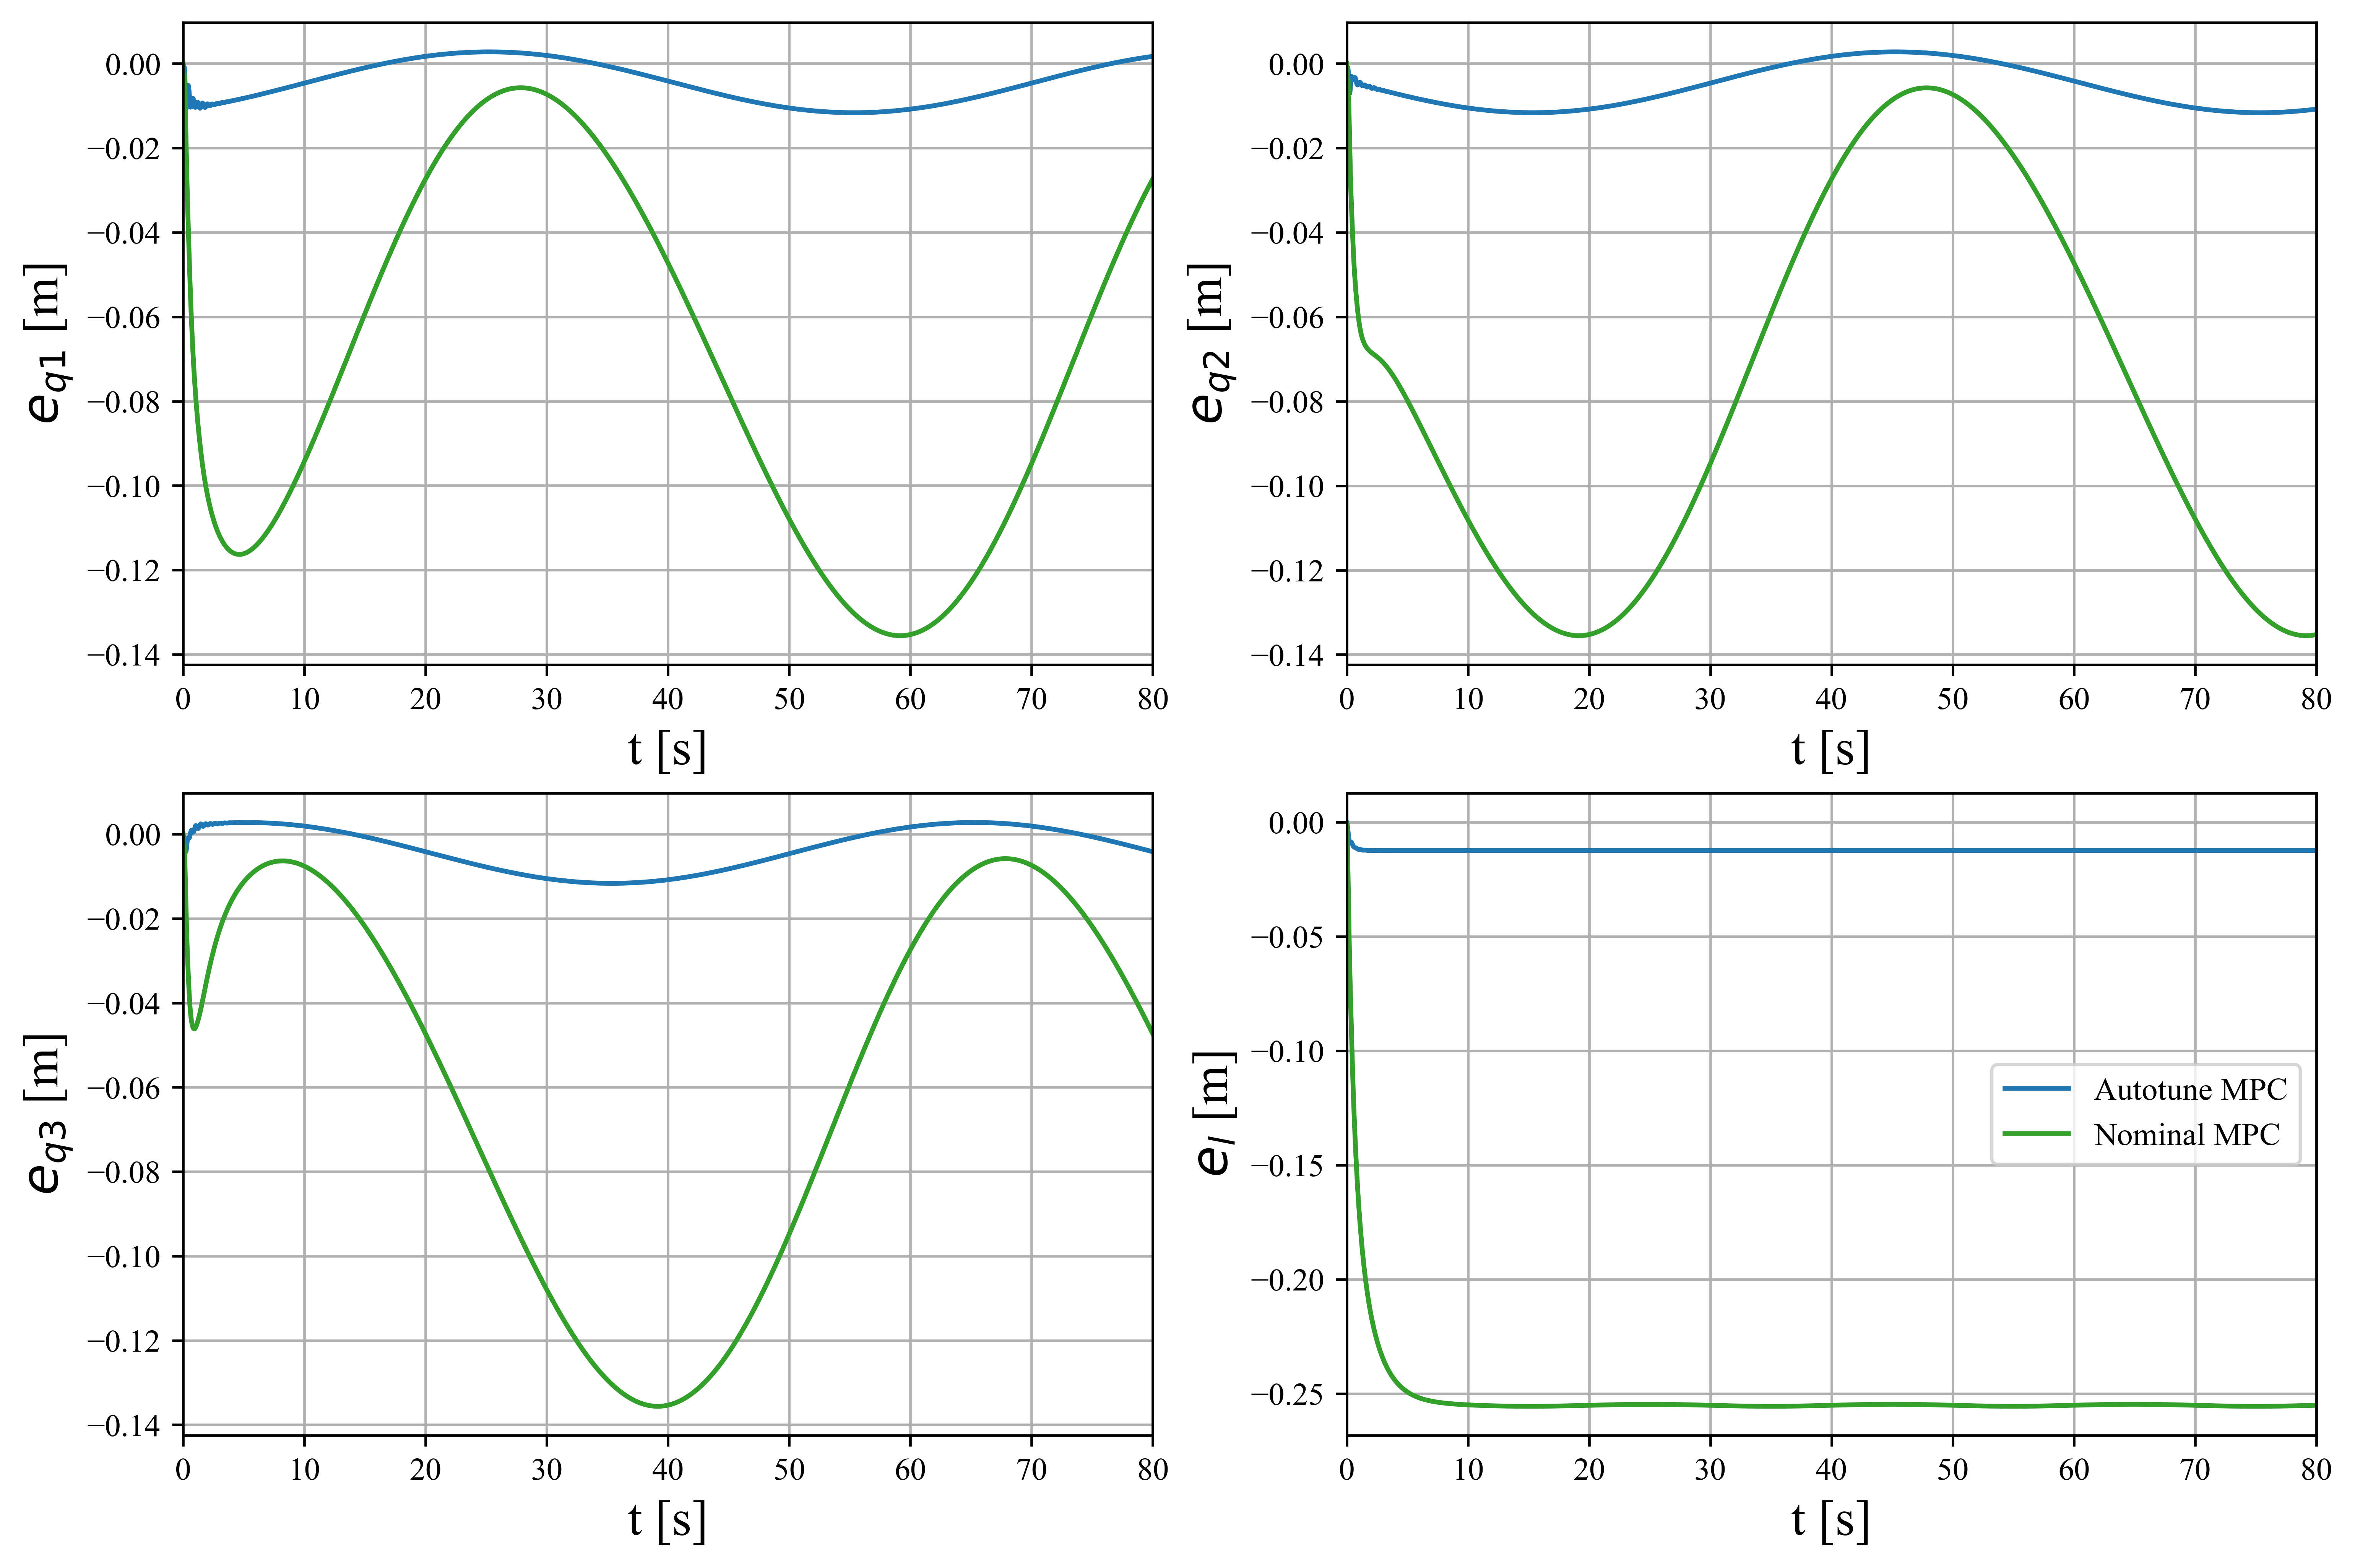
\includegraphics[width=38pc]{picture/kk2/ez.png} 
	\caption{多无人机和载荷Z轴上的跟踪误差} 
	\label{ez}
\end{figure}

\begin{figure}[H]
    \centering
    \begin{subfigure}[b]{0.49\textwidth}
        \centering
        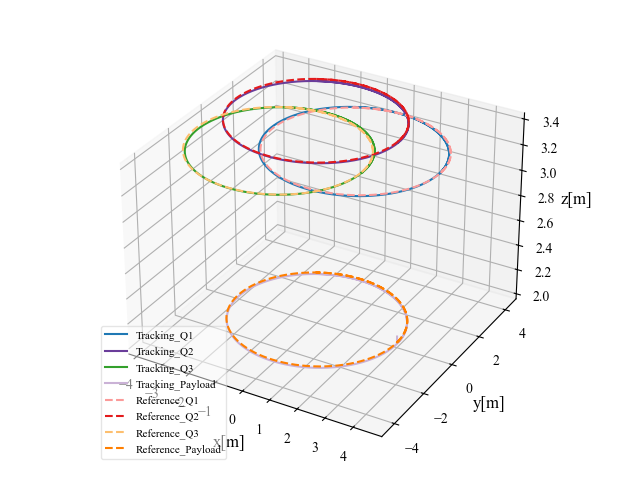
\includegraphics[width=\textwidth]{picture/kk2/3D.png} 
        \caption{Nominal MPC} 
        \label{3D1}
    \end{subfigure}
	\hspace{0.0\textwidth}
    \begin{subfigure}[b]{0.49\textwidth}
        \centering
        \includegraphics[width=\textwidth]{picture/kk2/plot3D.png} 
        \caption{Autotune MPC}  
        \label{3D2}
    \end{subfigure}
    \caption{三维空间下圆轨迹跟踪效果图}
    \label{combined3D}
\end{figure}

\section{试验系统介绍}   

试验系统包括硬件平台和软件平台两部分。硬件平台由动作捕捉设备、地面控制站和无人机构成,稳定的硬件平台能够保证所研究算法的可靠性;软件平台由控制模块和通信模块组成,是控制算法的载体。
通过硬件平台和软件平台的有机结合,试验系统能够在复杂环境中实现自主飞行、数据采集和算法验证等功能,满足多样化的应用需求。

\subsection{硬件配置}
\begin{figure}[hbt!]
	\centering
	\includegraphics[width=36pc]{picture/5_4.png} 
	\caption{室内试验系统信息流传递图} 
	\label{framework}
\end{figure}
由于无人机吊运控制算法在实地测试中需要精确获取自身位置,但在室外环境中,受地形复杂、信号干扰和气候条件等因素的限制,难以实现高精度的绝对位置测量。因此,试验选择在室内环境进行测试,采用动作捕捉设备测定无人机的位姿。地面控制站接收位姿信息并传递给地面站,地面站通过路由器远程连接各无人机,运行算法进行验证。整个系统的信息流的传递图如图 \ref{framework} 所示。


动作捕捉设备选用NOKOV(度量)光学三维动作捕捉系统,该系统采用20个高性能红外摄像头捕捉反光标识点,采集并生成精准、实时的动作信息,可广泛应用于无人机室内定位追踪、多智能体协同控制等领域。每个无人机上都会安装四个非共面的反光标识点,并通过四个反射球创建一个刚体,动作捕捉设备能够高精度地解算出刚体的位姿,并提供亚毫米级精度的高频实时位姿估计,具有抗干扰能力强、稳定性高的特点,为算法的验证和性能评估提供了可靠的参考基准。

地面控制站即 Mocap计算机,可实现多个无人机之间的通信、遥控器通道的设置、 动作捕捉设备位姿数据的读取和转换、无人机的控制和指令生成以及整体任务的规划等。机载计算设备与Mocap计算机通过局域网建立连接,Mocap计算机将解算得到的位姿信息通过路由器进行广播,无人机上的机载计算设备在接入路由器的局域网后使用VRPN协议可以获取得到广播的实时位姿信息。同时,地面站通过路由器的局域网ssh连接至无人机的机载计算设备,可以对无人机发布控制命令并监控其自身状态。

无人机平台的硬件选择主要考虑了算力、重量及接口等因素。试验平台选用了Orange Pi 5开发板作为机载计算设备,如图 \ref{fig.fmtpath} 所示,Orange Pi 5配备了Rockchip RK3588S处理器,这是一款高性能八核 ARM Cortex-A76 和 Cortex-A55 的混合架构处理器,提供强大的CPU计算性能,同时支持 GPU 和 NPU 加速。此外,Orange Pi 5的薄型设计和轻巧重量使其能够轻松地安装在无人机上,同时提供了丰富的接口,适配多种外设。在下位机选择方面,无人机平台采用了香港科技大学-大疆创新科技联合试验室基于PX4开源项目开发的NxtPX4v2飞控系统,如图 \ref{fig.proximity-tra} 所示,该飞控采用了STM32H743VIH6主处理器和双BMI088 IMU冗余传感器组,设计迷你小巧,安装孔间距为标准的20*20mm,可以在大多数小型穿越机机架上安装,具有高效、可靠的控制算法,能够处理复杂的动态控制任务,确保四旋翼在各种飞行状态下的稳定性和响应速度,并在最大程度上保障飞行任务的执行。

\begin{figure*}[htb!]
    \centering
    \begin{minipage}[t]{0.96\textwidth}
        \centering
        \begin{subfigure}[t]{0.47\textwidth}
            \centering
            \includegraphics[height = 1.85in]{picture/5_5.png}
            \caption{Orange Pi 5开发板\label{fig.fmtpath}}
        \end{subfigure}\hfill
        \begin{subfigure}[t]{0.47\textwidth}
            \centering
            \includegraphics[height = 1.95in]{picture/5_6.png}
            \caption{NxtPX4v2飞控\label{fig.proximity-tra}}
        \end{subfigure}
    \end{minipage}
    \caption{无人机硬件控制系统图}
\end{figure*} 
在无人机平台的机械部分设计中,机架的选择至关重要,其决定了可以安装的最大桨叶尺寸、电池大小等。本文选择了自制的3.5寸机架,采用双层碳板结构的机臂和中心板,并通过铝柱连接,既轻便又具备较高的强度。为了充分利用空间使无人机的结构更加紧凑,机载计算设备置于机架顶部,下位机飞控和电子调速器置于机架底部,并用底层板保护,这样布局可以更好地对无人机的控制能力进行验证。在动力系统方面,电机选用了四个T-Motor F2004无刷电机,电子调速器采用蓝鸟48K 30A四合一电调,桨叶选用了两对QProp DT90自锁3叶正反尼龙桨,为无人机提供平稳、精准的动力输出。电池方面,选择了格氏金砖系列6s1p 1050mAh 95C锂电池组,相比于5s电池,6s电池提供更强的动力,可直接对Orange Pi 5供电,满载测试续航时间为6分钟,能够满足试验需求。定制的无人机重1.0 kg,电机轴距为360 mm。最后, 对其他的安装件位置进行设计,包括电池固定件、接收机、数传和降压模块等。最终得到无人机的设计图和实物图如图 \ref{Fig.proximity} 所示。
\begin{figure*}[htb!]
	\centering
	\begin{minipage}[t]{0.96\textwidth}
		\centering
		\begin{subfigure}[t]{0.47\textwidth}
			\centering
			\includegraphics[height = 2.25in]{picture/5_7.jpg}
			\caption{SOLIDWORKS设计图\label{fig.path}}
		\end{subfigure}\hfill
		\begin{subfigure}[t]{0.47\textwidth}
			\centering
			\includegraphics[height = 2.25in]{picture/5_8.jpg}
			\caption{实物图\label{fig.proximity}}
		\end{subfigure}
	\end{minipage}
	\caption{无人机平台设计图和实物图\label{Fig.proximity}}
\end{figure*}



\subsection{软件配置}
试验平台的软件环境为无人机绳系吊运系统在通信层提供支持,并提供了算法的运行等基本环境,所采用的算法基于 Ubuntu 22.04 和 ROS 2 Humble 进行部署。ROS 2 相较于 ROS 1 在多个关键方面展现出显著优势,显著提升了机器人软件开发的效率和系统性能。ROS 2 采用实时中间件 DDS,增强了系统的实时性和确定性,满足了高实时性应用的需求,其分布式架构和基于 DDS 的通信机制提升了系统的扩展性和多机器人协同能力,同时引入了身份认证和数据加密等安全特性,确保了数据传输的安全性。模块化设计和 colcon 包管理系统提高了系统的可扩展性和可维护性,现代化工具链如 rviz 2 简化了开发、测试和部署流程。此外,ROS 2 拥有活跃的社区和丰富的开源资源,众多开发者基于ROS 2开发应用,并将成熟的代码开源到社区中,促进了ROS 2生态系统的快速扩展。本文中,ROS 2通过基于colcon的构建和包管理方案、部分底层设备驱动、多线程管理以及进程间通信方案得以应用。

\begin{figure}[hbt!]
	\centering
	\includegraphics[width=27pc]{picture/ros.png} 
	\caption{通信信息流示意图} 
	\label{ros}
\end{figure}
图 \ref{framewor} 展示了算法在试验过程中所使用的主要软件包及其间传递的消息内容。在飞行试验中,动作捕捉设备以100Hz的频率提供外部绝对定位信息,并通过无线连接传递给飞控系统,与飞控系统中的传感器数据进行融合并作为源数据使用。
无人机控制程序采用C++语言编写,机载计算设备通过USB转串口线与飞控系统连接,通信波特率设置为921600。主程序首先定义了发送和接收的数据类型,涵盖了输出推力、姿态角、位置信息以及以四元数表示的姿态数据。控制算法由定时器以20毫秒的周期触发运行,计算结果通过 uXRCE-DDS 中间件传输至飞控系统以执行相应操作。
uXRCE-DDS(Micro XRCE-DDS) 是由 eProsima 开发的一种轻量级通信中间件,旨在为资源受限的嵌入式设备提供与标准 DDS(Data Distribution Service)生态系统的无缝集成。它基于 XRCE(规范,专为微控制器和其他受限硬件环境设计,确保在低功耗和有限计算资源的设备上实现高效的实时数据分发和通信,这为 PX4 和 ROS 2 之间提供了快速可靠的集成,并使 ROS 2 更容易获取无人机自身信息以及发送指令,从而更精确地实现了无人机的控制和数据传输。这种节点式的通信方法如图 \ref{ros} 所示,这些节点被封装在易于共享和发布的程序包和功能包中。ROS 2的节点式通信基于TCP和UDP协议,因此用户无需关注底层通信的管理。每个节点发布一个Topic,其他节点可以选择订阅这些消息。这样,无人机的各个模块可以在单个无人机内部进行通信,也可以在不同无人机之间进行信息交换。每个无人机通过读取传感器数据,并通过滤波和融合算法计算出位姿信息,再通过ROS 2节点进行发布。其他无人机可以选择性地订阅相关信息,从而实现分布式控制。该方式简洁、稳定且可靠。
QGC地面站提供数据监控和指令功能,用于监控数据以及申请自主飞行模式(Offboard模式)。需要特别指出的是,尽管上位机也具备申请自主飞行模式的功能,但为了确保飞行试验的安全性,禁止通过上位机进行此类申请,自主飞行模式的切换仅通过遥控器和地面站执行。
\begin{figure}[hbt!]
	\centering
	\hspace{1.0cm}
	\includegraphics[width=28pc]{picture/5_10.png} 
	\caption{室内飞行试验设置示意图} 
	\label{framewor}
\end{figure}

\section{无人机绳系吊运系统控制试验验证}
如图 \ref{framewor} 所示,在真实飞行试验的设置中,无人机配备了PX4硬件飞控系统,用于实现精确的姿态估计和低级别控制。无人机的位置和线性速度通过动作捕捉设备进行实时估计,其具有高精度的空间定位能力,可为无人机提供准确的位置和速度数据,从而为MPC提供关键输入。此外,加速度和角速度则通过PX4内置的加速度计和陀螺仪传感器进行测量。这些传感器能够实时采集无人机的加速度和旋转速率数据,为系统提供必要的状态信息,确保飞行控制的精确性和实时性。在实机算法中,MPC优化问题的求解采用CasADi \cite{Andersson2019} 和 acados \cite{Verschueren2022} 进行部署。
\subsection{单无人机吊运试验验证}
\begin{figure}[hbt!]
	\centering
	\includegraphics[width=28pc]{picture/danjireal.png} 
	\caption{无人机试验场景} 
	\label{dan}
\end{figure}
对于单无人机吊运试验,无人机试验场景如图 \ref{dan} 所示。在训练数据以50 Hz的频率采集,数据来源于沿圆轨迹飞行的无人机数据来源于沿圆轨迹飞行的无人机,该系统采用MPC进行控制。训练数据集仅包含60秒的飞行数据(共3000个数据点),这些数据用于训练模型,外力和力矩通过\autoref{nmpc}计算后作为标签用于学习。在数据采集过程中,系绳长度和载重分别为0.8 m和160 g,这些参数在NP-MPC中是未知的,因此在训练过程中,系统必须基于实时估计的状态信息来动态调整控制策略。考虑到这些参数的不确定性,NP-MPC通过建模外力和力矩对飞行控制进行实时预测,从而确保系统在没有先验信息的情况下仍能稳定运行。

\begin{figure}[hbt!]
	\centering
	\includegraphics[width=34pc]{picture/kk/force.png} 
	\caption{在载荷上添加额外重量时Neural Predictor对Z轴方向外力的估算结果} 
	\label{force}
\end{figure}
首先,展示了Neural Predictor在准确预测外力方面的能力。在试验中,当无人机的载荷为160 g、悬停高度为1.6 m时,向载荷上附加了一个额外的100 g砝码。外力的预测结果如图 \ref{force} 所示。从试验结果可以看出,Neural Predictor对外力变化的动态响应几乎是即时的,能够迅速反映载荷变化带来的外力变化。当载荷重量增加100 g时,Neural Predictor的输出值增加了0.96 N,且标准差为0.04 N,这表明其预测具有较高的精度和稳定性。值得注意的是,由于四旋翼系统在飞行过程中存在一定的残差力和力矩,即系统的惯性和其他飞行动力学因素可能导致短暂的响应偏差,Neural Predictor的输出变化并不完全等于附加载荷的重力变化。
总体而言,这些结果表明,Neural Predictor能够在飞行过程中实时且准确地估计外力,并能够有效适应不同的未知载荷,在各种飞行环境中进行外力预测,尤其在动态变化的环境下表现出较强的适应性和鲁棒性。

其次,开展了实际飞行轨迹跟踪试验,以验证NP-MPC在轨迹跟踪方面的优越性,并将其与MPC、GP-MPC \cite{torrente2021data} 和 KNODE-MPC \cite{Chee2022} 这三种算法进行对比分析,其中GP-MPC和KNODE-MPC均为基于数据驱动的模型预测控制方法。为了确保对比的公平性,三种基于数据驱动算法的训练数据集均来自于上述数据采集试验中的60秒圆形飞行轨迹。
在算法实现方面,KNODE网络模型的架构与升维函数$\Psi$相同,保证了其在处理复杂动态时的适应性。GP模型则采用径向基函数(RBF)作为核函数,并使用100个数据点进行训练,这些数据点按规则间隔采样,确保模型能够捕捉到轨迹中的关键特征。对于NP、GP和KNODE模型的输入,它们均为四旋翼的线性速度和角速度,这些输入在实际飞行试验中被实时采集并用于轨迹跟踪控制。
参考信号的生成采用多项式轨迹生成器,确保参考轨迹具有平滑的变化和较小的误差。试验中的参考高度设定为1.6 m,载荷重量为160 g。通过对比NP-MPC与其他算法的表现,能够评估其在实际飞行环境中的鲁棒性、实时性以及对不同载荷和轨迹的适应能力。

\renewcommand\arraystretch{1.15}
\begin{table}[htb!]
    \centering
    \caption{在两条实际飞行轨迹上的跟踪误差(RMSE)的比较结果}
    \label{table_xyz}
    \renewcommand\arraystretch{1.5} % 调整行间距,使表格更大
    \begin{tabular}{m{2.2cm}<{\centering} m{2.5cm}<{\centering} m{2.2cm}<{\centering} m{2.2cm}<{\centering}}
        \Xhline{1.pt}
        \textbf{飞行轨迹} & \textbf{算法} & \textbf{$\bm E_{xy}$ [m]} & \textbf{$\bm E_z$ [m]} \\
        \Xhline{1.pt}
        & Nominal MPC & 0.1797 & 0.2329 \\
        \multirow{2}{2.2cm}{\centering {圆}} & GP-MPC & 0.1414 & 0.1692 \\
        & KNODE-MPC & {0.0919} & {0.1307} \\
        & NP-MPC & \textbf{0.0837} & \textbf{0.0758} \\
        \hline
        & Nominal MPC & 0.2029 & 0.2539 \\
        \multirow{2}{2.2cm}{\centering {双纽线}} & GP-MPC & 0.1878 & 0.1966 \\
        & KNODE-MPC & {0.1503} & {0.1406} \\
        & NP-MPC & \textbf{0.0849} & \textbf{0.0591} \\
        \hline
        \Xhline{1.pt}
    \end{tabular}    
\end{table}
\begin{figure}[hbt!]
	\centering
	\includegraphics[width=38pc]{picture/kk/color.png} 
	\caption{不同MPC算法在飞行速度 1.5 m/s 下的飞机轨迹跟踪性能对比} 
	\label{color}
\end{figure}
四种框架在跟踪持续50秒的两条轨迹时的性能结果如表 \ref{table_xyz} 和图 \ref{color} 所示。值得注意的是,由于载荷的重力对无人机造成的影响,MPC在X-Y平面和Z轴的轨迹跟踪误差表现显著。而三种基于数据驱动的算法(GP-MPC、KNODE-MPC和NP-MPC)通过捕捉数据中的外力和力矩,成功减少了跟踪误差,优于MPC。在圆形轨迹跟踪试验中,GP-MPC、KNODE-MPC和NP-MPC均表现优于NMPC,因为它们能够从数据中学习到动力学模型的残差项,并对模型中的未知动力学进行了补偿。

具体而言,提出的NP-MPC在X-Y平面上减少了53.45\%的跟踪误差,在Z轴上减少了67.45\%,相较于MPC取得了显著的改进。在双纽线轨迹跟踪试验中,GP-MPC、KNODE-MPC和NP-MPC的跟踪表现同样优于MPC。然而,当参考轨迹的曲率半径较小时,GP-MPC和KNODE-MPC的跟踪误差较大,而NP-MPC能够在曲率半径较小的情况下,仍然精确地跟踪参考轨迹。需要注意的是,双纽线轨迹在形状上与训练数据集中的圆形轨迹存在一定差异,在双纽线轨迹跟踪试验中,NP-MPC在X-Y平面减少了58.16\%的跟踪误差,在Z轴减少了76.72\%,相较于MPC表现更为出色。这些结果表明,NP-MPC在不同类型轨迹下,尤其在复杂几何形状和较小曲率的轨迹跟踪任务中,能够有效地降低误差并提升跟踪精度,同时具有一定的泛化能力。

\begin{figure}[hbt!]
	\centering
	\includegraphics[width=34pc]{picture/kk/prediction_res.png} 
	\caption{在载荷上添加额外重量时Z轴方向外力的估算结果} 
	\label{prediction_res}
\end{figure}
最后,为了充分验证所提NP-MPC的泛化性能,本试验采用了训练数据集之外的速度数据和有效载荷质量进行测试,旨在评估其在不同环境和条件下的表现。具体而言,本试验设计了四种测试场景,其中第一个场景用于收集数据集,并在该数据集上训练神经网络模型。然后,基于此训练好的模型,进一步设计了三种不同的测试情况以检验NP-MPC的泛化能力:第一种情况是改变飞行速度的大小,第二种情况是改变飞行轨迹的半径,最后一种情况则是增加有效载荷的额外重量。这三种不同的测试场景可以模拟实际应用中可能出现的变化条件,从而验证所提方法的适应性和鲁棒性。
在图 \ref{prediction_res} 中,分别展示了在不同速度、轨迹半径和有效载荷情况下的测试结果。从中可以明显看出,NP-MPC相比于传统的MPC在所有测试场景中均展现出了更优的跟踪性能。在所有测试场景下,跟踪精度的提升最大可达到65.1\%。尤其在增加有效载荷额外重量的情况下,NP-MPC凭借其快速响应和准确预测的能力,能够迅速适应载荷变化,从而将跟踪精度提升至76.39\%。这一结果表明,NP-MPC在面对实际应用中的动态变化时,能够有效提升轨迹跟踪的精度和稳定性。上述试验的结果表明,NP-MPC具有很强的泛化能力,能够有效地适应训练数据集领域之外的未见数据。

\subsection{多无人机吊运试验验证}
对于多无人机吊运试验,在载荷上也安装三个非共面的反光标识点用动作捕捉设备的位姿进行精准实时估计。为了增强飞行试验中无人机的可靠性,避免系统失效,进一步缩小自适应 MPC 权重的上限,上下限分别设定为0.01和1。多无人机吊运系统的系绳长度和载重分别为 1.2 m 和 1.5 kg。

本次试验旨在验证 Autotune-MPC 在多无人机绳系吊运系统中在飞行试验中的应用效果,尤其是其在复杂轨迹跟踪任务中的优越性与实用性。试验通过多项式轨迹生成器生成了三架无人机和载荷的实际飞行轨迹,采用传统的MPC和 Autotune-MPC 两种不同的控制策略进行比较,评估其在动态跟踪和自适应调整中的性能。

\begin{figure}[H]
	\centering
	% 第一行的两张图
	\begin{subfigure}[b]{0.48\textwidth}
		\centering
		\includegraphics[width=\textwidth]{picture/kk/4.png}
		\caption{无人机1}
		\label{quadrotor00}
	\end{subfigure}
	\hfill
	\begin{subfigure}[b]{0.48\textwidth}
		\centering
		\includegraphics[width=\textwidth]{picture/kk/5.png}
		\caption{无人机2}
		\label{quadrotor01}
	\end{subfigure}
	
	\vspace{0.5cm} % 调整两行之间的垂直间距
	
	% 第二行的两张图
	\begin{subfigure}[b]{0.48\textwidth}
		\centering
		\includegraphics[width=\textwidth]{picture/kk/6.png}
		\caption{无人机3}
		\label{quadrotor02}
	\end{subfigure}
	\hfill
	\begin{subfigure}[b]{0.48\textwidth}
		\centering
		\includegraphics[width=\textwidth]{picture/kk/8.png}
		\caption{载荷}
		\label{load0}
	\end{subfigure}
	
	\caption{多无人机和载荷位置跟踪的试验结果}
	\label{t}
\end{figure}

在试验开始阶段,首先采用手动调参的传统 MPC 控制器对多无人机绳系吊运系统进行控制。MPC 控制器在该阶段通过精确的建模和手动设置的参数,实现了系统的初步稳定,并将三架无人机带到轨迹的起始点,开始对设定的轨迹进行跟踪。无人机和载荷的初始轨迹跟踪表现良好,但由于系统的强耦合性和复杂性,传统 MPC 控制器的固定参数在复杂环境中无法充分适应系统的动态变化,因此存在一定的轨迹误差和控制不稳定的风险。


在轨迹跟踪试验进行到第 9 秒时,系统开始启用 Autotune 功能。Autotune-MPC 通过实时的自适应调参机制,对 MPC 控制参数进行动态调整,以适应环境变化和系统的非线性特性。在这一过程中,Autotune 功能根据当前飞行状态和环境信息,自动调整控制器的增益、约束和权重,以提高控制系统的响应速度、精度和稳定性。如\autoref{t} 所示,在实际轨迹跟踪过程中,位置跟踪效果得到了明显改善。在启用传统 MPC 控制时,系统的轨迹跟踪存在一定的误差,尤其是在多无人机协同飞行和载荷运动的过程中,由于强耦合性和不稳定因素,误差较大。通过启用 Autotune-MPC 后,轨迹跟踪误差显著减少,系统轨迹逐步趋近于设定轨迹,飞行的平滑度和稳定性得到了显著提升。具体而言,传统 MPC 控制下的系统在轨迹跟踪的初期和中期,由于无法实时适应载荷变化和环境波动,误差较大;然而在 Autotune-MPC 启用后,随着控制参数的自动调整,系统的跟踪误差逐渐收敛,并且控制系统能够在不同的飞行阶段保持较高的精度,轨迹偏差逐步趋于理想值。

\begin{figure}[H]
	\centering
	% 第一行的两张图
	\begin{subfigure}[b]{0.48\textwidth}
		\centering
		\includegraphics[width=\textwidth]{picture/kk/1.png}
		\caption{无人机1}
		\label{quadrotoru0}
	\end{subfigure}
	\hfill
	\begin{subfigure}[b]{0.48\textwidth}
		\centering
		\includegraphics[width=\textwidth]{picture/kk/2.png}
		\caption{无人机2}
		\label{quadrotoru1}
	\end{subfigure}
	
	\vspace{0.5cm} % 调整两行之间的垂直间距
	
	% 第二行的单张图居中
	\begin{subfigure}[b]{0.48\textwidth}  % 调整宽度可以根据需要修改
		\centering
		\includegraphics[width=\textwidth]{picture/kk/3.png}
		\caption{无人机3}
		\label{quadrotoru2}
	\end{subfigure}
	\caption{无人机的虚拟控制输入}
	\label{u}
\end{figure}


在\autoref{u} 中,给出了三架无人机的虚拟控制输入。启用 Autotune 功能后,无人机的控制输入表现出了明显的变化趋势。起初,由于传统 MPC 的控制参数较为固定,无人机的控制输入较为剧烈,可能导致不必要的震荡。随着 Autotune-MPC 的启用,控制输入逐渐趋于平稳,系统能够根据实时飞行状态和环境变化进行参数调整,使得控制输入更加精准和高效。与传统控制方法相比,Autotune-MPC 的动态调整显著降低了控制输入的波动,提升了控制稳定性与飞行安全性。

\begin{figure}[H]
	\centering
	\includegraphics[width=28pc]{picture/kk/7.png} 
	\caption{载荷的姿态变化结果} 
	\label{x}
\end{figure}
在\autoref{x} 中,给出了载荷的姿态曲线,进一步验证了 Autotune-MPC 在姿态控制方面的优越性。在使用传统 MPC 时,载荷的姿态偏差较大,尤其是在飞行初期,载荷的姿态偏差幅度最大达到了 30 度。这种较大的偏差可能会导致载荷的不稳定运动,并影响到整个系统的控制效果。而在启用 Autotune-MPC 后,系统自动调整控制参数,使得载荷的姿态偏差逐渐减小。经过自适应调整后,载荷的姿态偏差明显减少,并趋近于 0 度,飞行过程中的载荷姿态得到了有效的平稳控制。这一结果表明,Autotune-MPC 能够实时感知载荷运动的变化,并通过动态优化控制参数来减少姿态误差,提升系统的整体稳定性和飞行控制效果。

试验结果表明,Autotune-MPC 在复杂的多无人机协同飞行和载荷控制任务中,能够有效提升系统的响应速度、精度和稳定性,显著减少轨迹跟踪误差和姿态偏差。此外,Autotune-MPC 的自适应调参功能,使得系统能够保持较高的跟踪精度,降低了对手动调参的依赖,能够有效适应不同载荷和环境变化,在动态飞行任务中展现出更高的灵活性和鲁棒性。


\section{本章总结}
本章搭建了无人机绳系吊运系统的物理引擎仿真平台和飞行试验平台,物理引擎仿真平台比较了几种主流的开源仿真平台并选取最优的平台进行仿真试验,飞行试验平台从硬件配置和软件配置两个方面来进行介绍并进行飞行试验。试验结果表明,无论是定点悬停还是轨迹跟踪,第3章提出的NP-MPC和第4章提出的Autotune-MPC均具有更好的控制效果。

\cleardoublepage

\chapter{总结与展望}
\chaptermark{总结与展望}


\section{本文工作总结}
本文围绕数据驱动方法在无人机绳系吊运系统中的应用展开研究,旨在解决单无人机吊装载荷的高精度跟踪与多无人机协同稳定控制问题。通过从系统建模、控制算法设计到仿真验证与实验研究的系统性探索,逐步构建了完整的研究框架,主要工作总结如下:

(1)动力学模型的建立与简化:
本文首先推导了单无人机绳系吊运系统的动力学模型,采用牛顿-欧拉法建立四旋翼无人机动力学方程,并通过拉格朗日方法对吊挂载荷进行建模。在多无人机系统中,通过拉格朗日方程求解系统动力学模型,并针对载荷状态未知的复杂情况,使得动力学描述更加贴近实际应用场景。

(2)基于数据驱动建模的单无人机吊运控制:
针对无人机绳系吊运系统中的不确定性和非线性干扰问题,本文提出了一种基于数据驱动的控制框架。引入Koopman算子理论,通过深度神经网络学习系统动力学,将无人机和载荷运动升维映射到显式线性空间中。在此基础上,结合模型预测控制方法,对无人机吊运系统的动力学进行精确建模与控制,显著提高了轨迹跟踪的精度与稳定性。

(3)基于数据驱动调参的多无人机协同控制:
在多无人机协同吊运场景下,本文提出了一种自适应超参数调参方法。结合分布式模型预测控制和灵敏度传播方法,使用分布式策略梯度学习生成自适应超参数并集成到模型预测控制中。该方法利用多层感知网络实现超参数自适应归一化,从而提高系统的协同稳定性与容错能力。

(4)仿真与试验验证:
为验证所提算法的有效性,本文搭建了无人机绳系吊运系统的物理引擎仿真平台,选用Drake、Gazebo和MuJoCo等开源物理引擎对无人机吊运系统进行建模与仿真。结果表明,所提数据驱动控制方法能够有效跟踪期望轨迹,并在复杂环境中保持系统稳定性。此外,本文进一步搭建了无人机吊运系统的飞行试验平台,通过实地试验验证了算法在实际应用中的可行性与鲁棒性。

\section{未来工作展望}
在协同空中操控领域,无人机绳系吊运系统展现了极大的应用潜力。本文在基于数据驱动无人机绳系吊运系统控制算法方面取得了一定成果然而,现阶段的研究多在理想化环境下进行,通过假设、简化和近似,逐步迈向实际应用。基于上述内容,未来研究可重点关注以下方向:

(1)强化学习与自适应控制的结合:
未来研究可以将强化学习方法与数据驱动控制相结合,进一步提高无人机绳系吊运系统在动态复杂环境中的自主学习与适应能力。通过在线学习和实时更新控制策略,使系统能够在不确定环境中保持高效稳定的控制性能。

(2)下洗气流对载荷引起的阻力建模与补偿:
载荷在吊运过程中会受到下洗气流影响,特别是表面积大的载荷更容易产生较大阻力,进而引发系统稳定性下降。未来研究可针对不同载荷表面积和系绳长度,建立更加精细的阻力模型,并设计实时估计与补偿算法,以有效削弱下洗气流对载荷的扰动影响。

(3)多无人机系统中的通信与协同优化:
在多无人机协同吊运中,通信延迟与丢包问题可能对系统稳定性产生影响。未来可探索基于边缘计算或5G通信技术的分布式控制框架,进一步提高多无人机系统的响应速度与协同效率。

(4)复杂载荷与非结构化环境的适应性研究:
目前的研究主要针对规则载荷和理想环境下的吊运任务,未来可以拓展至不规则载荷及非结构化环境。通过结合计算机视觉和环境感知技术,实现对复杂载荷形态与外界环境的实时感知与反馈,从而提升无人机吊运系统在复杂场景中的应用能力。

(5)室外与视觉感知试验:本文试验多在室内无风环境下进行,利用运动捕捉系统简化感知与估计问题。然而,实际应用中无人机往往面临复杂的外部环境和不确定因素。未来研究应侧重于室外环境下的吊运试验,结合机载视觉传感器与高性能计算硬件,运行计算密集型感知算法,实现载荷姿态估计与目标定位。这将有效提升无人机在动态环境中的自主性和感知能力,减少对外部捕捉系统的依赖,进而推动无人机在仓储物流、灾害救援等场景中的实际应用。

综上所述,本文为无人机绳系吊运系统的稳定控制与协同作业提供了有效的解决方案,并为未来无人机运输系统的发展奠定了理论与实践基础。随着数据驱动技术与人工智能的不断发展,相信无人机绳系吊运系统将在更多复杂场景中展现出广阔的应用前景。





%%=============================================================================%
%% 参考文献以及附录
%%-----------------------------------------------------------------------------%
\bibliographystyle{nputhesis}                               % GB/T 7714-2015 格式
% \bibliographystyle{nputhesis-noslash}                       % 参考文献改进格式
\bibliography{reference}                                    % 参考文献
%%=============================================================================%
%% 文档附页部分(致谢、参加科研情况、知识产权与原创性声明)
%%-----------------------------------------------------------------------------%
\backmatter                                                 % 文档附页部分
%%-----------------------------------------------------------------------------%
%\bibliography{ref}

\begin{acknowledgements}                                    % 致谢开始
衷心感谢各位老师在百忙之中拨冗审阅本论文!
% 时光如白驹过隙,转眼间我的研究生生活即将画上句号。在西北工业大学航天学院的三年求学岁月里,我不仅收获了专业知识,锻炼了科研能力,更收获了无数宝贵的友情和深厚的师生情谊。在此,我怀着感恩的心情,衷心感谢所有在我的成长过程中给予帮助、支持和鼓励的每一位老师、同学和家人。

% 首先,我要衷心感谢我的导师张帆教授。张老师严谨的治学态度和孜孜不倦的工作精神一直是我学习的榜样。作为我的导师,张老师不仅在学术上给予我无微不至的指导,还为我提供了优越的科研条件,并始终关心和支持我的成长。在张老师的教诲和引导下,我不断完善自己的专业技能,逐步迈向科研的高峰。在此,向张老师表达我最深的感激之情。

% 其次,我要感谢张帆老师,张老师的支持与鼓励在我的研究生生涯中占据了重要的位置。她不仅是我的学术导师,更像是我亲切的大姐姐。无论是在课题的设计、实施过程中,还是在面对困惑和挫折时,张帆老师始终给予我极大的关怀和帮助。她总是耐心地为我解答问题,鼓励我在科研上不断突破自我,从不因困难而气馁。我深深感激张帆老师对我个人成长的悉心帮助与关爱。


% 最深沉的感激,属于我的父母。感谢他们一直以来对我的无私支持和鼓励。无论是生活中的点滴关怀,还是学业上的悉心照顾,父母为我提供了坚强的后盾。正是因为他们的辛勤付出和无怨无悔的奉献,才让我能够在求学的道路上无所畏惧、勇往直前。父母的恩情,我将铭刻一生,终身难忘。

% 在学术和生活上,我还要感谢王通师兄、刘习尧师兄、刘亚师姐。感谢你们在我遇到学术难题时耐心的解答和指导。你们不仅帮助我解决了试验中的技术问题,也让我在学术研究中不断完善自我。还要特别感谢我的同门杨立、文思捷和师弟金澳,感谢你们在我的试验研究过程中提供的宝贵意见和支持,帮助我克服了诸多技术和设计难题。

% 此外,我的室友、老大哥粟刚,是我研究生期间的另一位重要人物。感谢你在我忙碌的学术生活中,给予我生活上的关心与支持。你的乐观与积极,深深感染了我,带我领略了西安的风土人情,品尝了无数美食,让我在繁重的课业中,依然保持了热情与动力。

% 我还要感谢课题组的各位老师:马志强老师、常海涛老师、刘星老师、沈刚辉老师、张夷斋老师、刘正雄老师,感谢你们在科研工作中的指导和帮助。你们的经验和建议让我在科学研究的道路上少走了许多弯路。还要感谢韩冬、陈海飞、黄冰潇、李陇南、李沅澔、赵亚坤、王志祥、宋梦实、张校祯、余航、高家乐、裴崇旭、翟晨萌、杨通等师兄师姐,感谢你们在学术上和生活中给予的帮助与关怀,让我的研究生生活更加丰富多彩。

% 再次感谢所有在我求学旅程中给予过帮助的人。你们的支持与鼓励,是我不断前行的不竭动力。未来的路上,我将继续努力,不忘初心,勇敢追求更高的目标。
\end{acknowledgements}                                      % 致谢结束
%%-----------------------------------------------------------------------------%
\begin{accomplishments}                                     % 参加科研情况开始
	论文发表情况:
	\begin{enumerate}
		\item \blackbox{Ao Jin}, \blackbox{Chenhao Li}, \blackbox{Ya Liu}, \blackbox{Panfeng Huang} and \blackbox{Fan Zhang}. Neural Predictor for Flight Control with Payload [J].  IEEE Robotics
		and Automation Letters, 2024(中科院SCI 计算机科学类2 区, IF=4.6,一审中,第一作者)
	\end{enumerate}

    专利申请情况:
    \begin{enumerate}
    	\item \blackbox{张帆}, \blackbox{李晨豪}等. 一种柔性约束多智能体系统的协同运输鲁棒控制方法(发明专利,申请号/专利号:2024112841675,学生一作)
    \end{enumerate}

	项目参与情况:
    \begin{enumerate}
    	\item 基于多无人机协同作业的山区电力应急抢修载重运输关键技术研究,国网四川省电力公司科技项目
    	\item 空间绳系卫星地面气浮台实验系统,国家自然科学基金委重大研究计划重点支持类项目
    \end{enumerate}
\end{accomplishments}                                       % 参加科研情况结束
%%-----------------------------------------------------------------------------%
\makestatement                                              % 知识产权与原创性声明
%%=============================================================================%
%% 文档结束
%%-----------------------------------------------------------------------------%
\end{document}
%%=============================================================================%


%% 
%% This work consists of the file  yanputhesis.dtx
%% and the derived files           yanputhesis.ins,
%%                                 yanputhesis.pdf,
%%                                 yanputhesis.cls.
%% 
%%
%% End of file `yanputhesis-sample.tex'.
